\documentclass[oneside]{book}

\usepackage{Style/Diagrams}
\usepackage{Style/Master}
% *Colored boxes
\usepackage{Style/boxes}
\usepackage{Style/DefNoteFact}
\usepackage{Style/QnsProof}
\usepackage{Style/Thms}
\usepackage{Style/Env}
% *Black and white boxes
% \usepackage{Style-copy-BnW/boxes}
% \usepackage{Style-copy-BnW/DefNoteFact}
% \usepackage{Style-copy-BnW/QnsProof}
% \usepackage{Style-copy-BnW/Thms}
% \usepackage{Style-copy-BnW/Env}
% *Commands
\usepackage{Style/NewCommands}

\newcommand{\highlight}[2][red!50]{\mathpalette{\highlightwithstyle[#1]}{#2}}
\newcommand{\highlightwithstyle}[3][red!50]{
  \begingroup                         %% <- limit scope of \box0 and \fboxsep assignment
    \sbox0{$\mathsurround 0pt #2#3$}% %% <- typeset content in box 0
    \setlength{\fboxsep}{.5pt}        %% <- set (smaller) framebox margins
    \sbox2{\hspace{-.5pt}%            %% <- create box 2, undo margin
      \colorbox{#1}{\usebox0}%        %% <- print the contents of box 0 in a \colorbox
    }%
    \dp2=\dp0 \ht2=\ht0 \wd2=\wd0     %% <- set dimensions of box 2 to match box 0
    \box2                             %% <- print box 2
  \endgroup                           %% <- revert old definitions of the boxes and \fboxsep
}   

\begin{document}

\begin{titlepage}
    \frontmatter
    \begin{tikzpicture}[font=\sffamily,remember picture,overlay]
        \node[fill=Dandelion,anchor=north, minimum width=\paperwidth, minimum height=2cm] (names)
     at ([yshift=0]current page.north) {
      \begin{tabular}{c}
          \\
          \color{blue} {\fontsize{24.88pt}{65pt}\selectfont A-Levels Physics Notes}\\[2mm]
          \Large \color{blue}{By Grass}\\
          \color{blue} {\fontsize{10pt}{10pt}\selectfont Licensed under the GNU General Public License v3.0}\\
      \end{tabular}
      };
    \end{tikzpicture}

\begingroup
\let\clearpage\relax
\vspace{2cm}
\tableofcontents
\endgroup
\mainmatter
\end{titlepage}
\part{FMA}
\chapter{Inequalities and Equations}
\section{Solving Inequalities}
\begin{stbox}{General Methods}
  \begin{enumerate}
    \item Quadratic formula for factorisation / finding roots (of polynomial).
    \item Completing the square.
    \item Discriminant/Completing the square to eliminate factors which are \emph{always} positive or negative (e.g. removing \(x^2-3x+4\)). \emph{Note to include coefficient of \(x^2\) in the argument.}
    \item GC (include sketch).
    \item \emph{Rational Functions}: Move everything to one side by adding or subtracting, then use a number line.
\end{enumerate}
\end{stbox}
\section{Modulus Inequalities}
\begin{fact}
    Given \(x \in \mathbb{R}\), we have that 
    \begin{itemize}
        \item \(\lvert x \rvert \geq 0\),
        \item \(\lvert x^2 \rvert=\lvert x \rvert^2=x^2\),
        \item \(\sqrt{x^2}=\lvert x \rvert\).
    \end{itemize}
    And as long as \(x \in \mathbb{R}^+\),
    \begin{itemize}
        \item \(\sqrt{x}^2=\lvert x \rvert\).
    \end{itemize}
\end{fact}
\begin{stbox}{Useful Properties}
  For every \(x,k \in \mathbb{R}\):
  \begin{enumerate}[label=(\alph*)]
      \item \(\lvert x \rvert < k\) iff \(-k<x<k\).
      \item \(\lvert x \rvert > k\) iff \(x<-k\) or \(x>k\).
  \end{enumerate}
\end{stbox}
\section{Summary}

\begin{GCSkills}{}
  \begin{enumerate}
    \item Plotting curves \(y=f(x)\) in G.C.
    \item How to use simultaneous equation solver.
  \end{enumerate}
\end{GCSkills}
\begin{IN}
  \begin{itemize}
    \item Eliminating Factors --- \emph{only} works for \(c=0\) in \(f(x) \geq c\) or \(f(x) \leq c\).

    Counterexample: It is false that \(P(x)=x(3x^2-9x+10) \leq 2\) iff \(x \leq 2\). Notice that \(P(1.8)=6.336 \not\leq 2\). 
    \item Discriminant --- include coefficient of \(x^2\) in argument.
    \item When using factor elimination to remove some \(f(x)\), we only need to say that ``\(f(x)\) is negative''.
    \item Rational functions --- exclude the values that causes division by zero to occur.
    \item With inequalities, be really careful about multiplication! If \(x>y\) \emph{and} \hly{\(z>0\)}, then \(xz>yz\). 
    \item Cross multiplication preserves order for \(\frac{x}{y}<\frac{x'}{y'}\) iff \(y\) and \(y'\) are \emph{both} positive or negative.
    
    Note the counterexample \(\frac{1}{2}<\frac{1}{-3}\).
    \item Squaring preserves/reverses order for \(x<y\) iff \(x\) and \(y\) are \emph{both} positive or negative.
    \item Can't necessarily use differentiation to solve if qns asks for algebraic method.
    \item Safer to graph out the two functions separately!
    \item Be careful about whether to include equality! Don't forget to account for it!
    \item  Note that when solving for \(\lvert x \rvert=y\), \(\lvert x \rvert < y\), etc, \(y\) must be greater than or equal to 0. In other words, there may be solutions we will need to reject.
    \item Carelessness: Look at the question carefully! If they ask for a \emph{set} of values, then rmb to give it as a \emph{set}!
    \item Exponentiation and Logarithms: Simply use \(\ln\) and avoid \(\log_c\) for \(c<1\).
    
    Order is \emph{Preserved} under exponentiation/logarithms if the base is \emph{larger than} one. Otherwise, when it is \emph{less than} one, the order is \emph{reversed}. \url{https://www.desmos.com/calculator/gd8z5fa0bg}
    \item  For more complicated real-world-context qns, try playing around with the values (e.g. use simultaneous equations) first. It may work out nicer than expected.
\end{itemize}
\end{IN}
\chapter{Recurrence Relations}
\begin{stbox}{General Information}{}
  \begin{enumerate}
    \item Solving RRs in general:
    \begin{enumerate}
      \item Continually expand \(u_n\) in terms of \(u_{n-1}\), then in terms of \(u_{n-2}\), and so on, till an explicit formula is obtained.
      \item Alternatively, start from \(a_1\) and iteratively find \(a_2\), \(a_3\), \ldots, \(a_n\).
    \end{enumerate}
    \item Solving \(u_{n+1}=au_{n}+b\):
    \begin{enumerate}
      \item Iteration --- Apply 4(a) and use the geometric sum formula.
      \item
      \begin{enumerate}
        \item Rewrite the RR as as \(u_n-k=a(u_{n-1}-k)\), where \(k=\frac{b}{1-a}\). Let \(v_n=u_n-k\).
        \item Then, show that \(a=\frac{v_n}{v_{n-1}}\) is a constant, so that \(\{v_n\}\) is a geometric progression with first term \(v_1-k\) and common ratio \(a\). 
        \item Now, \(v_n=(u_1-k)a^{n-1}\) and \(u_n=v_n+k=(u_1-k)a^{n-1}+k\).
      \end{enumerate}
      \item \(\bigstar\) Let \(u_n=Aa^n+\frac{b}{1-a}\) and solve for the constant \(A\) using the initial conditions provided.
    \end{enumerate}
    \item Solving \(u_{n+2}=au_{n+1}+bu_n\):
    \begin{enumerate}[label=\roman*.]
      \item The characteristic equation is \(\lambda^2-a\lambda-b=0\), which has roots \(\lambda_1\) and \(\lambda_2\).
      \item The general solution is
      \[u_n=\begin{cases}
        (An+B)\lambda^n &\text{if \(\lambda=\lambda_1=\lambda_2\)},\\
        A\lambda_1^n+B\lambda_2^n &\text{if \(\lambda_1\neq\lambda_2\)},\\
        r^n[A\cos(n\theta)+B\sin(n\theta)] &\text{if \(\lambda_1=re^{i\theta}\) and \(\lambda_2=re^{-i\theta}\) are not real},
      \end{cases}\]
      where \(A\) and \(B\) are real constants. \emph{Note.} Even if \(\lambda_1\) and \(\lambda_2\) are complex, \(u_n=A\lambda_1^n+B\lambda_2^n\) is valid.
      \item Solve for the constants \(A\) and \(B\) using the initial conditions provided.
    \end{enumerate}
  \end{enumerate}
\end{stbox}
\begin{note}\hypertarget{vieta}{}
  We should remember Vieta's Formula. Consider a complex polynomial \(a_2 z^2+a_1 z+a_0\) with roots \(r_1\) and \(r_2\). Then, the sum \(r_1+r_2=-a_1/a_2\) and the product \(r_1r_2=a_0/a_2\).
\end{note}
\begin{note}
  Let \(x_{n+1}=f(x_n)\) and \(L\coloneq \lim{x_n}\). To find the possible values of \(L\), we can compare the graph of \(y=f(x)\) against the identity function \(y=x\). This is done by seeing if \(f(x)<x\), \(f(x)=x\), or \(f(x)>x\).
\end{note}
\begin{example}{}{}
  \begin{figure}[H]
    \centering
    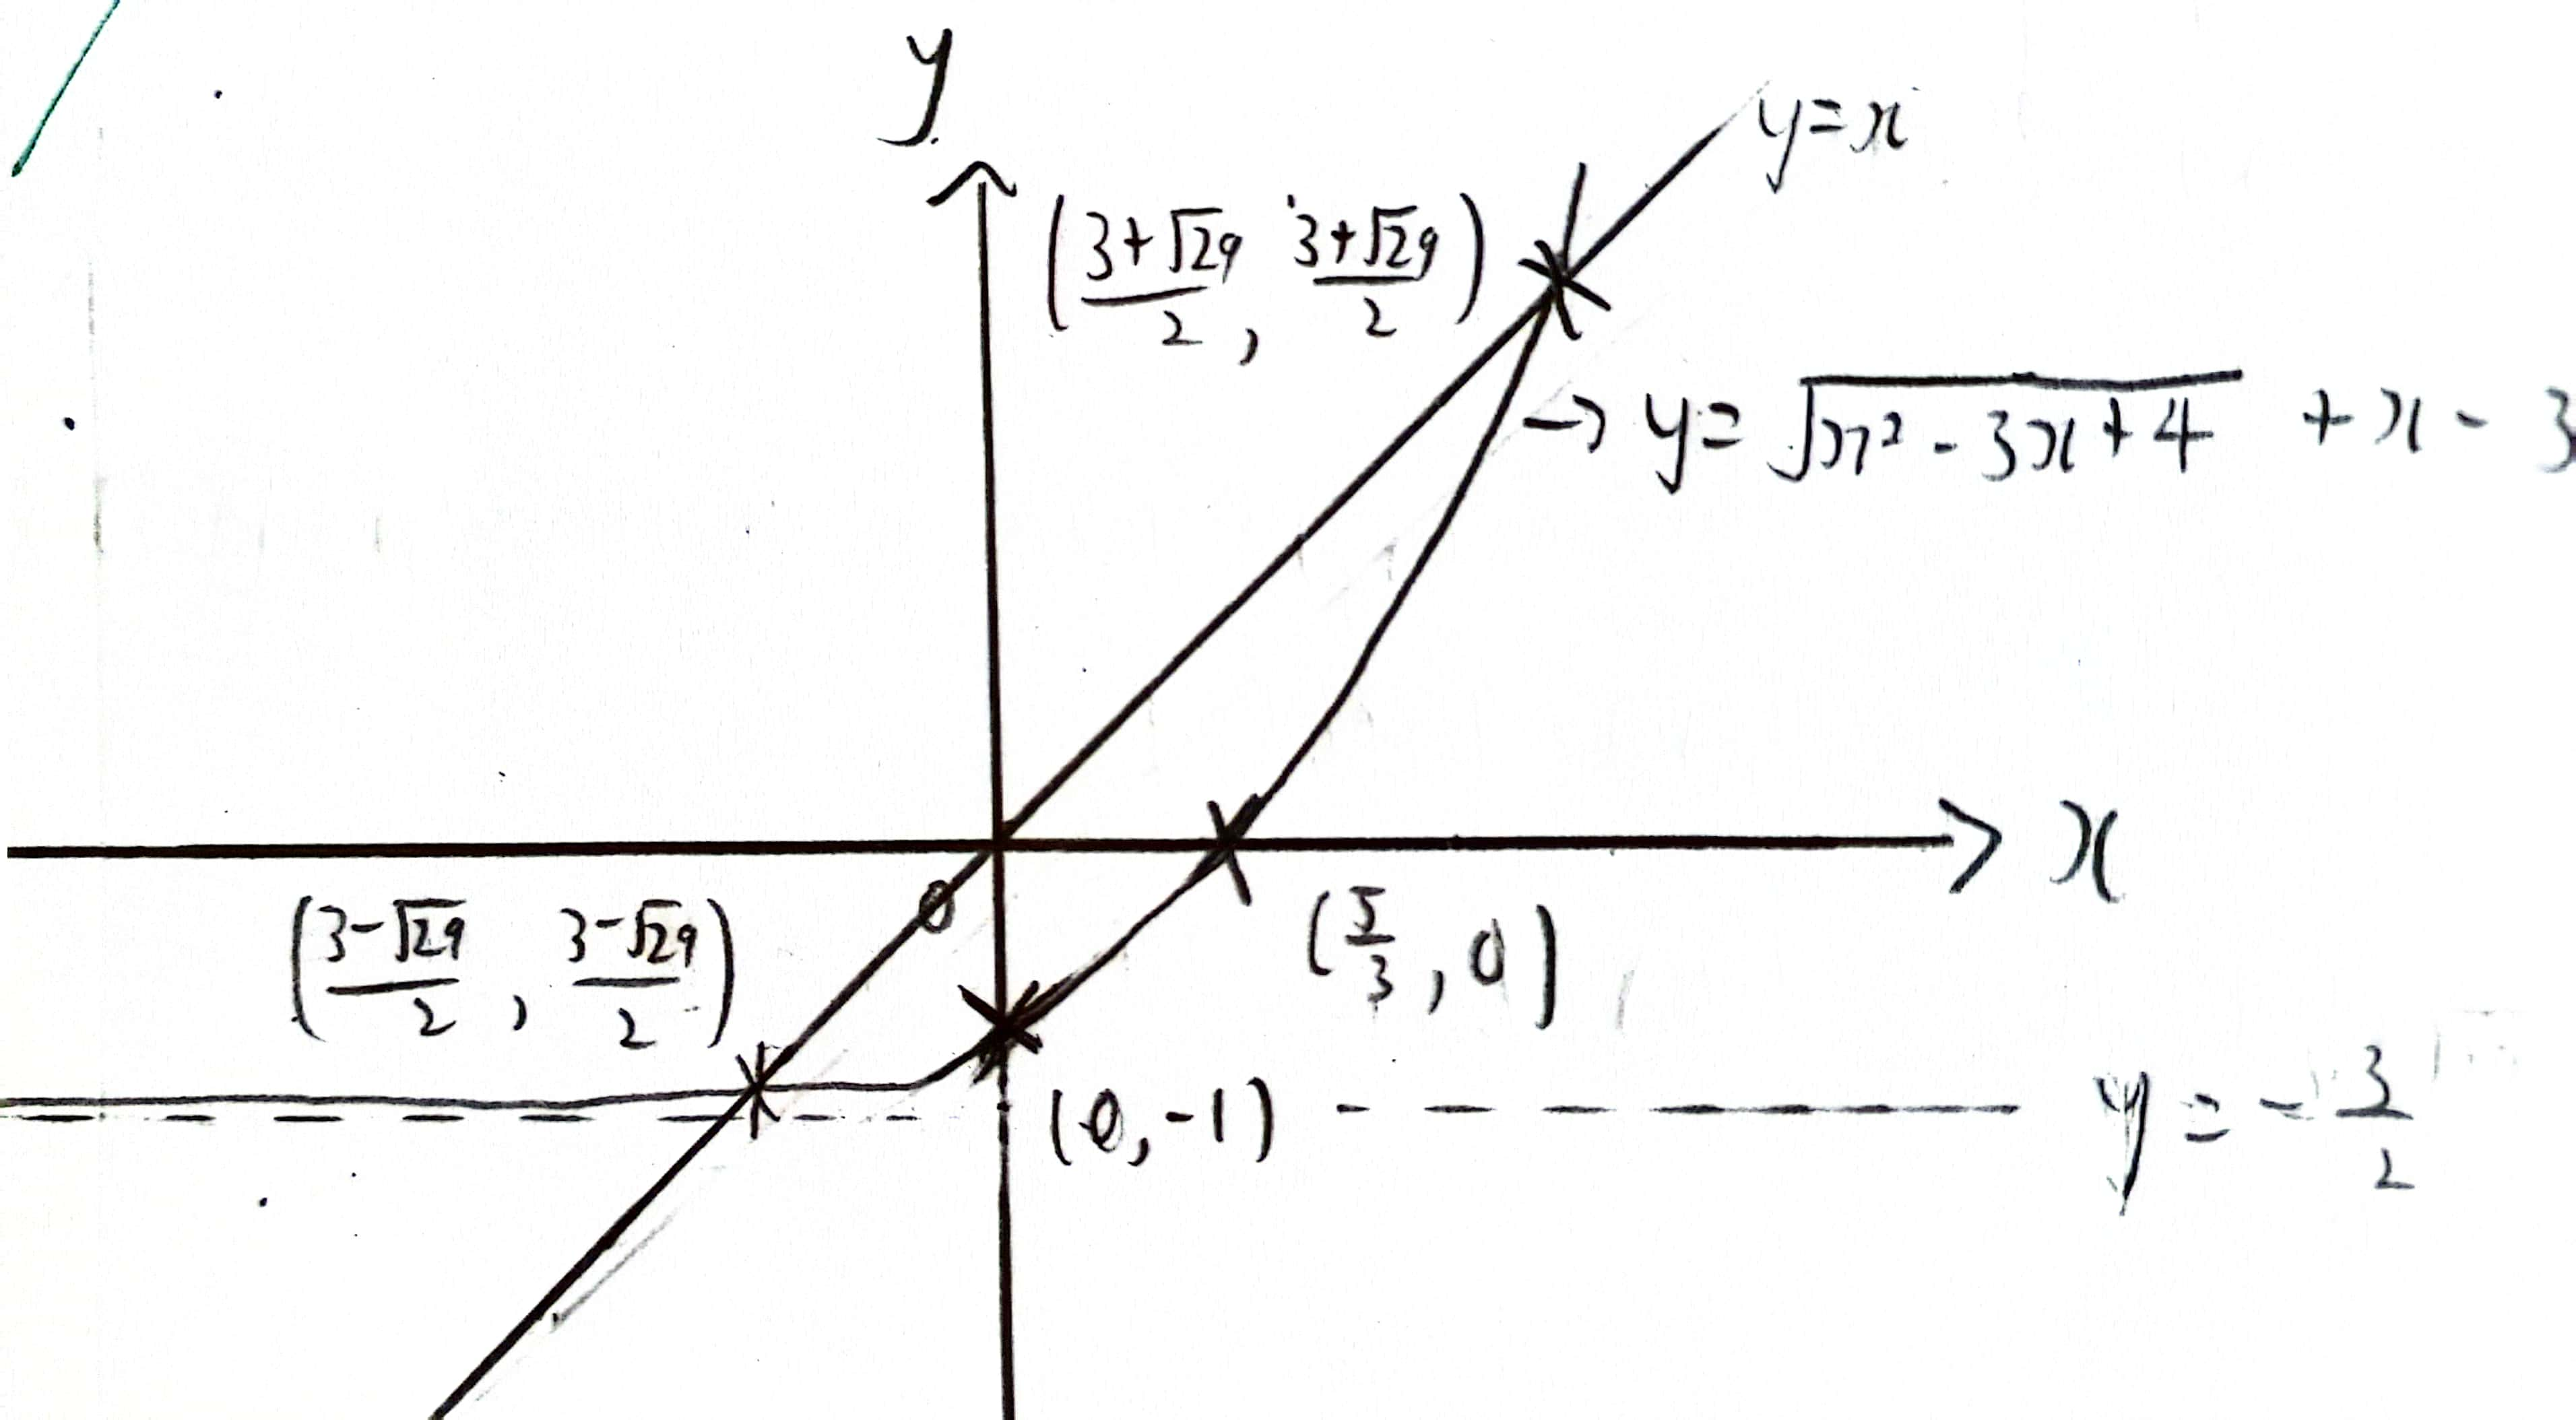
\includegraphics[scale=0.05]{SpecialRR.jpg}
    \caption{\ref{Me} The RR \(x_{n+1}=\sqrt{x_n^2-3x_n+4}+x_n-3\).}
    \label{fig:RR-identiy-function-comparison}
  \end{figure}
  \begin{center}
  \end{center}
  Let \(f(x)=\sqrt{x^2-3x+4}+x-3\).
  \begin{enumerate}
    \item Suppose \(x_1 \leq \frac{3+\sqrt{29}}{2}\). For \(x_1<\frac{3-\sqrt{29}}{2}\), we see that \(f(x)>x\). So \(x_n\) increases till \(\frac{3-\sqrt{29}}{2}\). In contrast, for \(\frac{3-\sqrt{29}}{2}<x_1<\frac{3+\sqrt{29}}{2}\), we have \(f(x)<x\). Thus \(x_n\) decreases till \(\frac{3-\sqrt{29}}{2}\). Notice the graphs intersects at \(x=\frac{3-\sqrt{29}}{2}\). This suggests that \(L=\frac{3-\sqrt{29}}{2}\).
    \item Similarly, if \(x_1=\frac{3+\sqrt{29}}{2}\), then \(x_n=\frac{3+\sqrt{29}}{2}\) is a constant function; \(L=\frac{3+\sqrt{29}}{2}\).
    \item Presume that \(x_n>\frac{3+\sqrt{29}}{2}\). Then, \(f(x)>x\) tells us \(x_n\) is an increasing sequence that is unbounded. In other words, \(L\) does not exist.
  \end{enumerate}
\end{example}
\begin{note}
  When we are asked to comment on the proposed model, it is usually about how suitable it is in modelling the actual situation.
\end{note}
\begin{example}{}{}
  Investigate what the model, with these values of \(a\) and \(b\), predict about the population when \(M_0=9679\) and \(M_0=9681\), respectively. 
  \begin{enumerate}
    \item[\textcolor{green!70!black}{\checkmark}] The model predicts that the population oscillates between  approximately 2420 and 9680 for the first few values of \(n\), but eventually becomes negative at \(n=9\) and \(n=10\). Hence the proposed model is valid only for the first few years and not in the long run. 
    \item[\textcolor{red}{\(\times\)}] The proposed model is very sensitive to small changes in the initial population of the mammal. 
  \end{enumerate}
\end{example}
\chapter{Recurrence Relations}
\begin{stbox}{General Information}{}
  \begin{enumerate}
    \item Solving RRs in general:
    \begin{enumerate}
      \item Continually expand \(u_n\) in terms of \(u_{n-1}\), then in terms of \(u_{n-2}\), and so on, till an explicit formula is obtained.
      \item Alternatively, start from \(a_1\) and iteratively find \(a_2\), \(a_3\), \ldots, \(a_n\).
    \end{enumerate}
    \item Solving \(u_{n+1}=au_{n}+b\):
    \begin{enumerate}
      \item Iteration --- Apply 4(a) and use the geometric sum formula.
      \item
      \begin{enumerate}
        \item Rewrite the RR as as \(u_n-k=a(u_{n-1}-k)\), where \(k=\frac{b}{1-a}\). Let \(v_n=u_n-k\).
        \item Then, show that \(a=\frac{v_n}{v_{n-1}}\) is a constant, so that \(\{v_n\}\) is a geometric progression with first term \(v_1-k\) and common ratio \(a\). 
        \item Now, \(v_n=(u_1-k)a^{n-1}\) and \(u_n=v_n+k=(u_1-k)a^{n-1}+k\).
      \end{enumerate}
      \item \(\bigstar\) Let \(u_n=Aa^n+\frac{b}{1-a}\) and solve for the constant \(A\) using the initial conditions provided.
    \end{enumerate}
    \item Solving \(u_{n+2}=au_{n+1}+bu_n\):
    \begin{enumerate}[label=\roman*.]
      \item The characteristic equation is \(\lambda^2-a\lambda-b=0\), which has roots \(\lambda_1\) and \(\lambda_2\).
      \item The general solution is
      \[u_n=\begin{cases}
        (An+B)\lambda^n &\text{if \(\lambda=\lambda_1=\lambda_2\)},\\
        A\lambda_1^n+B\lambda_2^n &\text{if \(\lambda_1\neq\lambda_2\)},\\
        r^n[A\cos(n\theta)+B\sin(n\theta)] &\text{if \(\lambda_1=re^{i\theta}\) and \(\lambda_2=re^{-i\theta}\) are not real},
      \end{cases}\]
      where \(A\) and \(B\) are real constants. \emph{Note.} Even if \(\lambda_1\) and \(\lambda_2\) are complex, \(u_n=A\lambda_1^n+B\lambda_2^n\) is valid.
      \item Solve for the constants \(A\) and \(B\) using the initial conditions provided.
    \end{enumerate}
  \end{enumerate}
\end{stbox}
\begin{note}\hypertarget{vieta}{}
  We should remember Vieta's Formula. Consider a complex polynomial \(a_2 z^2+a_1 z+a_0\) with roots \(r_1\) and \(r_2\). Then, the sum \(r_1+r_2=-a_1/a_2\) and the product \(r_1r_2=a_0/a_2\).
\end{note}
\begin{note}
  Let \(x_{n+1}=f(x_n)\) and \(L\coloneq \lim{x_n}\). To find the possible values of \(L\), we can compare the graph of \(y=f(x)\) against the identity function \(y=x\). This is done by seeing if \(f(x)<x\), \(f(x)=x\), or \(f(x)>x\).
\end{note}
\begin{example}{}{}
  \begin{figure}[H]
    \centering
    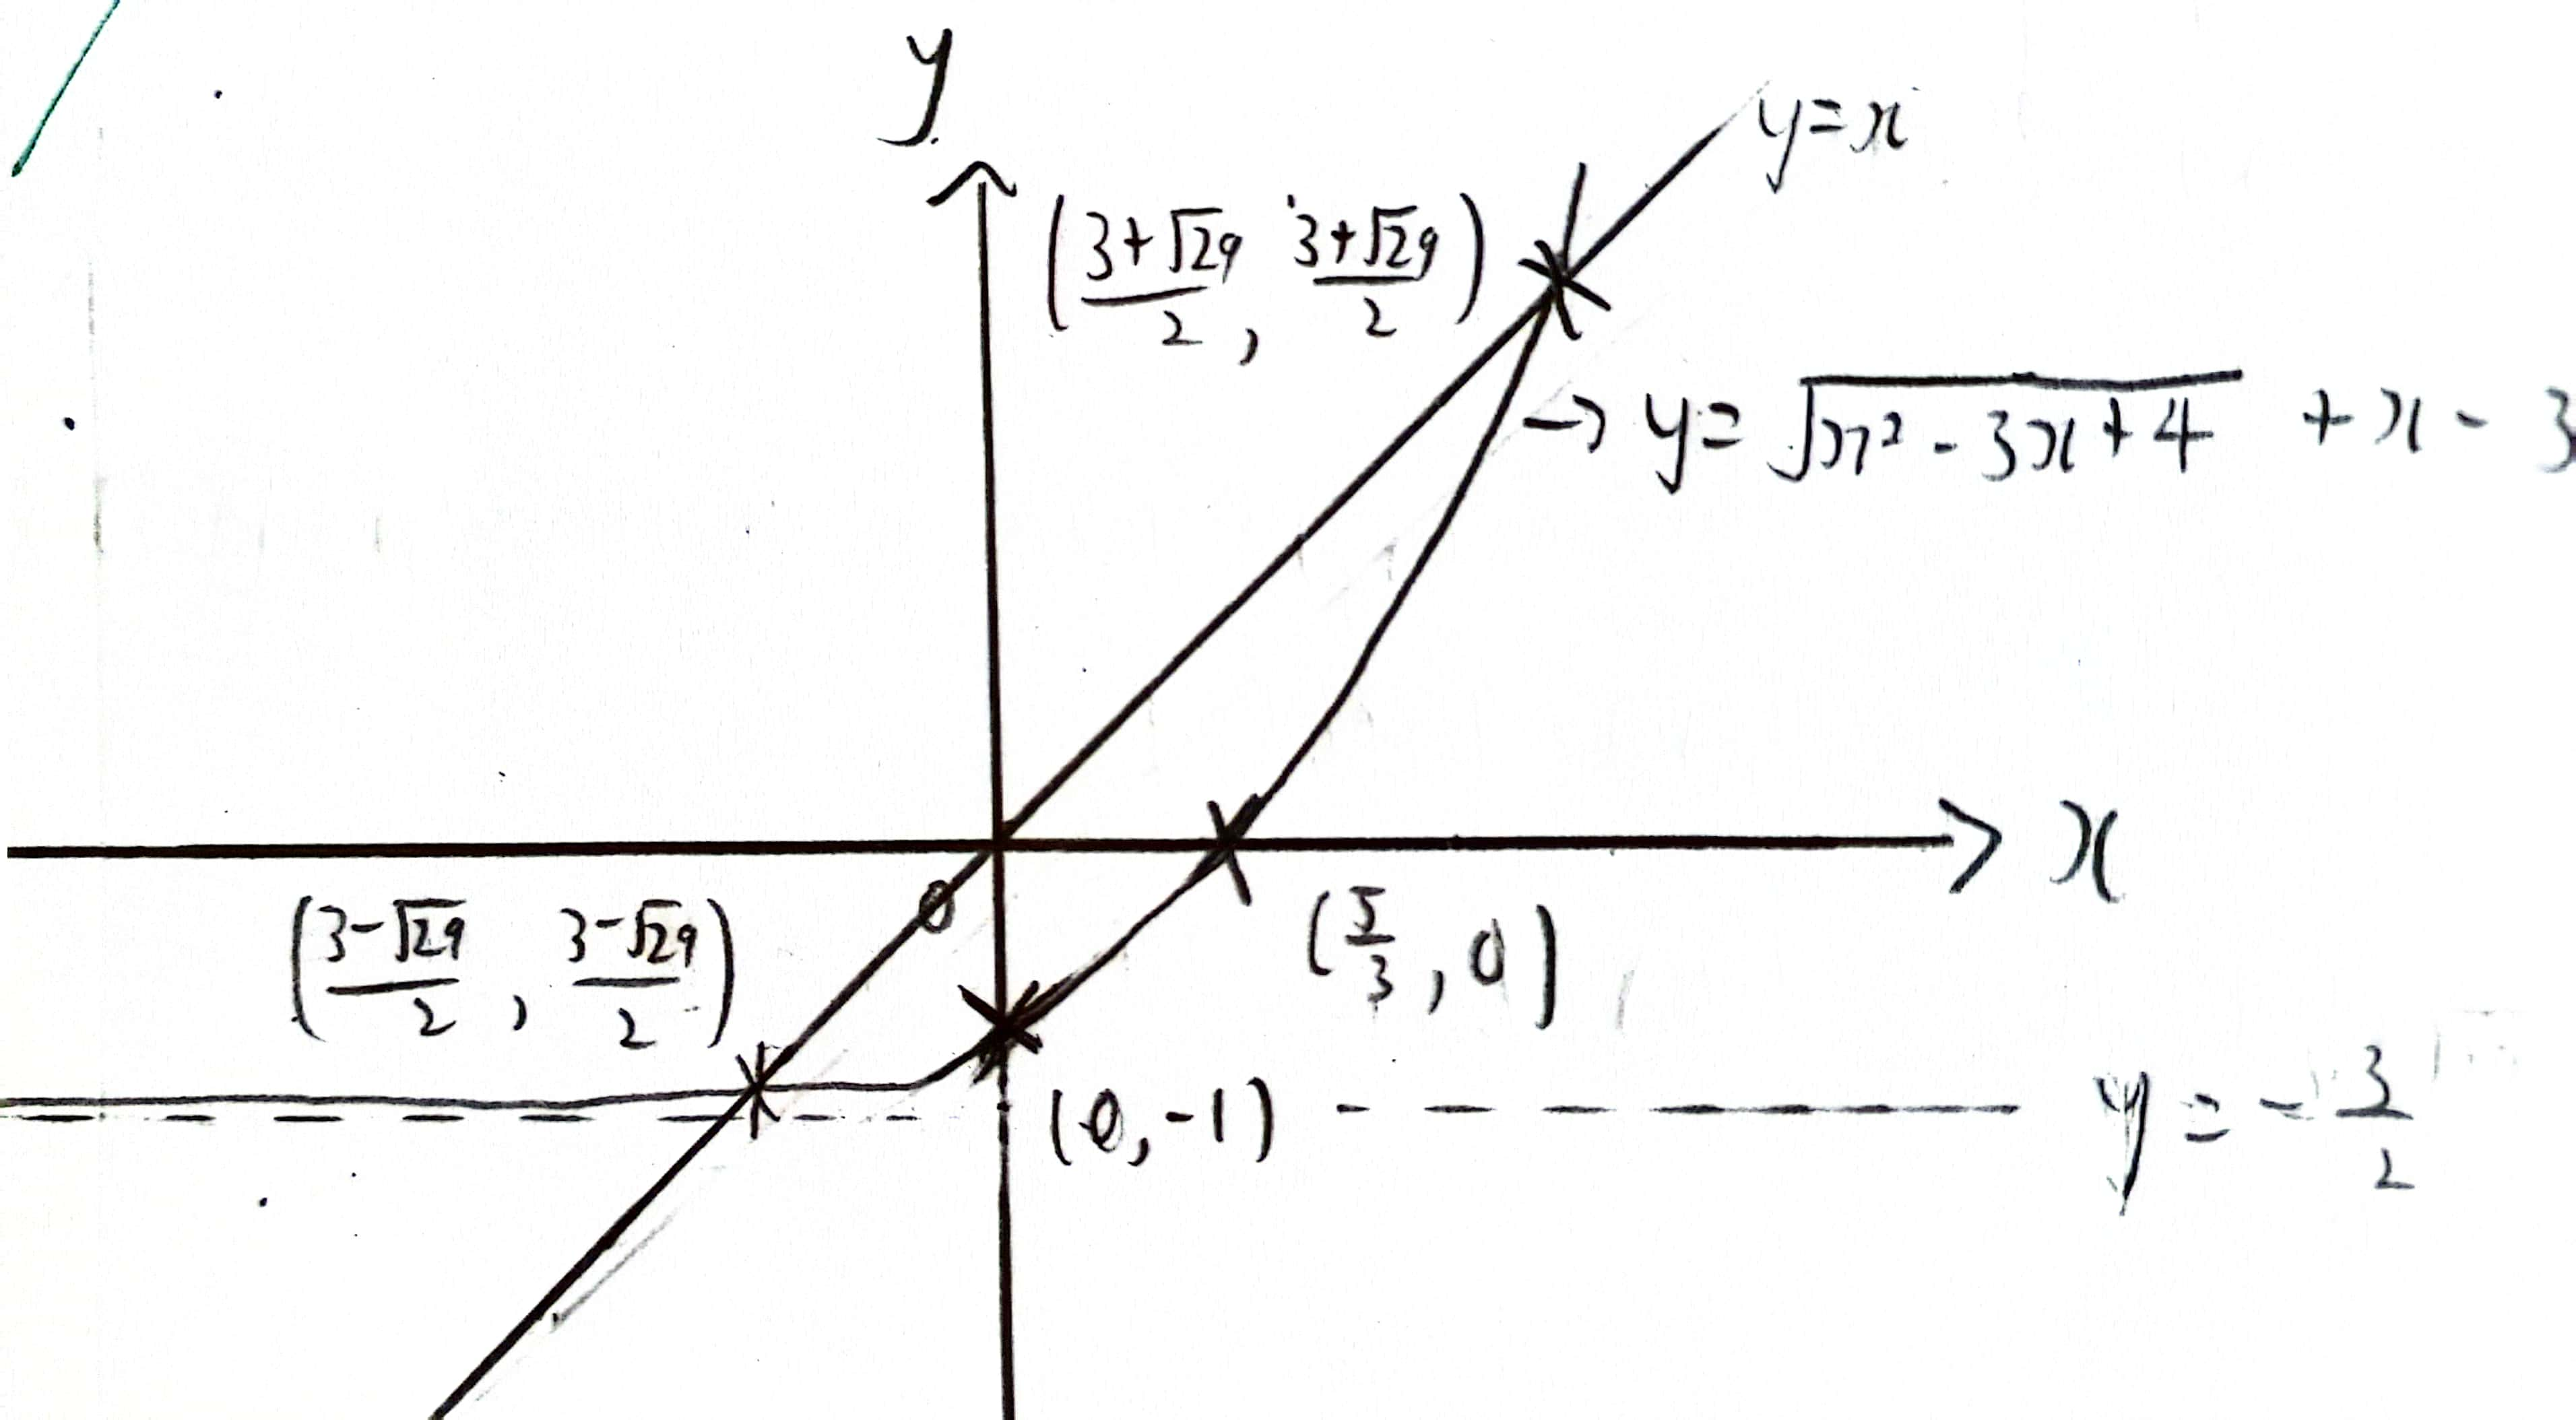
\includegraphics[scale=0.05]{SpecialRR.jpg}
    \caption{\ref{Me} The RR \(x_{n+1}=\sqrt{x_n^2-3x_n+4}+x_n-3\).}
    \label{fig:RR-identiy-function-comparison}
  \end{figure}
  \begin{center}
  \end{center}
  Let \(f(x)=\sqrt{x^2-3x+4}+x-3\).
  \begin{enumerate}
    \item Suppose \(x_1 \leq \frac{3+\sqrt{29}}{2}\). For \(x_1<\frac{3-\sqrt{29}}{2}\), we see that \(f(x)>x\). So \(x_n\) increases till \(\frac{3-\sqrt{29}}{2}\). In contrast, for \(\frac{3-\sqrt{29}}{2}<x_1<\frac{3+\sqrt{29}}{2}\), we have \(f(x)<x\). Thus \(x_n\) decreases till \(\frac{3-\sqrt{29}}{2}\). Notice the graphs intersects at \(x=\frac{3-\sqrt{29}}{2}\). This suggests that \(L=\frac{3-\sqrt{29}}{2}\).
    \item Similarly, if \(x_1=\frac{3+\sqrt{29}}{2}\), then \(x_n=\frac{3+\sqrt{29}}{2}\) is a constant function; \(L=\frac{3+\sqrt{29}}{2}\).
    \item Presume that \(x_n>\frac{3+\sqrt{29}}{2}\). Then, \(f(x)>x\) tells us \(x_n\) is an increasing sequence that is unbounded. In other words, \(L\) does not exist.
  \end{enumerate}
\end{example}
\begin{note}
  When we are asked to comment on the proposed model, it is usually about how suitable it is in modelling the actual situation.
\end{note}
\begin{example}{}{}
  Investigate what the model, with these values of \(a\) and \(b\), predict about the population when \(M_0=9679\) and \(M_0=9681\), respectively. 
  \begin{enumerate}
    \item[\textcolor{green!70!black}{\checkmark}] The model predicts that the population oscillates between  approximately 2420 and 9680 for the first few values of \(n\), but eventually becomes negative at \(n=9\) and \(n=10\). Hence the proposed model is valid only for the first few years and not in the long run. 
    \item[\textcolor{red}{\(\times\)}] The proposed model is very sensitive to small changes in the initial population of the mammal. 
  \end{enumerate}
\end{example}
\chapter{Differentiation}
\begin{definition*}{}{}
  \begin{enumerate}
    \item A function \(f\) is called (strictly) increasing on an interval \(I\) iff \(f'(x)>0\) for all \(x \in I\).
    \item A function \(f\) is called monotonically increasing on an interval \(I\) iff \(f'(x) \geq 0\) for any \(x \in I\).
  \end{enumerate}
\end{definition*}
\begin{stbox}{General Information}
  \begin{enumerate}
    \item How to sketch the graph of the integral or derivative of a function \(f\).
    \item Relationship btw. a function \(f\) and its derivative, \(f'\):\\
    \begin{center}
      \begin{tabular}{|c|c|}
        \hline
        \(y=f(x)\) & \(y=f'(x)\)\\
        \hline
        Vertical asymptote at \(x=a\) & Vertical asymptote at \(x=a\).\\
        \hline
        Horizontal asymptote at \(y=a\) & Horizontal asymptote \(y=0\).\\
        \hline
      \end{tabular}
    \end{center}
    \item Recap:\\
    \begin{center}
      \begin{tabular}{|Sc|Sc|}
        \hline
        \(f(x)\) & \(f'(x)\)\\
        \hline
        \(\sin^{-1}\left(\dfrac{x}{a}\right)\) & \(\dfrac{1}{\sqrt{a^2-x^2}}\), \(\lvert x \rvert<a\)\\
        \hline
        \(\cos^{-1}\left(\dfrac{x}{a}\right)\) & \(-\dfrac{1}{\sqrt{a^2-x^2}}\), \(\lvert x \rvert<a\)\\
        \hline
        \(\tan^{-1}\left(\dfrac{x}{a}\right)\) & \(\dfrac{a}{a+x^2}\), \(x \in \mathbb{R}\)\\
        \hline
        \(\log_a(f(x))\) &  \(\dfrac{1}{x \ln(a)}\)\\
        \hline
        \(a^x\) & \(a^x \ln(a)\)\\
        \hline
      \end{tabular}
    \end{center}
    \item Implicit differentiation: \(\dfrac{dz}{dx}=\dfrac{dz}{dy}\cdot \dfrac{dy}{dx}\).
  \end{enumerate}
\end{stbox}
\begin{note}
  Be careful when differentiating implicitly/using the chain rule. Namely, note the power \hly{two} in the following:
  \[\left( f(y)\frac{dy}{dx} \right)'=f'(y)\left( \frac{dy}{dx} \right)^{\highlight[yellow]{2}}+f(y)\frac{d^2y}{dx^2}.\]
  More generally, remember to increase the exponent of \(dy/dx\) by one with each differentiation.
\end{note}
\begin{stbox}{}
  \begin{enumerate}
    \item Small angle approximation: 
    \begin{enumerate}
      \item \(\sin(x) \approx x\),
      \item \(\cos(x) \approx 1-\dfrac{x^2}{2}\),
      \item \(\tan(x) \approx x\).
    \end{enumerate}
    \item Maclaurin Series: 
    \[f(x)=\sum_{n=0}^{\infty}\dfrac{f^{(n)}(0)}{n!}x.\]
    \item When possible, use the series --- of \(e^{x}\), \(\sin(x)\), \(\cos(x)\), et cetera --- provided in MF26 to find the required series expansion, instead of manually differentiating and applying the Maclaurin series. (Unless otherwise stated, of course.)  
  \end{enumerate}
  \begin{example*}{}{}
    Find the series expansion of \(e^{x+bx^2}\). Then, simply write
    \[e^{x+bx^2}\approx 1+(x+bx^2)+\frac{(x+bx^2)^2}{2}\approx 1+x+\left( b+\frac{1}{2} \right)x^2.\]
  \end{example*}
\end{stbox}
\chapter{Integration Techniques}
\section{Basic Integration (IBS, IBP, etc)}
\begin{stbox}{General Information}
  \begin{enumerate}
    \item Factor Formulae (remember these):
    \begin{enumerate}
      \item \(\sin(mx)\cos(nx)=\frac{1}{2}[\sin((m+n)x)+\sin((m-n)x)]\),
      \item \(\cos(mx)\cos(nx)=\frac{1}{2}[\cos((m+n)x)+\cos((m-n)x)]\),
      \item \(\sin(mx)\sin(nx)=-\frac{1}{2}[\cos((m+n)x)-\cos((m-n)x)]\).
    \end{enumerate}
    \item Common classes of integrals:
    \begin{enumerate}
      \item Apply partial fractions:
      \[\int\frac{f(x)}{g(x)}\,dx.\]
      \item Split \(px+q\), then complete the square:
      \[\int \frac{px+q}{\sqrt{ax^2+bx+c}}\,dx \quad\text{or}\quad \int \frac{px+q}{ax^2+bx+c}\,dx\] 
    \end{enumerate}
    \item Partial fractions. First ensure the numerator has a smaller degree than that of the denominator, otherwise do long division first. Then,
    \begin{flalign*}
      \text{(i)}\quad &\frac{P(x)}{(ax+b)(cx+d)}=\frac{A}{ax+b}+\frac{B}{cx+d}\\
      \text{(ii)}\quad &\frac{P(x)}{(ax+b)^2}=\frac{A}{ax+b}+\frac{B}{(ax+b)^2}\\
      \text{(iii)}\quad &\frac{P(x)}{(ax+b)(cx^2+dx+e)}=\frac{A}{ax+b}+\frac{Bx+C}{cx^2+de+e}
    \end{flalign*}
    where \(cx^2+de+e\) is irreducible, i.e. has non-real roots.
    \item Integration by Substitution: 
    \[\int f(x) \, dx=\int f(x)\frac{dx}{du}\,du.\]
    \item Use Pythagoras' Theorem / draw a right-angled triangle to help with trig conversions, e.g.:
    \[\tan(\theta) \qquad\text{to}\qquad \frac{x+1}{\sqrt{2-(x+1)^2}}.\]
    \item Integration by Parts:

    \begin{minipage}{0.5\textwidth-12.5pt}
      \begin{alignat*}{3}
        &\text{Let }& u&=\rule{0.5cm}{0.01mm} &\qquad  v&=\rule{0.5cm}{0.01mm}\\
        &&\dfrac{du}{dx} &=\rule{0.5cm}{0.01mm} & \dfrac{dv}{dx}&=\rule{0.5cm}{0.01mm}
       \end{alignat*} 
    \end{minipage}%
    \begin{minipage}{0.5\textwidth-12.5pt}
      \[\int u\left(\frac{dv}{dx}\right)\,dx=uv-\int v \left(\frac{du}{dx}\right)\,dx.\]
    \end{minipage}
  \end{enumerate}
\end{stbox}
\section{Areas \& Volumes}
\begin{figure}[H]
  \centering
  \begin{subfigure}{0.9\textwidth}
    \centering
    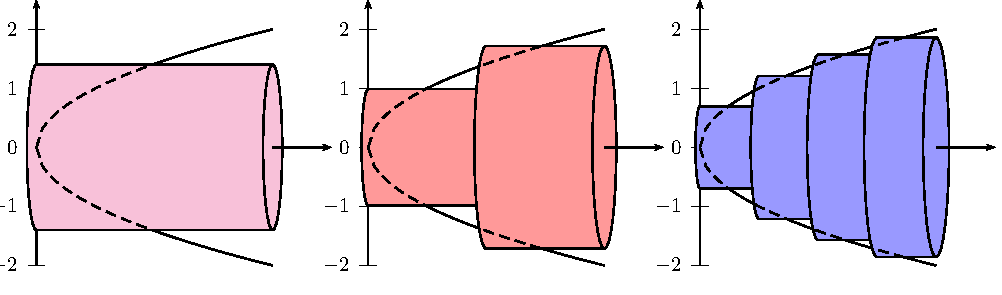
\includegraphics[width=\textwidth,page=1]{../Diagrams/disc-method/diagram2.pdf}

    \includegraphics[width=\textwidth,page=2]{../Diagrams/disc-method/diagram2.pdf}
    \caption{\(y=\sqrt{x}\)}
    \label{fig:disc-quadratic}
\end{subfigure}%

\begin{subfigure}{0.9\textwidth}
    \centering
    \includegraphics[width=\textwidth,page=3]{../Diagrams/disc-method/diagram2.pdf}

    \includegraphics[width=\textwidth,page=4]{../Diagrams/disc-method/diagram2.pdf}
    \caption{\(y=2e^{-x/2}\)}
    \label{fig:disc-func}
\end{subfigure}
  \caption{\ref{source:disc} The disc method.}
  \label{fig:disc}
\end{figure}
\begin{figure}[H]
  \centering
  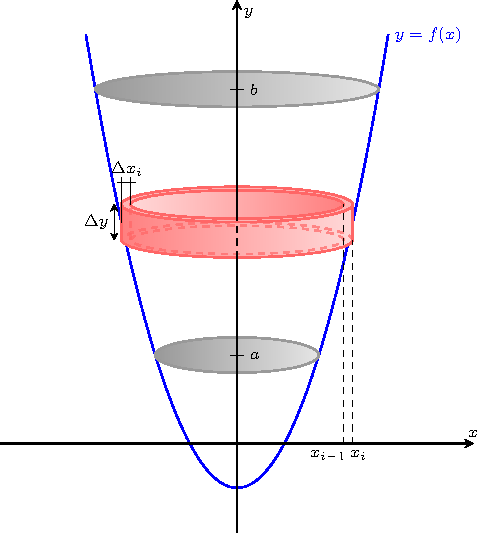
\includegraphics{../Diagrams/shell-method/diagram1.pdf}
  \caption{\ref{source:shell} The shell method.}
  \label{fig:shell}
\end{figure}
\begin{stbox}{General Information}
  \begin{enumerate}
    \item Volume of revolution when rotated about \(x\)-axis: 
  \begin{enumerate}
    \item The disc method (Figure \ref{fig:disc}):
    \[\int_{x_1}^{x_2}\pi y^2\,dx=\int_{x=x_1}^{x=x_2}\pi y^2\, \frac{dx}{dt}\,dt.\]
    \item The shell method (Figure \ref{fig:shell}):
    \[\int_{y_1}^{y_2}2\pi yx \,dy.\]
  \end{enumerate}
  \item Arc length:
  \begin{equation*}
    \resizebox{0.9\hsize}{!}{\(\displaystyle\int_{x_1}^{x_2}\sqrt{\left(\frac{dy}{dx}\right)^2+1}\,dx=\int_{y_1}^{y_2} \sqrt{\left(\frac{dx}{dy}\right)^2+1}\,dy=\int_{t_1}^{t_2}\sqrt{\left(\frac{dy}{dt}\right)^2+\left(\frac{dx}{dt}\right)^2}\,dt=\int_{\alpha}^{\beta}\sqrt{r^2+\left(\frac{dr}{d\theta}\right)^2}\,d\theta.\)}
    \end{equation*}
  \item Surface area of revolution when rotated about \(\highlight[blue!30]{x}\)-axis: 
  \begin{equation*}
    \resizebox{0.9\hsize}{!}{\(\displaystyle\int_{x_1}^{x_2}2\pi \highlight[red!30]{y} \sqrt{\left(\frac{dy}{dx}\right)^2+1}\,dx=\int_{y_1}^{y_2}2\pi \highlight[red!30]{y} \sqrt{\left(\frac{dx}{dy}\right)^2+1}\,dy=\int_{t_1}^{t_2}2\pi \highlight[red!30]{y} \sqrt{\left(\frac{dy}{dt}\right)^2+\left(\frac{dx}{dt}\right)^2}\,dt.\)}
    \end{equation*}
  \begin{flushleft}
    \(\bigstar\) Rotating about \(\highlight[blue!30]{x}\)-axis \(\implies\) \(\highlight[red!30]{y}\) in integrand\\
    \hphantom{\(\bigstar\)} Rotating about \(\highlight[blue!30]{y}\)-axis \(\implies\) \(\highlight[red!30]{x}\) in integrand.
  \end{flushleft}
  \item Area enclosed by a polar curve:
  \[\int_{\alpha}^{\beta}\frac{1}{2}r^2\,d\theta.\]
  \end{enumerate}
\end{stbox}
\begin{example}{Geometrical interpretation of an approximate area}{}
  An parabolic arc has equation \(x=at^2\), \(y=2at\) for \(0\leq t\leq p\). When rotated through \(2\pi\) radians about the \(x\)-axis, the surface area of revolution formed is \(A=8\pi a^2/3\left[ (p^2+1)^{3/2}-1 \right]\) units\(^2\). Consider the approximation to \(A\) when \(p\) is sufficiently small, such that powers above \(p^2\) can be ignored. Interpret this approximate area geometrically.
  \[A\approx 8/3\pi a^2[1+3/2p^2-1]=4\pi a^2p^2\text{ units}^2\ (=\pi(2ap)(2ap)).\]
  Geometric interpretation: The approximate area is the surface area of a cone with radius \(2ap\) and approximate slant height \(2ap\). 
  \begin{figure}[H]
    \centering
    \begin{subfigure}{0.475\textwidth}
      \centering
      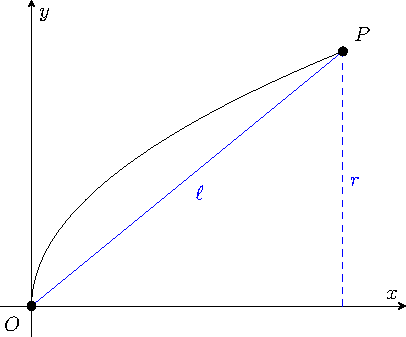
\includegraphics[width=\textwidth]{../Diagrams/approximate-surface-area/curve.pdf}
      \caption{2d illustration.}
  \end{subfigure}\hfill
  \begin{subfigure}{0.475\textwidth}
      \centering
      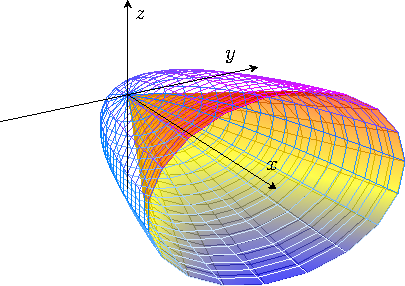
\includegraphics[width=\textwidth]{../Diagrams/approximate-surface-area/3d.pdf}
      \caption{3d illustration.}
  \end{subfigure}
    \caption{\ref{Me}}
    \label{fig:surface-area}
  \end{figure}
  \emph{Note.} The slant height \(\ell=\sqrt{(ap^2)^2+(2ap)^2}=\sqrt{a^2p^4+4a^2p^2}\approx\sqrt{a^2\cdot 0+4a^2p^2}=2ap\).
\end{example}
\section{Numerical Methods}
\subsection{Trapezium Rule}
\begin{stbox}{General Information}
    \begin{enumerate}
      \item Formula for \(n\) intervals, or (n+1)ordinates, of width \(h\coloneq (b-a)/n\): 
      \[\int_{a}^{b}y\,dx=\frac{h}{2}(y_0+2y_1+2y_2+\cdots+2y_{n-1}+y_n).\]
      \item Illustration
      \begin{figure}[H]
        \centering
        \includestandalone{../Diagrams/Trapezium}
        \caption{\ref{source:trapzium-rule} Trapezium rule.}
        \label{fig:trapzium-rule}
      \end{figure}
    \item Error: 
    \begin{enumerate}
      \item Concave upwards, i.e. (\(f'(x)\) is increasing / \(f''(x)>0\)) \(\implies\) overestimation.
      \item Concave downwards, i.e. (\(f'(x)\) is decreasing / \(f''(x)<0\)) \(\implies\) underestimation.
    \end{enumerate}
    \end{enumerate}
    \end{stbox}
    \begin{note}
      State and explain whether the trapezium rule gives an underestimate or an overestimate of the area of under the curve \(y=f(x)\) from \(x=x_0\) to \(x=x_1\).
      \begin{figure}[H]
        \centering
        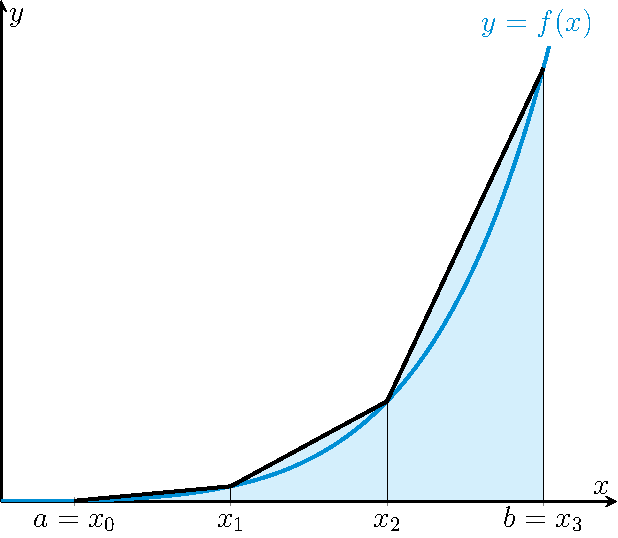
\includegraphics[width=0.4\textwidth]{../Diagrams/trapzium-estimate.pdf}
        \caption{\ref{source:trapzium-rule} The trapezium rule results in an overestimate for the area under a curve that is concave upwards.}
        \label{fig:trapezium-overestimate}
      \end{figure}
      From the diagram and the fact that \(\frac{d^2y}{dx^2}=\rule{0.5cm}{0.01mm}>0\) for all \(x\in[a,b]\), the curve is concave upwards. As such, the trapeziums contain the graph of \(y=f(x)\), for \(x\in[a,b]\). So, the trapezium rule gives a overestimate.
    \end{note}
    \subsection{Simpson's Rule}
    \begin{stbox}{General Information}
      \begin{enumerate}
        \item Formula for \(n\) intervals, or (n+1)ordinates, of width \(h\coloneq (b-a)/n\):
        \[\int_{a}^{b}y\,dx=\frac{h}{3}(y_0+4y_1+2y_2+4y_3+\cdots+2y_{n-2}+4y_{n-1}+y_n).\]
        Note that the number of intervals \(n\) should be \emph{even}, that of ordinates \emph{odd}.
        \item Illustration
        \begin{figure}[H]
          \centering
          \includestandalone{../Diagrams/Simpson}
          \caption{\ref{source:simpson's-rule} Simpson's rule.}
          \label{fig:simpson's-rule}
        \end{figure}
        \item Simpson's Rule is exact for all polynomials of degree three and below.
      \end{enumerate}
    \end{stbox}
    \begin{example}{}{}
      Explain, with the aid of a suitable diagram, why Simpson's Rule does not give a good approximation of the value of \(I=\int_{a}^{b}f(x)\,dx\) and suggest how the method can be improved to give a better approximation.

      \rule{20cm-137.0549pt-25pt}{0.05mm}

      \begin{figure}[H]
        \centering
        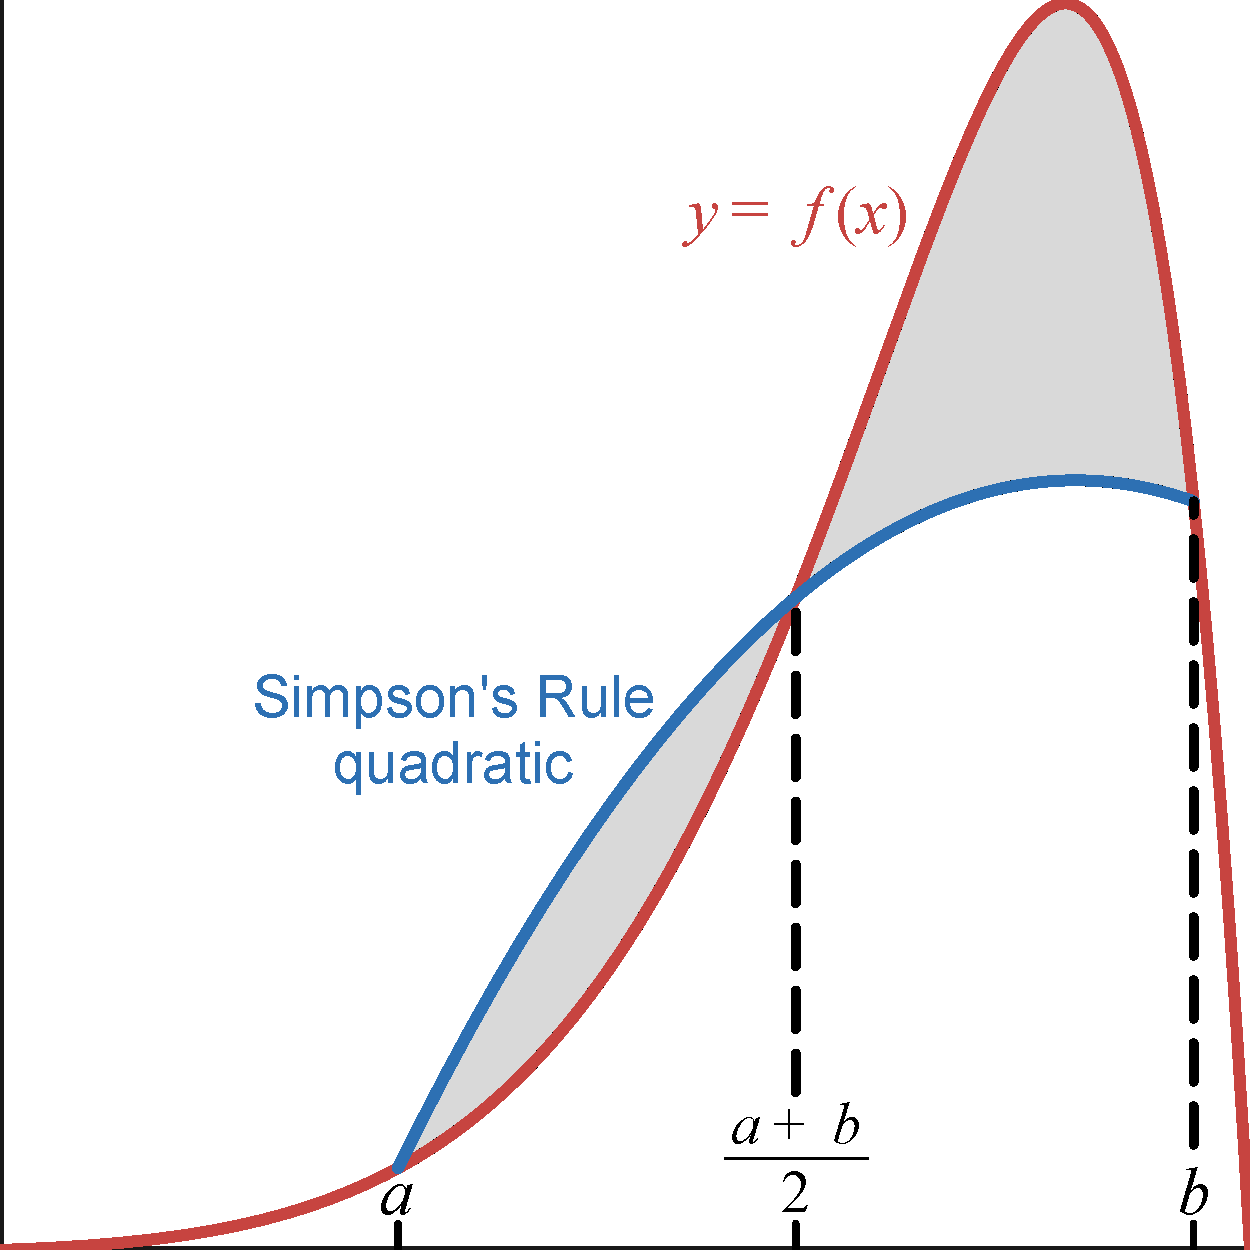
\includegraphics[width=0.425\textwidth]{../Diagrams/simpson-underestimate.pdf}
        \caption{\ref{Me} \href{https://www.desmos.com/calculator/wxxs9ypjkf}{(Desmos)}}
        \label{fig:simpson's-rule-overestimate-prelims}
      \end{figure}
      We see that there is a large discrepancy between the area under the actual curve \(y=f(x)\) and the approximated quadratic curve for the interval \(a\leq x\leq b\), which is caused by [the existence of both a turning point and a point of inflection]. Hence, Simpson's Rule using \(n\) ordinates will not provide a good approximation in this case.
    \end{example}
    \begin{note}
      Accuracy of the Trapezium rule vs Simpson's Rule:
      ``Simpson's Rule uses \emph{quadratic curves} to interpolate the points on the curve so it usually \emph{gives a better approximation} to the actual curve than the trapezium rule which uses \emph{straight lines} to interpolate the ordinates.''
    \end{note}
\section{Reduction formulas}
\begin{stbox}{General Information}{}
  Let \(I_n\coloneq\int_{a}^{b}f(x)\,dx\). To find a reduction formula for \(I_n\), we use integration by parts on \(I_n\).

  \emph{Note.} Integrating \(I_{n-1},I_{n+1},\text{etc}\) (by parts) typically does not produce nice results.  
\end{stbox}
Sometimes, some algebraic tricks are needed to reduce an integral into the desired form. Try to spot these, before attempting another round of integration by parts. 
\begin{example}{Rewriting \(x^2\) as \((4-x^2)-4\)}{}
  % \begin{alignat*}{3}
  %   &\text{Let }& u&=\dfrac{1}{(4-x^2)^n} &\qquad  v&=1\\
  %   &&\dfrac{du}{dx} &=\dfrac{2nx}{(4-x^2)^{n+1}} & \dfrac{dv}{dx}&=x
  %  \end{alignat*}
  Using
   \begin{alignat*}{2}
    u&=\dfrac{1}{(4-x^2)^n} &\qquad  v&=1\\
    \dfrac{du}{dx} &=\dfrac{2nx}{(4-x^2)^{n+1}} & \dfrac{dv}{dx}&=x
   \end{alignat*}
   we evaluate \(A_n\coloneq\int_{0}^{1/2}\frac{1}{(4-x^2)^n}\,dx\):
{\allowdisplaybreaks
     \begin{align*}
    A_n&=\frac{1}{2}{\left( \frac{4}{15} \right)^n}-2n\int_{0}^{1/2}\frac{x^2}{(4-x^2)^{n+1}}\,dx\\
    &=\frac{1}{2}{\left( \frac{4}{15} \right)^n}+2n\int_{0}^{1/2}\frac{\highlight[yellow]{(4-x^2)-4}}{(4-x^2)^{n+1}}\,dx\\
    &=\frac{1}{2}{\left( \frac{4}{15} \right)^n}+2n\int_{0}^{1/2}\frac{4-x^2}{(4-x^2)^n}-4\cdot\frac{1}{(4-x^2)^{n+1}}\,dx\\
    &=\frac{1}{2}{\left( \frac{4}{15} \right)^n}+2n(A_n-4A_{n+1}).\\
   \end{align*}}
   Therefore, \((2n-1)A_n+1/2(4/15)^n=8nA_{n+1}\).
\end{example}
\chapter{Complex Numbers}
  \section{Complex Number I}
  \begin{figure}[H]
    \centering
    \includegraphics[page=145,width=\textwidth]{../Diagrams/Argand.pdf}
    \caption{\ref{source:complex-polar} The polar representation of a complex number.}
    \label{fig:complex-polar}
  \end{figure}
  \begin{stbox}{General Information}
    \begin{enumerate}
      \item Find the square root of \(x+iy\): Let \(\sqrt{x+iy}=a+bi\). Then square both sides \& solve.
      \item Simplifying fractions: multiply by the denominator's conjugate
      \[\frac{a+bi}{c+di}=\frac{a+bi}{c+di}\cdot\frac{c-di}{c-di}=\cdots.\]
      \item Polynomials:
      \begin{enumerate}
        \item Fundamental Theorem of Algebra: If \(p(z)\coloneq \sum_{i=0}^{n}a_iz^i\) is a polynomial of degree \(n \geq 1\) with complex coefficients, then there exists complex numbers \(c_i\) for each \(1 \leq i \leq n\) such that 
        \[p(z)=a_n \prod_{i=1}^{n}(z-c_i).\]
        \item If a polynomial in real coefficients only has root \(a+bi\), then \(a-bi\) is another root.
      \end{enumerate}
    \end{enumerate}
    \end{stbox}
        \begin{example}{}{}
          Find the roots of \(iz^2+2z+3i=0\).
          \begin{align*}
            z^2-2iz+3&=0\\
            z&=\frac{2i \pm \sqrt{(2i)^2-4(1)(3)}}{2(1)}=i \pm \frac{\sqrt{-16}}{2}=i \pm 2i
          \end{align*}
          So, \(z=3i\) or \(z=-i\).
        \end{example}
        \begin{example}{N2010/2/1}{}
          One root of the equation \(x^4+4x^3+ax+b=0\), where \(a\) and \(b\) are real, is \(x=-2+i\). Find the values of \(a\) and \(b\) and the other roots.\\[3mm]
          Substitute \(-2+i\) into the equation:
          \begin{align*}
            (-2+i)^4+4(-2+i)^3+(-2+i)^2+a(-2+i)+b&=0\\
            -12+16i&=2a-b-ai\\
            a=-16, &\hphantom{=}\ \ 2a-b=-12
          \end{align*}
          Therefore, \(a=-16\), \(b=-20\).\\[3mm]
          \emph{Since all the coefficients of the polynomial are real} (\textbf{explain}), \(-2-i\) is another root. Now, \(x^4+4x^3+ax+b=(x-(-2+i))(x-(-2-i))(cx+d)\) for some \(c,d \in \mathbb{R}\).\\[3mm]
          Accordingly, substitute \(x=0\), then \(x=2\), and solve. Alternatively, notice \(x^4+4x^3+ax+b=(x^2-2(-2)x+((-2)^2+1^2))(x^2+cx+d)=(x^2+4x+5)(x^2+4x+5)\). Either ways, we have \(c=0\) and \(d=-4\). As such, the last two roots are \(x=-2 \pm i\) and \(x=\pm 2\). 
        \end{example}
      \begin{stbox}{}
        \begin{itemize}[label=\hphantom{1.}]
          \item
          \begin{enumerate}[label=(\alph*)]
            \setcounter{enumi}{2}
            \item Simultaneous equations: Solve as usual.
            \item Properties of modulus: \(\lvert z_1^xz_2^y \rvert=\lvert z_1 \rvert^x \lvert z_2 \rvert^y\), for any \(x,y \in \mathbb{R}\).
            \item Properties of arguments (same as \(\log\)): \(\arg(z) \in (-\pi,\pi]\) and \(\arg(z_1^xz_2^y)=x\arg(z_1)+y\arg(z_2)\) for any \(x,y \in \mathbb{R}\).
            \item Polar form: \(z=re^{i\theta}\).
            \item Polar/Trigonometric form: \(z=r[\cos(\theta)+i\sin(\theta)]\).
          \end{enumerate}
        \end{itemize}
  \end{stbox}
  \begin{note}
    Show that the value of \(w^n\) is either \(2^n\) or \(2^{-n}\) for integers \(n\).\\[3mm]
    Then we \textbf{must} show that \(w^n=\cdots=\begin{cases}
      2^n(1)=2^n&\text{if }n\text{ even},\\
      2^n(-1)=-2^n&\text{if }n\text{ odd}.
    \end{cases}\) 
  \end{note}
  \begin{note}
    Common tricks to know:
    \begin{enumerate}
      \item Replace all occurrences of \(w\) in a polynomial \(P(x)\) with \(-w\).
      \item Notice that a geometric series is being used. E.g. \(\frac{1}{z^2}-\frac{1}{z}+1-z+z^2=\frac{z^5+1}{z^2(z+1)}\). 
    \end{enumerate}
  \end{note}
\section{Complex Numbers II}
\begin{theorem}{De Moivre's Theorem}{}
  Let \(z\) be a complex number, \(n\) an integer, and \(\theta\) an angle. Suppose \(z=re^{i\theta}\). Then, 
  \[z^n=r^ne^{in\theta}=r^n[\cos(n\theta)+i\sin{n\theta}].\]
\end{theorem}
\begin{stbox}{General Information}
  \begin{enumerate}
    \item All \(n\)th roots of any complex number are the same distance \(r\) from the origin and have the same angular separation, \(\pi/n\).
    \item Note that \(1+e^{i\theta}=e^{i\theta/2}(e^{-i\theta/2}+e^{i\theta/2})\).
    \item For \(z=re^{i\theta}\), we have \(z^n+z^{-n}=2\cos(n\theta)\) and \(z^n-z^{-n}=2i\sin(n\theta)\).
    \item The geometric meaning of multiplying by \(i\) is a anti-clockwise rotation by \(\pi\) radians.
    \item To represent roots of unity on an argand diagram, we should annotate 
    \begin{enumerate}
      \item The points representing the roots, as dots.
      \item The (dotted) circle which these points lie on.
      \item The radius of the circle.
      \item The angular separation between the roots.
    \end{enumerate}
    \begin{figure}[H]
      \centering
      \includegraphics[width=0.4\textwidth,page=2]{../Diagrams/Complex-revision.pdf}
      \caption{\ref{Me} Roots of unity on an argand diagram.}
      \label{fig:roots-of-unity}
    \end{figure}
    \item Loci (Use a \emph{compass})
    \begin{enumerate}
      \item The locus represented by \(\lvert z-a \rvert =r\) (or \(z=a+re^{i\theta}\)) is a \emph{circle} of radius \(r\) centered at \(A(x,y)\) (where \(a\coloneq x+iy\)).
      \begin{figure}[H]
        \centering
        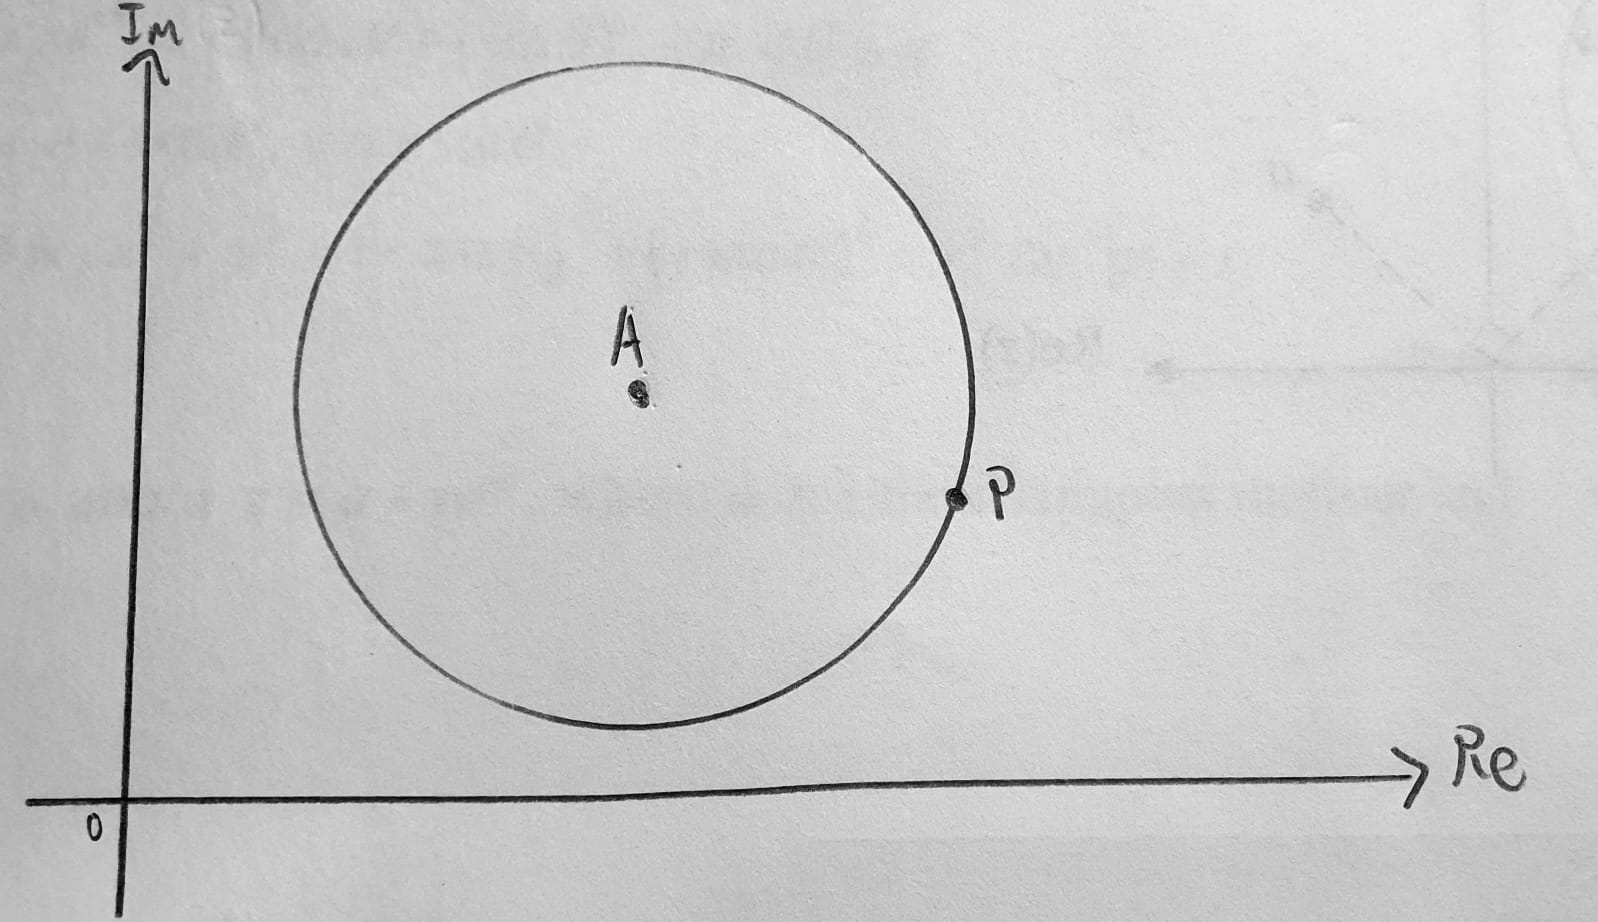
\includegraphics[scale=0.1]{../images/ComplexCircleLocus}
        \caption{\ref{Me} The locus of \(\lvert z-a \rvert =r\).}
        \label{fig:circle-locus}
      \end{figure}
      \begin{enumerate}
        \item Either label the four points to the direct North, South, East, West of the circle, or denote the radius clearly. 
        \item The line segment, representing the furthest distance from a point to a circle, always cuts through the circle's centre. So, the distance
        \[\text{OP}_{\text{max}}-\text{OP}_{\text{min}}=2\cdot\text{radius}.\]
        \item The line segments, from a point to a circle that produces the largest angle, are tangents to the circle.
        \begin{figure}[H]
          \centering
          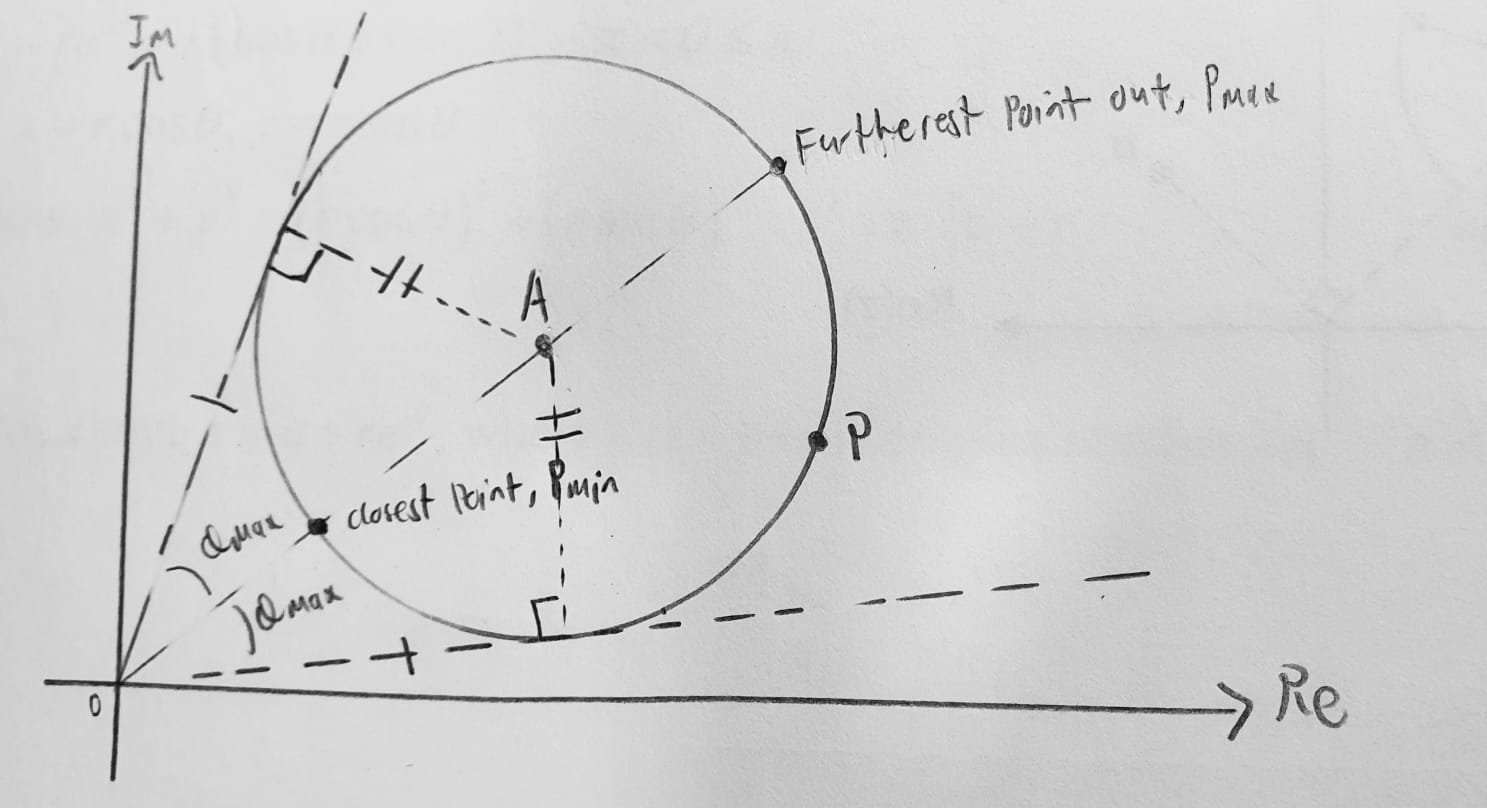
\includegraphics[scale=0.15]{ComplexLocusCircle-LargestAngleAndDistance.jpg}
          \caption{\ref{Me} Maxmium distance and angle of a point from a circle}
          \label{fig:locus-max-distance-and-angle-circle}
        \end{figure}
      \end{enumerate}
      \item The locus represented by \(\lvert z-a \rvert =\lvert z-b \rvert\) is the \emph{perpendicular bisector} of the line segment joining \(A\) and \(B\).
      \begin{figure}[H]
        \centering
        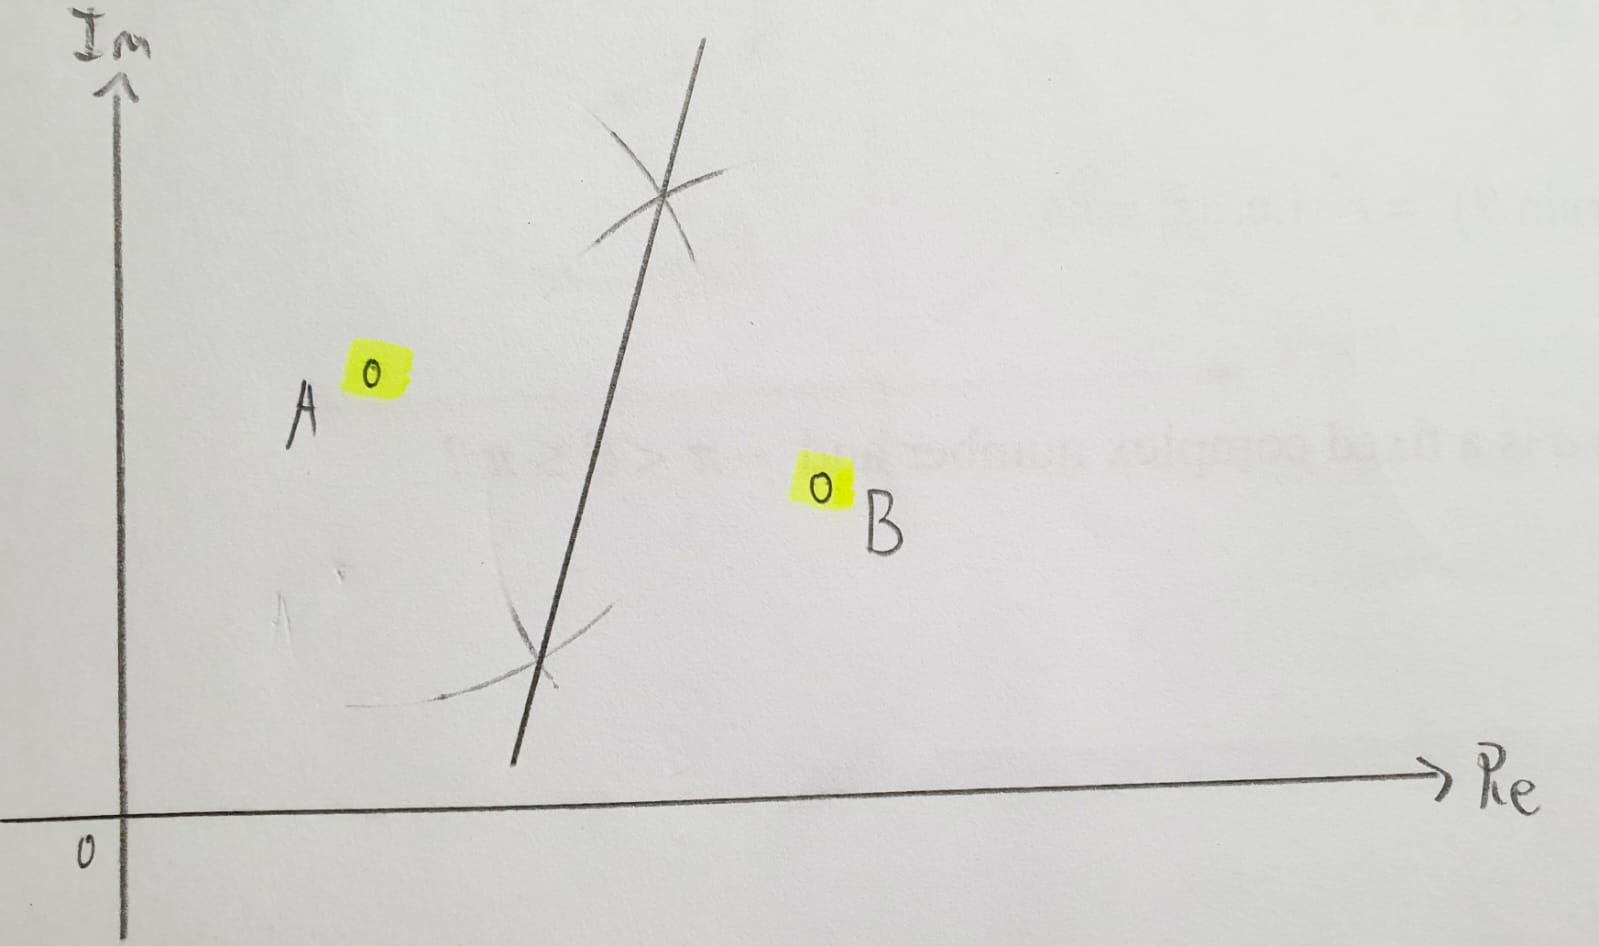
\includegraphics[scale=0.12]{../images/ComplexPerpendicularBisectorLocus}
        \caption{\ref{Me} The locus of \(\lvert z-a \rvert =\lvert z-b \rvert\), a perpendicular bisector.}
        \label{fig:perpendicular-bisector-locus}
      \end{figure}
      \item The locus represented by \(\arg(z-a)=\theta\) is the \emph{half-line} from \(A\) (excluding \(A\)) that makes an angle \(\theta\) with the \emph{positive} real axis.
      \begin{figure}[H]
        \centering
        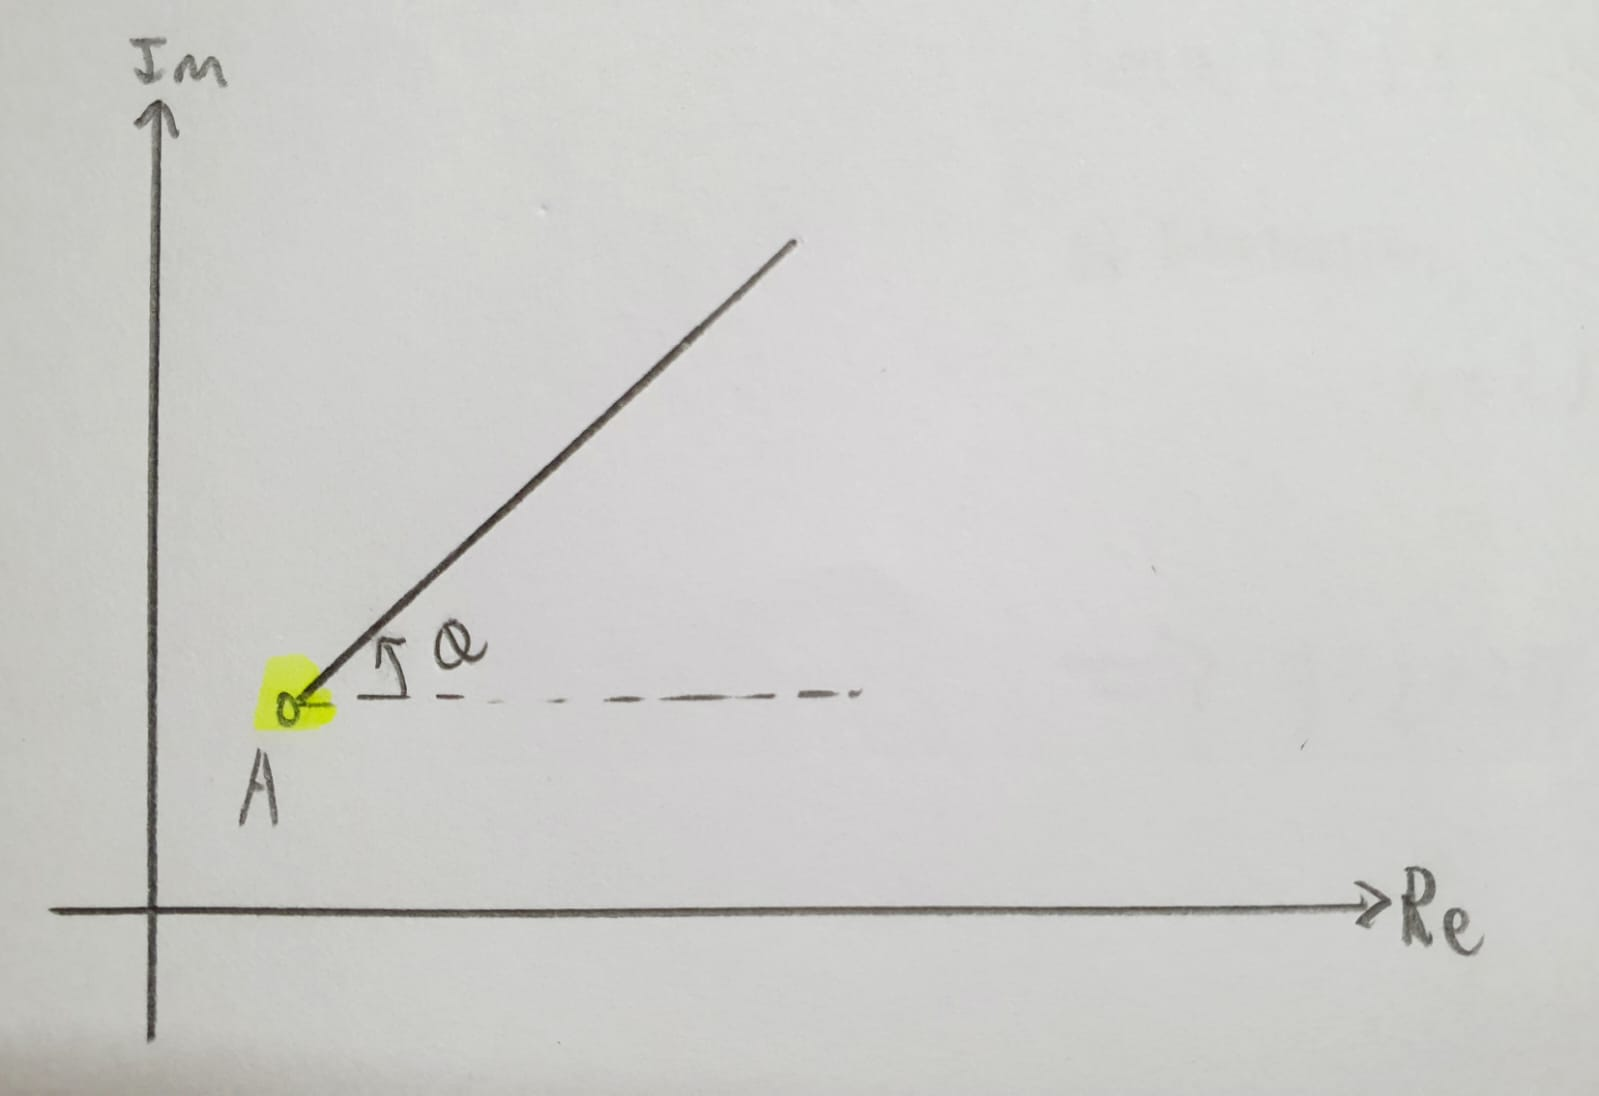
\includegraphics[scale=0.1]{../images/ComplexRotationByAngleTheta}
        \caption{\ref{Me} The locus of \(\arg(z-a)=\theta\), a half-line.}
        \label{fig:half-line-locus}
      \end{figure}
    \end{enumerate}
    \item There is no need to find the points of intersection between two loci, unless the questions states so. 
    \item Suppose we have a locus \(z\) represented by the predicate \(P(z)\). Then, for any \(a\in \mathbb{C}\), the locus of \(z+a\) is represented by \(P(z-a)\).
    \item Say we are given a locus \(z\) represented by \(\lvert z-a \rvert=r\), where \(a=\alpha+\beta i\). 
    \begin{enumerate}
      \item The greatest and least value of \(\lvert z \rvert\) are \(\lvert a \rvert \pm r\), respectively. 
      \item The greatest and least value of \(\arg(z)\) can be obtained geometrically, or by plotting 
      \[Y_1=\tan^{-1}\left(\frac{\beta\pm\sqrt{r^2-(X-\alpha)^2}}{X}\right)\]
      and finding the maximum/minimum point, respectively.
      \begin{figure}[H]
        \centering
        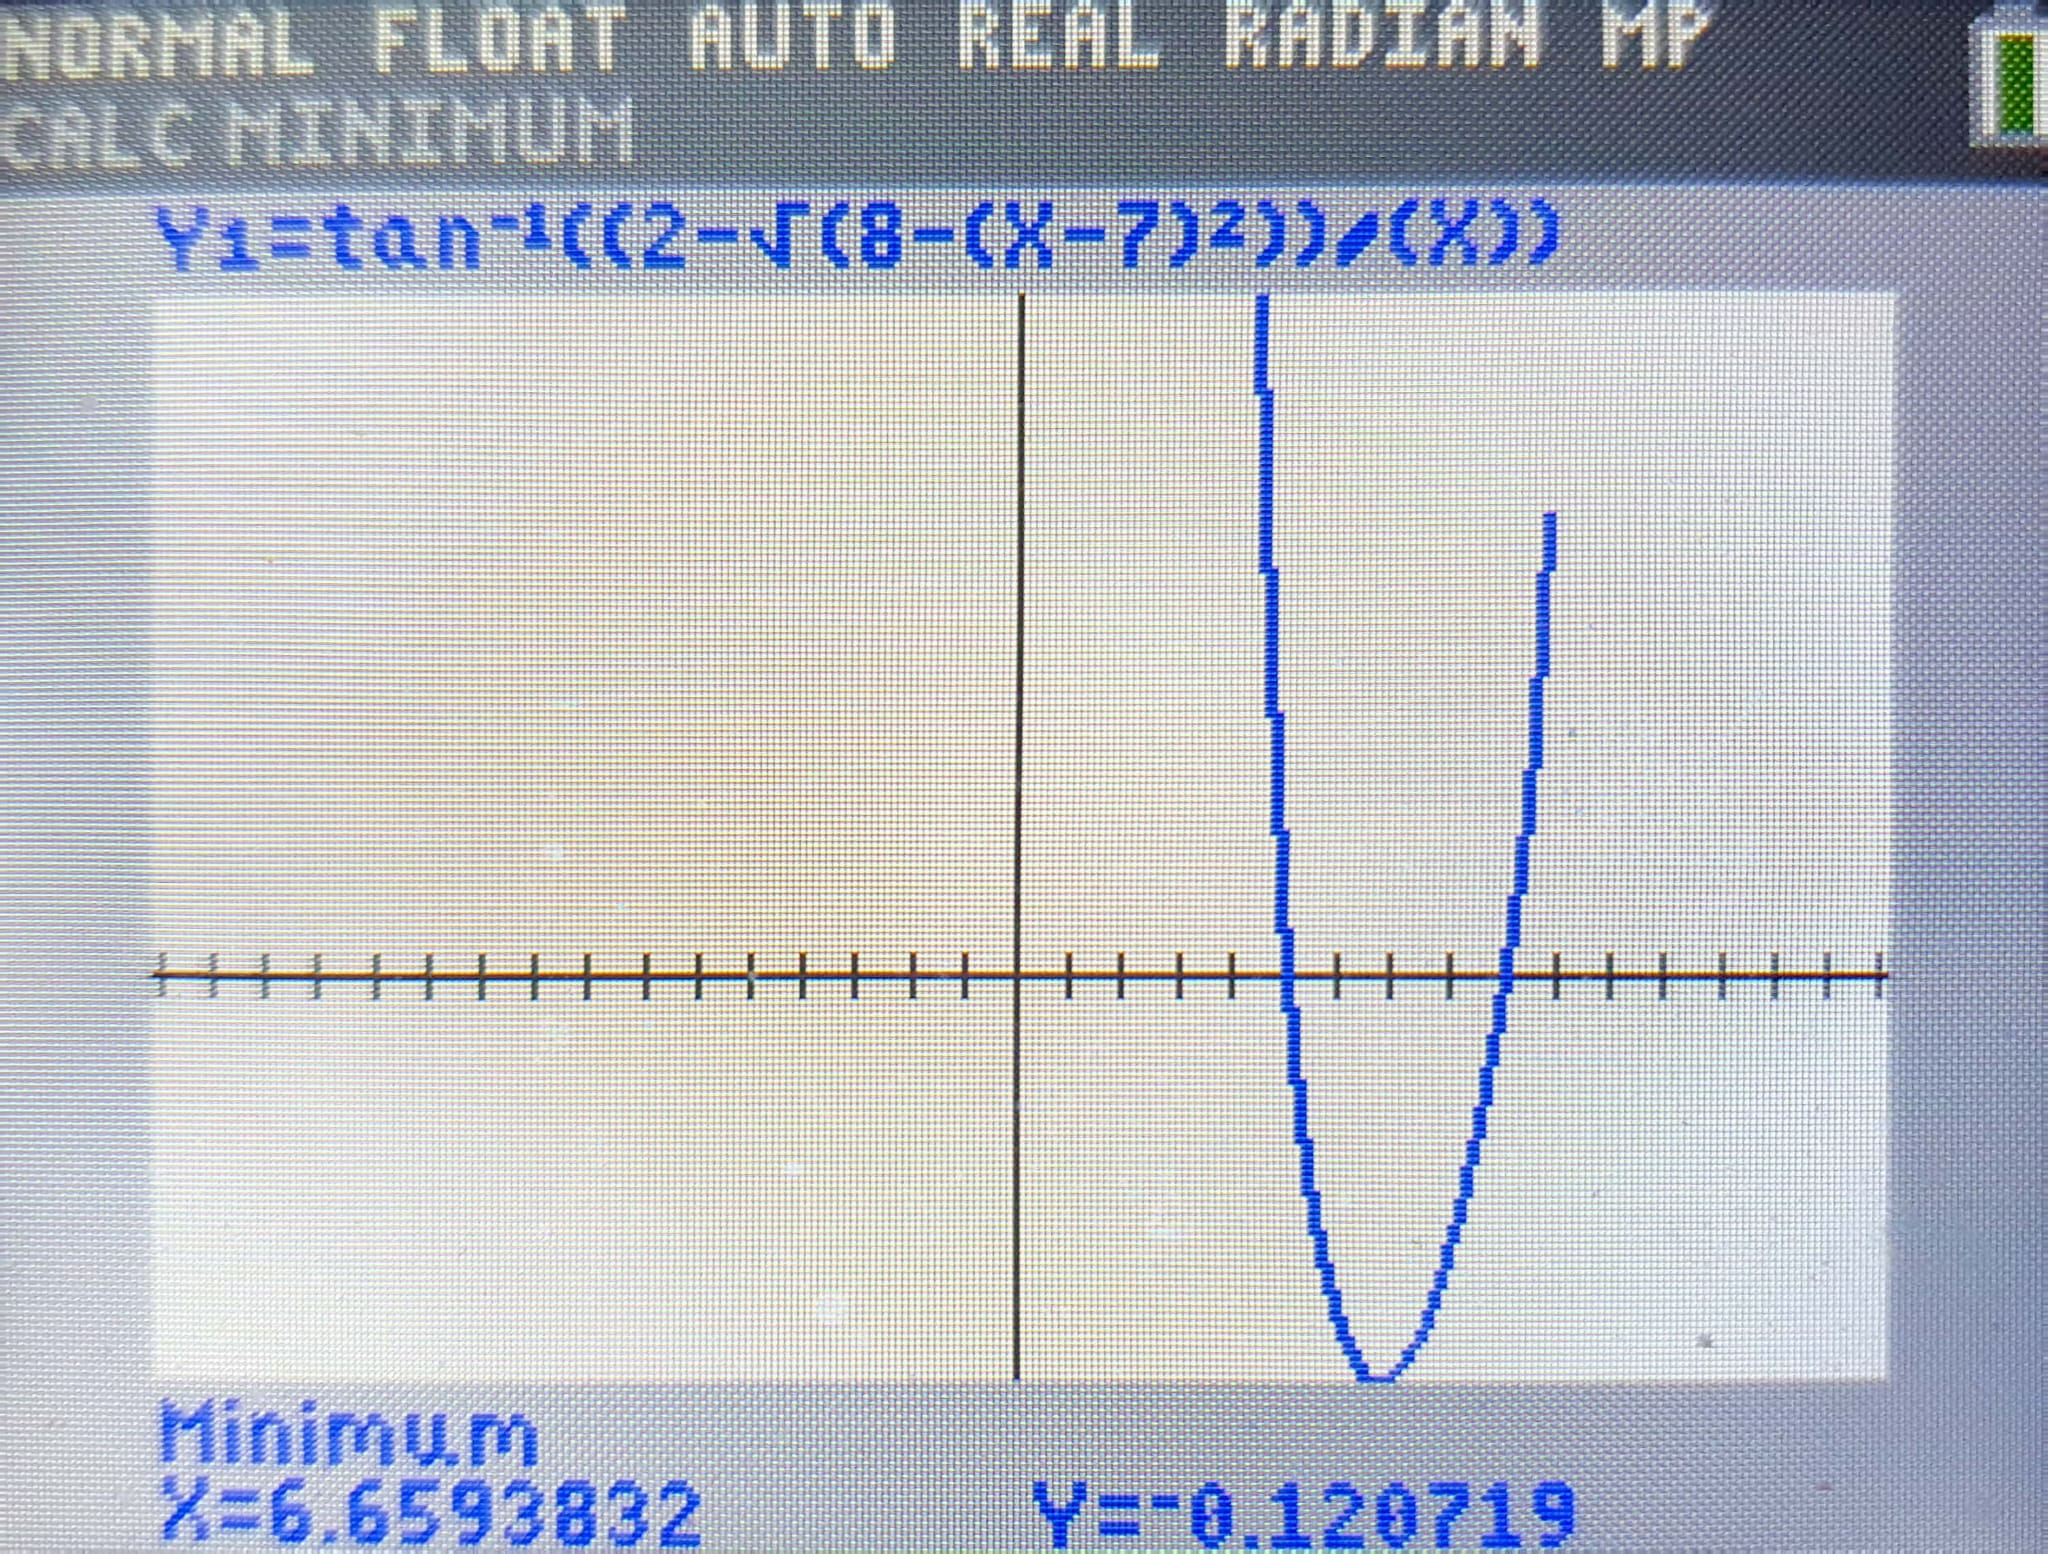
\includegraphics[width=0.5\textwidth]{../images/Complex-Numbers-My-Funnei-Technique.jpg}
        \caption{Brute force technique for finding maximum/minimum angles.}
        \label{fig:brute-force-complex}
      \end{figure}
    \end{enumerate}
  \end{enumerate}
\end{stbox}
\begin{note}
  To show that a \emph{half}-line \(\arg(z-a-bi)=\theta\) meets another loci \(L\), we need to show that 
  \begin{enumerate}[label=(\alph*)]
    \item The line \(y-b=\tan(\theta)(x-a)\) meets the loci \(L\) at some \((u,v)\).
    \item 
    \(\begin{cases}
      u>a &\text{if }\theta\in(-\pi/2,\pi/2),\\
      u=a &\text{if }\theta=\pm\pi/2,\\
      u<a &\text{if }\theta\in(\pi/2,\pi)\cup(-\pi,-\pi/2).
    \end{cases}\)
    \item  
    \(\begin{cases}
      v>b &\text{if }\theta\in(0,\pi),\\
      v=b &\text{if \(\theta=0\) or \(\theta=\pi\)},\\
      v<b &\text{if }\theta\in(-\pi,0).
    \end{cases}\)
  \end{enumerate}
  The latter two conditions must be shown to be clearly satisfied, to illustrate our understanding of \emph{half}-lines. For example, we may write
  \[x=\frac{2-\sqrt{3}}{4}\highlight[yellow]{>-2} \qquad y=\frac{1+10\sqrt{3}}{4}\highlight[yellow]{>1}.\]
\end{note}
\begin{example}{TQ 10(b)}{}
  Show that \(\cot^2(2\pi/5)\) is a root of the equation \(px^2+qx+r=0\), where we are given 
  \[\cot(4\theta)=\frac{\cot^4(\theta)-6\cot^2(\theta)+1}{4\cot^3(\theta)-4\cot(\theta)}.\]
  \rule{20cm-137.0549pt}{0.05mm}
  First notice that \(\cot(8\pi/5)=-\cot(2\pi/5)\). So, 
  \[-\cot(2\pi/5)=\frac{\cot^4(2\pi/5)-6\cot^2(2\pi/5)+1}{4\cot^3(2\pi/5)-4\cot(2\pi/5)}.\]
  Simplifying gives 
  \[5[\cot^2(2\pi/5)]^2-10[\cot^2(2\pi/5)]+1=0.\]
  Thus, \(x=\cot^2(2\pi/5)\) is a root of the equation \(5x^2-10x+1=0\). 
\end{example}
\begin{example}{RV FM 2023 J2 CT}{}
  Show, by using De Moivre's theorem, that provided \(\cos(\theta)\neq 0\), 
  \[\sum_{k=1}^{12}{(-1)^{k-1}\cos((2k-1)\theta)}=\frac{\sin^2(P\theta)}{\cos(\theta)}\]
  where \(P\) is a constant to be determined.

  \rule{20cm-137.0549pt}{0.05mm}

  Let \(C=\sum_{k=1}^{12}{(-1)^{k-1}\cos((2k-1)\theta)}\) and \(S=\sum_{k=1}^{12}{(-1)^{k-1}\sin((2k-1)\theta)}\). Then, for \(z=e^{i\theta}\),
  \begin{align*}
    C+iS &=\sum_{k=1}^{12}{(-1)^{k-1}[\cos((2k-1)\theta)+i\sin((2k-1)\theta)]}\\
    &=\sum_{k=1}^{12}{z(-z^2)^{k-1}}\\
    &=\frac{z\left(1-(-z^2)^{12}\right)}{1-(-z^2)}\\
    &\vdotswithin{=}\\
    &=\frac{-ie^{i(12\theta)}\sin(12\theta)}{\cos(\theta)}.
  \end{align*}
  So, comparing real parts,
  \[C=\frac{(-i)\cdot i\sin(12\theta) \cdot \sin(12\theta)}{\cos(\theta)}=\frac{\sin^2(12\theta)}{\cos(\theta)}.\]
\end{example}
\begin{note}
  Algebraic tricks to know.
  \begin{enumerate}
    \item Factoring out \(e^{i\theta/2}\), given an expression involving \(e^{i\theta}\), can help in simplifying expressions.
    \item Let \(r_1,\dots,r_n\) be the roots of the polynomial \(p(z)\coloneq\sum{a_iz^i}\). To find the sum or product of the roots, consider
    \begin{enumerate*}[itemjoin={, or\ }]
      \item Vieta's Formula
      \item comparing the coefficients of \(p(z)=\highlight[yellow]{a_n}(z-r_1)(z-r_2)\cdots(z-r_n)\).
    \end{enumerate*}
    \item[\(\bigstar\)] Take extra caution to note whether a geometric progression is present.
    \item Let \(n\in \mathbb{Z}^{+}\). Suppose that \(n\) is odd, and we want to express \(\sin^n(\theta)\) as a linear combination of \(\sin(m\theta)\), for \(m\in \mathbb{Z}^{+}\). First notice that \(z^k-\frac{1}{z^k}=2i\sin(k\theta)\), for \(z=e^{i\theta}\). Then, use this fact in conjunction with the binomial theorem:
    \begin{align*}
      \left( z-\frac{1}{z} \right)^n &= \sum_{k=0}^{n}{\binom{n}{k}(-1)^kz^{n-2k}}\\
      [2i\sin(\theta)]^n &= \sum_{k=0}^{\lfloor n/2 \rfloor}{\binom{n}{n-2k}\left( z^{n-2k}-\frac{1}{z^{n-2k}} \right)}.
      % \binom{n}{n}\left( z^n-\frac{1}{z^n} \right)+\binom{n}{n-1}\left( z^{n-2}-\frac{1}{z^{n-2}} \right)+\dots+\binom{n}{\lfloor n/2 \rfloor}\left( z-\frac{1}{z} \right)\\
    \end{align*}
    Comparing imaginary parts, we get \(\sin^n(\theta)\) in the desired form:
    \[\sin^n(\theta)=\frac{1}{2^{n-1}}
    % \left[ \sin(n\theta)+\binom{n}{n-2}\sin((n-2)\theta)+\dots+\binom{n}{\lfloor n/2 \rfloor}\sin(\theta) \right]
    \sum_{k=0}^{\lfloor n/2 \rfloor}{\binom{n}{n-2k}\sin((n-2k)\theta)}.\]
    (Similarly, we can express \(\cos^n(\theta)\) as a linear combination of \(\cos(m\theta)\).)
    \item Now, consider even \(n\), instead. Then, recall that \(z^k+\frac{1}{z^k}=2\cos(k\theta)\). As such,
    \begin{align*}
      [2i\sin(\theta)]^n &= \sum_{k=0}^{n/2}{\binom{n}{n-2k}\left( z^{n-2k}-\frac{1}{z^{n-2k}} \right)}\\
      \sin^n(\theta) &= \frac{1}{2^{n-1}}\sum_{k=0}^{n/2}{\binom{n}{n-2k}\cos((n-2k)\theta)}.
    \end{align*}
    (The case for \(\cos^n(\theta)\) is again similar.)
    % \item Alternatively, we may be asked to express \(\sin(n\theta)\) as a linear combination of \(\sin(m\theta)\), using just De Moivre's theorem. Letting \(c\coloneq\cos(\theta)\) and \(s\coloneq\sin(\theta)\), we first expand
    % \begin{align*}
    %   \cos(n\theta)+i\sin(n\theta) &= [\cos(\theta)+i\sin(\theta)]^n\\
    %   &= \sum_{k=0}^{n}{\binom{n}{k}c^{n-k}i^{k}s^{k}}.
    % \end{align*}
    % Then, compare imaginary parts. (Or real parts, for \(\cos(n\theta)\).)
    \item Let \(n\in \mathbb{Z}^{+}\). Similarly, to find \(\sin(n\theta)\) in terms of powers of \(\sin(\theta)\), first apply De Moivre's theorem:
    \[\cos(n\theta)+i\sin(n\theta)=(c+is)^n=\sum_{k=0}^{n}{\binom{n}{k}c^{n-k}i^ks^k}.\]
    Then, we compare imaginary parts. (Or real parts, for \(\cos(n\theta)\).)
    \item Trigonometric identities:
    \begin{table}[H]
      \centering
      \begin{tabular}{M{0.3\textwidth}M{0.3\textwidth}}
        \toprule
        \(\pi-\theta\) & \(\pi/2-\theta\)\\
        \midrule 
        \(\begin{aligned}
          \sin(\pi-\theta)&=\sin(\theta)\\
          \cos(\pi-\theta)&=-\cos(\theta)\\
          \tan(\pi-\theta)&=-\tan(\theta)
        \end{aligned}\)
        % \begin{itemize}
        %   \item \(\sin(\pi-\theta)=\sin(\theta)\)
        %   \item \(\cos(\pi-\theta)=-\cos(\theta)\) 
        %   \item \(\tan(\pi-\theta)=-\tan(\theta)\)
        % \end{itemize}
        &
        \(\begin{aligned}
          \sin(\pi/2-\theta)&=\cos(\theta)\\
          \cos(\pi/2-\theta)&=\sin(\theta)\\
          \tan(\pi/2-\theta)&=\cot(\theta)
        \end{aligned}\)\\
        % \begin{itemize}
        %   \item \(\sin(\pi/2-\theta)=\cos(\theta)\)
        %   \item \(\cos(\pi/2-\theta)=\sin(\theta)\)
        %   \item \(\tan(\pi/2-\theta)=\cot(\theta)\)
        % \end{itemize}\\
        \bottomrule
      \end{tabular}
      \caption{}
      \label{table:trigonometric-identities}
    \end{table}
    \item Let \(z^n=1\). Then, \(\sum{z^i}=z^n\sum{z^i}=\sum{z^{n+i}}\).
    \item When asked to prove an identity involving binomial coefficients \(\binom{n}{k}\), try to factor the given form using the binomial theorem. 
  \end{enumerate}
\end{note}
\begin{example}{Algebraic tricks to know}{}
  \begin{enumerate}
    \item[1(a).] Simplifying a complex number \(w\) to a given form. 
    \begin{align*}
      w&=\frac{-ie^{2ki\pi/5}}{1-e^{2ki\pi/5}}=\frac{-ie^{2ki\pi/5}}{e^{ki\pi/5}\left[ e^{-ki\pi/5}-e^{ki\pi/5} \right]}=\frac{-ie^{ki\pi/5}}{-2i\sin(k\pi/5)}\\
      &=\frac{\cos(k\pi/5)+i\sin(k\pi/5)}{2\sin(k\pi/5)}=\frac{1}{2}[\cot(k\pi/5)+i]
    \end{align*}
    \item[1(b).]
    \[z=2\left( 1+e^{2ki\pi/3} \right)=2e^{ki\pi/3}\left( e^{-ki\pi/3}+e^{ki\pi/3} \right)=4\cos(k\pi/3)e^{ki\pi/3}.\]
    \item[1(c).] Let \(z_k=e^{2ki\pi/n}\) for all \(1\leq k\leq n\). In the case where \(n\) is odd, i.e. \(n=2m+1\), evaluate the series \(\sum_{k=1}^{n}{2(1+z_k)^{-1}}\).
    \begin{align*}
      \sum_{k=1}^{n}{\frac{2}{1+z_k}}&=\sum_{k=1}^{n}{\frac{2}{1+e^{2ki\pi/n}}}=\sum_{k=1}^{n}{\frac{2}{e^{ki\pi/n}\left( e^{-ki\pi/n}+e^{ki\pi/n} \right)}}=\sum_{k=1}^{n}{\frac{2e^{-ki\pi/n}}{2\cos(k\pi/n)}}\\
      &=\sum{k=1}^{n}\frac{\cos(k\pi/n)-i\sin(k\pi/n)}{\cos(k\pi/n)}=\sum_{k=1}^{n}{1-i\tan(k\pi/n)}\\
      &=n-i\Bigl[\bigl[\tan(\pi/n)+\tan((n-1)\pi/n)\bigr]+\bigl[\tan(2\pi/n)+\tan((n-2)\pi/n)\bigr]+...\\
      &\hphantom{={}}+\bigl[\tan(m\pi/n)+\tan((n-m)\pi/n)\bigr]+\tan(\pi)\Bigr]\\
      &=n+i(0+0+\dots+0)=n
    \end{align*}
    because \(\tan(\pi-\theta)=-\tan(\theta)\).
    \item[2.] We found that the roots of \((1+z)^4+(1-z)^4=0\) has roots \(i\tan(k\pi/8)\), where \(k=1,3,4,7\). Then, we were tasked to find the value of \(\tan^2(\pi/8)+\tan^2(3\pi/8)\) and \(\tan^2(5\pi/8)\tan^2(\pi/8)\tan^2(3\pi/8)\).\\[\baselineskip]
    Since \(\tan(\pi/8)=-\tan(7\pi/8)\) and \(\tan(3\pi/8)=-\tan(5\pi/8)\),
    \begin{align*}
      (1+z)^4+(1-z)^4 &= \highlight[yellow]{2}[z-i\tan(\pi/8)][z+i\tan(\pi/8)][z-i\tan(3\pi/8)][z+i\tan(3\pi/8)]\\
      &= \highlight[yellow]{2}[z^2+\tan^2(\pi/8)][z^2+\tan^2(3\pi/8)].
    \end{align*}
    Comparing constants/coefficients of \(z^2\), we obtain 
    \[\tan^2(\pi/8)\tan^2(3\pi/8)=1 \qquad\text{and}\qquad \tan^2(\pi/8)+\tan^2(3\pi/8)=6,\]
    respectively.  
    \item[3.] The case of \(n=5\): expressing \(\sin^5(\theta)\), in terms of \(\sin(m\theta)\).
    \begin{align*}
      \left( z-\frac{1}{z} \right)^5 &= z^5-5z^3+10z-\frac{10}{z}+\frac{5}{z^3}-\frac{1}{z^5}\\
      [2i\sin(\theta)]^5 &= \left( z^5-\frac{1}{z^5} \right)-5\left( z^3-\frac{1}{z^3} \right)+10\left( z-\frac{1}{z} \right)\\
      32i\sin^5(\theta) &= 2\sin(5\theta)-5(2)i\sin(3\theta)+10(2)i\sin(\theta)\\
      \sin^5(\theta) &= \frac{1}{16}\sin(5\theta)-\frac{5}{16}\sin(3\theta)+\frac{5}{8}\sin(\theta).
    \end{align*}
    \setcounter{enumi}{6}
    \item Let \(\omega=e^{2i\pi/11}\). We define
    \[\alpha=\omega+\omega^3+\omega^4+\omega^5+\omega^9 \qquad\text{and}\qquad \beta=\omega^{-1}+\omega^{-3}+\omega^{-4}+\omega^{-5}+\omega^{-9}.\]
    Find \((x-\alpha)(x-\beta)\) in its simplest form. Notice that \(\beta=\omega^{11}\beta=\omega^{10}+\omega^8+\omega^7+\omega^6+\omega^2\). As such,
    \[\alpha+\beta=\sum_{k=1}^{10}{\omega^k}=-1 \qquad\text{and}\qquad \alpha\beta=\underbrace{5+2\left( \sum_{k=1}^{10}{\omega^k} \right)}_{\text{the usual expansion}}=5-2=3.\]
    Now, \((x-\alpha)(x-\beta)=x^2-(\alpha+\beta)x+\alpha\beta=x^2+x+3\).
    \item Let 
    \begin{align*}
      C&=1-\binom{2n}{1}\cos(\theta)+\binom{2n}{2}\cos(2\theta)-\binom{2n}{3}\cos(3\theta)+\dots+\cos(2n\theta)\\
      S&=-\binom{2n}{1}\sin(\theta)+\binom{2n}{2}\sin(2\theta)-\binom{2n}{3}\sin(3\theta)+\dots+\sin(2n\theta),
    \end{align*}
    where \(n\) is a positive integer. Then, 
    \begin{align*}
      C+iS&=\sum_{r=0}^{2n}{(-1)^r\binom{2n}{r}[\cos(r\theta)+i\sin(r\theta)]}\\
      &=\sum_{r=0}^{2n}{\binom{2n}{r}(-1)^re^{i(r\theta)}}=\sum_{r=0}^{2n}{\binom{2n}{r}(1)^{2n-r}\left( -e^{i\theta} \right)^r}\\
      &=\left(1-e^{i\theta}\right)^{2n}=\left( e^{i\theta/2} \right)^{2n}\left( e^{-i\theta/2}-e^{i\theta/2} \right)^{2n}\\
      &=e^{in\theta}[-2i\sin(\theta/2)]^{2n}\\
      &=(-4)[\cos(n\theta)+i\sin(n\theta)]\sin^{2n}(\theta/2).
    \end{align*}
    Comparing real and imaginary parts,
    \[C=(-4)^n\cos(n\theta)\sin^{2n}(\theta/2) \qquad\text{and}\qquad S=(-4)^n\sin(n\theta)\sin^{2n}(\theta/2).\]
  \end{enumerate}
\end{example}
\begin{note}
  Geometrical tricks to know.
  \begin{enumerate}
    \item Where clarity may otherwise be lacking, consider making a line segment \emph{thicker} and \emph{label} it with ``\textrightarrow\ required points'' --- to indicate that it is the locus being requested for.  
    \item Be aware of any triangles, congruent triangles, common angles, and sides of common length. In particular, when a triangle has an angle of \(\pi/4=45^{\circ}\), it is an isosceles triangle. These observations are especially helpful in finding circle-line intersections.
  \end{enumerate}
\end{note}
\begin{example}{}{}
  \begin{figure}[H]
    \centering
    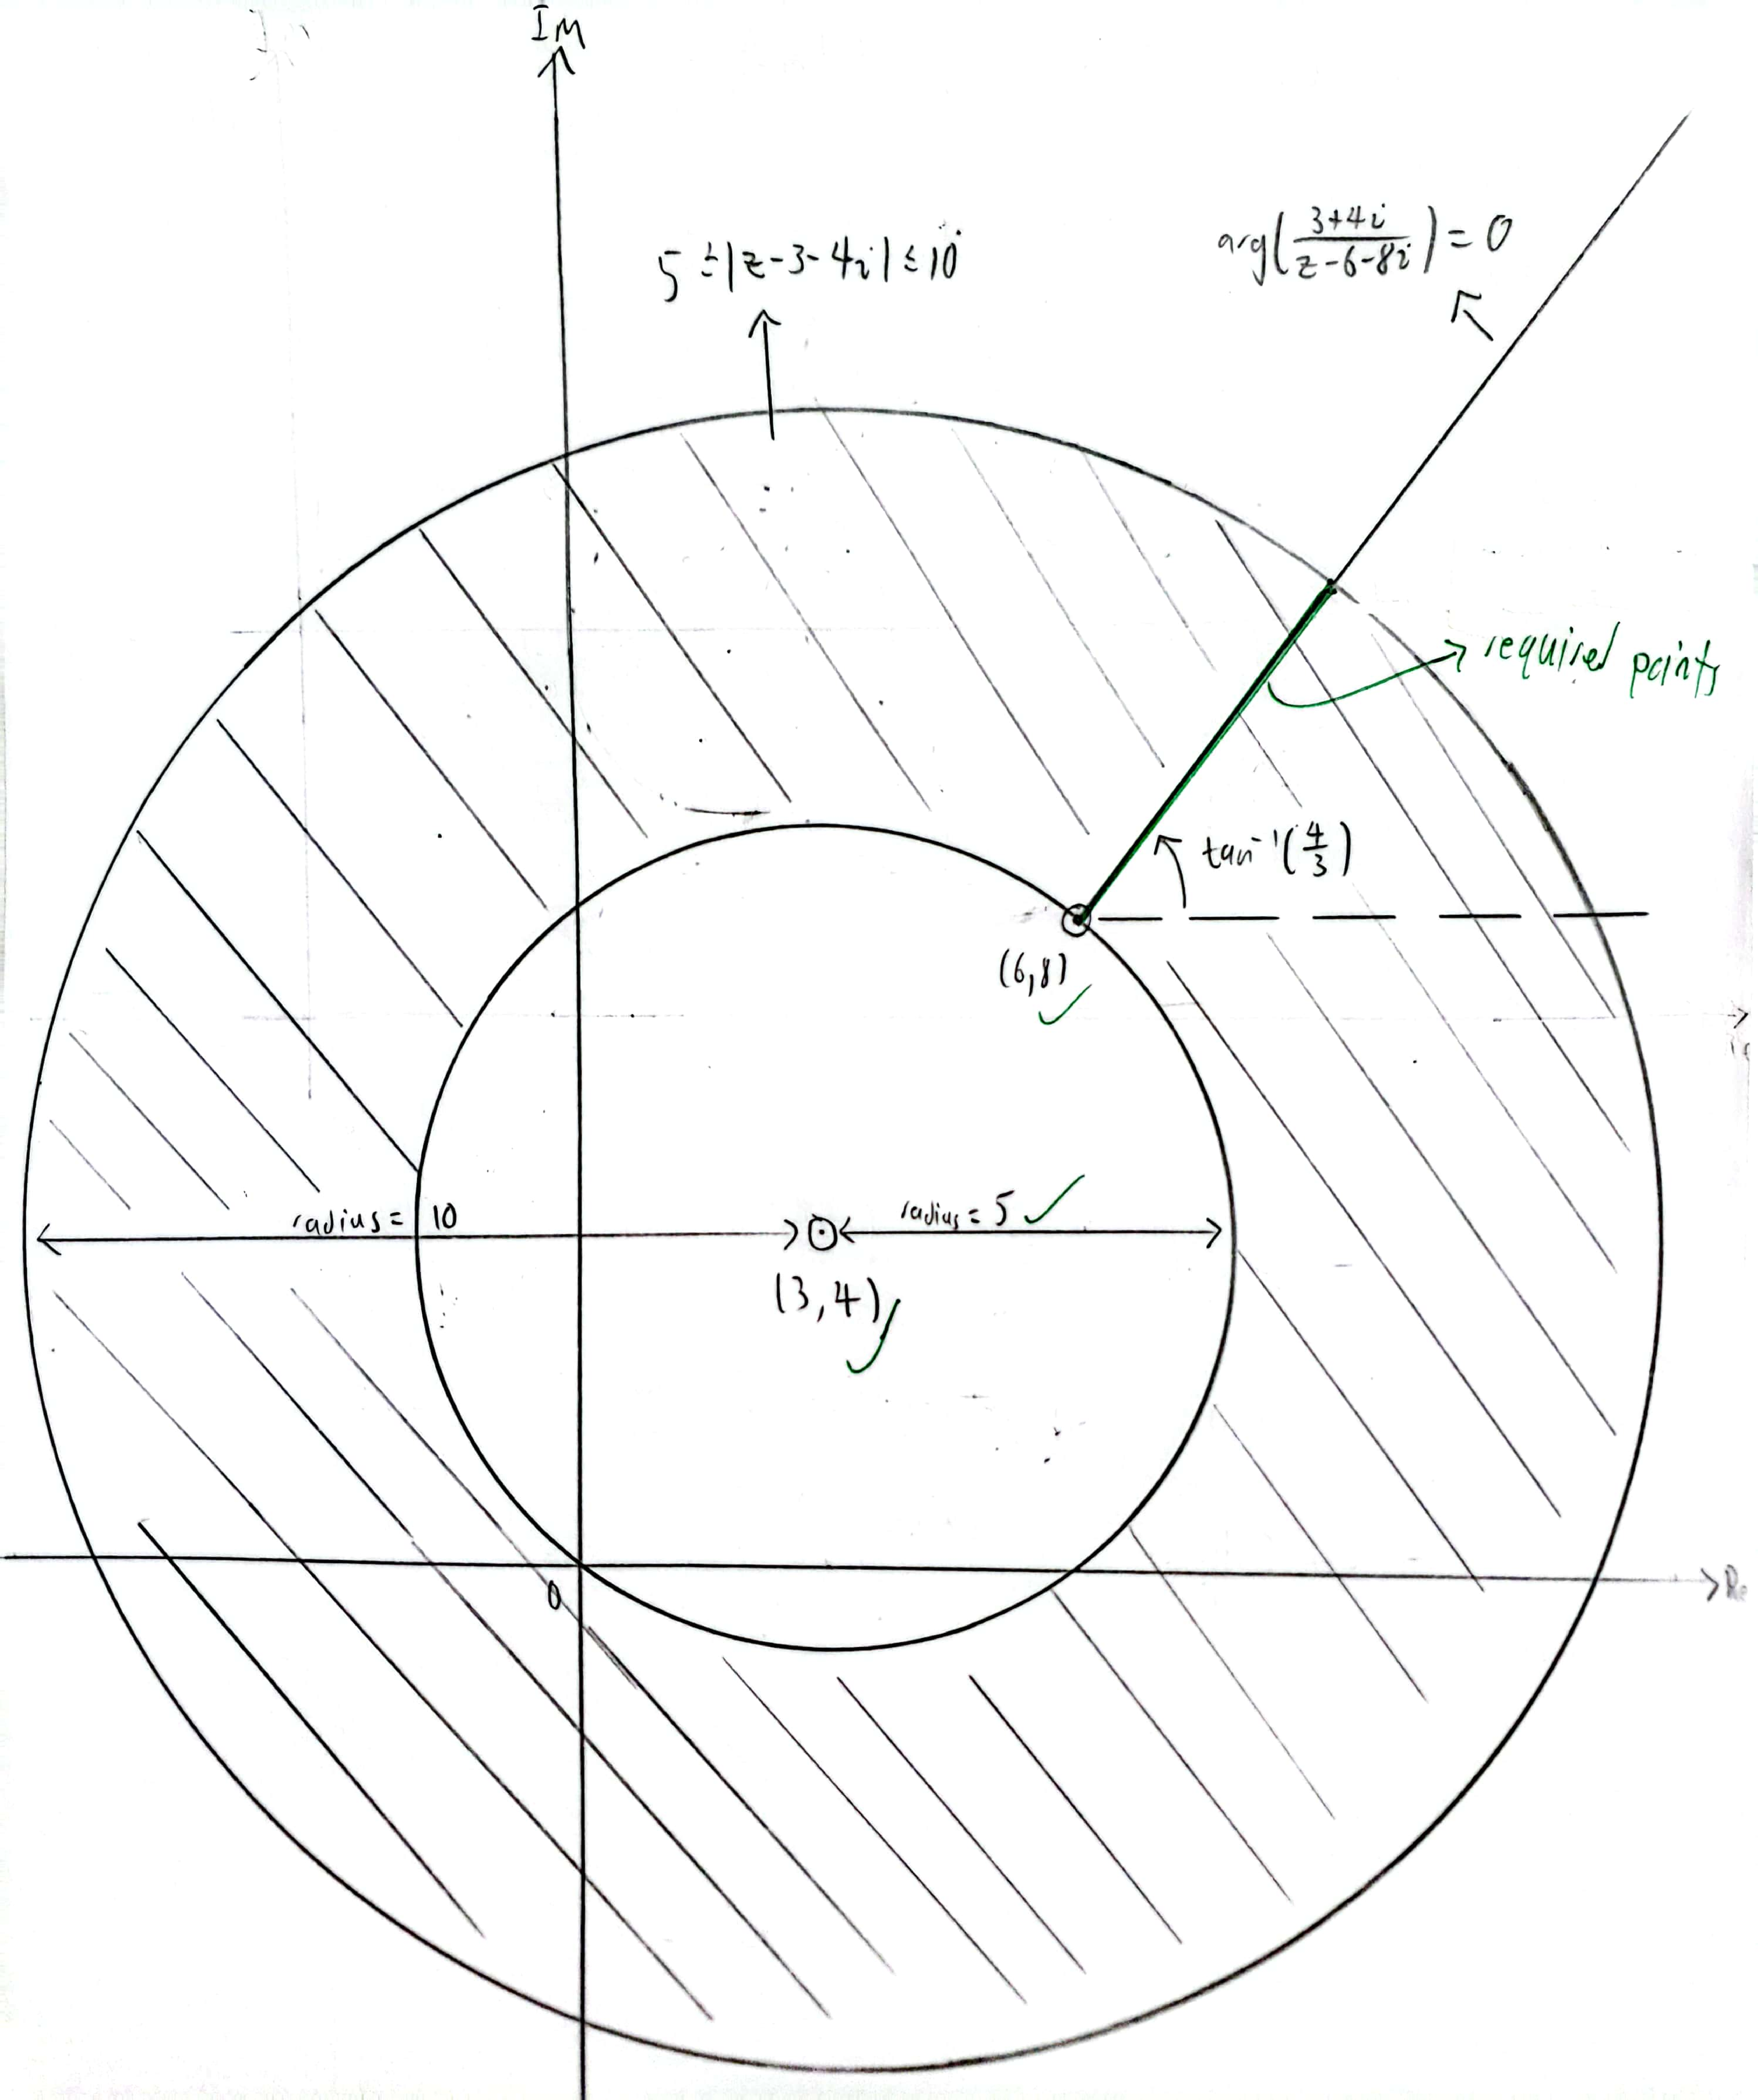
\includegraphics[width=0.6\textwidth,page=1]{../Diagrams/Complex-revision.pdf}
    \caption{\ref{Me} \textcolor{green!85!black}{Annotations} that improve clarity.}
    \label{fig:complex-clarity-improvements}
  \end{figure}
  \begin{figure}[H]
    \centering
    \begin{subfigure}[c]{0.45\textwidth}
      \centering
      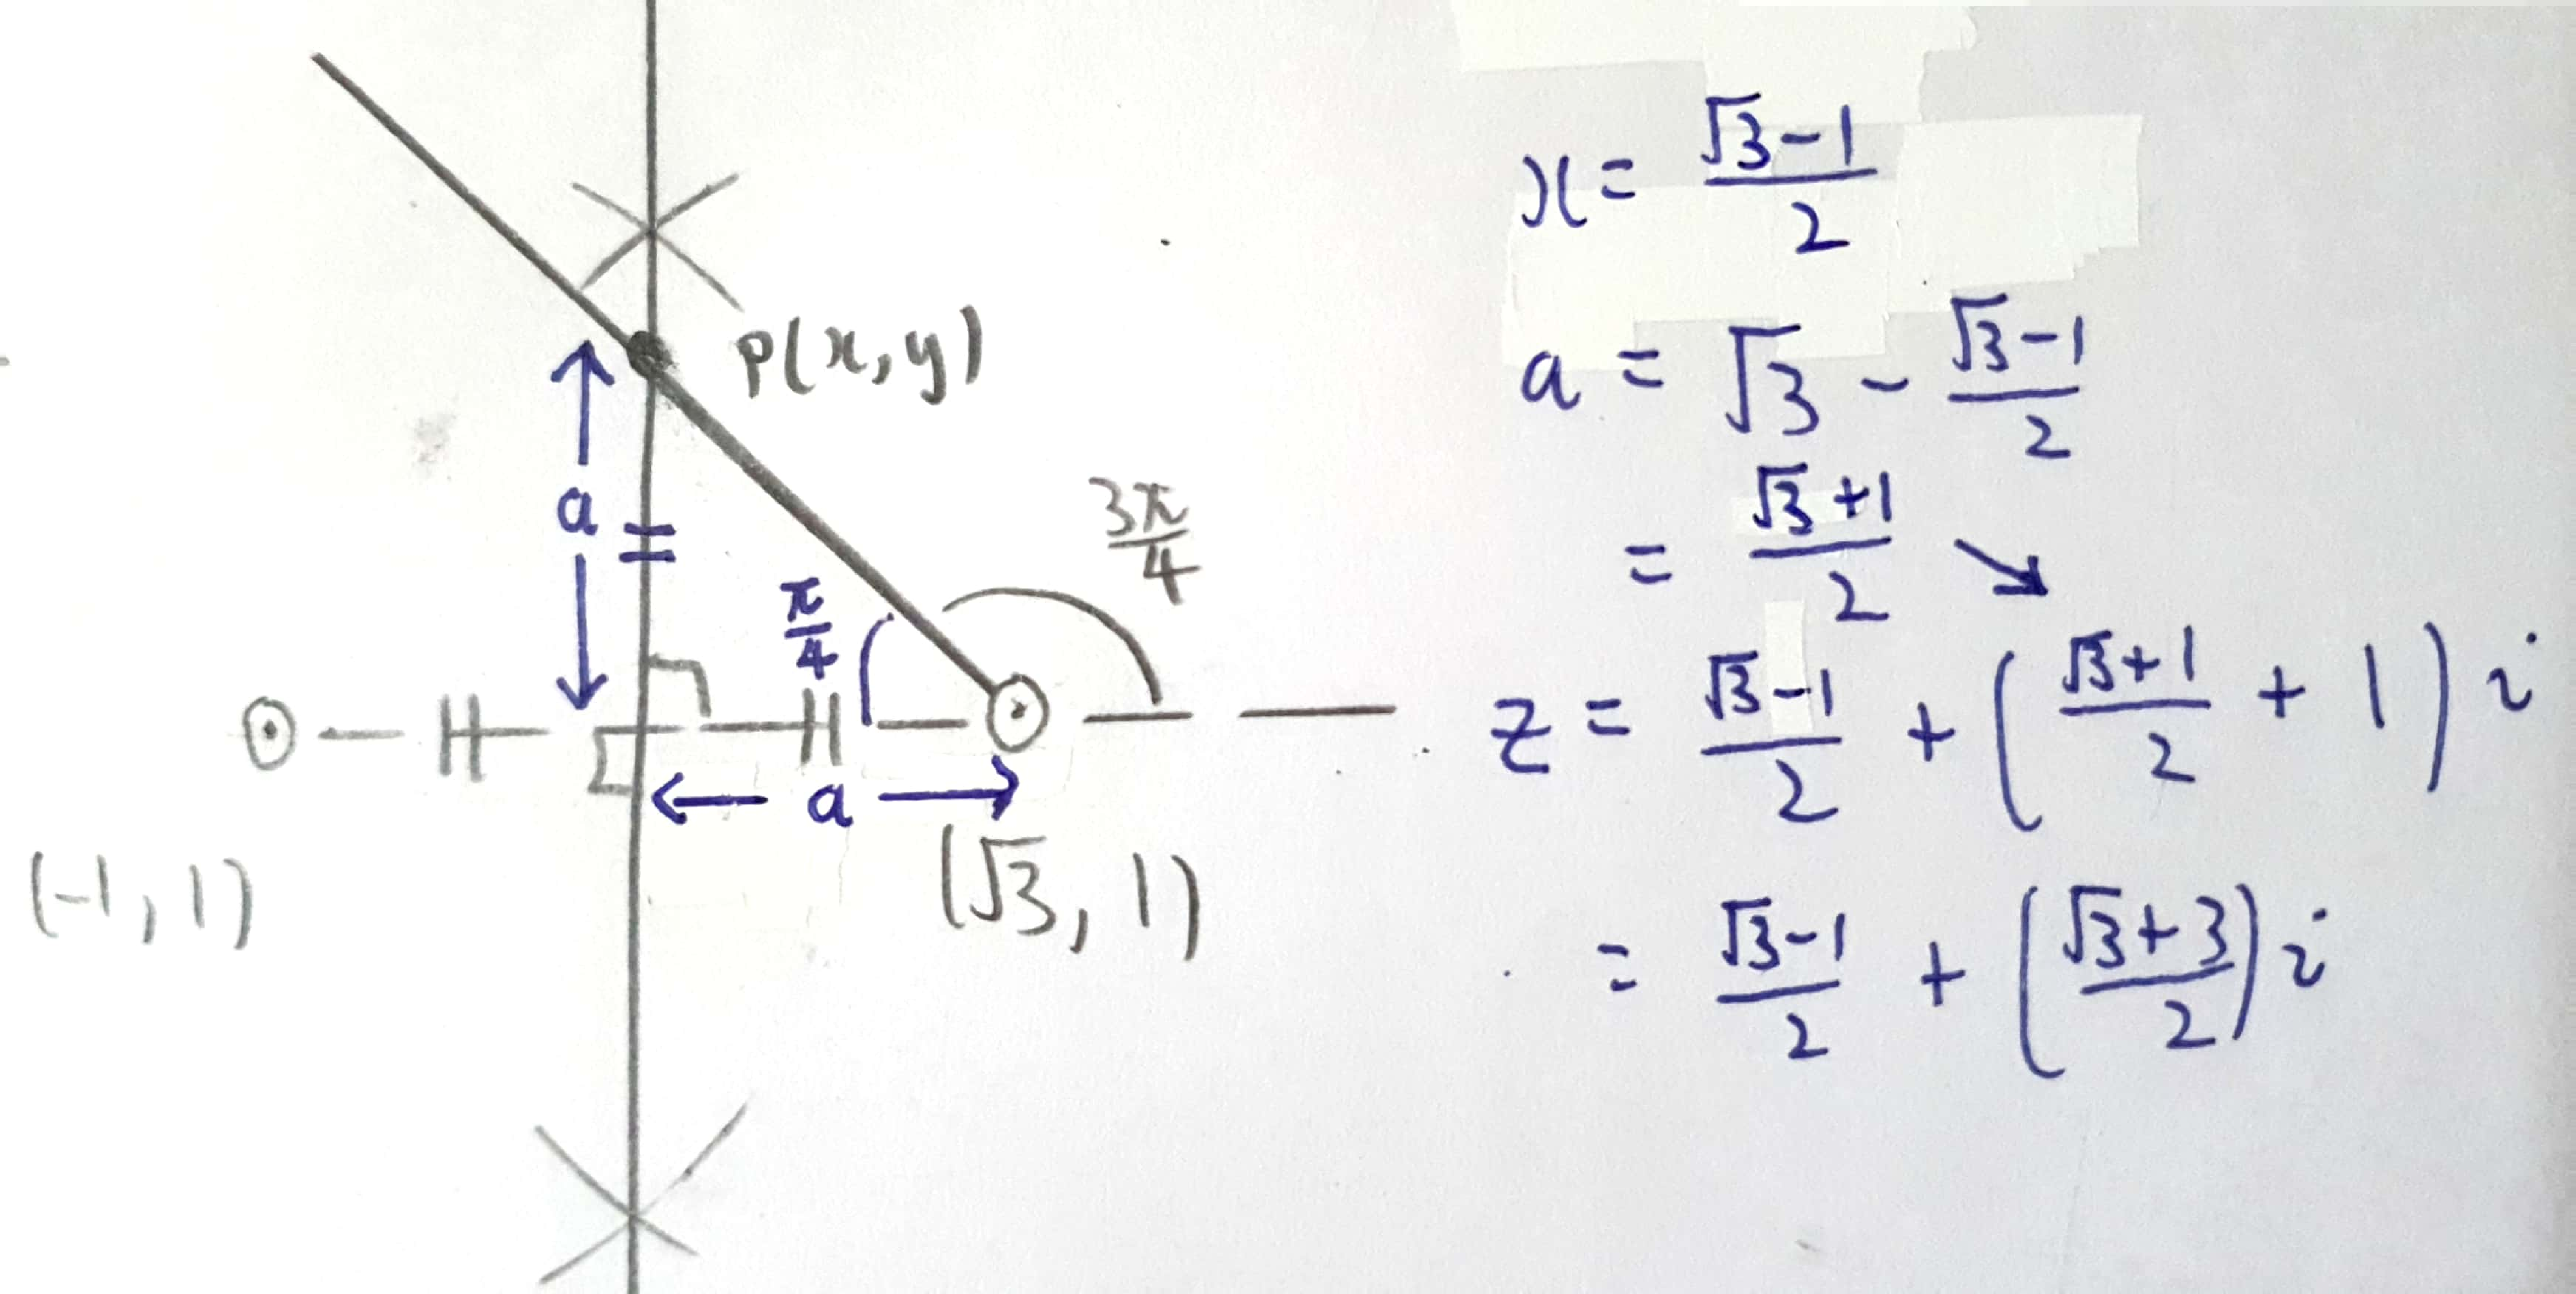
\includegraphics[width=\textwidth,page=1]{../Diagrams/FM-CT-2024-Q5.pdf}
      \caption{Finding the intersection of the two lines.}
  \end{subfigure}\hfill
  \begin{subfigure}[c]{0.45\textwidth}
      \centering
      \includegraphics[width=\textwidth,page=2]{../Diagrams/FM-CT-2024-Q5.pdf}
      \caption{Finding the radius \(R\) for which the circle just touches the half-line.}
  \end{subfigure}

  \begin{subfigure}[c]{0.45\textwidth}
    \centering
    \includegraphics[width=\textwidth,page=3]{../Diagrams/Complex-revision.pdf}
    \caption{Finding the shortest distance \(L\) and \(D\) of \((2,-\sqrt{3})\), from the circle and line, respectively.}
  \end{subfigure}
    \caption{\ref{Me} The \textcolor{blue}{writing in blue} denote the deductions we should make.}
    \label{fig:RVFM-CT-2024-Complex}
  \end{figure}
\end{example}
\chapter{Linear Algebra}
\section{Vector spaces, subspaces, linear combinations, bases, linear transformations}
\begin{definition}{}{}
    A vector space (or linear space) \(V\) over a field \(\mathbb{F}\) consists of a set on which two operations (called addition and multiplication respectively here) are defined so that;
\begin{itemize}[label=(M1),leftmargin=*]
    \item[(A)](\(V\) is Closed Under Addition) For all \(\mathbf{x},\mathbf{y} \in V\), there exists a unique element \(\mathbf{x}+\mathbf{y} \in V\).
    \item[(M)](\(V\) is Closed Under Scalar Multiplication) For all elements \(a \in \mathbb{F}\) and elements \(\mathbf{x} \in V\), there exists a unique element \(a\mathbf{x} \in V\).
\end{itemize}
Such that the following properties hold:  
\begin{enumerate}[label=(VS {{\arabic*}}), leftmargin=*]
    \item \label{(VS 1)}(Commutativity of Addition) For all \(\mathbf{x},\mathbf{y} \in V\), we have \(\mathbf{x}+\mathbf{y}=\mathbf{y}+\mathbf{x}\).
    \item \label{(VS 2)}(Associativity of Addition) For all \(\mathbf{x},\mathbf{y},\mathbf{z} \in V\), we have \((\mathbf{x}+\mathbf{y})+\mathbf{z}=\mathbf{x}+(\mathbf{y}+\mathbf{z})\).
    \item \label{(VS 3)}(Existance of The Zero/Null Vector) There exists an element in \(V\) denoted by \({\mathbf{0}}\), such that \(\mathbf{x}+{\mathbf{0}}=\mathbf{x}\) for all \(\mathbf{x} \in V\).
    \item \label{(VS 4)}(Existance of Additive Inverses) For all elements \(\mathbf{x} \in V\), there exists an element \(\mathbf{y} \in V\) such that \(\mathbf{x}+\mathbf{y}={\mathbf{0}}\).
    \item \label{(VS 5)}(Multiplicative Identity) For all elements \(x \in V\), we have \(1\mathbf{x}=\mathbf{x}\), where 1 denotes the multiplicative identity in \(\mathbb{F}\).
    \item \label{(VS 6)}(Compatibility of Scalar Multiplication with Field Multiplication) For all elements \(a,b \in \mathbb{F}\) and elements \(\mathbf{x} \in V\), we have \((ab)\mathbf{x}=a(b\mathbf{x})\).
    \item \label{(VS 7)}(Distributivity of Scalar Multiplication over Vector Addition) For all elements \(a \in \mathbb{F}\) and elements \(\mathbf{x},\mathbf{y} \in V\), we have \(a(\mathbf{x}+\mathbf{y})=a\mathbf{x}+a\mathbf{y}\).
    \item \label{(VS 8)}(Distributivity of Scalar Multiplication over Field Addition) For all elements \(a,b \in \mathbb{F}\), and elements \(\mathbf{x} \in V\), we have \((a+b)\mathbf{x}=a\mathbf{x}+b\mathbf{x}\).
\end{enumerate}
\end{definition}
\begin{theorem}{}{}
    Let \(V\) be a vector space and \(W\) a subset of \(V\). Then \(W\) is a subspace of \(V\) iff the following 3 conditions hold for the operations defined in V.
            \begin{enumerate}[label=(\alph*)]
                \item \(\mathbf{0} \in W\) \label{Theorem 1.3(a)}
                \item \(\mathbf{x}+\mathbf{y} \in W\) whenever \(\mathbf{x} \in W\) and \(\mathbf{y} \in W\). \label{Theorem 1.3(b)}
                \item \(c\mathbf{x} \in W\) whenever \(c \in \mathbb{F}\) and \(\mathbf{x} \in W\). \label{Theorem 1.3(c)}
            \end{enumerate}
\end{theorem}
\begin{definition}{}{}
    A subset \(S\) of a vector space \(V\) \emph{generates} (or \emph{spans}) \(V\) iff \(\Span(S)=V\). In this case, we also say that the vectors of \(S\) generate (or span) \(V\).
\end{definition}
\begin{definition}{}{}
    Let \(V\) be a vector space and \(S\) a nonempty subset of \(V\). A vector \(v \in V\) is called a \emph{linear combination} of vectors of \(S\) iff there exists a finite number of vectors \(\mathbf{u}_1,\mathbf{u}_2,\dots,\mathbf{u}_n\) in \(S\) and scalars \(a_1,a_2,\dots,a_n\) in \(\mathbb{F}\) such that
            \[v=\sum_{i=1}^{n}{a_i\mathbf{u}_i}.\]
            In this case we also say that \(v\) is a linear combination of \(\mathbf{u}_1,\mathbf{u}_2,\dots,\mathbf{u}_n\) and call \(a_1,a_2,\dots,a_n\) the \emph{coefficients} of the linear combination
\end{definition}
\begin{definition}{}{}
    A set subset \(S\) of a vector space \(V\) is called \emph{linearly dependent} iff there exists a finite number of distinct vectors \(\mathbf{u}_1,\mathbf{u}_2,\dots,\mathbf{u}_n\)in \(S\) and scalars \(a_1,a_2,\dots,a_n\) not all zero, such that
            \[a_1\mathbf{u}_1+a_2\mathbf{u}_2+a_n\mathbf{u}_n=\mathbf{0}.\]
\end{definition}
\begin{definition}{}{}
    A \emph{basis} \(\beta\) for a vector space \(V\) is a linearly independent subset of \(V\) that generates \(V\). If \(\beta\) is a basis for \(V\), we also say that the vectors of \(\beta\) form a basis for \(V\).
\end{definition}
\begin{definition}{}{}
    Let \(V\) and \(W\) be vector spaces. We call a function \(T\colon V\to W\) a \emph{linear transformation from \(V\) to \(W\)} iff \(T(c\mathbf{x}+\mathbf{y})=cT(\mathbf{x})+T(\mathbf{y})\) for all \(\mathbf{x},\mathbf{y}\in V\) and \(c\in \mathbb{F}\).
\end{definition}
\begin{theorem}{The Rank-Nullity Theorem.}{}
    For any vector spaces \(V\) and \(W\), and a linear transformation \(T \colon V \to W\), it holds that
    \[\rank(T)+\nullity(T)=\dim(V).\]
\end{theorem}
\section{Matrices and systems of linear equations}
\begin{stbox}{General Information}
    \begin{itemize}
        \item Let \(\mathbf{A}\) be an \(m\times n\) matrix, and \(\mathbf{a}_j\) its \(j\)th column. For any \(\mathbf{x}=
        \begin{pmatrix}
            x_1 & x_2 & \cdots & x_n\\
        \end{pmatrix}^\top\), 
        \[\mathbf{A}\mathbf{x}=\sum_{j=1}^{n}{x_j}\mathbf{a}_j.\]
        \item Let \(\mathbf{A}\) and \(\mathbf{B}\) be matrices having \(n\) rows. For any matrix \(\mathbf{M}\) with \(n\) columns, we have
        \[\mathbf{M}
        \begin{pNiceArray}{c|c}
            \mathbf{A} & \mathbf{B}
        \end{pNiceArray}=
        \begin{pNiceArray}{c|c}
            \mathbf{M}\mathbf{A} & \mathbf{M}\mathbf{B}
        \end{pNiceArray}.\]
    \end{itemize}
\end{stbox}
\begin{definition}{}{}
    A system \(\mathbf{A}\mathbf{x}=\mathbf{b}\) is \emph{homogeneous} iff \(\mathbf{b}=0\); otherwise it is \emph{nonhomogeneous}.
\end{definition}
\begin{theorem}{}{}
    For any matrix, its row space, column space, and rank are identical.
\end{theorem}
\begin{theorem}{}{}
    A system \(\mathbf{A}\mathbf{x}=\mathbf{0}\) of \(m\) linear equations in \(n\) unknowns has a solution space of dimension \(n-\rank(A)\).
\end{theorem}
\begin{definition}{}{}
    A system \(\mathbf{A}\mathbf{x}=\mathbf{b}\) of linear equations is \emph{consistent} iff its solution set is nonempty; otherwise it is \emph{inconsistent}.
\end{definition}
\begin{theorem}{The Rouché-Capelli Theorem.}{}
    A system \(\mathbf{A}\mathbf{x}=\mathbf{b}\) is consistent iff \(\rank(\mathbf{A})=\rank(\mathbf{A}\vert \mathbf{b})\).
\end{theorem}
\begin{definition}{}{}
    A matrix is said to be in \emph{reduced row echelon form} iff
        \begin{itemize}
            \item Any row containing a nonzero entry precedes any row in which all the entries are zero (if any).
            \item The first nonzero entry in each row is the only nonzero entry in its column.
            \item The first nonzero entry in each row is 1 and it occurs in a column to the right of the first nonzero entry in the preceding row.
        \end{itemize}
\end{definition}
\begin{stbox}{General Information}
    \begin{itemize}
        \item Gaussian elimination. 
        \begin{itemize}
            \item In the forward pass, the augmented matrix is transformed into an upper triangular matrix in which the first nonzero entry of each row is 1 and it occurs in a column to the right of the first nonzero entry
            of each preceding row.
            \item  In the backward pass, the upper triangular matrix is transformed into reduced row echelon form by making the first nonzero entry of each row the only nonzero entry of its column.
        \end{itemize}
        \item Gaussian elimination always reduces a matrix to its rref form.
        \item Gaussian elimination always reduces \((\mathbf{A} \,\vert\, \mathbf{I}_n)\to (\mathbf{I}_n \,\vert\, \mathbf{A}^{-1})\).
        \item Let \(\mathbf{A}\coloneq
        \begin{pmatrix}
            \mathbf{a}_1&\mathbf{a}_2&\cdots&\mathbf{a}_n
        \end{pmatrix}\) be \(m\times n\) matrix, and \(\mathbf{A}'\coloneq
        \begin{pmatrix}
            \mathbf{a}'_1&\mathbf{a}'_2&\cdots&\mathbf{a}'_n
        \end{pmatrix}\) its rref. Then, \(\{\mathbf{a}_{k_1},\mathbf{a}_{k_2},\dots,\mathbf{a}_{k_m}\}\) is linearly independent iff \(\{\mathbf{a}'_{k_1},\mathbf{a}'_{k_2},\dots,\mathbf{a}'_{k_m}\}\) is. Moreover, the row space of \(\mathbf{A}\) and \(\mathbf{A}'\) are clearly identical.
        \item \href{https://math.stackexchange.com/a/802878}{(Example)} To find a basis for the intersection of the column spaces of \(\mathbf{A},\mathbf{B}\in\MS_{n \times n}(\mathbb{F})\), we reduce
        \[\begin{pmatrix}
            \mathbf{A}&\mathbf{B}
        \end{pmatrix}\to
        \begin{pmatrix}
            \mathbf{A'}&\mathbf{B'}
        \end{pmatrix}.\]
        Let \(\mathbf{c}_i\) and \(\mathbf{c'}_i\) be the \(i\)th columns of 
        \(\begin{pmatrix}
            \mathbf{A}&\mathbf{B}
        \end{pmatrix}\) and
        \(\begin{pmatrix}
            \mathbf{A'}&\mathbf{B'}
        \end{pmatrix}\), respectively.
        We compare the columns of \(\mathbf{A'}\) and \(\mathbf{B'}\) to find a basis \(\beta'\coloneq\{\mathbf{c}'_{i_1},\mathbf{c}'_{i_2},\dots,\mathbf{c}'_{i_r}\}\) for the intersection of the column spaces of \(\mathbf{A'}\) and \(\mathbf{B'}\). Then, \(\beta\coloneq\{\mathbf{c}_{i_1},\mathbf{c}_{i_2},\dots,\mathbf{c}_{i_r}\}\) is a basis for the intersection of the column spaces of \(\mathbf{A}\) and \(\mathbf{B}\).
        % \begin{enumerate}
        %     \item First notice that \(\mathbf{v} \in V\cap W\) iff
        %     \[\mathbf{v}=\mathbf{A}\mathbf{x}_1=\mathbf{B}\mathbf{x}_2\]
        %     for some \(\mathbf{x}_2\in \mathbb{F}^m\) and \(\mathbf{x}_2\in \mathbb{F}^k\). That is,
        %     \[\begin{pmatrix}
        %         \mathbf{A} & \mathbf{B} 
        %     \end{pmatrix}
        %     \begin{pmatrix}
        %         \mathbf{x_1}\\
        %         -\mathbf{x_2}
        %     \end{pmatrix}
        %     =\mathbf{0}.\]
        %     So, equivalently, we write
        %     \[\begin{pmatrix}
        %         \mathbf{A} & \mathbf{B} 
        %     \end{pmatrix}
        %     \mathbf{y}=\mathbf{0}.\]
        %     for some \(\mathbf{y}\in \mathbb{F}^{m+k}\). As such, by row reducing             
        %     \(\begin{pmatrix}
        %         \mathbf{A} & \mathbf{B} 
        %     \end{pmatrix}\), 
        %     we find a basis 
        %     \[\beta\coloneq\left\{
        %         \begin{pmatrix}
        %             \mathbf{u_1}\\
        %             \mathbf{u_1'}
        %         \end{pmatrix},
        %         \begin{pmatrix}
        %             \mathbf{u_2}\\
        %             \mathbf{u_2'}
        %         \end{pmatrix},\dots,
        %         \begin{pmatrix}
        %             \mathbf{u_r}\\
        %             \mathbf{u_r'}
        %         \end{pmatrix}
        %     \right\},\]
        %     where \(\mathbf{u}_i \in \mathbb{F}^m\) and \(\mathbf{u}_i \in \mathbb{F}^k\).
        %     Now, 
        %     % let \(\mathsf{u_i} \in \mathbb{F}^m\) be vector obtained by deleting all but the first \(m\) entries of \(\mathbf{u}_i\). Then,
        %     a generating set for \(V\cap W\) is
        %     \[\Gamma\coloneq\{\mathbf{A}\mathbf{u_1},\mathbf{A}\mathbf{u_2},\dots,\mathbf{A}\mathbf{u_r}\}.\]
        %     Alternatively, 
        %     % letting \(\mathsf{u'_i} \in \mathbb{F}^m\) be vector obtained by deleting all but the last \(k\) entries of \(\mathbf{u}_i\), 
        %     another generating set for \(V\cap W\) is
        %     \[\Delta\coloneq\left\{\mathbf{B}\mathbf{u'_1},\mathbf{B}\mathbf{u'_2},\dots,\mathbf{B}\mathbf{u'_r}\right\}.\]
        %     From here, it is simple to choose bases \(\gamma\subseteq\Gamma\) and \(\delta\subseteq\Delta\) for \(V\cap W\). 
            
        %     (Naturally, it holds that \(\mathbf{A}\mathbf{u_i}+\mathbf{B}\mathbf{u'_i}=0\).)
        %     \item An alternative method. By row reduction, we can calculate
        %     \begin{align*}
        %         r\coloneq\dim(V\cap W)&=\dim(U)+\dim(V)-\dim(U+V),\\
        %         &=\rank(\mathbf{A})+\rank(\mathbf{B})-\rank
        %         \begin{pmatrix}
        %             \mathbf{A}&\mathbf{B}
        %         \end{pmatrix},\\
        %         &=\rank\left(\mathbf{A}^\top\right)+\rank\left(\mathbf{B}^\top\right)-\rank
        %         \begin{pmatrix}
        %             \mathbf{A}^\top\\
        %             \mathbf{B}^\top
        %         \end{pmatrix}.
        %     \end{align*}
        %     Then, a basis for \(V\cap W\) can be formed by choosing \(r\) linearly independent vectors in \(V\cap W\). 
        %     % \(\begin{pmatrix}
        %     %     \mathbf{A}&\mathbf{B}
        %     % \end{pmatrix}\),
        %     %     or rows of \(\begin{pmatrix}
        %     %     \mathbf{A}^\top\\
        %     %     \mathbf{B}^\top
        %     % \end{pmatrix}\).
        %     \item \href{https://math.stackexchange.com/a/802878}{Another alternative}, probably the best option! Skip the row reduction of \(\mathbf{A}\) and \(\mathbf{B}\) in the above method. We just reduce
        % \[\begin{pmatrix}
        %     \mathbf{A}&\mathbf{B}
        % \end{pmatrix}\to
        % \begin{pmatrix}
        %     \mathbf{A'}&\mathbf{B'}
        % \end{pmatrix}.\]
        % Let \(\mathbf{c_i}\) and \(\mathbf{c'_i}\) be the \(i\)th column of 
        % \(\begin{pmatrix}
        %     \mathbf{A}&\mathbf{B}
        % \end{pmatrix}\) and
        % \(\begin{pmatrix}
        %     \mathbf{A'}&\mathbf{B'}
        % \end{pmatrix}\), respectively.
        % We compare the columns of \(A'\) and \(B'\) to find (with relative ease) a basis \(\beta'\coloneq\left\{\mathbf{c'_{i_1}},\mathbf{c'_{i_2}},\dots,\mathbf{c'_{i_r}}\right\}\) for the intersection of the column spaces of \(A'\) and \(B'\). Then, \(\beta\coloneq\{\mathbf{c_{i_1}},\mathbf{c_{i_2}},\dots,\mathbf{c_{i_r}}\}\) is a basis for \(V\cap W\) (the intersection of the column spaces of \(A\) and \(B\)).
        % \item \href{https://math.stackexchange.com/a/4837004}{A fourth method} for when I learn about orthogonal complements. 
        % \end{enumerate}
    \end{itemize}
\end{stbox}
\section{Determinants}
\begin{definition}{}{}
    Let \(\mathbf{A}\in \mathrm{M}_{n\times n}(\mathbb{F})\). If \(n=1\), so that \(A=(a_{11})\), we define \(\det(\mathbf{A})\coloneq a_{11}\). For \(n\geq 2\), we define \(\det(\mathbf{A})\) recursively as 
    \[\det(\mathbf{A})\coloneq \sum_{j=1}^{n}{(-1)^{1+j}}\mathbf{A}_{1j}\cdot \det(\widetilde{\mathbf{A}}_{1j}).\]
    The scalar \(\det(\mathbf{A})\) is called the \emph{determinant} of \(\mathbf{A}\) and is also denoted by \(\lvert \mathbf{A} \rvert\). The scalar 
    \[(-1)^{i+j}\det(\widetilde{\mathbf{A}}_{1j})\]
    is called the cofactor of the entry of \(\mathbf{A}\) in row \(i\), column \(j\).
\end{definition}
\begin{note}
    A matrix \(\mathbf{A}\) is invertible iff its determinant is nonzero. 
\end{note}
\begin{theorem}{}{}
    The determinant \(\det\colon\MS_{n \times n}(\mathbb{F})\to \mathbb{F}\) is an alternating \(n\)-linear function. 
    \begin{enumerate}[label=(\alph*)]
        \item Alternating: For \(\mathbf{A}\in\MS_{n \times n}(\mathbb{F})\) and any \(\mathbf{B}\) obtained from \(\mathbf{A}\) by interchanging any two rows of \(\mathbf{A}\),
        \[\det(\mathbf{B})=-\det(\mathbf{A}).\]
        \item \(n\)-linear: For any scalar \(k \in \mathbb{F}\) and vectors \(\mathbf{u},\mathbf{v},\mathbf{a}_i\in \mathbb{F}^n\),
        \[\det\begin{pmatrix}
            \mathbf{a}_1\\
            \mathbf{a}_2\\
            \vdots\\
            \mathbf{a}_{r-1}\\
            \mathbf{u}+k\mathbf{v}\\
            \mathbf{a}_{r+1}\\
            \vdots\\
            \mathbf{a}_n
        \end{pmatrix}=
        \det\begin{pmatrix}
            \mathbf{a}_1\\
            \mathbf{a}_2\\
            \vdots\\
            \mathbf{a}_{r-1}\\
            \mathbf{u}\\
            \mathbf{a}_{r+1}\\
            \vdots\\
            \mathbf{a}_n
        \end{pmatrix}+
        k\det\begin{pmatrix}
            \mathbf{a}_1\\
            \mathbf{a}_2\\
            \vdots\\
            \mathbf{a}_{r-1}\\
            \mathbf{v}\\
            \mathbf{a}_{r+1}\\
            \vdots\\
            \mathbf{a}_n
        \end{pmatrix}.\]
    \end{enumerate}
    In fact, \(\det\colon\MS_{n \times n}(\mathbb{F})\to \mathbb{F}\) is the \emph{unique} alternating \(n\)-linear function, such that \(\det(\mathbf{I})=1\).
\end{theorem}
\begin{corollary}{}{}
    Let \(\mathbf{A}\in\MS_{n \times n}(\mathbb{F})\). Then, for any matrix \(\mathbf{B}\) obtained by adding a scalar multiple of one row/column of \(\mathbf{A}\) to another, \(\det(\mathbf{B})=\det(\mathbf{A})\).
\end{corollary}
\begin{theorem}{}{}
    The determinant of a square matrix can be evaluated by cofactor expansion along any row. That is, if \(\mathbf{A} \in \mathrm{M}_{n\times n}(\mathbb{F})\), then for any integer \(1\leq i\leq n\),
        \[\det(\mathbf{A})=\sum_{j=1}^{n}{(-1)}^{i+j}\mathbf{A}_{ij}\cdot \det(\widetilde{\mathbf{A}}_{ij}).\] 
        Here, \(\widetilde{\mathbf{A}}_{ij}\) is the \((n-1)\times(n-1)\) matrix obtained from \(\mathbf{A}\) by deleting its \(i\)th row and \(j\)th column.
\end{theorem}
\begin{corollary}{}{}
    The determinant of any triangular matrix is the product of its diagonals.
\end{corollary}
\begin{theorem}{}{}
    Let \(A\) be an \(n\times n\) matrix. Then,
    \[\det(\mathbf{A})=\det(\mathbf{A}^\top).\]
    So, the determinant of a square matrix can also be evaluated by cofactor expansion along any column.
\end{theorem}
\begin{theorem}{}{}
    Let \(\mathbf{A}\) be an invertible \(n\times n\) matrix. Then,
    \[\mathbf{A}^{-1}=\frac{1}{\det(\mathbf{A})}\adj(A),\]
    where \(\adj(\mathbf{A})\) is the adjugate/classical adjoint of \(\mathbf{A}\). That is, the matrix whose \((i,j)\)th entry is the \((j,i)\)th cofactor \((-1)^{j+i}\det(\widetilde{\mathbf{A}}_{ji})\)
\end{theorem}
\begin{theorem}{}{}
    For any \(\mathbf{A},\mathbf{B} \in\MS_{n \times n}(\mathbb{F})\), we have \(\det(\mathbf{A}\mathbf{B})=\det(\mathbf{A})\cdot\det(\mathbf{B})\).
\end{theorem}
\section{Diagonalisation}
\begin{definition}{}{}
    A linear operator \(T\) on a finite-dimensional vector space \(V\) is called \emph{diagonalisable} iff there is an ordered basis \(\beta\) for \(V\) such that \([T]_\beta\) is a diagonal matrix. A square matrix \(\mathbf{A}\) is called diagonalisable iff \(L_\mathbf{A}\) is diagonalisable.
\end{definition}
\begin{definition}{}{}
    Let \(T\) be a linear operator on a vector space \(V\). A nonzero vector \(\mathbf{v}\in V\) is called an \emph{eigenvector} of \(T\) iff there exists a scalar \(\lambda\) such that \(T(\mathbf{v})=\lambda \mathbf{v}\). The scalar \(\lambda\) is called the \emph{eigenvalue} corresponding to the eigenvector \(\mathbf{v}\).

    Let \(\mathbf{A}\) be in \(\mathrm{M}_{n\times n}(\mathbb{F})\). A nonzero vector \(v\in \mathbb{F}^n\) is called an \emph{eigenvector} of \(\mathbf{A}\) iff \(v\) is an eigenvector of \(L_\mathbf{A}\); that is, iff \(\mathbf{A}v=\lambda v\) for some scalar \(\lambda\). The scalar \(\lambda\) is called the eigenvalue of \(\mathbf{A}\) corresponding to the eigenvector \(v\).
\end{definition}
\begin{definition}{}{}
    Let \(\mathbf{A}\in \mathrm{M}_{n\times n}(\mathbb{F})\). The polynomial \(f(t)=\det(\mathbf{A}-\lambda \mathbf{I}_n)\) is called the \emph{characteristic polynomial} of \(\mathbf{A}\).
\end{definition}
\begin{stbox}{}
    \begin{itemize}
        \item A matrix \(\mathbf{A}\in\mathrm{M}_{n\times n}(\mathbb{F})\) is diagonalizable iff there exists an ordered basis \(\{\mathbf{v}_1,\mathbf{v}_2,\dots,\mathbf{v}_n\}\) for \(\mathbb{F}^n\) consisting of eigenvectors of \(\mathbf{A}\), i.e. a eigenbasis. Furthermore, if \(\mathbf{Q}\) is the \(n\times n\) matrix whose \(j\)th column is \(\mathbf{v}_j\), then \(\mathbf{A}=\mathbf{Q}^{-1}\mathbf{D}\mathbf{Q}\) is a diagonal matrix such that \(d_{jj}\) is the eigenvalue of \(A\) corresponding to \(\mathbf{v}_j\). The matrix \(\mathbf{Q}\) is said to \emph{diagonalise} \(\mathbf{A}\).
        \item Hence, we obtain the following procedure to diagonalise a \(3\times 3\) matrix \(\mathbf{A}\) with three distinct eigenvalues.
        \begin{enumerate}
            \item Find the eigenvalues \(\lambda_1\), \(\lambda_2\), and \(\lambda_3\) of \(\mathbf{A}\) --- the roots of the characteristic polynomial of \(\mathbf{A}\). \hyperlink{characteristic-polynomial-roots}{This can be done using the GC}.
            \item Find an eigenvector \(\mathbf{v}_j\) corresponding to each eigenvalue \(\lambda_j\) by reducing \(\mathbf{A}-\lambda_j\mathbf{I}
            \).
            \item Let \(\mathbf{Q}=
            \begin{pmatrix}
                \mathbf{v}_1,\mathbf{v}_2,\mathbf{v}_3
            \end{pmatrix}\). Then,
            \[\mathbf{D}\coloneq \mathbf{Q}^{-1}\mathbf{A}\mathbf{Q}\]
            is a diagonal matrix.
        \end{enumerate} 
    \end{itemize}    
\end{stbox}
\begin{note}
    Let \(\mathbf{A}\) be a \(3\times 3\) real matrix, with the eigenvalue \(\lambda\). Then, the cross product of two linearly independent rows of \(\mathbf{A}-\lambda \mathbf{I}\) is an eigenvector of \(\mathbf{A}\).
\end{note}
\begin{theorem}{The Cayley-Hamiliton Theorem.}{}
    Let \(T\) be a linear operator on a finite dimensional vector space \(V\), and let \(f(t)\) be the characteristic polynomial of \(T\). Then \(f(T)=T_0\), the zero transformation. That is, \(T\) ``satisfies'' its characteristic equation.
\end{theorem}
\begin{corollary}{The Cayley-Hamiliton Theorem for Matrices.}{}
    Let \(\mathbf{A}\) be an \(n\times n\) matrix, and let \(f(t)\) be the characteristic polynomial of \(\mathbf{A}\). Then, \(f(\mathbf{A})=\mathbf{O}\), the \(n\times n\) zero matrix.  
\end{corollary}
\hypertarget{characteristic-polynomial-roots}{}
\begin{GCSkills}{}
    Finding eigenvalues of a matrix \(\mathbf{A}\) using the GC.
    \begin{enumerate}
        \item \texttt{2nd} \(\Longrightarrow\) \(\texttt{x}^{-1}\) (\texttt{matrix}) \(\Longrightarrow\) Key in the matrices \(\mathbf{A}\) and \(\mathbf{I}_3\) into \texttt{[A]} and \texttt{[I]}, respectively. 
        \item Plot \(\texttt{Y}_1=\det{(\texttt{[A]})}\).
        \item \texttt{2nd} \(\Longrightarrow\) \texttt{trace} \(\Longrightarrow\) \texttt{2:zero} \(\Longrightarrow\) Find the roots.
    \end{enumerate}
\end{GCSkills}
\section{Miscellaneous}
An asterisk denotes the conjugate transpose.
\begin{theorem}{}{}
    Let \(\mathbf{M}\in\MS_{n \times n}(\mathbb{K})\) be Hermitian (i.e. \(\mathbf{M}^{*}=\mathbf{M}\)), with eigenvectors \(\mathbf{u}\) and \(\mathbf{v}\) that correspond to the eigenvalues \(\lambda\) and \(\mu\). Then, \(\mathbf{u}\) and \(\mathbf{v}\) are orthogonal with respect to the standard inner product, if \(\lambda\neq\mu^{*}\). 
\end{theorem}
\begin{proof}
    Let \(\mathbf{u}\) and \(\mathbf{v}\) be eigenvectors of \(\mathbf{M}\) . Then, 
    \[\langle \mathbf{u},\mu\mathbf{v} \rangle=(\mathbf{M} \mathbf{v})^{*}\mathbf{u}=(\mathbf{v}^{*}\mathbf{M}^{*})\mathbf{u}=\mathbf{v}^{*}(\mathbf{M}^{*}\mathbf{u})=\mathbf{v}^{*}(\lambda \mathbf{u})=\langle \lambda \mathbf{u},\mathbf{v} \rangle.\]
    As such, \((\lambda-\mu^{*})\langle \mathbf{u},\mathbf{v} \rangle=0\). Hence, \(\langle \mathbf{u},\mathbf{v} \rangle=0\).
\end{proof}
\begin{example}{}{}
    Consider a computer that rounds each calculated value to \(n\) decimal places, which is then used in later calculations as if it were exact. Perform, for \(n=3\) and \(n=4\), this procedure to find the solution \(\mathbf{x}=
    \begin{pmatrix}
        x_1 & x_2 & x_3
    \end{pmatrix}^\top\) to \(\mathbf{A}\mathbf{x}=\mathbf{b}\). Then, find \(\sum_{i=1}^{3}{\delta_i^2}\) where \(\delta_i\) is the difference between the exact value of \(x_i\) and the one found by the computer: this gives a measure for the accuracy of the calculated values. Comment on the difference in results.

    \rule{20cm-137.0549pt}{0.05mm}

    \vspace{0.5\baselineskip} One extra decimal place of accuracy in the working (a factor of 10) had led to a significant increase in the measure of accuracy (by a factor of around 250). 
\end{example}
\newpage
\section{Conics}
Given a conic section defined by \(Ax^2+Bxy+Cy^2+Dx+Ey+F=0\), we may wish to find its lines of symmetry, center, radii, etc. The core idea is simple: complete the square, to express \(Ax^2+Bxy+Cy^2\) in the form \(a(x')^2+b(y')^2\), for some linear combinations \(x'\) and \(y'\) of \(x\) and \(y\). Then, the initial equation becomes \(a(x')^2+b(y')^2+d(x')+e(y')+F=0\), which is easily reduced to the standard form for conics. Before that, we need to develop some machinery.
\begin{definition}{}{}
    Let \(\mathbb{F}\) be a field not of characteristic two. A function \(K\colon \mathbb{F}^n\to \mathbb{F}\) is called a \emph{quadratic form on \(\mathbb{F}^n\)} if there exists a symmetric matrix \(A\in\MS_{n \times n}(\mathbb{F})\), such that \(K(\mathbf{x})=\mathbf{x}^{\top} \mathbf{A}\mathbf{x}\) for all \(\mathbf{x}\in \mathbb{F}^n\).
\end{definition}
\begin{note}
    Let \(\mathbb{F}\) be a field not of characteristic two and scalars \(a_i\in \mathbb{F}\). The polynomial \(f\colon \mathbb{F}^n\to \mathbb{F}\) given by \(f(t_1,t_2,\dots,t_n)=\sum_{i\leq j}{a_{ij}t_it_j}\) is a quadratic form. In fact, the matrix \(\mathbf{A}\) with 
    \[\mathbf{A}_{ij}=
    \begin{cases}
        a_{ii} &\text{if }i=j\\
        a_{ij}/2 &\text{if }i\neq j
    \end{cases}\]
    gives us our desired quadratic form \(K(\mathbf{x})=\mathbf{x}^{\top}\mathbf{A}\mathbf{x}\).
\end{note}
\begin{theorem}{}{}
    \hypertarget{thm:quadratic-forms-real}{}
    Let \(K(\mathbf{x})=\mathbf{x}^{\top} \mathbf{A}\mathbf{x}\) be a quadratic form on a finite-dimensional real inner product space \(V\). There exists an orthonormal eigenbasis \(\beta\coloneq\{\mathbf{v}_1,\mathbf{v}_2,\dots,\mathbf{v}_n\}\) for \(\mathbf{A}\) and eigenvalues \(\lambda_i\), such that \(K\left( \sum_{i=1}^{n}{t_i \mathbf{v}_i} \right)=\sum_{i=1}^{n}{\lambda_it_i^2}\) for all \(t_i\in \mathbb{R}\).
\end{theorem}
We now return to our initial problem on conics. We first diagonalise the matrix 
\[\begin{pmatrix}
    A & B/2\\
    B/2 & C
\end{pmatrix}\]
to find its eigenvalues \(\lambda\) and \(\mu\), then the corresponding unit eigenvectors \(\mathbf{u}=
\begin{pmatrix}
    \alpha & \beta
\end{pmatrix}^\top\) and \(\mathbf{v}=
\begin{pmatrix}
    \gamma & \delta
\end{pmatrix}^\top\). Then,
\[\begin{pmatrix}
    x\\
    y
\end{pmatrix}=
\begin{pmatrix}
    \mathbf{u} & \mathbf{v}
\end{pmatrix}
\begin{pmatrix}
    t_1\\
    t_2
\end{pmatrix}=
\begin{pmatrix}
    \alpha t_1+\gamma t_2\\
    \beta t_1+\delta t_2
\end{pmatrix}.\]
Furthermore, \(Ax^2+Bxy+Cy^2=\lambda t_1^2+\mu t_2^2\) by \hyperlink{thm:quadratic-forms-real}{1.28}. Therefore, 
\begin{align*}
    \lambda t_1^2+\mu t_2^2+D(\alpha t_1+\gamma t_2)+E(\beta t_1+\delta t_2)+F&=0\\
    \lambda\left( t_1+\frac{D\alpha+E\beta}{2\lambda} \right)^2+\mu\left( t_2+\frac{D\gamma+E\delta}{2\mu} \right)^2-\frac{(D\alpha+E\beta)^2}{4\lambda}-\frac{(D\gamma+E\delta)^2}{4\mu}+F&=0 \qquad\text{(if \(\lambda,\mu\neq 0\))}
\end{align*}
gives an equivalent form for our conic section. 

Since our basis \(\{\mathbf{u},\mathbf{v}\}\) is orthonormal, the above change of basis from the standard ordered basis to \(\{\mathbf{u},\mathbf{v}\}\) is an isometry (that maps \(\mathbf{0}\) to itself). It is obtained via a rotation and/or reflection. Hence, the radii are \(\sqrt{\lambda/k}\) and \(\sqrt{\mu/k}\), for \(4k=(D\alpha+E\beta)^2/\lambda+(D\gamma+E\delta)^2/\mu-F\); the center is \(\left(-\frac{D\alpha+E\beta}{2\lambda},-\frac{D\gamma+E\delta}{2\mu} \right)\). Notice that \(t_1=0\) and \(t_2=0\) are parallel to the axes of symmetry. i.e. \(\mathbf{u}\) and \(\mathbf{v}\) are parallel to the axes of symmetry of our conic. As such, the lines of symmetry are 
\[y+\frac{D\gamma+E\delta}{2\mu}=\frac{\beta}{\alpha}\left( x+\frac{D\alpha+E\beta}{2\lambda} \right) \qquad\text{and}\qquad y+\frac{D\gamma+E\delta}{2\mu}=\frac{\delta}{\gamma}\left( x+\frac{D\alpha+E\beta}{2\lambda} \right).\]
\begin{figure}[htbp]
    \centering
    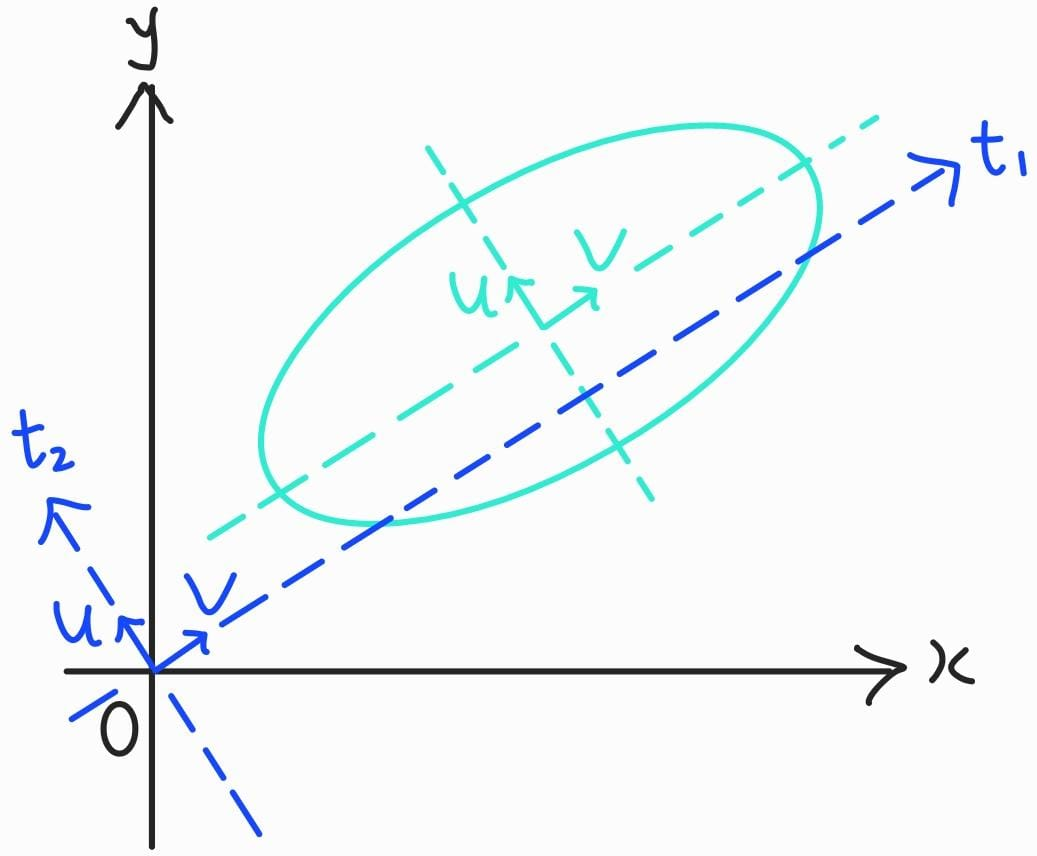
\includegraphics[width=0.5\textwidth]{../Diagrams/rotated-conics.jpg}
    \caption{\ref{Me} Rotated and translated conic.}
    \label{fig:rotated-conic}
\end{figure}
\begin{note}
    Without orthonormality, i.e. an isometric change of coordinates, even if we were successful in reducing our conic to the form \(a(x')^2+b(y')^2=f\), it may not prove to be a useful form. Consider the ellipse \(2x^2+2xy+y^2=1\). Clearly, \(x^2+(x+y)^2=1\). But, this gives a circle in \((x,x+y)\) coordinates; we can't deduce much about our initial conic. So, little meaning is found in such a factorisation. 
\end{note}
% Let \(\mathbf{x}\) and \(\mathbf{y}\) be the eigenvectors of \(\mathbf{M}\) corresponding to \(\lambda\) and \(\mu\). Since \(\mathbf{M}\) is symmetric, i.e. \(\mathbf{M}^T=\mathbf{M}\),
% \[\mathbf{x}\cdot\mu\mathbf{y}=(\mathbf{M}\mathbf{y})^{T}\mathbf{x}=(\mathbf{y}^T \mathbf{M}^T)\mathbf{x}=\mathbf{y}^T (\mathbf{M} \mathbf{x})=\mu \mathbf{x}\cdot \mathbf{y}.\]
% As such, \((\lambda-\mu)\mathbf{x}\cdot \mathbf{y}=0\). Hence, \(\mathbf{x}\cdot \mathbf{y}=0\).
% Consider the equation \(x^2+y=0\) and the matrix
% \(\mathbf{M}=\begin{pmatrix}
%     1 & 0\\
%     1 & 1
% \end{pmatrix}\). Then, \(x'=x\) and \(y'=x+y\). However, even though \(1^2-1=0\), we have \(1^2+(1-1)=1\neq 0\).
\chapter{Numerical Methods}
\begin{stbox}{General Information}
    \begin{itemize}
        \item The parity of the degree of a real polynomial is the same as that of its number of real roots.
        \item Let the real polynomial \(p\) given by \(p(x)=a_{2n}x^{2n}+a_{2n-1}x^{2n-1}+\dots+a_0\) have coefficients \(a_n>0\) and \(a_0<0\). Then, it has at least one positive and one negative root.
        \item To show that there a continuous function \(f\) attains a root in an interval \([a,b]\), we find two values \(x<y\) in the interval (e.g. \(a<b\)) such that \(f(a)f(b)<0\). i.e. show that \(f\) changes sign in \([a,b]\). Then, \emph{by continuity}, a root of \(f\) must lie in \([a,b]\).
        \item To further show that the root is \emph{unique} in \([a,b]\), it suffices to prove that \(f\) is \emph{strictly} monotone on \([a,b]\).
        \item Suppose we have some function \(f \colon \mathbb{R}\to \mathbb{R}\) with a root \(\alpha\), whose value we want to approximate. There are three ways to obtain this approximation.
        \begin{enumerate}
            \item Linear interpolation on an interval \([a,b]\) containing \(\alpha\). Our approximation is
            \[\frac{a \lvert f(b) \rvert+b \lvert f(a) \rvert}{\lvert f(a) \rvert+\lvert f(b) \rvert}.\]
            \begin{itemize}
                \item The sequence \(\{x_n\}\) of approximations \emph{always} converges to \(\alpha\).
                \item The smaller \(\lvert f''(x) \rvert\) is (i.e. the slower the gradient \(f'(x)\) changes) near \(\alpha\), the faster the rate of convergence.
                \item Error:
                \begin{table}[H]
                    \centering
                    \begin{tabular}{|Sc|Sc|Sc|}
                        \hline
                        Concave/Gradient & Positive & Negative\\
                        \hline
                        Upwards \(\bigcup\) & \textcolor{blue}{underestimation} & \textcolor{red}{overestimation}\\
                        \hline
                        Downwards \(\bigcap\) & \textcolor{red}{overestimation} & \textcolor{blue}{underestimation}\\
                        \hline
                    \end{tabular}
                    \caption{Approximation errors when using linear interpolation.}
                    \label{table:linear-interpolaion}
                \end{table}
                \item See Figure \ref{fig:linear-interpolation} for an illustration.
                \footnotetext{Screw trying to make nice diagonal cells. Pain. Suffering.}
            \end{itemize}
        \end{enumerate}
    \end{itemize}
\end{stbox}
\begin{note}
    At every iteration of linear interpolation, we must ensure that \(\alpha\in [a,x_n]\). Otherwise \(x_n\) may not approximate \(\alpha\). If \(\alpha\notin [a,x_n]\), simply consider \(\alpha\in [x_n,b]\) (or any other suitable interval) instead.
\end{note}
\begin{note}
    It is important to show which interval we are interpolating on, not just the iteratively obtained values. We can present our working using the table below.
    \begin{table}[H]
        \centering
        \begin{tabular}{|Sc|Sc|Sc|Sc|Sc|}
            \hline
            \(a\) & \(f(a)\) & \(b\) & \(f(b)\) & \(\dfrac{a \lvert f(b) \rvert+b \lvert f(a) \rvert}{\lvert f(a) \rvert+\lvert f(b) \rvert}\)\\
            \hline
            \(a\) & \(f(a)>0\) & \(b\) & \(f(b)<0\) & \(x_1\)\\
            \hline
            \(x_1\) & \(f(x_1)>0\) & \(b\) & \(f(b)<0\) & \(x_2\)\\
            \hline
            \(x_1\) & \(f(x_1)>0\) & \(x_2\) & \(f(x_2)<0\) & \(x_3\)\\
            \hline
            \(\vdots\) & \(\vdots\) & \(\vdots\) & \(\vdots\) & \(\vdots\)\\
            \hline
        \end{tabular}
        \caption{Required working for linear interpolation.}
        \label{table:linear-interpolation-presentation}
    \end{table}
\end{note}
\begin{stbox}{}
    \begin{itemize}
        \item[]
        \begin{enumerate}
            \item[2.] Fixed-point Iteration. First select a function \(F \colon \mathbb{R}\to \mathbb{R}\), such that \(F(\alpha)=\alpha\), and choose some initial approximation \(x_0\) to \(\alpha\). Then, we recursively define \(x_{n+1} \coloneq F(x_n)\). We want \(x_n\to \alpha\).
            \begin{itemize}
                \item Convergence behavior
                \begin{table}[H]
                    \centering
                    \begin{tabular}{|Sc|Sc|Sc|Sc|}
                        \hline
                        Behvaior of \(\lvert F'(x) \rvert\) & Converges? & Rate of convergence\\
                        \hline
                        \(\lvert F'(x) \rvert<1\) and is small near \(\alpha\) & \textcolor{green!70!black}{\checkmark} & \textcolor{green!70!black}{fast}\\
                        \hline
                        \(\lvert F'(x) \rvert<1\) but is close to 1 near \(\alpha\) & \textcolor{green!70!black}{\checkmark} & \textcolor{blue}{slow}\\
                        \hline
                        \(\lvert F'(x) \rvert\geq 1\) near \(\alpha\) & \textcolor{red}{\(\times\)} & -\\
                        \hline
                    \end{tabular}
                    \caption{Convergence behavior of fixed-point iterations.}
                    \label{table:fixed-point-iteration}
                \end{table}
                \item See Figure \ref{fig:fixed-point-iteration} for an illustration.
            \end{itemize}
        \end{enumerate}
    \end{itemize}
\end{stbox}
\begin{note}
    We must write out \emph{all} iterations, not just the final two. The working below is sufficient.

    \rule{20cm-137.0549pt}{0.05mm}

    \vspace{0.5\baselineskip} Let \(x_0=\rule{0.5cm}{0.05mm}\) and \(x_{n+1}=F(x_n)\), \(x\geq 0\).
    \begin{align*}
        x_1&=\rule{0.5cm}{0.05mm}\\
        x_2&=\rule{0.5cm}{0.05mm}\\
        &\vdotswithin{=}\\
        x_{m-1}&=\rule{0.5cm}{0.05mm}\\
        x_m&=\rule{0.5cm}{0.05mm}
    \end{align*}
    Therefore, \(\alpha=x_m\) (\(k\) d.p.), since \(f(x_m-0.0\cdots05)f(x_m+0.0\cdots05)=\rule{0.5cm}{0.01mm}<0\).
\end{note}
\begin{stbox}{}
    \begin{itemize}
        \item[]
        \begin{enumerate}
            \item[3.] The Newton-Raphson Method. Let \(\alpha\) be a root of the function \(f\colon \mathbb{R}\to \mathbb{R}\). The Newton-Raphson formula is
            \[x_{n+1}\coloneq x_n-\frac{f(x_n)}{f'(x_n)}.\]
            \begin{itemize}
                \item The Newton-Raphson method fails in the following cases.
                \begin{enumerate}
                    \item The gradient at \(x_0\) is too gentle.
                    \item The gradient changes too rapidly.
                    \item The initial approximation \(x_0\) is too far from the root \(\alpha\).
                    \item There is a turning point between the initial approximation \(x_0\) and the root \(\alpha\).
                    \item There is a point of inflection --- where the concavity changes/the sign of \(f''(x)\) changes.
                \end{enumerate}
                \item Error: 
                \begin{table}[H]
                    \centering
                    \begin{tabular}{|Sc|Sc|Sc|}
                        \hline
                        Concave/Gradient & Positive & Negative\\
                        \hline
                        Upwards \(\bigcup\) & \textcolor{red}{overestimation} & \textcolor{blue}{underestimation}\\
                        \hline
                        Downwards \(\bigcap\) & \textcolor{blue}{underestimation} & \textcolor{red}{overestimation}\\
                        \hline
                    \end{tabular}
                    \caption{Approximation errors when using the Newton-Raphson method.}
                    \label{table:newton-raphson}
                \end{table}
                \item See Figure \ref{fig:newton's-method} for an illustration.
            \end{itemize}
        \end{enumerate}
    \end{itemize}
\end{stbox}
\begin{note}
    We must write out \emph{all} iterations, not just the final two. One way to present our working is as follows.

    \rule{20cm-137.0549pt}{0.05mm}

    \vspace{0.5\baselineskip} Let \(x_0=\rule{0.5cm}{0.05mm}\) and \(x_{n+1}=x_n-\frac{f(x_n)}{f'(x_n)}=\rule{0.5cm}{0.05mm}\)\,, \(x\geq 0\).
    \begin{align*}
        x_1&=\rule{0.5cm}{0.05mm}\\
        x_2&=\rule{0.5cm}{0.05mm}\\
        &\vdotswithin{=}\\
        x_{m-1}&=\rule{0.5cm}{0.05mm}\\
        x_m&=\rule{0.5cm}{0.05mm}
    \end{align*}
    Therefore, \(\alpha=x_m\) (\(k\) d.p.), since \(f(x_m-0.0\cdots05)f(x_m+0.0\cdots05)=\rule{0.5cm}{0.01mm}<0\).
\end{note}
\begin{note}
    Explain whether \(x_0=\rule{0.5cm}{0.05mm}\) is a suitable starting value for using the Newton-Raphson method to find an approximation to \(\alpha\).
    
    \rule{20cm-137.0549pt-25pt}{0.05mm}
    \begin{figure}[H]
        \centering
        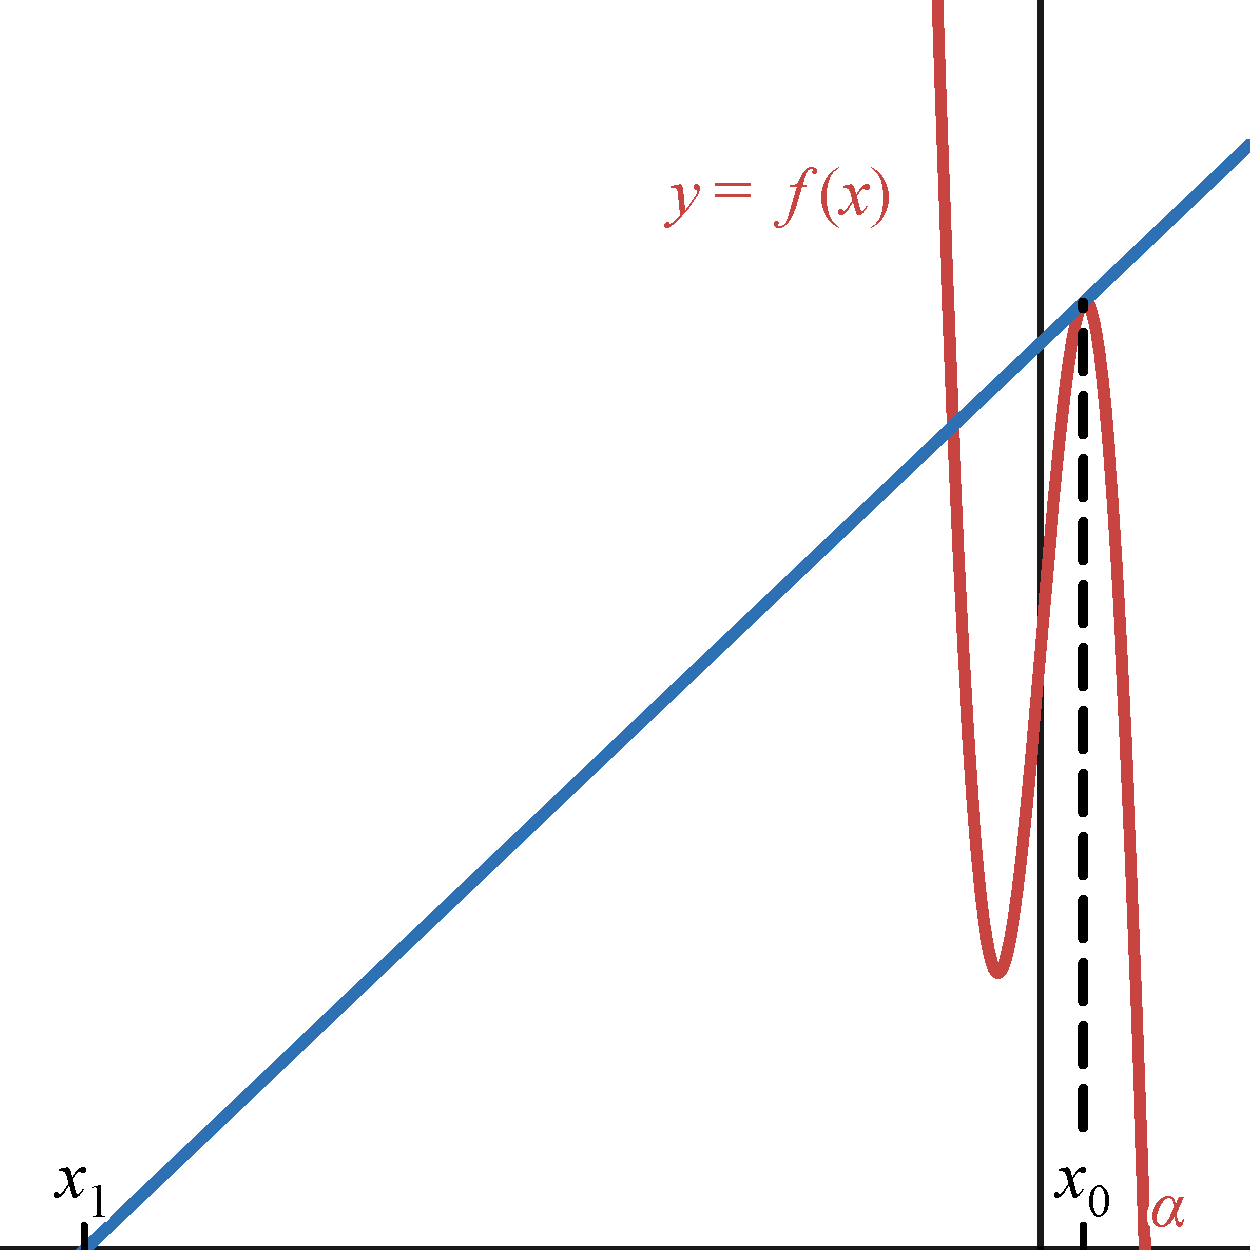
\includegraphics[width=0.5\textwidth]{../Diagrams/newton's-method-prelim.pdf}
        \caption{\ref{Me} \href{https://www.desmos.com/calculator/mq2elll5k3}{(Desmos)}}
        \label{fig:newton's-method-prelims}
    \end{figure}
    \begin{enumerate}
        \item Since \(x_0=\rule{0.5cm}{0.05mm}\) is very close to the stationary point, the tangent to the curve \(y=f(x)\) has a very gentle gradient. Thus, it cuts the \(x\)-axis far away from the initial approximation. 
        \item Furthermore, as \(x_0=\rule{0.5cm}{0.05mm}\) is to the left/right of the minimum/maximum point \(x=\rule{0.5cm}{0.05mm}\), the values of the gradient \(f'(x_n)\) will be negative/positive for all \(n\geq 0\). Hence, \(x_n\) converges to the root \(\beta\) instead \(\alpha\). 
    \end{enumerate}
    (The second point may be omitted if it is irrelevant.)
\end{note}
\begin{note}
    Suppose a question asks for the approximation of a root to \(k\) significant figures/\(k\) decimal places. Then: 
    \begin{enumerate}
        \item We leave our iterative approximations \(x_n\) to at least \(k+2\) significant figures/\(k+2\) decimal places.
        \item We continue the iterative process till two consecutive ones agree up to \(k\) significant figures/\(k\) decimal places.
    \end{enumerate}
\end{note}
\begin{note}
    Perform \rule{1.5cm}{0.01mm} (e.g. linear interpolation) to obtain an approximation for \(\alpha\), correct to two decimal places. Justify whether this approximation is sufficiently accurate.

    \rule{20cm-137.0549pt}{0.05mm}
    
    \vspace{0.5\baselineskip} Suppose our approximation is some \(a=1.00\), then we note the sign of \(f\) at \(a\pm 0.\highlight[yellow]{00}5\). (For an arbitrary number of s.f. or d.p., simply adjust the value \(0.\highlight[yellow]{00}5\) accordingly. E.g. for 3 d.p. we instead use \(0.\highlight[yellow]{000}5\)). Our working should look similar to the following:
    \begin{center}
        \parbox{0.9\textwidth}{
            Since \(f(0.995)=\rule{0.5cm}{0.01mm}<0\) and \(f(1.005)=\rule{0.5cm}{0.01mm}>0\), we conclude that \(1.00\) is a sufficiently accurate approximation, at 2 d.p..
        }
    \end{center}
\end{note}
\begin{note}
    The \emph{error obtained} when using an approximation should be the \emph{absolute} difference of the true value and the approximation. 
\end{note}
\begin{note}
    Use the results of part (i) and the differential equation \(dy/dx=\sin(xy)\) to estimate the \(x\)-coordinate \(x_P\) of \(P\). 

    \rule{20cm-137.0549pt}{0.05mm}

    \vspace{0.5\baselineskip} The maximum point occurs when \(dy/dx=\sin(xy)=0\), i.e. \(xy=k\pi\) where \(k\in \mathbb{Z}\). From (i), \(\frac{dy}{dx}\big|_{x=5/3}\approx 0.643>0\) so \(y_P>y(5/3)\approx 2.0468\). Hence, \(x_P\approx \pi/2.04679402=1.53\) (3.s.f).
\end{note}
\begin{GCSkills}{}
    Linear interpolation: finding an approximation to a root in \([a,b]\) up to \(n\) decimal places.
    \begin{enumerate}
        \item \(Y_1=f(x)\),
        \item \(a \to A\) and \(b \to B\),
        \item \(\dfrac{B \lvert Y_1(A) \rvert+A \lvert Y_1(B) \rvert}{\lvert Y_1(A) \rvert+\lvert Y_1(B) \rvert}\),
        \item \(\text{Ans}\to A \text{ or } B\) (choose the one that has the opposite sign to Ans),
        \item Repeat steps 4 to 5,
        \item Terminate this process when the approximations are consistent up to \(n\) decimal places.
    \end{enumerate}
    \end{GCSkills}
    You can freely enter any function and shift the initial values in the Desmos graphs below!
    \newpage
    \begin{figure}[H]
        \centering
        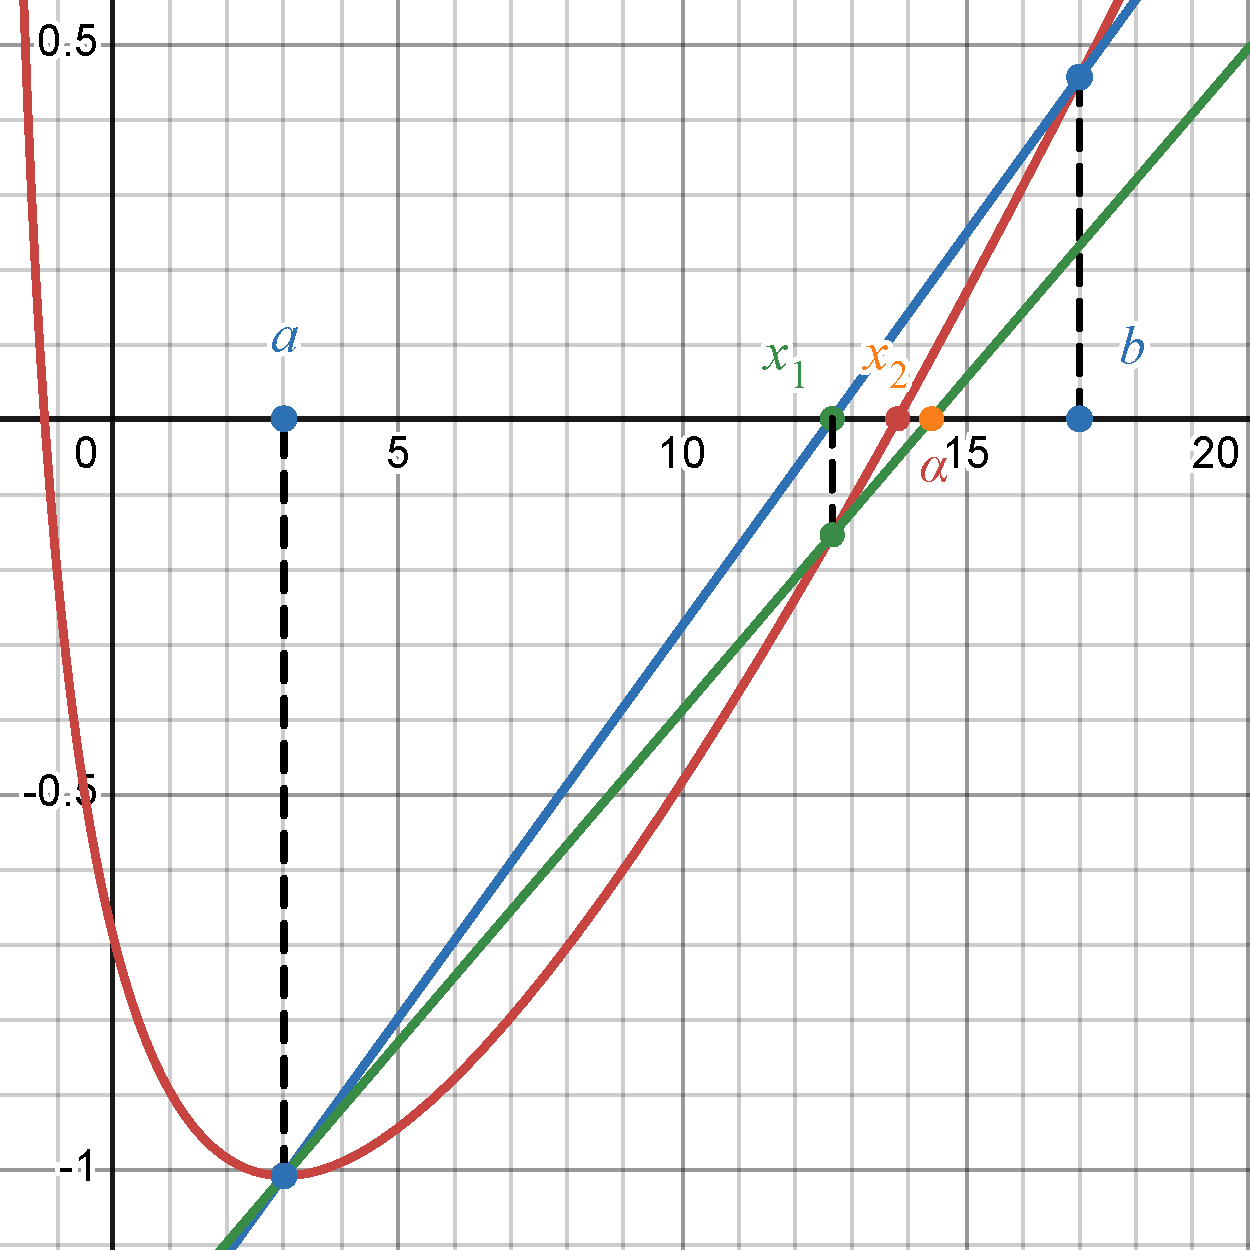
\includegraphics[width=0.69\textwidth]{../Diagrams/linear-interpolation.pdf}
        \caption{\ref{Me} An illustration of linear interpolation \href{https://www.desmos.com/calculator/yz71wfvkrl}{(Desmos)}.}
        \label{fig:linear-interpolation}
        % The second and third lines are wrong! 
    \end{figure}
    \begin{figure}[H]
        \centering
        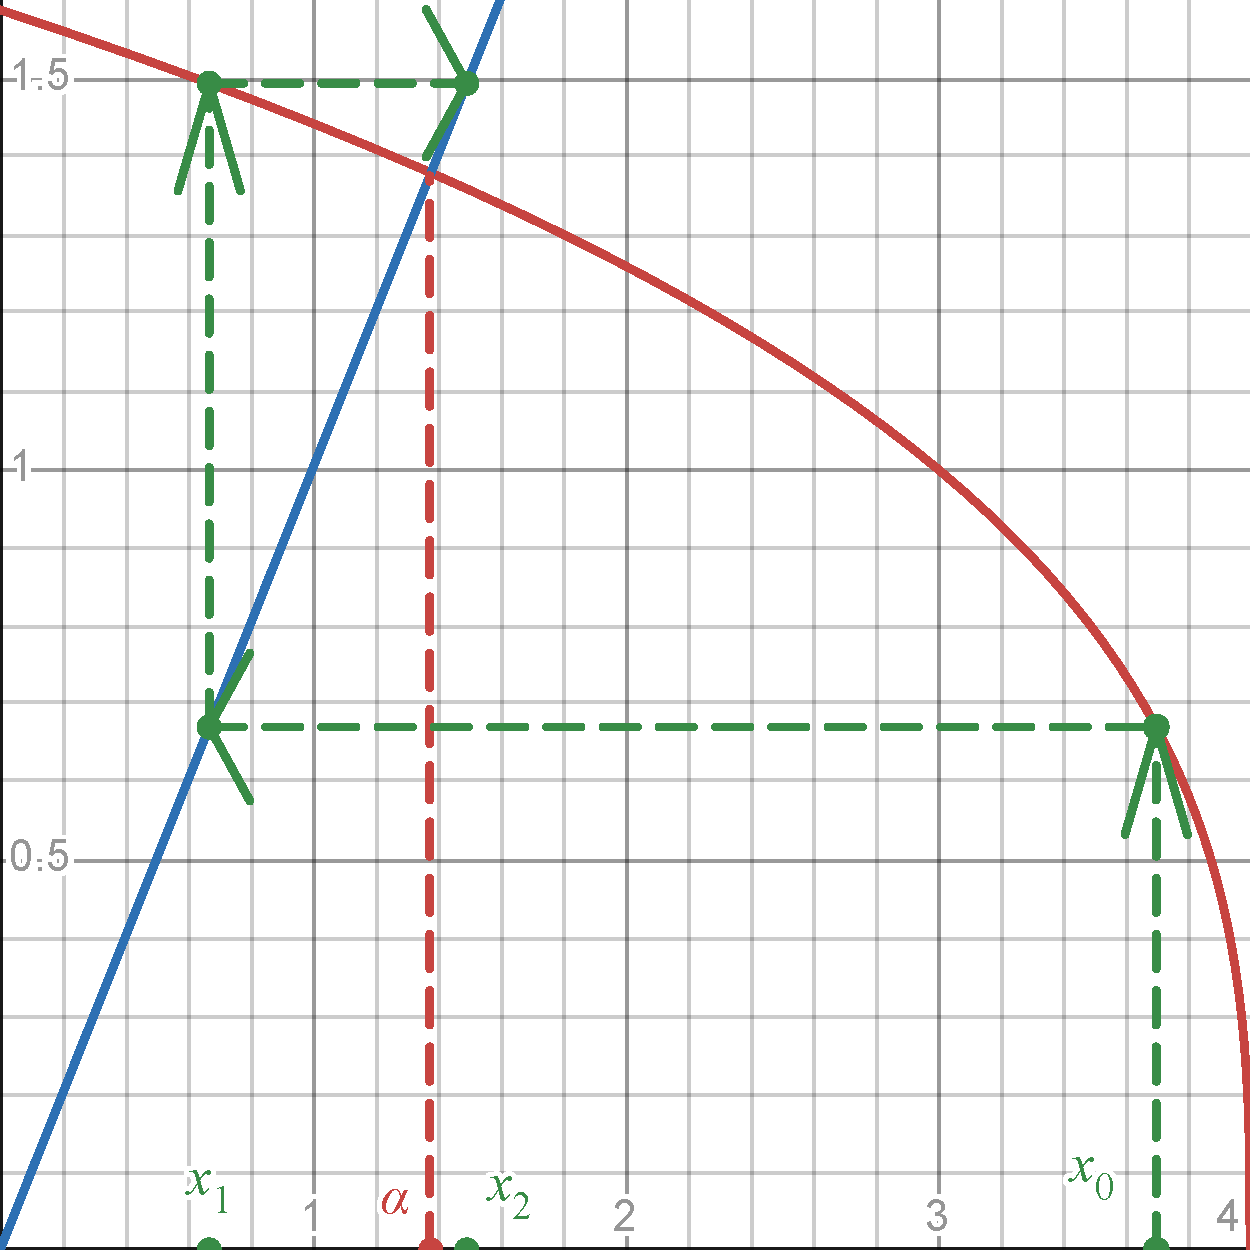
\includegraphics[width=0.69\textwidth]{../Diagrams/fixed-point-iteration/fixed-point-iteration-desmos.pdf}
        \caption{\ref{Me} An illustration of fixed-point iteration \href{https://www.desmos.com/calculator/t9mnqtmhxw}{(Desmos)}.}
        \label{fig:fixed-point-iteration}
    \end{figure}
    % \begin{figure}[H]
    %     \centering
    %     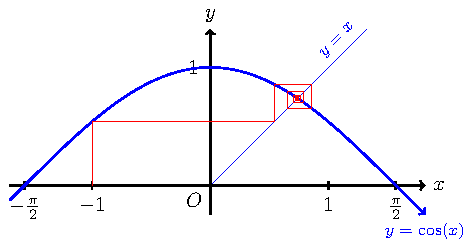
\includegraphics[width=\textwidth]{../Diagrams/fixed-point-iteration/fixed-point-iteration.pdf}
    %     \caption{An illustration of fixed-point iteration.}
    %     \label{fig:fixed-point-iteration}
    % \end{figure}
    \begin{figure}[H]
        \centering
        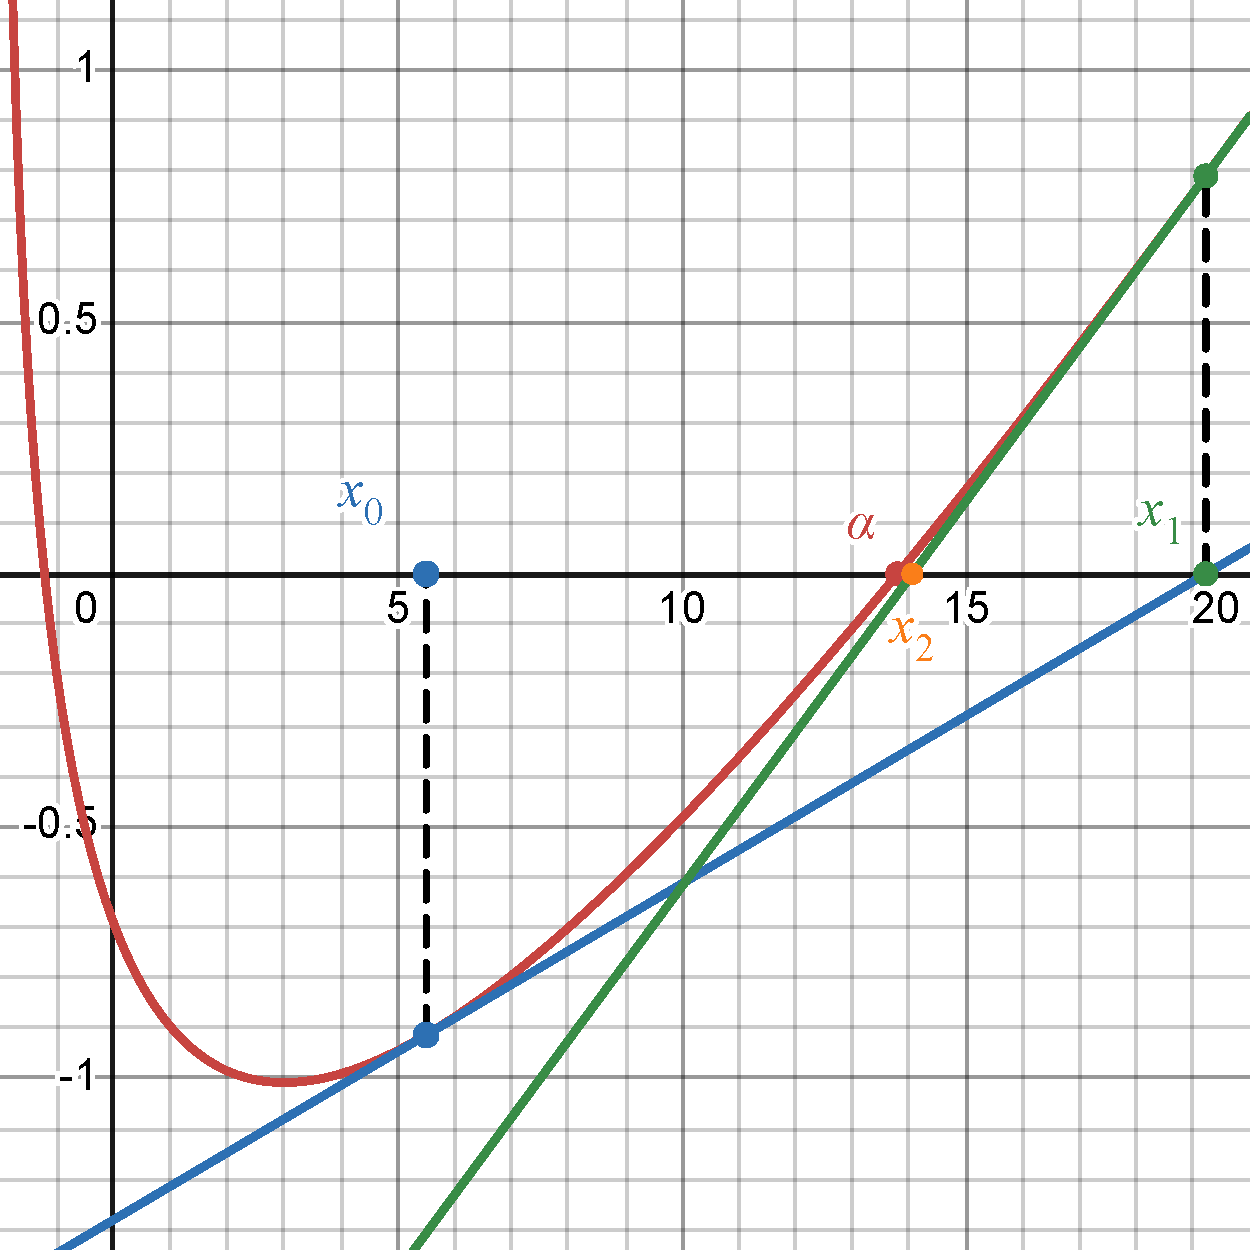
\includegraphics[width=0.69\textwidth]{../Diagrams/newton's-method.pdf}
        \caption{\ref{Me} An illustration of Newton's Method \href{https://www.desmos.com/calculator/izkg4ynlfp}{(Desmos)}.}
        \label{fig:newton's-method}
    \end{figure}
\part{FMB}
\chapter{Graphing Techniques}
\section{Graphing `Familiar' Functions and Asymptotic bois}

\begin{definition*}{}{}
  \begin{enumerate}
    \item \textbf{Lines of Symmetry}: A \emph{line of symmetry} of a function is a line, such that the function is a reflection of itself about that line.
    \item \textbf{Horizontal Asymptotes}: A (horizontal) line \(g(x)=c\) is the \emph{horizontal asymptote} of the curve \(f(x)\) iff \(\lim_{x \to \infty}{f(x)}=c\) (or with \(-\infty\) instead of \(\infty\)).\footnote{Otherwise notated by \(f(x) \to c\) as \(x \to \infty\).}
    \item \textbf{Vertical Asymptotes}: A (vertical) line \(x=c\) is a \emph{vertical asymptote} of the curve \(f(x)\) iff \(\lim_{x \to c}{f(x)}=\operatorname{\infty} \text{ or } -\infty\).
    \item \textbf{Oblique Asymptotes}: A line \(g(x)=mx+c\) --- where \(m \neq 0\) --- is an \emph{oblique asymptote} of the curve \(f(x)\) iff \(\lim_{x \to \infty}[f(x)-g(x)]=0\) (or with \(-\infty\) instead of \(\infty\)).
\end{enumerate}
\end{definition*}
\begin{stbox}{Curve Sketching of Rational Functions}
  \begin{enumerate}
    \item[\textbf{S}] Stationary points
    \item[\textbf{I}] Intersection with axes
    \item[\textbf{A}] Asymptotes   
  \end{enumerate}
  \begin{enumerate}[label=\roman*]
    \item Know how to sketch the graphs of \(y=\dfrac{ax+b}{cx+d}\) and \(y=\dfrac{ax^2+bx+c}{dx+e}\).
    \item Rectangular Hyperbolas \(\left(\text{of the form \(y=\dfrac{ax+b}{cx+d}\)}\right)\):
    \begin{itemize}
      \item \emph{Two} asymptotes, namely \(x=-\dfrac{d}{c}\) and \(y=\dfrac{a}{c}\).
      \item \emph{Two} lines of symmetry with gradients \(\pm 1\) \emph{and} pass through the intersection point of the aforementioned two asymptotes.
    \end{itemize}
    \item \emph{If} \(n=\operatorname{deg}P=\operatorname{deg}Q\), then
    \begin{itemize}
      \item \(y=R(x)\) is the \emph{horizontal} asymptote of \(\dfrac{P(x)}{Q(x)}=R(x)+\dfrac{S(x)}{Q(x)}\).
      \item Equivalently, \(y=\dfrac{\operatorname{coeff}_P(x^n)}{\operatorname{coeff}_Q(x^n)}\) is a \emph{horizontal} asymptote.\footnote{E.g.: \(y=\dfrac{1}{15}\) is a horizontal asymptote of \(y=\dfrac{\text{\hly{\(1\)}}x^2+2x-3}{(\text{\hly{\(5\)}}x+1)(\text{\hly{\(3\)}}x+2)}\).}
    \end{itemize}
    \item If \(\operatorname{deg}P=\operatorname{deg}Q+1\), then \(R(x)\) is an \emph{oblique} asymptote of \(\dfrac{P(x)}{Q(x)}=R(x)+\dfrac{S(x)}{Q(x)}\).
    \item Write down asymptotes and lines of symmetry.\footnote{E.g.: \begin{itemize}
      \item[] Asymptotes: \(x=4\), \(y=20\).
      \item[] Lines of Symmetry: \(y=x+16\), \(y=-x+24\).
    \end{itemize} } If none are present indicate with ``No lines of symmetry.''
  \end{enumerate}
\end{stbox}
\begin{IN}
  \begin{itemize}
    \item The discriminant can be very useful.
    \item Be aware of how to use the G.C. Transfrm app.
    It allows you to vary the value of some parameter \(A\) for a function \(f(Ax)\). Use this to graphically find the values of \(k\) that satisfy some condition(s).
  \end{itemize}
\end{IN}

\section{Conics}
``Tikz is pain, PGFPlots is suffering'' --- Wise Man.
\begin{center}
  \small
  \begin{tabular}{|c|c|c|}
    \hline
    & Ellipses & Hyperbolas\\
    \hline
    Standard Forms & \(\dfrac{(x-h)^2}{a^2}+\dfrac{(y-k)^2}{b^2}=1\) & 
    \begin{tabular}{@{}c@{}} 
     \\
    \(\dfrac{(x-h)^2}{a^2}-\dfrac{(y-k)^2}{b^2}=1\)\\
    \(\dfrac{(y-k)^2}{b^2}-\dfrac{(x-h)^2}{a^2}=1\)\\
    \\
    \end{tabular}\\
    \hline
    General Equation & 
    \begin{tabular}{@{}c@{}} 
      \(ax^2+by^2+cx^2+dx+e=0\),\\
      \footnotesize where \(\operatorname{sgn}(a)=\operatorname{sgn}b\). \normalsize
     \end{tabular}
     &
     \begin{tabular}{@{}c@{}} 
      \(ax^2+by^2+cx^2+dex+e=0\),\\
      \footnotesize where \(\operatorname{sgn}(a) \neq \operatorname{sgn}b\). \normalsize
     \end{tabular}\\
     \hline
     Center & \multicolumn{2}{c|}{\((h,k)\)}\\
    \hline
    \begin{tabular}{@{}c@{}} 
      Vertical `Radius'\\
      \footnotesize (variables here from \emph{standard form}!) \normalsize
    \end{tabular}
      & \multicolumn{2}{c|}{\(b\)}\\
      \hline
    \begin{tabular}{@{}c@{}} 
        Horizontal `Radius'\\
        \footnotesize (variables here from \emph{standard form}!) \normalsize
    \end{tabular}
    & \multicolumn{2}{c|}{\(a\)}\\
    \hline
    \begin{tabular}{@{}c@{}} 
      Vertical  Vertices\\
      \footnotesize (variables here from \emph{standard form}!) \normalsize
    \end{tabular}
    & \multicolumn{2}{c|}{\((h, k \pm b)\)}\\
    \hline
    \begin{tabular}{@{}c@{}} 
      Horizontal Vertices\\
      \footnotesize (variables here from \emph{standard form}!) \normalsize
    \end{tabular}
    & \multicolumn{2}{c|}{\((h \pm a,k)\)}\\
    \hline
    Shape & 
    \begin{tikzpicture}[scale=0.5]
      
      \begin{axis}[axis lines=middle,axis line style =-{Classical TikZ Rightarrow[length=5pt 3 0]},every axis x label/.style = {%
        at = {(xticklabel cs:1.05)},
        anchor = north},
      every axis y label/.style = {%
        at = {(yticklabel cs:1.05)},
        anchor=east},
        xtick=\empty, ytick=\empty,clip=false,xmin=0,xmax=11,xlabel=\Large\(x\),ylabel=\Large\(y\),ymin=0,ymax=6
        ]
        
      \draw[blue] (5,3) ellipse (5 and 2);
    
      % label center
      \node at (5,3) [below right] {\Large \((h,k)\)};

      \node at (5,3) {\Large \color{red}{\(\times\)}};
    
      % draw h-line
      \draw[->,arrows = -{Classical TikZ Rightarrow[length=5pt 3 0]}] (5,3) -- (0,3) node[midway, above] {\Large \(a\)};
    
      % draw another h-line
      \draw[->,arrows = -{Classical TikZ Rightarrow[length=5pt 3 0]}] (5,3) -- (10,3);
    
      % draw k-line
      \draw[->,arrows = -{Classical TikZ Rightarrow[length=5pt 3 0]}] (5,3) -- (5,5) node[midway, right] {\Large \(b\)};
    
      % draw another k-line
      \draw[->,arrows = -{Classical TikZ Rightarrow[length=5pt 3 0]}] (5,3) -- (5,1);

      \addplot+[
  mark=x,
  only marks,
  mark size=6pt,
  mark options={line width=1.5pt,red}
] 
  coordinates
  {(5,3)};
  
      \end{axis}
      % draw ellipse
      \addvmargin{3mm}
    \end{tikzpicture} & 
    \begin{tabular}{@{}c@{}} 
      \(\operatorname{coeff}(x^2)<0\)\\
      \begin{tikzpicture}[scale=0.5]
      
        \begin{axis}[axis lines=middle,axis line style =-{Classical TikZ Rightarrow[length=5pt 3 0]},every axis x label/.style = {%
          at = {(xticklabel cs:1.05)},
          anchor = north},
        every axis y label/.style = {%
          at = {(yticklabel cs:1.05)},
          anchor=east},
          xtick=\empty, ytick=\empty,clip=false,xmin=-1,xmax=11,xlabel=\Large\(x\),ylabel=\Large\(y\),ymin=-1,ymax=7
          ]
          
      \addplot [red,thick,domain=-2:2] ({sinh(x)+5}, {cosh(x)+3});
      \addplot [red,thick,domain=-2:2] ({-sinh(x)+5}, {-cosh(x)+3});
      \addplot[red,dashed,domain=1:9] {x-2};
      \addplot[red,dashed,domain=1:9] {-x+8};

        \node at (5,3) [below] {\Large \((h,k)\)};
  
        \node at (5,3) {\LARGE  \color{blue}{\(\times\)}};
      
        % draw h-line
        \draw[->,arrows = -{Classical TikZ Rightarrow[length=3pt 3 0]}] (5,4) -- (4,4) node[midway, above] {\Large \(a\)};
      
        % draw k-line
        \draw[->,arrows = -{Classical TikZ Rightarrow[length=3pt 3 0]}] (5,3) -- (5,4) node[midway, right] {\Large \(b\)};
        
        \addplot+[
  mark=x,
  only marks,
  mark size=6pt,
  mark options={line width=1.5pt}
] 
  coordinates
  {(5,3)};

        \end{axis}
        % draw ellipse
      \end{tikzpicture}\\
      \(\operatorname{coeff}(y^2)<0\)\\
      \begin{tikzpicture}[scale=0.5]
      
        \begin{axis}[axis lines=middle,axis line style =-{Classical TikZ Rightarrow[length=5pt 3 0]},every axis x label/.style = {%
          at = {(xticklabel cs:1.05)},
          anchor = north},
        every axis y label/.style = {%
          at = {(yticklabel cs:1.05)},
          anchor=east},
          xtick=\empty, ytick=\empty,clip=false,xmin=-1,xmax=11,xlabel=\Large\(x\),ylabel=\Large\(y\),ymin=-1,ymax=7
          ]
          
        \addplot [red,thick,domain=-2:2] ({cosh(x)+5}, {sinh(x)+3});
      \addplot [red,thick,domain=-2:2] ({-cosh(x)+5}, {sinh(x)+3});
      \addplot[red,dashed,domain=1:9] {x-2};
      \addplot[red,dashed,domain=1:9] {-x+8};

        \node at (5,3) [below=0.25cm] {\Large \((h,k)\)};
  
        \node at (5,3) {\LARGE  \color{blue}{\(\times\)}};
      
        % draw h-line
        \draw[->,arrows = -{Classical TikZ Rightarrow[length=3pt 3 0]}] (5,3) -- (4,3) node[midway, above] {\Large \(a\)};
      
        % draw k-line
        \draw[->,arrows = -{Classical TikZ Rightarrow[length=3pt 3 0]}] (4,3) -- (4,4) node[midway, left] {\Large \(b\)};

        \addplot+[
  mark=x,
  only marks,
  mark size=6pt,
  mark options={line width=1.5pt}
] 
  coordinates
  {(5,3)};

        \end{axis}
        % draw ellipse
      \end{tikzpicture}
    \end{tabular}\\
    \hline
    \begin{tabular}{@{}c@{}} 
      Asymptotes\\
      (No need to rmb!)
    \end{tabular}
    & - & \(y=k \pm \dfrac{b(x-h)}{a}\)\\
    \hline
    Lines of Symmetry & \multicolumn{2}{c|}{\(x=h\), \(y=k\)}\\
    \hline
  \end{tabular}
  \normalsize
\end{center}
\begin{stbox}{General Information}
  \begin{itemize}
    \item To find asymptote of hyperbolas, solve  
    \[\frac{(x-h)^2}{a^2}=\frac{(y-k)^2}{b^2}.\]
    \item When sketching any conic, label its vertices or radii, together with its center and asymptotes.
  \end{itemize}
\end{stbox}
\section{Parametric Equations}
\begin{IN}
  \begin{itemize}[label=\(\star\)]
    \item Check the qns for any \emph{restrictions} on the parameter! And modify that of the G.C.'s accordingly (Tmin \& Tmax).
    \item Vary the \(t\)-step or resolution (when using cartesian coordinates) when the graph is oddly jagged.
  \end{itemize}
\end{IN}
\section{Scaling, Translations, and Reflections}

\begin{center}
  \begin{tabular}{|Sc|Sc|Sc|}
    \hline
    \multicolumn{3}{|Sc|}{\large \color{blue}{Playing With \(x\)}}\\
    \hline
    Function & \(x\) is replaced with & (Horizontal) Transformation\\
    \hline 
    \(f(x+a)\) & \(x+a\) & 
    \begin{tabular}{@{}c@{}} 
      Translate \(a\) units in the positive (\(a \leq 0\))\\ 
      O/R negative \(x\)-direction (\(a \geq 0\)).
    \end{tabular}\\
    \hline 
    \(f(-x)\) & \(-x\) & Reflect about the \(y\)-axis\\
    \hline
    \(f(ax)\) & \(ax\) & Scale parallel to the \(x\)-axis by a scale factor of \(\dfrac{1}{a}\) if \(a \geq 0\).\\
    \hline
    \multicolumn{3}{|Sc|}{\large \color{red}{Playing With \(f(x)\)}}\\
    \hline
    \multicolumn{2}{|c|}{Function / Change to \(f(x)\)} & (Vertical) Transformation\\
    \hline
    \multicolumn{2}{|c|}{\(f(x)+a\)} & \begin{tabular}{@{}c@{}} 
      Translate \(a\) units in the positive (\(a \geq 0\))\\ 
      O/R negative \(y\)-direction (\(a \leq 0\)).
    \end{tabular}\\
    \hline
    \multicolumn{2}{|c|}{\(-f(x)\)} & Reflect about the \(x\)-axis.\\
    \hline
    \multicolumn{2}{|c|}{\(af(x)\)} & Scale parallel to the \(y\)-axis by scale factor \(a\).\\
    \hline
  \end{tabular}
\end{center}
\begin{IN}
\begin{center}
  \begin{tikzpicture}
    \node[ellipse, draw=blue, thick, minimum size=10mm,align=center] (x) at (1,0) {Transform \(x\)\\[2mm]
    Translation \ding{239} Scaling / Reflection};
    \node[ellipse, draw=red, thick, minimum size=10mm,align=center] (y) at (1,-3) {Transform \(y\)\\[2mm]
    Scaling / Reflection \ding{239} Translation};
    \draw [black, line width=0.75pt, arrows = {-Latex[open,scale=2]}] (x) to (y);
  \end{tikzpicture}
\end{center}
\end{IN}
\newpage
\section{\(\lvert f(x) \rvert\) and \(f( \lvert x \rvert)\)}
\begin{stbox}{General Information}
  \begin{itemize}
    \item For \(\lvert f(x) \rvert\), simply flip the part of the graph of \(f(x)\) that is below the \(x\)-axis, to above the \(x\)-axis.
    \item For \(f(\lvert x \rvert)\), its graph is symmetric about the \(x\)-axis
  \end{itemize}
\end{stbox}
\section{\(y=\frac{1}{f(x)}\)}
\begin{center}
  \begin{tabular}{|Sc|Sc|}
    \hline
    Behavior of \(f(x)\) & Behavior of \(1/f(x)\)\\
    \hline
    \(f(x)>0\) & \(\dfrac{1}{f(x)}>0\)\\
    \hline 
    \(f(x)<0\) & \(\dfrac{1}{f(x)}<0\)\\
    \hline
    Vertical Asymptote at \(x=c\) & \begin{tabular}{@{}c@{}} 
      \(\dfrac{1}{f(x)}\) \emph{tends} to 0\\
      \scriptsize \(^{*}\dfrac{1}{f(x)}\) is undefined at \(x=c\) \normalsize\\
    \end{tabular}\\
    \hline
    \multicolumn{2}{|Sc|}{\begin{tabular}{@{}c@{}} 
      \(\dfrac{df}{dx}=-\dfrac{d}{dx}\mathopen{}\left(\dfrac{1}{f(x)}\right)\)\\
      \scriptsize i.e. when \(f(x)\) increases, \(\dfrac{1}{f(x)}\) decreases. \normalsize\\
    \end{tabular}}\\
    \hline 
    \((a,b)\) is a \emph{minimum} pt & \(\left(a,\dfrac{1}{b}\right)\) is a \emph{maximum} pt\\
    \hline
    \((a,b)\) is a \emph{maximum} pt & \(\left(a,\dfrac{1}{b}\right)\) is a \emph{minimum} pt\\
    \hline
  \end{tabular}
\end{center}
\chapter{Polar Curves}
\begin{figure}[H]
  \centering
  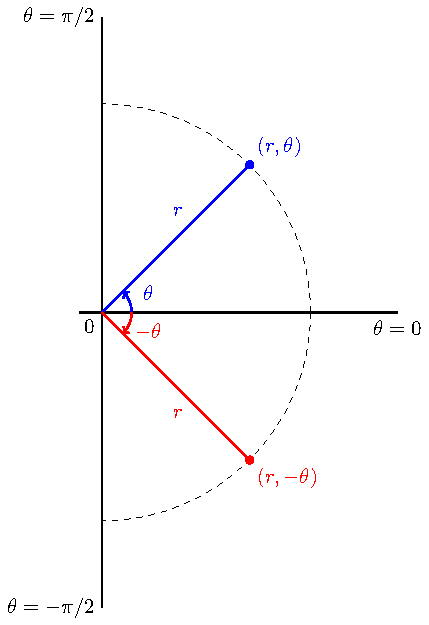
\includegraphics{../Diagrams/polar-form-illustration/polar.pdf}
  \caption{\ref{source:polar-coordinates} Polar coordinates.}
  \label{fig:polar-coordinates}
\end{figure}
\begin{definition*}{}{}
  \begin{enumerate}
    \item The \emph{pole} is the origin.
    \item The \emph{initial line/polar axis} is the \emph{half line} \(\theta=0\).
  \end{enumerate}
\end{definition*}
\begin{stbox}{General Information}{}
  \begin{itemize}[label=\(\circ\)]
    \item Coordinate Conversion
    \begin{center}
      \begin{tabular}{|Sc|Sc|}
        \hline
        \(\begin{aligned}
          r &= \sqrt{x^2+y^2}\\
          \theta &= \tan^{-1}\left(\dfrac{y}{x}\right)
        \end{aligned}\) &
        \(\begin{aligned}
          x &= r \cos(\theta)\\
          y &= r \sin(\theta)
        \end{aligned}\)\\
        \hline
      \end{tabular}
    \end{center}
    \item Standard Functions
    % Marking TABLE 
    %TABLE IS HERE
    %
    \begin{longtable}{|Sc|Sc|Sc|}
      \hline
    Polar Equation & Cartesian Equation\\
    \hline
\begin{tabular}{@{}Sc@{}}
  \begin{tikzpicture}[scale=0.4]
    %Axis
    \draw[thick] (-2.5ex,0) -- (7,0) node [below] {\(\theta=0\)};
    \draw[thick] (0,-2) 
    node [left] {} 
    -- (0,2) 
    node [left] {\(\theta=\dfrac{\pi}{2}\)};

    \node[anchor=north east] (Origin) at (0,0) {\(0\)};

    \draw[thick,blue] (3.5,-2) node [below] {\(r \cos(\theta)=a\)} -- (3.5,2);
  \end{tikzpicture}
\end{tabular} & \(x=a\)\\
\hline
\begin{tabular}{@{}Sc@{}}
  \begin{tikzpicture}[scale=0.4]
    %Axis
    \draw[thick] (-2.5ex,0) -- (7,0) node [below] {\(\theta=0\)};
    \draw[thick] (0,-2) 
    node [left] {} 
    -- (0,2) 
    node [left] {\(\theta=\dfrac{\pi}{2}\)};

    \node[anchor=north east] (Origin) at (0,0) {\(0\)};

    \draw[thick,blue] (-2em,1) -- (7,1) node [above] {\(r \sin(\theta)=a\)};
  \end{tikzpicture}
\end{tabular}& \(y=a\)\\
\hline
\begin{tabular}{@{}Sc@{}}
  \begin{tikzpicture}[scale=0.4]
    %Axis
    \draw[thick] (-2.5ex,0) -- (7,0) node [below] {\(\theta=0\)};
    \draw[thick] (0,-2) 
    node [left] {} 
    -- (0,2) 
    node [left] {\(\theta=\dfrac{\pi}{2}\)};

    \node[anchor=north east] (Origin) at (0,0) {\(0\)};

    \draw[thick,blue] (0,0) -- (7,2) node [above right] {\(\theta=\alpha\)};

    \coordinate (A) at (7,0);
    \coordinate (B) at (0,0);
    \coordinate (C) at (7,2);
    \pic[draw, -, blue, thick, "\small \(\alpha\) \normalsize", angle eccentricity=1.7] {angle = A--B--C};
  \end{tikzpicture}
\end{tabular}& \(y=x\tan(\alpha)\)\\
\hline
\begin{tabular}{@{}Sc@{}}
  \begin{tikzpicture}[scale=0.4]
    %Axis
    \draw[thick] (-3,0) -- (3,0) node [below] {\(\theta=0\)};
    \draw[thick] (0,-3) 
    node [left] {} 
    -- (0,3) 
    node [left] {\(\theta=\dfrac{\pi}{2}\)};

    \node[anchor=north east] (Origin) at (0,0) {\(0\)};
    \node[above right, blue] (Circle) at (0,2) {\(r=a\)};
    \draw[thick,blue] (0,0) circle [radius=2cm];
  \end{tikzpicture}
\end{tabular}& \(x^2+y^2=a^2\)\\
\hline
\begin{tabular}{@{}Sc@{}}
\begin{tikzpicture}[scale=0.4]
  %Axis
  \draw[thick] (-2em,0) -- (5,0) node [below] {\(\theta=0\)};
  \draw[thick] (0,-3) 
  node [left] {} 
  -- (0,3) 
  node [left] {\(\theta=\dfrac{\pi}{2}\)};

  \node[anchor=north east] (Origin) at (0,0) {\(0\)};
  \node[above, blue] (Circle) at (2.5,2) {\(r=a \cos(\theta)\)};
  \draw[thick,blue] (2,0) circle [radius=2cm];
\end{tikzpicture} 
\end{tabular}& \(\left(x-\dfrac{a}{2}\right)^2+y^2=\dfrac{a^2}{4}\)\\
\hline
\begin{tabular}{@{}Sc@{}}
\begin{tikzpicture}[scale=0.4]
  %Axis
  \draw[thick] (-3,0) -- (3,0) node [below] {\(\theta=0\)};
  \draw[thick] (0,-2em) 
  node [left] {} 
  -- (0,5) 
  node [left] {\(\theta=\dfrac{\pi}{2}\)};

  \node[anchor=north east] (Origin) at (0,0) {\(0\)};
  \node[above right, blue] (Circle) at (0,4) {\(r=a \sin(\theta)\)};
  \draw[thick,blue] (0,2) circle [radius=2cm];
\end{tikzpicture} 
\end{tabular}& \(x^2+\left(y-\dfrac{a}{2}\right)^2=\dfrac{a^2}{4}\)\\
\hline
    \end{longtable}
    \item Tangent lines at the pole are obtained by solving \(r=0\).
    \item \(r=f(\theta)\) is symmetrical about the polar (horizontal) axis iff \(f(\theta)=f(-\theta)\) for all \(\theta\).
    \item \(r=f(\theta)\) is symmetrical about the vertical line \(\theta=\pi/2\) iff \(f(\theta)=f(\pi-\theta)\) for all \(\theta\).
    \item Suppose \(r\) is a function of \(\cos(n\theta)\)\emph{only}. E.g. \(r=a\sqrt{(4+\sin^2(\theta))^2\cos(\theta)}\). Then, the lines of symmetry are \(n\theta=k\pi\), for \(k\in \mathbb{Z}\).
    \item Suppose \(r\) is a function of \(\sin(n\theta)\) \emph{only}. Then, the lines of symmetry are \(n\theta=k\pi/2\), for \(k\in \mathbb{Z}\).
    \item \(r=f(\theta)\) is symmetrical about the pole iff \((r,\theta)\) is a point on the curve whenever \((-r,\theta)\) is.
    \item The use of \hyperlink{R-formulas}{\(R\)-formulas} may be necessary.
    \item Area of a sector, 
    \[A=\dfrac{1}{2}\int_{\alpha}^{\beta}r^2\,\text{d}\theta,\] 
    where \(\alpha<\beta\).
    \item Arc length, 
    \[\ell=\int_{\theta_1}^{\theta_2} \sqrt{r^2+\left(\frac{dr}{d\theta}\right)^2}\,\text{d}\theta.\]
  \end{itemize}
\end{stbox}
\begin{IN}
  \begin{enumerate}
    \item Normally, \(r\geq 0\). But, in some questions, it can be negative.
    \item There is no need to fully expand/simplify our final answers. E.g. \((x^2+y^2)^2=3y(x^2+y^2)-4y^2\) suffices.
    \item The essentials of sketching polar curves:
    \begin{enumerate}
      \item Shape of curve
      \item Intersection(s) with (`axial') half lines
      \item Nothing else \emph{unless} the qns asks for it
    \end{enumerate}
    \begin{enumerate}[label=\(\qed\)]
      \item Be careful of the sharpness / smoothness of points! Points supposed to be sharp should be sufficiently so, and those supposed to be smooth should be sufficiently rounded / not look sharp.
      \item Check whether the polar axes are tangents at pole. Use this information to draw accurate graphs.
      \item Best to add a small dotted line to show tangentiality at intercepts.
      \item Careful about constants like \(a\) in \(r=a\sin(\theta)\) for axial intercepts.
      \item No need to state points at the pole unless they are `axial', i.e. \(\theta=0\), or \(\pi/2\), etc.
    \end{enumerate}
    \item When finding maximum / minimum \(y\) values \(\left(dy/dx=0\right)\), we need to check its nature (1st/2nd deriv test). However, this is unnecessary for max / min \(r\) values.
    \item When finding \(dy/dx\), try to keep it in polar form if possible instead of converting to cartesian form.
    \item As usual, be \emph{careful}, such as about which values need to be rejected.
    \item When reflecting/rotating, a diagram may be useful to find the angle/expression to replace \(\theta\) with. E.g.: \small
    \begin{enumerate}
      \item To reflect about \(r=\theta\) or \(y=x\), we map \((r,\theta) \to (r,\pi/2-\theta)\).
      \item A reflection about the half-line \(\theta=\pi/2\) is obtained by mapping \((r,\theta) \to (r,\pi-\theta)\).
    \end{enumerate} \normalsize
  \end{enumerate}
\end{IN}
\begin{GCSkills}{}
  \begin{enumerate}
    \item To display a nicely scaled polar curve, we use \texttt{Zoom fit}, followed by \texttt{Zoom square}
    \item Press alpha trace 1 to get \(r_1\). In fact, this works for the other modes available in the GC as well. 
    \item We can type 
    \[\left. \frac{d}{d\theta}r_1 \right\rvert_{\theta=\theta}\] 
    into formulas (e.g. for arc length) without having to manually differentiate it!
  \end{enumerate}
\end{GCSkills}
\chapter{Conic Sections}
\begin{definition}{}{}
  Eccentricity \(e\) is defined as 
  \[\frac{\text{distance of \(P\) from focus}}{\text{distance of \(P\) from directrix}}.\]
\end{definition}
\begin{stbox}{General Information}{}
  \begin{table}[H]
    \centering
    \begin{tabular}{ScScScScSc}
      \toprule
      Conic section & Circle & Ellipse & Parabola & Hyperbola\\
      \midrule
      Eccentricity \(e\) & \(0\) & \((0,1)\) & \(1\) & \((1,\infty)\)\\
      \bottomrule
    \end{tabular}
    \caption{Values of eccentricity \(e\) and the associated conic sections.}
    \label{table:eccentricity-associated-conics}
  \end{table}
  \resizebox{\columnwidth}{!}{\begin{tabular}{|Sc|Sc|Sc|Sc|Sc|Sc|Sc|}
    \hline 
    Conic & \multicolumn{2}{Sc|}{Parabolas} & \multicolumn{2}{Sc|}{Ellipses} & \multicolumn{2}{Sc|}{Hyperbolas}\\
    \hline
    Cartesian & \(x^2=4py\) & \(y^2=4px\) & 
    \(\begin{aligned}
      \frac{x^2}{a^2}+\frac{y^2}{b^2}=1\text{, }a>b
    \end{aligned}\) & 
    \(\begin{aligned}
    \frac{x^2}{a^2}+\frac{y^2}{b^2}=1\text{, }b>a
    \end{aligned}\) &
    \(\begin{aligned}
    \frac{x^2}{a^2}-\frac{y^2}{b^2}=1
    \end{aligned}\) & 
    \(\begin{aligned}
    \frac{y^2}{b^2}-\frac{x^2}{a^2}=1
    \end{aligned}\)\\
    \hline
    Parametric & 
    {\(\!\begin{aligned} 
      x&=t\\
      y&=t^2/4p
     \end{aligned}\)} &
     {\(\!\begin{aligned}
      x&=t^2/4p\\
      y&=t
    \end{aligned}\)} & 
    \multicolumn{2}{Sc|}{\(x=a\cos(\theta)\), \(y=b\sin(\theta)\)} &
    {\(\!\begin{aligned} 
      x&=a\sec(\theta)\\
      y&=b\tan(\theta)
     \end{aligned}\)} &
     {\(\!\begin{aligned}
      x&=a\tan(\theta)\\
      y&=b\sec(\theta)
    \end{aligned}\)}\\
    \hline
    Foci & \((0,p)\) & \((p,0)\) & \((\pm c,0)\) & \((0,\pm c)\) & \((\pm c,0)\) & \((0,\pm c)\)\\
    \hline
    \(a,b,c\) & \multicolumn{2}{Sc|}{N.A.} & \(c^2=a^2-b^2\) & \(c^2=b^2-a^2\) & \multicolumn{2}{Sc|}{\(c^2=a^2+b^2\)}\\
    \hline
    Directrices & \(y=-p\) & \(x=-p\) & 
    \(\begin{aligned}
      x=\pm\frac{a}{e}=\pm\frac{a^2}{c}
    \end{aligned}\) & 
    \(\begin{aligned}
    y=\pm\frac{b}{e}=\pm\frac{b^2}{c}
    \end{aligned}\) & 
    \(\begin{aligned}
    x=\pm\frac{a}{e}=\pm\frac{a^2}{c}\end{aligned}\) & 
    \(\begin{aligned}
    y=\pm\frac{b}{e}=\pm\frac{b^2}{c}
    \end{aligned}\)\\
    \hline
    \multirow{2}{*}[-1cm]{e} & \multicolumn{2}{Sc|}{\(e=1\)} & \multicolumn{2}{Sc|}{\(0<e<1\)} & \multicolumn{2}{Sc|}{\(e>1\)}\\
    \cline{2-7}
    & \multicolumn{2}{Sc|}{N.A.} & 
    \(\begin{aligned}
      e&=\frac{c}{a}\\
      &=\frac{\sqrt{a^2-b^2}}{a}\\
      &=\sqrt{1-\frac{b^2}{a^2}}
    \end{aligned}\) & 
    \(\begin{aligned}
      e&=\frac{c}{b}\\
      &=\frac{\sqrt{b^2-a^2}}{b}\\
      &=\sqrt{1-\frac{a^2}{b^2}}
    \end{aligned}\) & 
    \(\begin{aligned}
      e&=\frac{c}{a}\\
      &=\frac{\sqrt{a^2+b^2}}{a}\\
      &=\sqrt{1+\frac{b^2}{a^2}}
    \end{aligned}\) & 
    \(\begin{aligned}
      e&=\frac{c}{b}\\
      &=\frac{\sqrt{a^2+b^2}}{b}\\
      &=\sqrt{1+\frac{a^2}{b^2}}
    \end{aligned}\)
    \\
    \hline
    \begin{tabular}{@{}Sc@{}}
      Reflective\\
      Property
    \end{tabular} &
    \multicolumn{2}{p{3cm}|}{
      \begin{minipage}{3cm}
        \vspace{1mm}\small When light parallel to its axis of symmetry (\(x=0\) or \(y=0\)) hits its concave side, the light is reflected to the focus.\\[1mm]
    \end{minipage}}  &
    \multicolumn{2}{p{5.5cm}|}{ 
    \begin{minipage}{5.5cm}
      \small For any point \(P\) on the ellipse with\\ \(a>b\),
      \[PF_1+PF_2=2a\]
    \end{minipage}}
     & \multicolumn{2}{p{5cm}|}{
    \begin{minipage}{5cm}
      \small For any point \(P\) on the hyperbola with \(\operatorname{coeff}(x^2)>0\),
      \[\lvert PF_1-PF_2 \rvert=2a\]
    \end{minipage}}\\
    \hline
  \end{tabular}}
  \newpage
  \begin{figure}[H]
    \centering
    \begin{subfigure}{0.22\textwidth}
      \centering
      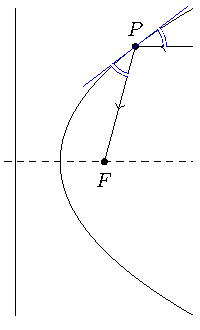
\includegraphics[width=\textwidth]{../Diagrams/Conics/parabola-cropped.pdf}
      \caption{A parabola.}
      \label{fig:parabola2}
    \end{subfigure}\hspace{0.1\textwidth}
    \begin{subfigure}{0.45\textwidth}
        \centering
        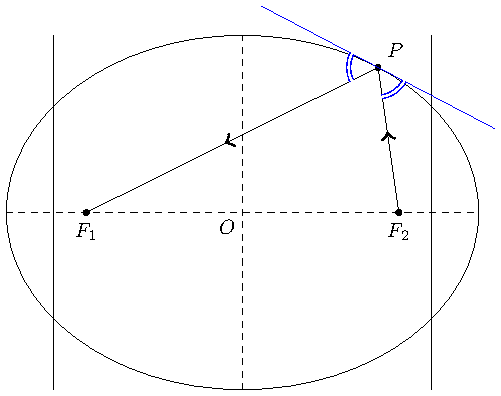
\includegraphics[width=\textwidth]{../Diagrams/Conics/ellipse.pdf}
        \caption{An ellipse.}
        \label{fig:ellipse2}
    \end{subfigure}

    \begin{subfigure}{0.45\textwidth}
      \centering
      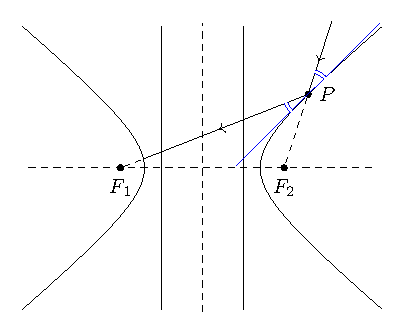
\includegraphics[width=\textwidth]{../Diagrams/Conics/hyperbola.pdf}
      \caption{A hyperbola}
      \label{fig:hyperbola2}
  \end{subfigure}
    \caption{\ref{Me} \ref{source:conics2} The reflective property of conics, their directrices, and foci.}
    \label{fig:conics2}
  \end{figure}
  \begin{itemize}[label=\(\circ\)]
    \item Conics in polar forms. Consider a conic with a focus at the origin, and a directrix 
  \end{itemize}
  \begin{table}[H]
    \centering
    \begin{tabular}{p{1.5cm}p{1.5cm}p{1.5cm}}
      & \begin{tabular}{|p{1.5cm}|}
        \hline
        \centering Top\\
        \(y=p\)
      \end{tabular} &\\
      \begin{tabular}{|p{1.5cm}}
        \hline
        \centering Left\\
        \(x=-p\)
      \end{tabular} &
      \begin{tabular}{|p{1.5cm}|}
        \hline
        \centering \vphantom{Top}\\
        \(\vphantom{y=p}\)
      \end{tabular} & 
      \begin{tabular}{p{1.5cm}|}
        \hline
        \centering Right\\
        \(x=p\)
      \end{tabular}\\
      \begin{tabular}{p{1.5cm}}
        \hline
        \centering \vphantom{Top}\\
        \(\vphantom{y=p}\)
      \end{tabular} &
      \begin{tabular}{|p{1.5cm}|}
        \hline
        \centering Bottom\\
        \(y=-p\)
      \end{tabular}
      & 
      \begin{tabular}{p{1.5cm}}
        \hline
        \centering \vphantom{Top}\\
        \(\vphantom{y=p}\)
      \end{tabular}\\
      & \begin{tabular}{p{1.5cm}}
        \hline \hphantom{1}   
      \end{tabular} &
    \end{tabular}
  \end{table}
  for some \(p>0\). In each respective case, the polar equation for the conic is given by
  \begin{table}[H]
    \centering
    \begin{tabular}{p{3cm}p{3cm}p{3cm}}
      & \begin{tabular}{|p{3cm}|}
        \hline
        \centering Top\\
        \[r=\frac{ep}{1+e\sin(\theta)}\]
      \end{tabular} &\\
      \begin{tabular}{|p{3cm}}
        \hline
        \centering Left\\
        \[r=\frac{ep}{1-e\cos(\theta)}\]
      \end{tabular} &
      \begin{tabular}{|p{3cm}|}
        \hline
        \centering \vphantom{Top}\\
        \[\vphantom{r=\frac{ep}{1+e\sin(\theta)}}\]
      \end{tabular} & 
      \begin{tabular}{p{3cm}|}
        \hline
        \centering Right\\
        \[r=\frac{ep}{1+e\cos(\theta)}\]
      \end{tabular}\\
      \begin{tabular}{p{3cm}}
        \hline
        \centering \vphantom{Top}\\
        \[\vphantom{r=\frac{ep}{1+e\sin(\theta)}}\]
      \end{tabular} &
      \begin{tabular}{|p{3cm}|}
        \hline
        \centering Bottom\\
        \[r=\frac{ep}{1-e\sin(\theta)}\]
      \end{tabular}
      & 
      \begin{tabular}{p{3cm}}
        \hline
        \centering \vphantom{Top}\\
        \[\vphantom{r=\frac{ep}{1+e\sin(\theta)}}\]
      \end{tabular}\\
      & \begin{tabular}{p{3cm}}
        \hline \hphantom{1}   
      \end{tabular} &
    \end{tabular}
  \end{table}
\end{stbox}
\begin{GCSkills}{}
  The parametric forms of the various conics can be found within the GC; no memorisation is needed!
  \begin{center}
    \texttt{apps} \(\Longrightarrow\) \texttt{2:Conics} \(\Longrightarrow\) \texttt{mode} \(\Longrightarrow\)  \texttt{PAR} \(\Longrightarrow\) \texttt{y=} \(\Longrightarrow\) 
    \begin{tabular}{Sc}
      \texttt{1:CIRCLE}\\
      \texttt{2:ELLIPSE}\\
      \texttt{3:HYPERBOLA}\\
      \texttt{4:PARABOLA}
    \end{tabular}.
  \end{center}
\end{GCSkills}
  \begin{note}
    \begin{itemize}[label=\(\circ\)]
      \item The area of an ellipse is given by \(\pi ab\).
      \item The \emph{major/minor axes} of an ellipse refer to the longest/shortest diameter of the ellipse. 
      \item The \emph{semi-major/semi-minor axes} of an ellipse refer to the longest/shortest radius of the ellipse. 
      \item A \emph{focal radius} of a conic is the distance from a point on the conic to a focus of the conic.
    \end{itemize}
  \end{note}
  \begin{note}
    Some possible things to try:
    \begin{itemize}
      \item Using \(PF_1+PF_2=2a\) to form simultaneous equations.
      \item Finding the polar form of a given conic (when \(e<1\) so \(r \geq 0\)) to solve for distances.
      \item Congruent/Similar triangles.
      \item Classic use of discriminants.
      \item \hyperlink{vieta}{Vieta's formula}.
    \end{itemize}
  \end{note}
  \begin{example}{}{}
    Describe the significance of the reflective property of parabolas in relation to the reception of the satellite TV.
    \begin{itemize}
      \item As the satellite is very far from the parabolic dish, the rays coming towards the dish can be taken to be parallel rays.
      \item These rays would all be reflected by the dish and converge at the focus. So, the receiver so should be placed at the focus to maximise the reception of the satellite TV. 
    \end{itemize}
  \end{example}
\chapter{Functions}
\begin{stbox}{General Information}
  \begin{enumerate}
    \item The horizontal line test: 
    \begin{enumerate}
      \item Fail: Since\footnote{some specific \(k\), e.g. \(y=1/2\)} \(y=k\) intersects the graph of \(y=f(x)\) more than once, therefore \(f\) is not injective.
      \item Success: Since \emph{any} horizontal line \(y=k\) will intersect the graph of \(y=g(x)\) \emph{at most once}, so \(f(x)\) is one-one.
    \end{enumerate}  
    \item The inverse function, \(f^{-1}\), of a function \(f\) exists iff \(f\) is one-one.
    \item \(y=f^{-1}\) is a reflection of \(y=f(x)\) about the line \(y=x\).
    \item The composite function \(gf\) exists iff \(R_f \subseteq D_g\).
    \item \(D_{gf}=D_f\) \& \(R_{gf}\subseteq R_g\).
    \item Finding the range:
    \begin{enumerate}
      \item Graphing method:
      \item Mapping method, e.g.: \(\begin{tikzcd}
        {D_f=(0, \infty)} & {(1,\infty)} & {(0,\infty)=R_{gf}} & {} & {}
        \arrow["f", from=1-1, to=1-2]
        \arrow["g", from=1-2, to=1-3]
      \end{tikzcd}\)
    \end{enumerate} 
  \end{enumerate}
\end{stbox}
\chapter{Permutations and Combinations}
\begin{definition}{}{}
  The terms \(n\) \emph{pick} \(r\) and \(n\) \emph{choose} \(r\) respectively denote 
  \[{^n}P_r \coloneq  \frac{n!}{(n-r)!} \qquad\text{and}\qquad \binom{n}{r}\coloneq{^n}C_r\coloneq \frac{n!}{(n-r)!r!}.\]
\end{definition}
\begin{stbox}{General Information}
  \begin{itemize}
    \item Addition and multiplication principles
    \item Know how to `bundle' objects together so as to calculate the total no. of permutations.
    \item There are 
    \[\frac{n!}{n_1!n_2!\cdots n_r!}\]
    number of ways to arrange \(n\) objects, of which \(n_i\) are similar, for each \(i\).
  \end{itemize}
\end{stbox}
    \begin{fact}
      Intuition: If there are \(n_1\) objects are non-distinct out of \(n\) objects, then there are \(n_1!\) ways to arrange these objects that results in `the same' permutation.
    \end{fact}
  \begin{stbox}{}
  \begin{itemize}
    \item Case-wise considerations/calculations (then summing together the total number of permutations)
    \item Unordered circular permutations:\\
    There are \(n!/n=(n-1)!\) number of ways of arranging \(n\) distinct objects in a circle.
  \end{itemize}
\end{stbox}
    \begin{fact}
      For unordered circular permutations, we do not care if you rotate the seating arrangement, as long as neighbours are preserved for each object. i.e. \((A,B,C,D) \sim (B,C,D,A)\). As a result, each such collection of \(n\) permutations reduces down to one. Thus, explaining the division by \(n\).
    \end{fact}
\begin{stbox}{}
\begin{itemize}
    \item Complementary Method, i.e. taking number of arrangements without restriction - number of arrangements with the opposite of that restriction.
\end{itemize}
\end{stbox}
    \begin{example}{}{}
      Number of ways two girls \emph{cannot} sit next to each other = number of arrangements \emph{without restriction} \(-\) number of arrangements with girls sitting \emph{together}.
    \end{example}
\begin{stbox}{}
\begin{itemize}
    \item Insertion Method, place down some of your objects and then insert the rest in the gaps.
  \end{itemize}
\end{stbox}
    \begin{example}{}{}
      \begin{enumerate}[label={}]
        \item Boys sit at table first: \(2!\) ways.
        \item \vspace{-1mm} From the 3 gaps, choose 2 for the 2 girls to sit at: 3 ways.
        \item \vspace{-1mm} The girls can arrange themselves in \(2!\) ways.
        \item \vspace{-1mm} So, total no. of ways is \(2! \cdot 3 \cdot 2!=12\).
      \end{enumerate}
    \end{example}
\begin{stbox}{}
\begin{itemize}
    \item Ordered circular permutations: First calculate the number of unordered permutations, then add the ordering at the end.
  \end{itemize}
\end{stbox}
    \begin{note}
      Circular arrangements are not the same as row arrangements.
      
      We know that \(A\) and \(B\) are not considered to be seating together in the row arrangement of \((A,C,D,E,B)\). But, they are seating together in a corresponding row arrangement. The number of row arrangements can be less than, equal to, or more than the number of circular arrangements.
    \end{note}
\chapter{Vectors}
\begin{note}
  A useful fact about cross products. For any \(a_i,b_i\in \mathbb{R}\):
  \[\left\lVert 
    \begin{pmatrix}
      a_1\\
      a_2\\
      a_3
    \end{pmatrix}\times
    \begin{pmatrix}
      b_1\\
      b_2\\
      b_3
    \end{pmatrix}
   \right\rVert=
  \begin{vmatrix}
    1 & a_1 & b_1\\
    1 & a_2 & b_2\\
    1 & a_3 & b_3\\
  \end{vmatrix}.\]
\end{note}
\begin{longtable}{|Sc|Sc|}
  \hline
  Lines & Planes\\
  \hline
  \multicolumn{2}{|Sc|}{Equivalent Forms}\\
  \hline
  \begin{minipage}{0.4\linewidth}
    \begin{enumerate}
      \item Vector Equation: \[\ell \colon \mathbf{r}=\mathbf{a}+\lambda \mathbf{m}\text{, }\lambda \in \mathbb{R},\]
      \item Cartesian Equation: 
      \[\frac{x-a_1}{m_1}=\frac{y-a_2}{m_2}=\frac{z-a_3}{m_3.}\]
    \end{enumerate}
\end{minipage} & 
\begin{minipage}{0.4\linewidth}
\begin{enumerate}
  \item Vector Equation: 
  \[\Pi \colon \mathbf{r}=\mathbf{a}+\lambda
  \mathbf{m_1}+\mu \mathbf{m_2},\ \lambda,\mu\in\mathbb{R}.\]
  \item Scalar Product Form: 
  \[\Pi \colon \mathbf{r} \cdot \mathbf{n}=p\]
  where the scalar \(p\coloneq  \mathbf{a}\cdot \mathbf{n}\),
  \item Cartesian Equation:
  \[n_1x+n_2x+n_3z=p\]
  where the normal vector\\
  \(\mathbf{n}\coloneq \begin{pmatrix}
    n_1 & n_2 & n_3
  \end{pmatrix}^\top\).
\end{enumerate}
\end{minipage}\\
\hline
\multicolumn{2}{|Sc|}{Foot of Perpendicular}\\
\hline
\begin{minipage}{0.4\linewidth}
  \begin{enumerate}
    \item[M1:] 
    \begin{enumerate}
      \item \(\overrightarrow{ON}=\mathbf{a}+\lambda \mathbf{m}\),
      \item \(\overrightarrow{QN} \cdot \mathbf{m}=0\), solve for \(\lambda\),
      \item Substitute \(\lambda\) into (a).
    \end{enumerate}
    \item[M2:] 
    \begin{enumerate}
      \item \(\overrightarrow{AN}=\left(\overrightarrow{AQ} \cdot \mathbf{\widehat{m}}\right)\mathbf{\widehat{m}}\),
      \item \(\overrightarrow{ON}=\overrightarrow{OA}+\overrightarrow{AN}\).
    \end{enumerate}
  \end{enumerate}
\end{minipage} & 
\begin{minipage}{0.4\linewidth}
  \begin{enumerate}
    \item[M1:]
    \begin{enumerate}[label=(\alph*)]
      \item \(\overrightarrow{ON}=\overrightarrow{OQ}+\lambda\mathbf{n}\),
      \item \(\overrightarrow{ON}\cdot\mathbf{n}=p\), solve for \(\lambda\),
      \item  Substitute \(\lambda\) into (a).
    \end{enumerate}
    \item[M2:]
    \begin{enumerate}[label=(\alph*)]
      \item \(\overrightarrow{QN}=\left( \overrightarrow{QA}\cdot\widehat{\mathbf{n}} \right)\widehat{\mathbf{n}}\),
      \item \(\overrightarrow{ON}=\overrightarrow{OQ}+\overrightarrow{QN}\).
    \end{enumerate}
  \end{enumerate}
\end{minipage}\\
\hline
\newpage
\hline
\multicolumn{2}{|Sc|}{Shortest Distance of Point To Line, \(QN\)}\\
\hline
\begin{minipage}{0.4\linewidth}
  \begin{enumerate}
    \item[M1:] \(\norm{\overrightarrow{AQ} \times \mathbf{\widehat{m}}}\).
    \item[M2:]
    \begin{enumerate}
      \item \(AN= \norm{\overrightarrow{AQ}\cdot \mathbf{\widehat{m}}} \),
      \item Pythagoras' Theorem.
    \end{enumerate}
    \item[M3:] Using the foot of perpendicular, find distance \(QN\).
  \end{enumerate}
\end{minipage} &
\begin{minipage}{0.4\linewidth}
  \begin{enumerate}
    \item[M1:] \(\norm{\overrightarrow{AQ}\cdot \mathbf{\widehat{n}}} \).
    \item[M2:] Distance of plane to \emph{origin}: 
    
    If \(\Pi \colon \mathbf{r}\cdot \mathbf{n}=p\), then \(\dfrac{p}{\norm{\mathbf{n}}}\) is the shortest distance from the origin to the plane \(\Pi\). 
    
    \emph{Note:}
    \begin{itemize}
      \item If \(\dfrac{p}{\norm{\mathbf{n}}}>0\), then \(\Pi\) is `above' the origin.
      \item If \(\dfrac{p}{\norm{\mathbf{n}}}<0\), then \(\Pi\) is `below' the origin.
    \end{itemize}
    \item[M3:] Using the foot of perpendicular, then find distance \(QN\).
  \end{enumerate}
\end{minipage}\\
\hline
The Relationship Between Two Lines & The Relationship Between Two Planes\\
\hline
\begin{minipage}{0.4\linewidth}
  \begin{enumerate}
    \item Parallel, Non-Intersecting
    \begin{enumerate}
      \item \(\mathbf{m_1}\newparallel \mathbf{m_2}\),
      \item Solving \(\mathbf{r_1}=\mathbf{r_2}\) gives no real solution. Or, show that \(\mathbf{a_1}\) does not lie in \(\ell_2\).
    \end{enumerate}
    \item Parallel, Coinciding
    \begin{enumerate}
      \item \(\mathbf{m_1}\newparallel \mathbf{m_2}\),
      \item \(\mathbf{a}\) lies in \(\ell_1\) and \(\ell_2\).
    \end{enumerate}
    \item Non-Parallel, Intersecting
    \begin{enumerate}
      \item \(\mathbf{m_1}\) not \(\newparallel \mathbf{m_2}\),
      \item Solve \(\mathbf{r_1}=\mathbf{r_2}\) to find intersection.
    \end{enumerate} 
    \item Skew Lines\\
    (Non-Parallel, Non-Intersecting)
    \begin{enumerate}
      \item \(\mathbf{m_1}\) not \(\newparallel \mathbf{m_2}\),
      \item Solving \(\mathbf{r_1}=\mathbf{r_2}\) gives no real solution. 
    \end{enumerate}
  \end{enumerate}
\end{minipage} &
\begin{minipage}{0.4\linewidth}
  \begin{enumerate}
    \item Distinct Parallel Planes: 
    \begin{enumerate}
      \item Show that \(\mathbf{n_1}\newparallel\mathbf{n_2}\),
      \item Find a vector \(\mathbf{b}\) for which
      \begin{enumerate}[label=(\roman*)]
        \item \(\mathbf{b}\cdot \mathbf{n_1}= p_1\),
        \item \(\mathbf{b}\cdot \mathbf{n_2}\neq p_2\).
      \end{enumerate}
    \end{enumerate}
    \item Same Plane:
    \begin{enumerate}
      \item Show that \(\mathbf{n_1}\newparallel\mathbf{n_2}\),
      \item Find a vector \(\mathbf{b}\) for which
      \begin{enumerate}[label=(\roman*)]
        \item \(\mathbf{b}\cdot \mathbf{n_1}= p_1\),
        \item \(\mathbf{b}\cdot \mathbf{n_2}= p_2\).
      \end{enumerate}
    \end{enumerate}
    \item Intersect in a line \(\ell\); To find this line:
    \begin{enumerate}[label=M\arabic*:]
      \item \(\mathbf{n_1}\times \mathbf{n_2}\) gives the direction vector. So find a common point with simultaneous equations.
      \item Solving system of linear equations, from the \emph{cartesian} form of the planes, using G.C.
    \end{enumerate}
  \end{enumerate}
\end{minipage}\\
\hline
\newpage
\hline
\multicolumn{2}{|Sc|}{The Relationship Between A Line and A Plane}\\
\hline 
\multicolumn{2}{|Sc|}{
\begin{minipage}{0.8\linewidth}
  \begin{enumerate}
    \item \(\ell\) lies in \(\Pi\)
    \begin{enumerate}[label=M\arabic*:]
      \item
      \begin{enumerate}
        \item Show \(\mathbf{m}\cdot \mathbf{n}=0\) so \(\ell \newparallel \Pi\).
        \item Then \(\mathbf{a}_\ell\cdot \mathbf{n}=p\) tells us \(\ell\) lies in \(\Pi\).
      \end{enumerate}
      \item Substitute \(\ell\) into \(\Pi\) and show the system (of lin eqns) is consistent for all \(\lambda\).
    \end{enumerate}
    \item \(\ell \newparallel \Pi\) but nonintersecting
    \begin{enumerate}[label=M\arabic*:]
      \item 
      \begin{enumerate}
        \item Show \(\mathbf{m}\cdot \mathbf{n}=0\) so \(\ell \newparallel \Pi\).
        \item Then \(\mathbf{a}_\ell\cdot \mathbf{n} \neq p\) tells us \(\ell\) and \(\Pi\) are nonintersecting.
      \end{enumerate}
      \item Substitute \(\ell\) into \(\Pi\), and show the system (of lin eqns) is inconsistent.
    \end{enumerate} 
    \item Intersect at one point
    \begin{enumerate}
      \item Check that \(\mathbf{m}\cdot \mathbf{n} \neq 0\).
      \item Then, to find the point of intersection of the plane \(\Pi\colon \mathbf{r}\cdot \mathbf{n}=p\) with the line \(\ell\colon \mathbf{r}=\mathbf{a}+\lambda \mathbf{m}\),
      we solve for \(\lambda\) using simultaneous equations or G.C.
    \end{enumerate}
  \end{enumerate}
\end{minipage}}\\
\hline
\multicolumn{2}{|Sc|}{The Point of Reflection}\\
\hline
\multicolumn{2}{|Sc|}{  
\begin{minipage}{0.8\linewidth}
\begin{center}
  \begin{enumerate}
    \item Find foot of perpendicular \(\overrightarrow{ON}\)
    \item Notice \(\overrightarrow{OA'}=\overrightarrow{OA}+2\overrightarrow{AN}=2\overrightarrow{ON}-\overrightarrow{OA}\).
  \end{enumerate}
\end{center}
\end{minipage}}\\
\hline
  \multicolumn{2}{|Sc|}{Angle Between}\\
  \hline
  \multicolumn{2}{|Sc|}{
    \begin{tabular}{Sc|Sc|Sc}
      \begin{minipage}{0.267\linewidth}
        \centering
        Two Lines
      \end{minipage} &
      \begin{minipage}{0.267\linewidth}
        \centering
        Line and Plane
      \end{minipage} &
      \begin{minipage}{0.267\linewidth}
        \centering
        Two Planes
      \end{minipage}\\
    \end{tabular}}\\
    \hline
    \multicolumn{2}{|Sc|}{
    \begin{tabular}{Sc|Sc|Sc}
      \begin{minipage}{0.267\linewidth}\vspace{-0.5cm}
        \[\theta=\cos^{-1}\left\lvert \mathbf{\widehat{m}_1}\cdot {\mathbf{\widehat{m}_2}}\right\rvert.\]
      \end{minipage} &
      \begin{minipage}{0.267\linewidth}\vspace{-0.5cm}
        \[\theta=\sin^{-1}\left\lvert \mathbf{\widehat{m}}\cdot \mathbf{\widehat{n}} \right\rvert .\]
      \end{minipage} &
      \begin{minipage}{0.267\linewidth}\vspace{-0.5cm}
        \[\theta=\cos^{-1}\left\lvert \mathbf{\widehat{n}_1}\cdot \mathbf{\widehat{n}_2} \right\rvert.\]
      \end{minipage}\\
    \end{tabular}}\\
    \hline
\end{longtable}
\begin{note}
  Describe the line \(\ell\colon\mathbf{r}=\mathbf{a}+\lambda\mathbf{m},\lambda\in \mathbb{R}\) geometrically.
  \begin{center}
    \parbox{0.9\textwidth}{
      It is the line \emph{passing through the fixed point} with position vector \(\mathbf{a}\) and is \emph{parallel to} \(\mathbf{m}\). 
    }
  \end{center}
\end{note}
\begin{note}
  Let \(\pi\) be a plane containing the line \(\ell\) and \(P\) be a point. The foot of perpendicular of \(P\) on \(\pi\) is not necessarily the same as the foot of perpendicular of \(P\) on \(\ell\). 
\end{note}
\begin{note}
  When finding the plane \(\pi\) that is `above' another plane \(\Pi\colon \mathbf{r}\cdot \mathbf{n}=p\) by a constant \(q\) units, take note of the direction of \(\mathbf{n}=
  \begin{pmatrix}
    n_1 & n_2 & n_3
  \end{pmatrix}^{\top}\). If \(n_3>0\), then \(\mathbf{n}\) is pointing `upwards'. So, \(\pi\colon \mathbf{r}\cdot\widehat{\mathbf{n}}=\highlight[green!50]{+}q\). Otherwise \(n_3<0\), meaning \(\mathbf{n}\) is pointing `downwards'. Hence, \(\pi\colon \mathbf{r}\cdot\widehat{\mathbf{n}}=\highlight[green!50]{-}q\).
  \footnotetext[0]{I'm slightly skeptical that Cambridge will not make clear which side is considered `upwards/downwards'. But, just in case, this is a good point to note.}
\end{note}
\chapter{Probability}
\begin{stbox}{General Information}
  \begin{enumerate}
    \item Principle of Inclusion and Exclusion for
    \begin{enumerate}
      \item Two events:
      \[\Prob(A \cup B)=\Prob(A)+\Prob(B)-\Prob(A \cap B),\]
      \item Three events:
      \[\Prob(A \cup B \cup C)=\Prob(A)+\Prob(B)+\Prob(C)-\Prob(A\cap B)-\Prob(A \cap C)-\Prob(B \cap C)+\Prob(A \cap B \cap C).\]
    \end{enumerate}
    \item Mutually Exclusive Events:
    \begin{align*}
      \Prob(A \cap B)&=0,\\
      \Prob(A \cup B)&=\Prob(A)+\Prob(B).
    \end{align*}
    \item Independent Events:
    \begin{align*}
      \Prob(A \,\vert\, B)&=\Prob(A),\\
      \Prob(A \cap B)&=\Prob(A)\Prob(B).
    \end{align*}
    \item Conditional Probability:
    \[\Prob(A \,\vert\, B)=\frac{\Prob(A \cap B)}{\Prob(B)}.\]
    \item Use PnC to help compute stuff faster.
    \item When we want to find the greatest and least possible probability (e.g. of \(\Prob(A^\complement\cap B^\complement\cap C^\complement)\)), it is advisable to draw a Venn diagram and fill in all relevant probabilities. 
  \end{enumerate}
\end{stbox}
\begin{example}{}{}
  There are 6 white balls and 5 black balls. Two are randomly drawn. What is the probability that one is white and the other black?
  \begin{align*}
    \left(\frac{5}{11}\right)\left(\frac{6}{10}\right)+\left(\frac{6}{11}\right)\left(\frac{5}{10}\right)=\frac{6}{11} \qquad&\text{vs}\qquad \frac{\binom{6}{1}\binom{5}{1}}{\binom{11}{2}}=\frac{6}{11}.
  \end{align*}
\end{example}
\chapter{Differential Equations}
\section{First Order D.E.s}
\subsection{Elementary Solving Techniques}
\begin{stbox}{General Information}
  \begin{itemize}
    \item Separable Variables:
    \begin{align*}
      \frac{dy}{dx}&=f(y)g(x),
      \int \frac{1}{f(y)}\,dy=\int g(x)\,dx.
    \end{align*}
    \item Integrating Factor:
    \begin{align*}
      \frac{dy}{dx}+P(x)y&=Q(x),\quad\text{let I.F.}=e^{\int P(x)\,dx}\\
      e^{\int P(x)\,dx} \frac{dy}{dx}+ye^{\int P(x)\,dx}P(x)&=Q(x)e^{\int P(x)\,dx},\\
      ye^{\int P(x)\,dx}&=\int Q(x)e^{\int P(x)\,dx}\,dx.
    \end{align*}
  \end{itemize}
\end{stbox}
\begin{example}{Justification for D.E. models of real world scenarios}{}
  Consider the proportion \(u\) of susceptible individuals --- those who have not yet caught the disease --- and the proportion \(v\) of infected individuals and the proportion \(w\) of recovered individuals. The standard model used in measuring the rate of spread of the disease assumes that \(du/dt=-kuv\), where \(k\) is a positive constant; the unit of time used is the average length of time for which a person is infected.
  \begin{enumerate}[label=(\alph*)]
    \item Describe the relevance of each bracketed term in the equation \(du/dt=(-k)(uv)\) in terms of the spread of the disease.
    \item Justify the assertion that \(dw/dt\approx v\).
  \end{enumerate}
  \rule{20cm-137.0549pt}{0.05mm} 
  \begin{enumerate}[label=(\alph*)]
    \item The \(uv\) term measures the interaction between susceptibles and infected. This should be directly proportional to \(du/dt\): When interactions between susceptibles and infected are more common (\(uv>0\) is larger), more susceptibles should become infected (\(du/dt\) is more negative). The proportionality constant \(-k\) between \(uv\) and \(du/dt\) is negative to illustrate this relationship; the proportion of susceptibles cannot increase when population size is constant.   
    \item Since the unit of time used in the model is the average length of time for which a person is infected, if there are \(I\) infected individuals at time \(t\), then after one unit time, roughly \(I\) people would have recovered. i.e. \(dR/dt\approx I\) so \(dw/dt\approx v\), where \(R\) is the number of people who have recovered.
  \end{enumerate}
\end{example}
\subsection{Numerical Methods}
\begin{stbox}{General Information}
  \begin{itemize}
    \item Euler's Method: 
    \[y_{i+1}=y_i+hf(x_i,y_i),\text{ where }x_n=x_0+nh.\]
    We can present our working directly, as shown in Example 17.1, if there are only one or two iterations. Otherwise, draw the following table.
    \begin{table}[H]
      \centering
      \begin{tabular}{|Sc|Sc|Sc|}
        \hline
        \(x\) & \(y\) & \(y+hf(x,y)\)\\
        \hline
        \(x_0\)& \(y_0\) & \(y_1\)\\
        \hline
        % \(x_0+h\)& \(y_1\) & \(y_2\)\\
        % \hline
        \(\vdots\) & \(\vdots\) & \(\vdots\)\\
        \hline
        \(x_n\) & \(y_n\) &\\
        \hline
      \end{tabular}
      \caption{Tabular presentation for Euler's Method.}
      \label{table:euler-presentation}
    \end{table}
  \end{itemize}
\end{stbox}
    \begin{example}{}{}
      Let (step size) \(h=0.25\) and \(f(x,y)=\frac{dy}{dx}\):
      \begin{align*}
        \text{By MF26,}\quad y_2&=\frac{2}{3}+hf\left(0,\frac{2}{3}\right)\\
        &=\frac{13}{18}\\[3mm]
        y_3&=\frac{13}{18}+hf\left(0.25,\frac{13}{18}\right)\\
        &=0.6701865657.\\[3mm]
        \text{Therefore, }y(0.5)&\approx 0.670.
      \end{align*}
    \end{example}
    \begin{stbox}{}
      \setcounter{enumi}{1}
    \begin{itemize}
    \item Improved Euler's Method: 
    \[u_{i+1}=y_i+hf(x_i,y_i)\quad\&\quad y_{i+1}=y_i+\frac{h}{2}[f(x_i,y_i)+f(x_{i+1},u_{i+1})].\]
    Usually only one or two iterations is necessary, so presenting our working directly is sufficient.
% \end{itemize}
% \begin{itemize}
    \item Error:
    \begin{enumerate}
      \item If \(\frac{dy}{dx}\) can be shown to be \emph{increasing} from the calculations of \(f(x,y)\), then the curve is \emph{concave upwards}, leading to a \emph{underestimate}.
      \item If \(\frac{dy}{dx}\) can be shown to be \emph{decreasing} from the calculations of \(f(x,y)\), then the curve is \emph{concave downwards}, leading to a \emph{overestimate}.
    \end{enumerate}
  \end{itemize}
\end{stbox} ~
\begin{example}{}{}
  From the computation, \emph{the values of} \(\frac{dy}{dx}\) \emph{increases}, i.e. \(\frac{d^2y}{dx^2}>0\), implying that the solution curve is \emph{concave upwards}. Therefore, we have an \emph{underestimation}. 
\end{example}
\begin{example}{}{}
  It is suggested that the estimation in part (ii)\footnote{Given the point (1,1), we estimated the value of y(2) using the Improved Euler's Method} can be further improved by reducing the step size. Sketch the solution curve and hence comment on this suggestion.\\[3mm]
  The solution curve has a \emph{stationary point at} \(x=1.47\), which is between 1 and 2 and also the gradient of the curve is close to zero for \(x\) value beyond this stationary point. Thus, when the step size is reduced, \emph{tangent} at point close to this stationary point becomes \emph{almost parallel} to the curve, making \emph{little improvement} to the estimation due to \emph{little difference in} \(y\). 
\end{example}
\begin{example}{}{}
  It is found that the approximation obtained in (i) for the \(y\)-coordinate where \(x=0.75\) is an underestimation and has a percentage error of 120.633\%. Explain why there is such a substantial error.\\[3mm]
  From gradient values calculated above, we suspect sharp charges in gradient values within the interval (from negative to positive). Yet \emph{Euler's Method\footnote{We are explaining what it does} simply uses a straight line segment} with gradient\footnote{Emphasising negative gradient (Show its value)} \(-4.6409\) to estimate the curve for the first iteration, which could have lead to a significant underestimation of the \(y\)-value.
\end{example}
\begin{note}{}{}
  Compare the relative merits of Euler's Method and the Improved Euler's Method.
  \begin{enumerate}[wide=0pt, leftmargin=*]
    \item[Euler's Method:] It is computationally simpler.
    \item[Improved Euler's Method:] It is More accurate as it takes the mean of the initial and next gradient. 
  \end{enumerate}
\end{note}
\begin{figure}[H]
  \centering
  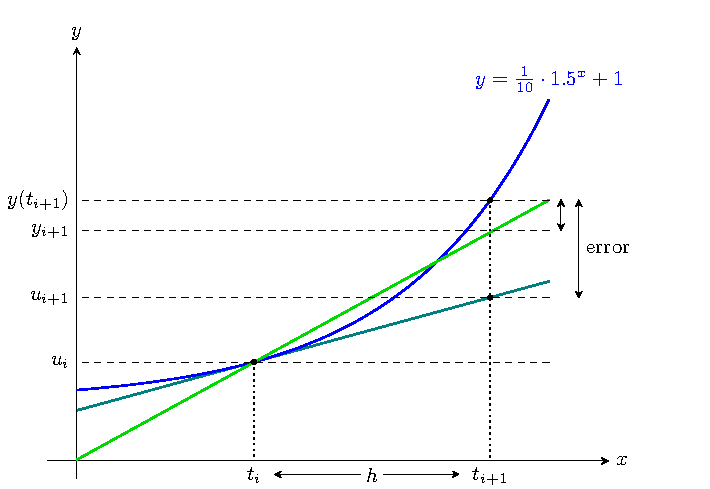
\includegraphics{../Diagrams/Euler's-Methods/euler's-method.pdf}
  \caption{\ref{source:euler's-methods} An illustration of \textcolor{green!50!blue}{Euler's Method} and the \textcolor{green!85!black}{Improved Euler's Method}.}
  \label{fig:euler's-methods}
\end{figure}
\begin{note}
  To find the percentage difference of the true value and the estimated value, we calculate
  \[\frac{\text{true value}-\text{estimated value}}{\text{true value}}\cdot 100\%.\]
\end{note}
\begin{note}
  Explain the large discrepancy between the approximations yielded by Euler's Method and the Improved Euler's Method.
  \begin{itemize}
    \item There is a large increase in the gradient of the curve from [the value of \(y'(a)\)] at \(x=a\) to [the value of \(y'(b)\)] at \(x=b\). 
    \item So, the average of the two gradients used in the Improved Euler's Method is significantly larger than [the value of \(y'(a)\)] used in Euler's Method.
    \item Hence, a large discrepancy between the results of the two methods is observed.
  \end{itemize}
\end{note}
\begin{note}
  State the condition when the Improved Euler's Method is not an improvement over Euler's Method
  \begin{center}
    When the gradient function is a constant throughout the allocated interval.
  \end{center} 
\end{note}
\begin{example}{Comparing three sets of approximations.}{}
  \begin{enumerate}[label=(\roman*)]
    \item Obtain the solution of the differential equation 
    \[\frac{dy}{dx}-y=x\]
    given that \(y=0\) when \(x=0\). Obtain, correct to 3 significant figures, the values of \(y\) when \(x=0.1\) and \(x=0.2\).
  \end{enumerate}
  Now consider the differential equation
  \[\frac{dy}{dx}-\sin(y)=x,\]
  where \(x=0\) when \(x=0\).
  \begin{enumerate}[label=(\roman*)]
    \setcounter{enumi}{1}
    \item Use Euler's Method with step length 0.1 to estimate the values of \(y\) when \(x=0.1\) and \(x=0.2\).
    \item Use the improved Euler Method with step length 0.1 to estimate the values of \(y\) when \(x=0.1\) and \(x=0.2\).
    \item Comment on your numerical answers from parts (i), (ii), and (iii). \hspace*{\fill} [2]
  \end{enumerate}
  \rule{20cm-137.0549pt}{0.05mm}
  \begin{enumerate}[label=(\roman*)]
    \item \(y(0.1)=0.00517\) and \(y(0.2)=0.0214\).
    \item \(y(0.1)\approx 0\) and \(y(0.2)\approx 0.01\).
    \item \(y(0.1)\approx 0.005\) and \(y(0.2)\approx 0.210\).
    \item 
    \begin{itemize}
      \item Since the values of \(y\) are small, \(\sin(y)\approx y\) by small angle approximation. \hspace*{\fill} [1]
      \item Hence, the values of \(y\) from (i) can be compared with estimates from (ii) and (iii). 
      \item Since the answers from (iii) are closer to those in (i) than the those in (ii), the answers in (iii) are more accurate estimates of the exact values of \(y\). \hspace*{\fill} [1]
    \end{itemize}
  \end{enumerate}
\end{example}
\begin{example}{}{}
  The function \(y=y(x)\) satisfies \(\frac{dy}{dx}=\frac{1}{10}(\sin(x)-xy)\). 
  \begin{enumerate}[label=(\roman*)]
    \item The value of \(y(h)\) is to be found, where \(h\) is a small positive number, and \(y(0)=0\).
    \begin{enumerate}
      \item Use two steps of Euler's method to determine an approximation to \(y(h)\) in terms of \(h\).
      \item Use one step of the improved Euler formula to find alternative solutions to \(y(h)\) in terms of \(h\).
    \end{enumerate}
    \item \textcolor{yellow}{\(\bigstar\)} Show that \(y=y(x)\) satisfies \(e^{0.05h^2}y(h)=\int_{0}^{h}0.1e^{0.05x^2}\sin(x)\,dx\).
    % \begin{align*}
    %   \frac{dy}{dx}&=\frac{1}{10}[\sin(x)-xy]\\
    %   \frac{dy}{dx}+\left( \frac{1}{10}x \right)&=\frac{1}{10}\sin(x)\\
    %   \text{Let I.F. be }e^{\int\frac{1}{10}x\,dx}&=e^{0.05x^2}:\\
    %   e^{0.05x^2}y&=\int\frac{1}{10}e^{0.05x^2}\sin(x)\,dx\\
    %   \left[e^{0.05x^2}y\right]_{0}^{h}&=\int_{0}^{h}\frac{1}{10}e^{0.05x^2}\sin(x)\,dx\\
    %   e^{0.05h^2}y(h)-e^0y(0)&=\int_{0}^{h}\frac{1}{10}e^{0.05x^2}\sin(x)\,dx\\
    %   \text{Since y(0)=0},\\
    %   e^{0.05h^2}y(h)&=\int_{0}^{h}\frac{1}{10}e^{0.05x^2}\sin(x)\,dx.
    % \end{align*}
    \begin{proof}
      We see that
      \begin{align*}
        \frac{dy}{dx}&=\frac{1}{10}[\sin(x)-xy]\\
        \frac{dy}{dx}+\left( \frac{1}{10}x \right)&=\frac{1}{10}\sin(x)\\
        \intertext{Let I.F. be \(e^{\int\frac{1}{10}x\,dx}=e^{0.05x^2}\):}
        e^{0.05x^2}y&=\int\frac{1}{10}e^{0.05x^2}\sin(x)\,dx\\
        \left[e^{0.05x^2}y\right]_{0}^{h}&=\int_{0}^{h}\frac{1}{10}e^{0.05x^2}\sin(x)\,dx\\
        e^{0.05h^2}y(h)-e^0y(0)&=\int_{0}^{h}\frac{1}{10}e^{0.05x^2}\sin(x)\,dx\\
        \shortintertext{Since \(y(0)=0\),}
        e^{0.05h^2}y(h)&=\int_{0}^{h}\frac{1}{10}e^{0.05x^2}\sin(x)\,dx.
      \end{align*}
    \end{proof}
    \item Use the fact that \(h\) is small to estimate \(\int_{0}^{h}0.1e^{0.05x^2}\sin(x)\,dx\). Hence find another approximation to \(y(h)\) in terms of \(h\).
    \item \textcolor{yellow}{\(\bigstar\)} Discuss the relative merits of the three methods employed to obtain these approximations.
  \end{enumerate}
  \begin{itemize}
    \item Two step of Euler's method might be lead to a more accurate approximation than one step of the improved Euler method, because of the larger number of steps.
    \item The improved Euler method might lead to a more accurate approximation, as it takes the mean of the gradients \(y'(0)\) and \(y'(h)\), rather than the simplistic tangent line approximation used by Euler's method.
    \item The method in (iii) might be more accurate than Euler's method and the improved Euler method, because it uses quadratic polynomials/an exponential curve\footnote{It depends on how you calculated the approximation to \(y(h)\) in (iii).} instead of straight line segments.
  \end{itemize}
\end{example}
\section{Second Order D.E.}
\begin{center}
  \begin{tabular}{|Sc|Sc|}
    \hline
    \multicolumn{2}{|Sc|}{\textbf{Homogenous}}\\
    \hline
    Roots & Solution \(y_c\)\\
    \hline
    \(m_1 \neq m_2\) & \(y=Ae^{m_1x}+Be^{m_2x}\)\\
    \hline
    \(m\coloneq m_1=m_2\) & \(y=(Ax+B)e^{mx}\)\\
    \hline
    \(m=\highlight[red!30]{p} \pm qi\) & \(y=e^{\highlight[red!30]{p}x}(A \cos(qx)+B \sin(qx))\)\\
    \hline
    \multicolumn{2}{|Sc|}{\textbf{Non-Homogenous, }\(c_2 \dfrac{d^2y}{dx^2}+c_1 \dfrac{dy}{dx}+c_0y=f(x)\)}\\
    \hline
    \multicolumn{2}{|Sc|}{\(y=y_c+y_p\) (C.F. + P.I.)}\\
    \hline
    \(f(x)\) & Trial Function for P.I.\\
    \hline
    Degree \(n\) polynomial & \(y_p=\sum\limits_{i=0}^{n}a_ix^i\)\\
    \hline
    \(\alpha e^{kx}\) & \(y_p=ae^{kx}\)\\
    \hline
    \(\alpha \cos(kx) +\beta \sin(kx)\) & \(y_p=a\cos(kx)+b\sin(kx)\)\\
    \hline
  \end{tabular}
  \begin{note}
    If \(y_c\) and \(f(x)\) share some common term, then \(y_p\) should be multiplied by \(x\) (some least \(i \in \mathbb{N}\) times till \(x^iy_p\) has no common term with \(y_c\)).  
  \end{note}
  \begin{example}{}{}
    \begin{enumerate}
      \item If \(y_c=Ae^{-3x}\) and \(f(x)=10e^x\), then \(y_p=ke^x\)
      \item If \(y_c=Ae^x+Be^{-3x}\) and \(f(x)=10e^x\), then \(y_p=kxe^x\).
      \item If \(y_c=Ae^x+Bxe^{x}+Ce^{-3x}\) and \(f(x)=10e^x\), then \(y_p=kx^2e^x\).
    \end{enumerate}
  \end{example}
\end{center}
\begin{note}\hypertarget{R-formulas}{}
  \(R\)-formulas. Let \(a,b\in \mathbb{R}\). Then, for 
  \[R\coloneq\sqrt{a^2+b^2} \qquad\text{and}\qquad \tan(\alpha)\coloneq\frac{b}{a},\]
  we have that
  \[a\sin(\theta)+b\cos(\theta)=R\sin(\theta+\alpha) \qquad\text{and}\qquad b\sin(\theta)+a\cos(\theta)=R\cos(\theta-\alpha).\]
\end{note}
\section{Applications}
\subsection{Exponential Growth}
\begin{stbox}{General Information}
  Let \(k\) be the \emph{per-capita growth rate}\footnote{i.e. after accounting for births and deaths.} and \(P(t)\) be the population at time \(t\). Then we have the model:
  \[\frac{dP}{dt}=kP,\]
  with the solution
  \[P(t)=P_0e^{kt}.\]
\end{stbox}
\subsection{Logistics Growth}
\begin{stbox}{General Information}
  Let \(k\) be the \emph{per-capita growth rate}\footnote{i.e. after accounting for births and deaths.}, \(P(t)\) be the population at time \(t\), and \(N\) be the \emph{carrying capacity} of the system. Then we have the model:
  \[\frac{dP}{dt}=kP\left(1-\frac{P}{N}\right).\]
  \begin{enumerate}
    \item Without solving the logistics equation, we can sketch the solution curve by noting the sign of \(dP/dt\):
    \begin{enumerate}
      \item Equilibrium population values occur at \(P=0\) and \(P=N\).
      \item If, for instance \(k>0\),
      \begin{enumerate}[wide=0pt, leftmargin=*]
        \item[\(0<p<N\):] \(1-\frac{P}{N}>0\) so \(dP/dt>0\),
        \item[\(P>N\):] \(1-\frac{P}{N}<0\) so \(dP/dt<0\).  
      \end{enumerate}
    \end{enumerate}
    ``As \(t\) increases,  the population of \rule{1cm}{0.1mm}  increases to the stable population of \rule{1cm}{0.1mm}.''
  \end{enumerate}
\end{stbox}
\begin{example}{Neat trick of letting \(A=\pm \text{constant}\)}{}
  \begin{align*}
    \frac{dP}{dt}&=3P\left(1-\frac{P}{200}\right),\\
    \int \frac{1}{3P}+\frac{1}{600-3P}\,dP &= \int 1 \,dt,\\
    \ln \abs{\frac{3P}{600-3P}}&=3t+3c,\\
    \frac{3P}{600-3P}&=Ae^{3t}\text{, where }\highlight[red!30]{A=\pm e^{3c}},\\
    P&=\frac{200A}{A+e^{-3t}}
  \end{align*}
\end{example}
\begin{figure}[H]
  \centering
  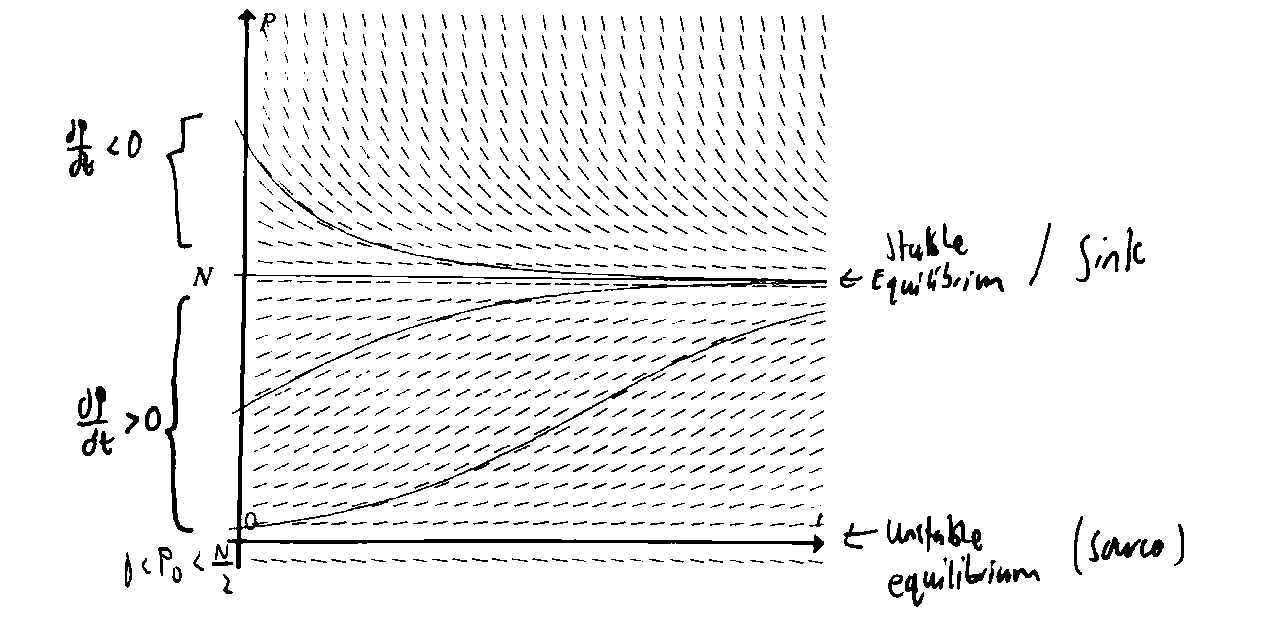
\includegraphics[width=0.35\textwidth]{Logistics Curve}
  \caption{\ref{Me} Logistics Curve}
  \label{fig:logistics-curve}
\end{figure}
\subsection{Harvesting}
\begin{stbox}{General Information}
  Let \(k\) be the \emph{per-capita growth rate}, \(P(t)\) be the population at time \(t\), \(N\) be the \emph{carrying capacity} of the system, and \(H\) the constant \emph{harvesting rate}. Then we have the model:
  \[\frac{dP}{dt}=kP\left(1-\frac{P}{N}\right)-H.\]
\begin{enumerate}
  \item Bifurcation Point
  \begin{enumerate}
    \item When \(0 \leq H<\frac{kN}{4}\), there are two equilibrium points, \(P=\frac{N}{2}\pm \sqrt{\frac{N^2}{4}-\frac{HN}{k}}\).
    \item When \(H=\frac{kN}{4}\), there is one equilibrium point at \(P=\frac{N}{2}\) (the bifurcation point).
    \item When \(H>\frac{kN}{4}\), there is no equilibrium point
  \end{enumerate}
  \item For Non-Extinction: 
  \begin{align*}
    \quad\frac{N^2}{4}-\frac{HN}{k} \geq 0 \qquad\text{and}\qquad P_0 \geq \frac{N}{2}-\sqrt{\frac{N^2}{4}-\frac{HN}{k}}.
  \end{align*}
\end{enumerate}
\end{stbox}

\subsection{Physics}
\begin{stbox}{General Information}
  \textbf{MUST} rmb the forms.
  \begin{enumerate}
    \item Spring System (where \(k>0\) is the spring constant) 
    \[\ddot{x}+\frac{k}{m}x=0.\]
    Solution: use \(\highlight[red!30]{\text{R-formula}}\) to convert to \(A \cos(\omega t + \phi)\) where angular frequency \(\omega=\sqrt{k/m}\). Period \(T=2\pi/\omega=2\pi \sqrt{m/k}\).
    \item Simple Pendulum (where \(\ell\) is its length)
    \[\ddot{x}+\frac{g}{\ell}x=0.\]
    Angular frequency \(\omega=\sqrt{g/\ell}\) and period \(T=2\pi \sqrt{\ell/g}\).
    \item Spring-Mass-Dashpot System (where \(c>0\) is the damping constant)
    \[\ddot{x}+\frac{c}{m}\dot{x}+\frac{k}{m}x=0.\]
    Solution
    \begin{enumerate}
      \item Real and Distinct Roots: \emph{Overdamped}
      \item Identical Real Roots: \emph{Critically Damped}
      \item Complex Conjugate Roots: \emph{Underdamped}\\
      \emph{``It will oscillate about the equilibrium position with decreasing amplitude.''}
    \end{enumerate}
  \end{enumerate}
\end{stbox}
\begin{figure}[H]
  \centering
  \includestandalone[width=\textwidth]{../Diagrams/Oscils}
  \caption{\ref{source:oscillatory-behavior} Oscillatory behaviors.}
  \label{fig:oscillatory-behavior}
\end{figure}
\chapter{Discrete Random Variables}
\begin{stbox}{General Information}
  \begin{enumerate}
    \item Expectation / Mean, 
    \[\operatorname{E}(X)\coloneq \sum_{\text{all } x}{x\Prob(X=x)}.\]
    \item Variance 
    \[\operatorname{Var}(X)\coloneq E\hspace{-0.7mm}\left(X^2\right)-[E(X)]^2=\E{\left( (X-\mu)^2 \right)}.\]
    \item Standard Deviation
    \[\sigma\coloneq \sqrt{\operatorname{Var}(X)}.\]
    \item Properties for two \emph{independent} random \emph{variables} \(X\) and \(Y\); two \emph{independent observations} \(X_1\) and \(X_2\) of \(X\):
    \begin{enumerate}
      \item \(\operatorname{E}(aX+bY+c)=a\operatorname{E}(X)+b\operatorname{E}(Y)+c\),
      \item \(\operatorname{Var}(aX+bY+c)=a^2\operatorname{Var}(X)+b^2\operatorname{Var}(Y)\).
    \end{enumerate}
    \item Probability Distribution Table:
    \begin{table}[H]
      \centering
      \begin{tabular}{|Sc|Sc|Sc|Sc|}
        \hline
        \(x\) & 1 & \(\cdots\) & \(n\)\\
        \hline
        \(\Prob(X=x)\) & \(\Prob(X=1)\) & \(\cdots\) & \(\Prob(X=n)\)\\
        \hline
      \end{tabular}
      \caption{A probability distribution table.}
      \label{table:a-probability-distribution-table}
    \end{table}
  \end{enumerate}
\end{stbox}
\chapter{Special Discrete Random Variables}
\begin{definition}{}{}
  A discrete random variable \(X\) which takes all values in \(\mathbb{Z}^{+}_{0}\) is a \emph{binomial distribution} with probability of success \(p\), denoted by \(X \sim \operatorname{B}(n,p)\), iff
  \[\Prob(X=x)=\binom{n}{x}p^x(1-p)^{n-x}.\]
\end{definition}
\begin{definition}{}{}
  A discrete random variable \(X\) which takes all values in \(\mathbb{Z}^{+}\) has a \emph{geometric distribution} with probability of success \(p\), denoted by \(X \sim \operatorname{Geo}(p)\), iff
  \[\Prob(X=x)=(1-p)^{x-1}p.\]
\end{definition}
\begin{note}
  We can assume \(X \sim \operatorname{B}(n,p)\) (or \(W \sim \operatorname{Geo}(n,p)\)) iff the following three conditions hold
  \begin{enumerate}
    \item The event of a [trial in context] is independent of that of another [trial in context].
    \item The probability of each [trial in context] is constant.
    \item Each trial has only two mutually exclusive outcomes.
  \end{enumerate}
\end{note}
\begin{note}
  Defining random variables:
  \begin{enumerate}
    \item Binomial distribution: Let \(X\) be the number of [trial in context], out of [number of trials \(n\) in context]. 
    \item Geometric distribution: Let \(W\) be the number of [trial in context], up to and including the first [successful trial in context].
  \end{enumerate}
\end{note}
\begin{note}
  Let \(W \sim \operatorname{Geo}(p)\), and \(q\coloneq 1-p\). Then,
  \begin{enumerate}
    \item \(\Prob(W>m)=q^m\),
    \item \(\Prob(X>m+n \,\vert\, X>n)=\Prob(X>m)=q^m\),\item \(\Prob(X<m+n \,\vert\, X>n)=\Prob(X<m)=1-q^{m-1}\).
  \end{enumerate}
  (The last two represent the memorylessness of the geometric distribution.)
\end{note}
\begin{definition}{}{}
  A discrete random variable \(X\) which takes all values in \(\mathbb{Z}_{0}^{+}\) has a \emph{Poisson Distribution} with parameter \(\lambda>0\), denoted by \(X \sim \operatorname{Po}(\lambda)\), iff 
  \[\Prob(X=x)=\frac{e^{-\lambda}\lambda^x}{x!}.\]
\end{definition}
\begin{note}
  We can assume \(Y \sim \operatorname{Po}(\lambda)\) iff the following three conditions hold
  \begin{enumerate}
    \item The event of a [trial in context] is \emph{independent} of that of another [trial in context].
    \item The \emph{mean number of occurrences} of [trial in context] is \emph{constant} over an fixed interval of time/space.
    \item The \emph{mean number of occurrences} of [trial in context] is \emph{proportional} to the length of the space/time interval.
    % 
    % The banished.
    % 
    % \item The \emph{probability} of [trial in context] occurring at \emph{any point} in space/time within a small fixed interval of space/time is \emph{the same}.
    % \item The \emph{probability} of \emph{more than one} occurrence in any infinitesimally small interval is \emph{negligible}.  
  \end{enumerate}
\end{note}
\begin{note}
  Additive property of the Poisson distribution: If \(U \sim \operatorname{Po}(\mu)\) and \(V \sim \operatorname{Po}(\lambda)\) are \emph{independent} variables, then 
  \[U+V \sim \operatorname{Po}(\mu+\lambda).\]
\end{note}
\begin{note}
  Defining random variables: Let \(Y\) be the number of [event in context], in [space/time interval in context].  
\end{note}
\begin{note}
  Explain why it might be inappropriate to model \(X\) using a Poison distribution.
  \begin{center}
    \parbox{0.9\textwidth}{
      \[\widebar{x}=\rule{0.5cm}{0.01mm} \qquad\qquad s^2=\rule{0.5cm}{0.01mm}\]
      If \(X\sim\Poisson(\lambda)\) is an appropriate model for some \(\lambda\), then the population mean and population variance of \(X\) should coincide. But this may not be true, because the sample mean differs significantly from the unbiased estimate for sample variance. Hence, a Poisson distribution may be an inappropriate model for \(X\).
    }
  \end{center}
\end{note}
\begin{example}{Validity of a Poisson model.}{}
  Let \(\mathscr{X}\) be a discrete random variable and consider the approximation/model \(X\sim\Poisson(\lambda)\). Suppose that \(\Prob(\mathscr{X}=m)\approx\Prob(X=n)\) and \(\Prob(\mathscr{X}=n)\approx\Prob(X=n)\) for some integers \(m\) and \(n\).  Comment on whether this information validates the use of the Poisson model?
  \begin{center}
    \parbox{0.9\textwidth}{
      No: two specific outcomes are not enough to validate the use of the Poisson model. Instead, we need to consider all possible outcomes.
    }
  \end{center}
\end{example}
\begin{stbox}{General Information}
  \begin{enumerate}
    \item Expectation and Mean:
    \begin{center}
      \begin{tabular}{|Sc|Sc|Sc|}
        \hline
        Distribution & Expectation & Variance\\
        \hline
        \(X \sim \operatorname{B}(n,p)\) & \(np\) & \(np(1-p)\)\\
        \hline
        \(Y \sim \operatorname{Po}(\lambda)\) & \multicolumn{2}{Sc|}{\(\lambda\)}\\
        \hline
        \(W \sim \operatorname{Geo}(p)\) & \(p^{-1}\) & \((1-p)p^{-2}\)\\
        \hline
      \end{tabular}
    \end{center}
    \item Use graphing or a table to deal with questions involving inequalities
    \item It is helpful to remember the following formulas for when you're asked to derive a formula for mean/mode:
    \[\sum_{r=1}^{\infty}{rx^{r-1}}=(1-x)^{-2} \qquad\text{and}\qquad \sum_{r=1}^{\infty}{r^2x^{r-1}}=\frac{1+x}{(1-x)^3}.\]
    \item Why is the probability for (b) is smaller than that for (a):
    The case of (b) is a proper subset of (a).
    \item A discrete random variable \(M\) can have other probability distributions. In such cases, defining a random variable \(W\) having a Binomial/Poisson/Geometric distribution, and then writing \(M\) as a function of \(W\) may help.

    For example, it may be that \(M=W-1\), or \(M=W_1+W_2\).
  \end{enumerate}
\end{stbox}
\begin{note}
  When the question asks for the \emph{most likely} number of [event], it is asking for the \emph{mode}.
  \end{note}
\begin{GCSkills}{}
  Finding \emph{mode} (e.g. for binomial distributions):
  \begin{enumerate}
    \item Set \(Y_1=\texttt{binompdf}(n,p,X)\).
    \item Go to table.
    \item Find the value of \(X\) for which the highest value of \(Y_1\) occurs.
  \end{enumerate}
\end{GCSkills}
\begin{GCSkills}{}
  \begin{enumerate}
    \item \texttt{2nd + Vars + `A' \(\implies\) binompdf\((n,p,x)=\Prob(X=x)\)}
    \item \texttt{2nd + Vars + `B' \(\implies\) binomcdf\((n,p,x)=\Prob(X\leq x)\)}
  \end{enumerate}
\end{GCSkills}
\begin{note}
  Let \(X\) be the random variable such that \(X \sim \operatorname{B}(n,p)\). If \(\highlight[cyan!50]{\Prob(X=n)}\) is the \emph{highest probability} that occurs, \(X=n\) is the modal value. So, we solve the two inequalities \(\highlight[cyan!50]{\Prob(X=n)}>\highlight[orange!50]{\Prob(X=n-1)}\) and \(\highlight[cyan!50]{\Prob(X=n)}>\highlight[orange!50]{\Prob(X=n+1)}\). This gives the \emph{strictest} range of values that \(p\) can take (Fig 17.1).
\end{note}
\begin{figure}[H]
  \centering
  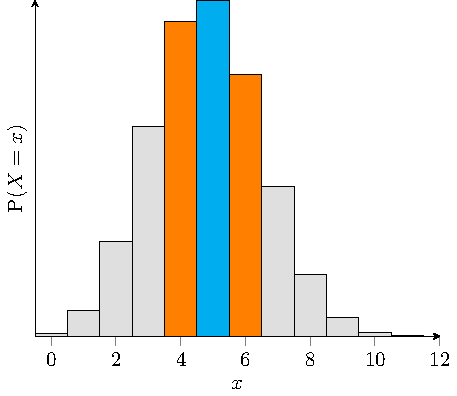
\includegraphics{../Diagrams/Binomial-Distribution/Binomial-Distribution.pdf}
  \caption{\ref{source:binomial-distribution} The histogram for a binomial distribution \(X\sim\operatorname{B}(10,p)\) that has mode \(m=5\).}
  \label{fig:binomial-distribution}
\end{figure}
\begin{example}{2018 TPJC JC2 H2 MYE P2 8}{}
  On average, 3.5\% of a certain brand of chocolate turn out misshapen. The chocolates are sold in packets of 25.
  \begin{enumerate}[label=(\roman*)]
    \item State, in context, two assumptions needed for the number of misshapen chocolates in a packet to be well modelled by a binomial distribution.
    \item Explain why one of the assumptions stated in part (i) may not hold in this context.
  \end{enumerate}
  \textit{Answer:}
  \begin{enumerate}[label=(\roman*)]
    \item 
    \begin{enumerate}[label=\arabic*.]
      \item Each chocolate is \emph{equally likely} (3.) to be misshapen.
      \item The event that a chocolate is misshapen is \emph{independent} (2.) of the event that another chocolate is misshapen.
    \end{enumerate}
    \item While on average, the probability that a chocolate is misshapen is 3.5\%, it is possible that there are more misshapen chocolates at certain times, possible due to equipment malfunction, which would mean the probability is not constant.\\[3mm]
    OR\\[3mm]
    Misshapen chocolates could be the result of equipment used and as the equipment used would not be the same for the same portion of the chocolate produced, whether a chocolate is misshapen may not be independent of another chocolate being misshapen.
  \end{enumerate}
\end{example}
\chapter{Continuous Random Variables}
\begin{stbox}{General Information}
  \begin{itemize}
    \item A function \(f \colon \mathbb{R}\to \mathbb{R}\) is a \emph{probability density function} (pdf) of a continuous random variable \(X\) iff \(f\) is nonnegative and \(\int_{-\infty}^{\infty}f(x)\,dx=1\).
    \item For any probability mass function \(f\), we have \(\Prob(a\leq X\leq b)=\int_{a}^{b}f(x)\,dx\). Whether the inequality is strict or nonstrict does not affect the above identity. 
    \item A \emph{mode} of \(X\) is any value \(m\) such that \(f(m)\) is maximum.
    \item A \emph{cumulative distribution function} (cdf) \(F \colon \mathbb{R}\to [0,1]\) of a random variable \(X\) is defined by
    \[F(x)\coloneq P(X\leq x)=\int_{-\infty}^{x}f(x)\,dx.\]
    \item When writing out the cdf as a piecewise function, we explicitly write out the range of values for each case. We reserve the use of ``otherwise'' for pdf's.
    \item Any cdf is continuous and nondecreasing.
    \item Let \(X\) be a continuous random variable with cdf \(F\). To find the pdf \(g\) of any \(Y(X)\), we first find its cdf, then differentiate. We achieve this by reverse engineering \(Y(X)\leq y\) to find an inequality that relates \(X\) with \(y\). E.g. \(e^X\leq y\) iff \(X\leq \ln(y)\).
    \item A \emph{median} of \(X\) is any value \(m\) such that \(\Prob(X\leq m)=F(m)=1/2\).
    \item Mean/Expectation: 
    \[\mu=\E(X)\coloneq \int_{-\infty}^{\infty}xf(x)\,dx \qquad\text{and}\qquad \E(g(X))=\int_{-\infty}^{\infty}g(x)f(x)\,dx.\]
    \item Important property: 
    \[\E(ag(X)\pm bh(x))=a\E(g(X))\pm\E(h(X)).\]
    \item Variance: 
    \[\Var(X)\coloneq \E(X^2)-[\E(X)]^2.\]
    \item Important property:
    \[\Var(aX\pm b)=a^2\Var(X).\]
  \end{itemize}
\end{stbox}
\chapter{Special Continuous Random Variables}
\begin{definition}{}{}
  A continuous random variable \(X\) has a \emph{normal distribution} with mean \(\mu\) and standard deviation \(\sigma\), denoted by \(X \sim \operatorname{N}(\mu,\sigma^2)\), iff its pdf \(f\) is such that 
  \[f(x)=\frac{1}{\sigma\sqrt{2\pi}}\exp\left(-\frac{(x-\mu)^2}{2\sigma^2}\right).\]
\end{definition}
\begin{stbox}{General Information}
  \begin{itemize}
    \item A normal distribution is symmetrical about the line \(x=\mu\). That is 
    \[\Prob(X\leq\mu-\delta)=\Prob(X\geq\mu+\delta)\]
    for each \(\delta>0\). Note that the mean, median, and mode coincide with \(\mu\).
    \item Properties of the normal distribution. Let \(X\) and \(Y\) be independent, such that \(X \sim \operatorname{N}(\mu,\sigma^2)\) and \(Y \sim \operatorname{N}(m,s^2)\). Then, for any \(n \in \mathbb{N}\) and \(x\), \(y \in \mathbb{R}\),  
    \begin{itemize}
      \item \(nX \sim \operatorname{N}(n\mu,n^2\sigma^2)\),
      \item \(X_1+X_2+\cdots+X_n \sim \operatorname{N}(n\mu,n\sigma^2)\),
      \item \(aX\pm bY \sim \operatorname{N}(a\mu\pm bm,a^2\sigma^2+b^2s^2)\).
    \end{itemize}
    \item At times, the question may be phrased in a misleading manner. Try using some inference to figure out the intended interpretation.
  \end{itemize}
\end{stbox}
\begin{example}{}{}
  ``The mass of the padding is \(30\%\) of the mass of a randomly selected light bulb of mass \(L\). Find the probability that a light bulb with padding has mass \(c\).'' 
    
  Then for any light bulb of mass \(L_1\), the mass of the padding is \(0.3L_2\) (and \emph{not} \(0.3L_1\)). i.e. we are to find \(\Prob(L_1+0.3L_2)\).
\end{example}
\begin{stbox}{}
  \begin{itemize}
    \setcounter{enumi}{3}
    \item A variable \(Z\sim \operatorname{N}(0,1)\) is said to follow the \emph{standard} normal distribution.

    \emph{Note}: \(Z\) is reserved for this purpose.
    \item Let \(X \in \operatorname{N}(\mu,\sigma^2)\). Then, \(\frac{X-\mu}{\sigma}\) follows the standard normal distribution. 
    \item What \texttt{Tail} do we select for \texttt{invNorm}?
    \begin{center}
      \begin{tabular}{|Sc|Sc|}
        \hline
        \(\Prob(X<x)=p\) & \texttt{LEFT}\\
        \hline
        \(\Prob(-x<X<x)=p\) & \texttt{CENTER}\\
        \hline
        \(\Prob(X>x)=p\) & \texttt{RIGHT}\\
        \hline
      \end{tabular}
    \end{center}
    \item When using \texttt{invNorm} on an inequality, what should the sign be? For simplicity, we write \(\mathscr{L}(p)=\texttt{invNorm}(p,0,1,\texttt{RIGHT})\), and \(\mathscr{R}(p)=\texttt{invNorm}(p,0,1,\texttt{LEFT})\). Then,
    \begin{center}
      \begin{tabular}{|Sc|Sc|Sc|}
        \hline
        \(\Prob(Z>z)\geq p\) & \(z\leq \mathscr{L}(p)\)\\
        \hline
        \(\Prob(Z>z)\leq p\) & \(z\geq \mathscr{L}(p)\)\\
        \hline
        \(\Prob(Z<z)\geq p\) & \(z\geq \mathscr{R}(p)\)\\
        \hline
        \(\Prob(Z<z)\leq p\) & \(z\leq \mathscr{R}(p)\)\\
        \hline
      \end{tabular}
    \end{center}
  \end{itemize}
\end{stbox}
\begin{example}{}{}
  Suppose we want to find the least integer value of \(m\) for which \(\Prob(Z>1-m)\geq 1/2\).

  Then, using \texttt{invNorm (RIGHT)}, we infer that \(z\leq 0\), \emph{not} \(z\geq 0\). An illustration: 
  \begin{figure}[H]
    \centering
    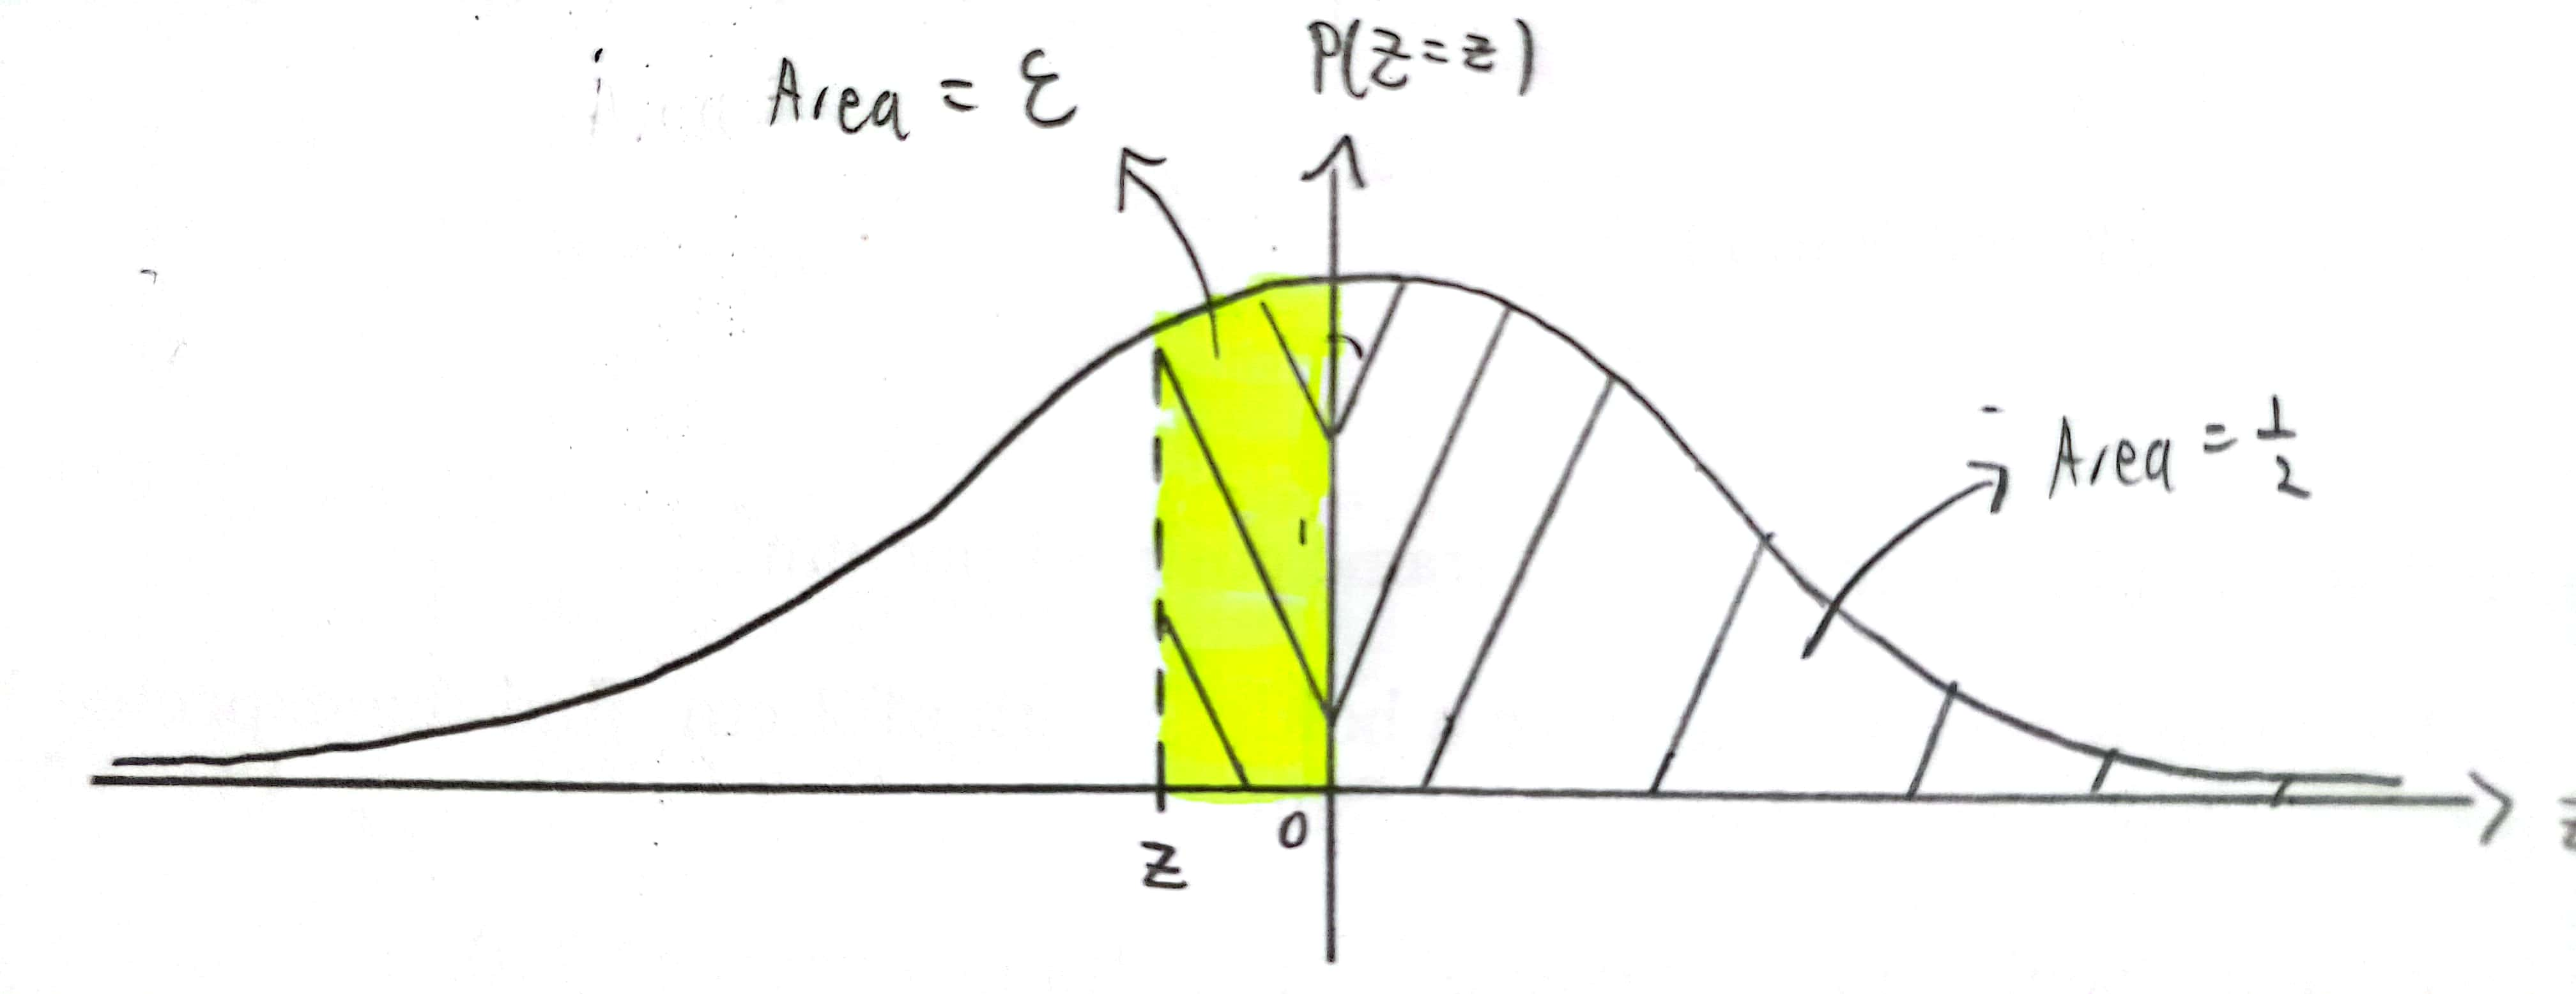
\includegraphics[width=\textwidth]{../images/Special-Continuous-Random-Variables-Example-Illustration.jpg}
    \caption{\ref{Me} Illustration of the inverse norm function.}
    \label{fig:inverse-norm}
  \end{figure}
\end{example}
\begin{definition}{}{}
  A continuous random variable \(X\) has a \emph{uniform distribution} over the interval \((a,b)\), which is denoted by \(X \sim \operatorname{U}(a,b)\), iff its pdf \(f\) is such that
    \[f(x)=\begin{cases}
      \frac{1}{b-a} &\text{if \(a<x<b\),}\\
      0 &\text{otherwise.}
    \end{cases}\] 
\end{definition}
\begin{note}
  Let \(l\) and \(u\) be the lower and upper quartiles, of a normal distribution \(X\sim\Normal(\mu,\sigma^2)\). i.e. \(\Prob(X<l)=1/4\) and \(\Prob(X<u)=3/4\). Then, 
  \[\Prob{\left( \mu-\highlight[yellow]{\frac{u-l}{2}}<X<\mu+\highlight[yellow]{\frac{u-l}{2}} \right)}=\Prob(l<X<u)=1/2.\]
\end{note}
\begin{definition}{}{}
  A continuous random variable \(Y\) has an (negative) exponential distribution, which we denote with \(Y\sim \operatorname{Exp}(\lambda)\), iff its pdf \(g\) is such that
    \[g(x)=
    \begin{cases}
      \lambda e^{-\lambda x} &\text{if \(x\geq 0\)},\\
      0 &\text{otherwise.}
    \end{cases}\]
  (An exponential distribution models time between occurrences.)
\end{definition}
\begin{note}
  The memorylessness of the exponential distribution. Let \(Y \sim \operatorname{Exp}(\lambda)\), then
  \[\Prob(Y>z+y \,\vert\, Y>y)=\Prob(Y>z) \qquad\text{and}\qquad\Prob(Y<z+y \,\vert\, Y>y)=\Prob(Y<z).\]
  % In general, it also holds that 
  % \[\Prob(V>z+y \,\vert\, V>y)=1-\Prob(V<z+y \,\vert\, V>y)\]
  % for any random variable \(V\).
\end{note}
\begin{stbox}{}
  \begin{itemize}
    \item Expectation and variance:
    \begin{center}
      \begin{tabular}{|Sc|Sc|Sc|}
        \hline
        Distribution & Expectation & Variance\\
        \hline
        \(X\sim \operatorname{U}(a,b)\) & \(\dfrac{a+b}{2}\) & \(\dfrac{(b-a)^2}{12}\)\\
        \hline
        \(Y\sim \operatorname{Exp}(\lambda)\) & \(\dfrac{1}{\lambda}\) & \(\dfrac{1}{\lambda^2}\)\\
        \hline
      \end{tabular} 
    \end{center}
    \emph{Note}: We need to remember the expectation and variance for the uniform distribution, as it is not provided in the MF26 formula sheet (unlike all other distributions).
    \item \emph{Warning}: The G.C. tends to incorrectly process an integral if its upper and lower bounds contain \(\pm \text{E}99\).
    \item Let \(T\) be the time taken between two consecutive arrivals and \(\#\sim\operatorname{Po}(\lambda t)\) the number of arrivals in time \(t\). Then, 
    \[\Prob(T>t)=\Prob(\#=0)=e^{-\lambda t}.\]
    As such, the probability that there is at least one arrival in an interval of time \(t\) is 
    \[\Prob(T\leq t)=1-e^{-\lambda t}.\]  
  \end{itemize}
\end{stbox}
\begin{note}
  The exponential distribution \emph{begins from zero}. But, contextually, we may begin counting from \emph{one}! Hence, we need to be careful of what bounds to use in probability calculations.   
\end{note}
\begin{example}{}{}
  Find the probability \(p\) that the company received the first response in the third hour of the day. (It is implied the that there's no zeroth hour.)
  
  \vspace{-0.5\baselineskip}\rule{20cm-137.0549pt}{0.05mm}

  Let \(T\sim\Exp(\lambda)\). Then, \(p=\Prob(2\leq T<3)\neq\Prob(3\leq T<4)\).
  \begin{figure}[H]
    \centering
    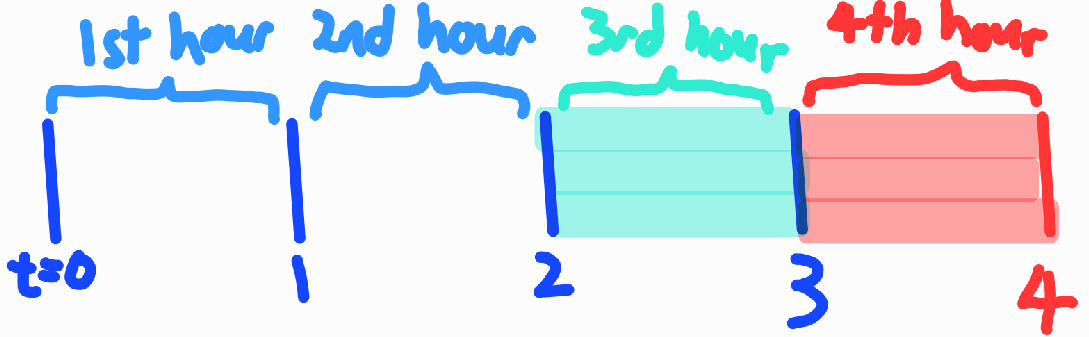
\includegraphics[width=0.5\textwidth]{../Diagrams/exp-example.pdf}
    \caption{\ref{Me}}
    \label{fig:exp-bounds-note-example}
  \end{figure}
\end{example}
\chapter{Sampling and Estimation}
\begin{definition}{}{}
  A sample is a finite subset of the population.
\end{definition}
\begin{definition}{}{}
  A random sample is a sample selected such that each member of the population has an equal probability of being selected into the sample.
\end{definition}
\begin{note}
  State, in context, what it means for the sample to be random.
  \begin{center}
    \parbox{0.9\textwidth}{
      It means that \hly{every [a member of the population]} has \hly{an equal probability} of being \hly{selected into the sample}. 
    }
  \end{center}
\end{note}
\begin{note}
  Explain why the sample would actually not be random.
  \begin{center}
    \parbox{0.9\textwidth}{
      [Contextual reason], so \hly{not all} the [members of the population] have an \hly{equal probability of being selected into the sample}. 
    }
  \end{center}
\end{note}
\begin{definition}{}{}
  Any statistic \(T\) derived from a random sample and used to estimated an unknown population parameter \(\theta\) is known as an \emph{estimator}. It is an \emph{unbiased} estimator iff \(\E(T)=\theta\). If \(T\) is unbiased we commonly write \(\hat{\theta}\) for \(T\).
\end{definition}
\begin{stbox}{General Information}
  \begin{itemize}
    \item Either write \(\hat{\mu}\highlight[yellow]{=\bar{x}}=\dots\) or write out ``Unbiased estimate of the population mean \(\mu\), \(\widebar{x}=\dots\)'' Same holds for other population parameters \(\theta\).
    \item Estimators you should know:
    \item 
    % *A table where Parameter is under another column
    % \begin{center}
    %   \begin{tabular}{|Sc|Sc|Sc|Sc|Sc|}
    %     \hline
    %     \multicolumn{2}{|Sc|}{Parameter} & Estimator & Unbiased? & Formula\\
    %     \hline
    %     Population Mean & \(\mu\) & \(\widebar{X}\) & \checkmark & \(\dfrac{X_1+X_2+\dots+X_n}{n}\)\\
    %     \hline
    %     \multirow{2}{*}[-1.2cm]{Population Variance} & \multirow{2}{*}[-1.2cm]{\(\sigma^2\)} & \(\sigma_n^2\) & \(\times\) & 
    %     \begin{minipage}{3cm}
    %       \begin{center}
    %         \(\dfrac{\sum{(X_i-\widebar{X})^2}}{n}\)\\[1mm]
    %         \(\dfrac{\sum{X_i^2}}{n}-\widebar{X}^2\)
    %       \end{center}
    %     \end{minipage}\\
    %     \cline{3-4}
    %     & & \(S^2\) & \checkmark & 
    %     \begin{minipage}{5cm}
    %       \begin{center}
    %       \(\dfrac{n}{n-1}\sigma_n^2\)\\[1mm]
    %       \(\dfrac{\sum(X_i-\widebar{X})^2}{n-1}\)\\[1mm]
    %       \(\dfrac{1}{n-1}\left[ \sum X_i^2-\dfrac{(\sum X_i)^2}{n} \right]\)
    %       \end{center}
    %     \end{minipage}\\
    %     \hline
    %     Population Proportion & \(p\) & \(P_s\) & \checkmark & \(\dfrac{X}{n}\)\\
    %     \hline
    %   \end{tabular}
    % \end{center}
    \begin{center}
      \resizebox{0.94\textwidth}{!}{\begin{tabular}{|Sc|Sc|Sc|Sc|}
        \hline
        Parameter & Estimator & Unbiased? & Formula(s)\\
        \hline
        Population Mean \(\mu\) & Sample Mean \(\widebar{X}\) & \checkmark & \(\dfrac{X_1+X_2+\dots+X_n}{n}\)\\
        \hline
        \multirow{2}{*}[-1.2cm]{Population Variance \(\sigma^2\)} & Sample Variance \(\sigma_n^2\) & \(\times\) & 
        \begin{minipage}{3cm}
          \begin{center}
            \(\dfrac{\sum{(X_i-\widebar{X})^2}}{n}\)\\[1mm]
            \(\dfrac{\sum{X_i^2}}{n}-\widebar{X}^2\)
          \end{center}
        \end{minipage}\\
        \cline{2-4}
        & \(S^2\) & \checkmark & 
        \begin{minipage}{5cm}
          \begin{center}
          \(\dfrac{n}{n-1}\sigma_n^2\)\\[1mm]
          \(\dfrac{\sum(X_i-\widebar{X})^2}{n-1}\)\\[1mm]
          \(\dfrac{1}{n-1}\left[ \sum X_i^2-\dfrac{(\sum X_i)^2}{n} \right]\)
          \end{center}
        \end{minipage}\\
        \hline
        Population Proportion \(p\) & Sample Proportion \(P_s\) & \checkmark & \(\dfrac{X}{n}\)\\
        \hline
      \end{tabular}}
    \end{center}
    \item Let \(X\) be a random variable following \emph{any distribution}, and suppose we have a random sample \(X_1,X_2,\dots,X_n\) of size \(n\geq 50\). Then by CLT (Central Limit Theorem), since \(n\geq 50\) is large, 
    \[\widebar{X}\sim \Normal\left(\mu,\frac{\sigma^2}{n}\right) \qquad\text{and}\qquad X_1+X_2+\dots+X_n\sim \Normal(n\mu,n\sigma^2)\]
    \emph{approximately}.
    \item Assumptions when using CLT:
    \begin{itemize}
      \item The sample is random.
      \item Each \(X_i\) is independent and identically distributed.
    \end{itemize}
    \item Suppose \(X\sim \Normal(\mu,\sigma^2)\) is known and we pick a \emph{particular} sample. Then,
    \begin{center}
      \begin{tabular}{|Sc|Sc|Sc|}
        \hline
        Distribution & Is An Approximation?\\
        \hline
        \(\widebar{X} \sim \Normal(\mu,\sigma^2)\) & No\\
        \hline
        \(\widebar{X} \sim \Normal(\widebar{x},\sigma^2)\) & Yes\\
        \hline
        \(\widebar{X} \sim \Normal(\mu,s^2)\) & Yes\\
        \hline
        \(\widebar{X} \sim \Normal(\widebar{x},s^2)\) & Yes\\
        \hline
      \end{tabular}
    \end{center}
    % ADD NAMES of the parameters and estimators to previous table
    So, if we obtain any of the latter three in solving a question, we must write ``\(X\sim \Normal(\rule{3mm}{0.1mm},\rule{3mm}{0.1mm})\) approximately'' (even though we knew \(X\) \emph{exactly} follows a normal distribution!)
    \item Pooled estimators. First assume we have two populations, from which we select a random sample of size \(n_1\) and \(n_2\). We let \(\widebar{X}_1\) and \(S_1^2\) denote the sample mean and unbiased estimator for variance, respectively, for the first sample. Similarly define \(\widebar{X}_2\) and \(S_2^2\), for the second sample.
    \begin{center}
      \begin{tabular}{|Sc|Sc|}
        \hline
        Parameter & Unbiased Pooled Estimator\\
        \hline
         Mean  & \(\hat{\mu}=\dfrac{n_1\widebar{X}_1+n_2\widebar{X}_2}{n_1+n_2}\)\\
         \hline
         Variance & \(S_p^2=\dfrac{(n_1-1)S_1^2+(n_2-1)S_2^2}{n_1+n_2-2}\)\\
         \hline
      \end{tabular}
    \end{center}
  \end{itemize}
\end{stbox}
The following definition is found in 
\href{https://www.amazon.com/Introduction-Mathematical-Statistics-8th-Whats-dp-0134686993/dp/0134686993/ref=dp_ob_title_bk}{Hogg-McKean-Craig}. Similar definitions are also found in 
\href{https://www.amazon.sg/Mathematical-Statistics-Applications-William-Mendenhall/dp/0495110817#customerReviews}{Wackerly-Mendenhall-Schaefer}
and \href{https://www.amazon.com/Probability-Statistical-Inference-Statistics-Monographs/dp/0824703790}{Nitis Mukhopadhyay}.
\begin{definition}{}{}
  Let \(X_1,X_2,\dots,X_n\) be a sample on a random variable \(X\), where \(X\) has pdf \(f(x;\theta)\), \(\theta \in \Omega\). Let \(0<\alpha<1\) be specified. Let \(L=L(X_1,X_2,\dots,X_n)\) and \(U=U(X_1,X_2,\dots,X_n)\) be two statistics. We say that the interval \((L,U)\) is a \((1-\alpha)100\%\) \emph{confidence interval} for \(\theta\) iff 
  \[1-\alpha=P_\theta[\theta \in (L,U)].\]
  That is, the probability that the interval contains \(\theta\) is \(1-\alpha\), which is called the \emph{confidence coefficient} or \emph{confidence level} of the interval.
\end{definition}
\begin{stbox}{}
  \begin{itemize}
    \item We cannot write ``a \(1-\alpha\) (e.g. 0.95) confidence interval''. The \(1-\alpha\) must always be expressed as a \emph{percentage}.
    % \item Let \(0<\alpha<1\) and \(X_1,X_2,\dots,X_n\) be a sample on a random variable \(X\). Suppose \(n\) is large (\(n\geq 50\)). Then, CLT allows us to obtain the approximation
    % \[\frac{\widebar{X}-\mu}{\frac{S}{\sqrt{n}}}=Z\sim \Normal(0,1).\]
    % Rewriting \(\Prob(-z_{1-\alpha/2}<Z<z_{1-\alpha/2})=1-\alpha\) gives
    % \[\Prob\left( \widebar{x}-z_{1-\alpha/2}\frac{s}{\sqrt{n}}<\mu<\widebar{x}+z_{1-\alpha/2}\frac{s}{\sqrt{n}}\right)=1-\alpha.\] 
    % As such, a \((1-\alpha)100\%\) confidence interval is
    % \[\left( \widebar{x}-z_{1-\alpha/2}\frac{s}{\sqrt{n}}\,,\ \widebar{x}+z_{1-\alpha/2}\frac{s}{\sqrt{n}} \right).\]
    % When the variance \(\sigma^2\) is known, we can replace \(s\) with \(\sigma\).
    \item Let \(\hat{\theta}\) be a statistic that is normally distributed with mean \(\theta\) and standard error \(\sigma_{\hat{\theta}}\). We see that 
    \[\frac{\hat{\theta}-\theta}{\sigma_{\hat{\theta}}}=Z \sim \Normal(0,1).\]
    Rewriting \(\Prob(-z_{1-\alpha/2}<Z<z_{1-\alpha/2})=1-\alpha\) gives
    \[\Prob(\hat{\theta}-z_{1-\alpha/2}\sigma_{\hat{\theta}}<\theta<\hat{\theta}+z_{1-\alpha/2}\sigma_{\hat{\theta}})=1-\alpha.\]
    Hence, a \((1-\alpha)100\%\) confidence interval for \(\theta\) is
    \[(\hat{\theta}-z_{1-\alpha/2}\sigma_{\hat{\theta}}\,,\ \hat{\theta}+z_{1-\alpha/2}\sigma_{\hat{\theta}}).\]
    \href{https://www.amazon.sg/Mathematical-Statistics-Applications-William-Mendenhall/dp/0495110817#customerReviews}{(Wackerly-Mendenhall-Schaefer)}
    \item Let \(0<\alpha<1\) and \(X_1,X_2,\dots,X_n\) be a sample on a random variable \(X\) with population mean \(\mu\), where \(n\) is large. Then, an approximate \((1-\alpha)100\%\) confidence interval for \(\mu\) is
    \[\left( \widebar{x}-z_{1-\alpha/2}\frac{s}{\sqrt{n}}\,,\ \widebar{x}+z_{1-\alpha/2}\frac{s}{\sqrt{n}} \right).\]
    When the population variance \(\sigma^2\) is known, we can replace \(s\) with \(\sigma\). If the distribution of \(X\) is known to be normal, in addition to \(\sigma^2\) being known exactly, then the confidence interval is exact; it is not just an approximation. 

    \href{https://www.amazon.com/Introduction-Mathematical-Statistics-8th-Whats-dp-0134686993/dp/0134686993/ref=dp_ob_title_bk}{(Hogg-McKean-Craig)}
    \item Let \(X\) be a Bernoulli random variable with probability of success \(p\), where \(X\) is 1 or 0 if the outcome is success or failure, respectively. Suppose \(X_1,X_2,\dots,X_n\) is a random sample from the distribution of \(X\), where \(n\) is large. Let \(\hat{p}=\widebar{X}\) be the sample proportion of successes. Then, an approximate \((1-\alpha)100\%\) confidence interval for \(p\) is given by 
    \[\left( \hat{p}-z_{1-\alpha/2}\sqrt{\frac{\hat{p}(1-\hat{p})}{n}}\,,\ \hat{p}+z_{1-\alpha/2}\sqrt{\frac{\hat{p}(1-\hat{p})}{n}} \right).\]
    (Letting \(Y=X_1+X_2+\dots+X_n\sim \operatorname{B}(n,p)\) gives \(\hat{p}=Y/n\), which is the presentation used in the school's notes.) 

    \href{https://www.amazon.com/Introduction-Mathematical-Statistics-8th-Whats-dp-0134686993/dp/0134686993/ref=dp_ob_title_bk}{(Hogg-McKean-Craig)}
  \end{itemize}
\end{stbox}
\begin{note}
  Standard phrasing for the interpretation of a \((1-\alpha)100\%\) confidence interval \((a,b)\). 
  \begin{center}
    \parbox{0.9\textwidth}{
      The probability that the interval \((a,b)\) contains the true value of the [population mean/proportion in context] is \(1-\alpha\).
    }
  \end{center}
\end{note}
\begin{note}
  Standard phrasing for what is a \((1-\alpha)100\%\) confidence interval for \(\theta\)?
  \begin{center}
    It is an interval which has probability \(1-\alpha\) of containing the true value of \(\theta\).  
  \end{center}
\end{note}
\begin{note}
  Standard phrasing for whether mean/proportion in context has likely increased/decreased, when given suitable confidence intervals.
  \begin{enumerate}
    \item There is no conclusive result.

    Since the old and new \((1-\alpha)\%\) confidence intervals overlap, we are unable to conclude whether the [mean/proportion in context] has decreased or not. Hence, it is inconclusive from these figures as to whether the [context (e.g. an awareness campaign)] has been effective.
    \item It has likely increased/decreased.
    
    The old \((1-\alpha)\%\) confidence interval is to the left/right of the new \((1-\alpha)\%\) confidence interval, such that they do not overlap. So, can conclude that the [mean/proportion in context] likely increased/decreased. Hence, these figures suggests that the [context (e.g. an awareness campaign)] has been effective.
  \end{enumerate}
\end{note}
\begin{note}
  Advantage and disadvantage of a \((1-\beta)\%\) confidence interval compared to a \((1-\alpha)\%\) confidence interval, where \(\beta<\alpha\).
  \begin{center}
    \begin{tabular}{ll}
      Advantage:& A \((1-\beta)\%\) CI is more likely to contain the true mean.\\
      Disadvantage:& A \((1-\beta)\%\) CI is less precise (or wider).
    \end{tabular}
  \end{center}
  \emph{Note.} Clearly state which is the advantage and disadvantage, as illustrated above.
\end{note}
\begin{GCSkills}{}
  Calculating statistics (i.e. \(\widebar{x}\), \(s\), etc) by G.C. given data for a sample.
  \begin{enumerate}
    \item Keying in the data: \texttt{stat} \(\Longrightarrow\) \texttt{1:Edit} \(\Longrightarrow\) Key in the data into one of the lists \(\texttt{L}_i\). 
    \item Calculating the statistic: \texttt{stat} \(\Longrightarrow\) \texttt{CALC} \(\Longrightarrow\) \texttt{1-Var Stats} (\texttt{List:}\(\texttt{L}_i\)) \(\Longrightarrow\) \texttt{Calculate}.
    \item Getting the statistic for further calculations: \texttt{vars} \(\Longrightarrow\) \texttt{5:Statistics} \(\Longrightarrow\) Select the desired statistic.
  \end{enumerate}
\end{GCSkills}
\begin{GCSkills}{}
  Calculating the symmetric confidence interval for a normally distributed random variable.
  \begin{center}
  \begin{tabular}{ll}
    Mean: & \texttt{stat} \(\Longrightarrow\) \texttt{TESTS} \(\Longrightarrow\) \texttt{7:ZInterval\dots}\\
    Proportion: & \texttt{stat} \(\Longrightarrow\)\texttt{TESTS} \(\Longrightarrow\) \texttt{A:1-PropZInt\dots}\\ 
  \end{tabular}
  \end{center}
\end{GCSkills}
\begin{titlednote}{combining two samples into one.}
  Let \(X\) be a random variable with population mean \(\mu\). We are given two independent random samples \(A\) and \(B\), of sizes \(m\) and \(n\), respectively. Find a \(100(1-\alpha)\%\) confidence interval for \(\mu\), based on the combined sample \(C\). 
  \begin{align*}
    \widebar{x}_C&=\frac{\sum{x_A}+\sum{x_B}}{m+n}=\frac{m\widebar{x}_A+n\widebar{x}_B}{m+n}\\
    s_C^2&=\highlight[green!50]{\frac{1}{m+n-1}\left( \sum{x_A^2}+\sum{x_B^2}-\frac{(\sum{x_A}+\sum{x_B})^2}{m+n} \right)}\neq\highlight[red!30]{\frac{(m-1)s_A^2+(n-1)s_B^2}{m+n-2}}.
  \end{align*}
  Proceed with the usual calculations to find the \(100(1-\alpha)\%\) confidence interval based on \(C\).
\end{titlednote}
\chapter{Statistics: Hypothesis Testing}
\section{Preliminary Definitions}
\begin{definition}{}{}
  The \emph{null hypothesis} \(H_0\) and \emph{alternative hypothesis} \(H_1\) are the hypotheses that we hope to reject and accept, respectively. 
\end{definition}
\begin{note}
  To check we have correctly stated the hypotheses in our hypothesis test, ensure that they are contrasting. For example, we are testing A's claim that \(\mu>\mu_0\):

  \begin{minipage}{0.45\textwidth}
    \vspace{\baselineskip}
    \begin{tabular}{|ll|}
      \hline
      Test & \(H_0\colon\mu=\mu_0\) (A's claim is false)\\
      against &\(H_1\colon\mu<\mu_0\) (A's claim is false)\\
      \multicolumn{2}{|l|}{at the \(100\alpha\%\) significance level.}\\
      \hline
    \end{tabular}

    \vspace{\baselineskip}
    Both hypotheses result in A's claim being false. Hence, the hypotheses have been stated erroneously \textcolor{red}{\(\times\)}.  
  \end{minipage}%
  \hfill
  \begin{minipage}{0.45\textwidth}
    \vspace{\baselineskip}
    \begin{tabular}{|ll|}
      \hline
      Test & \(H_0\colon\mu=\mu_0\) (A's claim is false)\\
      against &\(H_1\colon\mu>\mu_0\) (A's claim is true)\\
      \multicolumn{2}{|l|}{at the \(100\alpha\%\) significance level.}\\
      \hline 
    \end{tabular}  

    \vspace{\baselineskip}
    The hypotheses are contrasting. So, they have been correctly stated \textcolor{green!70!black}{\checkmark}. 
    \vspace{\baselineskip}
  \end{minipage}
\end{note}
\begin{stbox}{General Information}
  \begin{itemize}
    \item Without going into details, a \emph{critical region} \(C\) is just a set that defines the decision rule / test 
    \begin{center}
      Reject \(H_0\) (Accept \(H_1\)) \quad if \((X_1,X_2,\dots,X_n)\in C\),
    \end{center}
    for any random sample \(X_1,X_2,\dots,X_n\) from the distribution of a random variable \(X\).
  \end{itemize}
\end{stbox}
\begin{definition}{}{}
  The \emph{significance level} \(100\alpha\%\) of a test is the probability of rejecting \(H_0\) when it is in fact true. i.e. \(\alpha=\Prob(H_0\text{ is rejected}\,\vert\,H_0\text{ is true})\).
\end{definition}
\begin{note}
  Explain, in context, the meaning of `at the \(\alpha\%\) level of significance'.
  \begin{center}
    \parbox{0.9\textwidth}{
      The probability that we conclude [\(H_1\) in context], when actually [\(H_0\) in context], is \(\alpha\%\).
    }
  \end{center}
\end{note}
\begin{definition}{}{}
  The \emph{\(p\)-value} is the lowest level of significance for which the null hypothesis will be rejected. In other words, for the null hypotheses
    \begin{center}
      \begin{enumerate*}[label=(\alph*),itemjoin={\quad}]
        \item \(\mu<\mu_0\),
        \item \(\mu \neq \mu_0\),
        \item \(\mu>\mu_0\),
      \end{enumerate*}
    \end{center}
    we have
    \begin{center}
      \begin{enumerate*}[label=(\alph*),itemjoin={\quad}]
        \item \(p\text{-value}\coloneq\Prob(Z\leq z_\text{calc})\),
        \item \(p\text{-value}\coloneq\Prob(\lvert Z \rvert\geq \lvert z_\text{calc} \rvert)\),
        \item \(p\text{-value}\coloneq\Prob(Z\geq z_\text{calc})\).
      \end{enumerate*}
    \end{center}
\end{definition}
\begin{note}
  Explain what the \(p\)-value means in context.
  \begin{center}
    \parbox{0.9\textwidth}{
      The \(p\)-value is the least level of significance to conclude that [\(H_1\) in context].
    }
  \end{center}
\end{note}
\section{One Sample \(z\)-Test}
\begin{stbox}{General Information}
  There are various combinations of assumptions for which this test applies, and two variants of the corresponding test statistic. For brevity, we shall avoid restating it, instead directing the reader to table \ref{Table:Summary table for one-sample hypothesis testing.}.
    \begin{enumerate}
      \item Let [\(X\) in context] and \(\mu\) be its population mean.
      \item 
      \begin{tabular}{|ll|}
        \hline
        Test & \(H_0\colon\mu=\mu_0\)\\
        against &\(H_1\colon\) 
        \begin{enumerate*}[itemjoin={\quad}]
          \item \(\mu<\mu_0\),
          \item \(\mu \neq \mu_0\),\quad or
          \item \(\mu>\mu_0\),
        \end{enumerate*}\\
        \multicolumn{2}{|l|}{at the \(100\alpha\%\) significance level.}\\
        \hline
      \end{tabular}
      \item Under \(H_0\), since the sample size \(n=\rule{0.5cm}{0.01mm}\) (\(\geq 50\)), by CLT we have \(\widebar{X}\sim \Normal(\mu_0,s^2/n)\) approximately.
      \item Test statistic: 
      \[Z=\frac{\widebar{X}-\mu_0}{s/\sqrt{n}}\sim\Normal(0,1)\qquad\text{approximately},\]
      where \(\widebar{x}=\rule{0.5cm}{0.01mm}\) and \(s=\rule{0.5cm}{0.01mm}\).
    \end{enumerate}
      \begin{minipage}[t]{0.45\textwidth}
        \begin{itemize}
          \item Find \(z_{1-\alpha}\) or \(z_{1-\alpha/2}\), which satisfies
          \begin{enumerate}
            \item \(\Prob(Z<z_\alpha)=\alpha\), 
            \item \(\Prob(-z_{1-\alpha/2}<Z<z_{1-\alpha/2})=1-\alpha\), or
            \item \(\Prob(Z>z_{1-\alpha})=\alpha\).
          \end{enumerate}
          \item Find the test statistic value 
          \[z_\text{calc}=\frac{\widebar{x}-\mu_0}{s/\sqrt{n}}.\]
          \item Reject \(H_0\) iff 
          \begin{enumerate}
            \item \(z_\text{calc}<z_\alpha\),
            \item \(\lvert z_\text{calc} \rvert>z_{1-\alpha/2}\), or
            \item \(z_\text{calc}>z_{1-\alpha}\).
          \end{enumerate}
        \end{itemize}
      \end{minipage}
      \begin{minipage}[t]{0.45\textwidth}
        \begin{itemize}
          \item Find the \(p\)-value using GC.
          \item Reject \(H_0\) iff \(p\)-value is less than \(\alpha\).
        \end{itemize}
        \vfill
        \begin{flushright}
          \begin{minipage}{0.8\textwidth}
            \begin{GCSkills}{}
              Calculating the \(p\)-value of a sample.
              \begin{center}
                \texttt{stat \(\Longrightarrow\) TESTS \(\Longrightarrow\) 1:Z-Test\dots}
              \end{center}
            \end{GCSkills}
          \end{minipage}
        \end{flushright}
      \end{minipage}
      \begin{enumerate}
        \item[5.] Since\quad
        \begin{enumerate*}[label=(\alph*),itemjoin={\quad}]
          \item \(z_\text{calc}<z_\alpha\),
          \item \(\lvert z_\text{calc} \rvert>z_{1-\alpha/2}\),
          \item \(z_\text{calc}>z_{1-\alpha}\),\quad or\quad \(p\text{-value}<\alpha\),
        \end{enumerate*}
        we reject \(H_0\). There is sufficient evidence at the significance level \(100\alpha\%\) that [\(H_1\) in context].
      \end{enumerate}
\end{stbox}
\begin{note}
  If we have a null hypothesis, such as
      \begin{center}
        \(H_0\colon\mu\leq\mu_0\)\quad or\quad \(H_0\colon\mu\geq\mu_0\),
      \end{center}
      we can just use \(H_0\colon\mu=\mu_0\) instead.
\end{note}
% \begin{definition}{}{}
%   We say a critical region \(C\) is of \emph{size} \(\alpha\) if 
%   \[\alpha=\max_{\theta\in\omega_0}P_\theta[(X_1,X_2,\dots,X_n)\in C].\]
%   In our syllabus, \(\alpha\cdot100\%\) is called the \emph{significance level}.
% \end{definition}
\begin{note}
  Explain why there is no need to assume that the distribution of \(X\) is normal/know anything about the population distribution of \(X\).
  \begin{center}
    \parbox{0.9\textwidth}{
      As the \hly{sample size \(n\) is large}, by the \hly{Central Limit Theorem}, the \hly{sample mean} of [random variable \(X\) in context] will \hly{approximately follow a normal distribution}.
    }
  \end{center}
  \emph{Note.} Spell ``Central Limit Theorem'' and ``the sample mean'' out \emph{in full}. Do not use CLT or \(\widebar{X}\) for this question.
\end{note}
\begin{note}
  Explain why a two-tail test should be used instead of a one-tail test. 
  \begin{center}
    \parbox{0.9\textwidth}{We want to see if [\(\mu_X\) in context] has changed, which could be greater than or less than the original population mean time.}
  \end{center}
\end{note}
\section{Student's \(t\)-Distribution}
\begin{definition}{}{}
  A random variable \(X\) follows Student's \(t\)-distribution with \(\nu\) degrees of freedom iff its pdf is
  \[f(t)=\frac{\Gamma{\left( \frac{\nu+1}{2} \right)}}{\sqrt{\pi\nu}\ \Gamma{\left( \frac{\nu}{2} \right)}}\left( 1+\frac{t^2}{\nu} \right)^{-\frac{1}{2}(\nu-1)}.\]
  This is denoted by \(X\sim t(\nu)\).
\end{definition}
\begin{figure}[H]
  \centering
  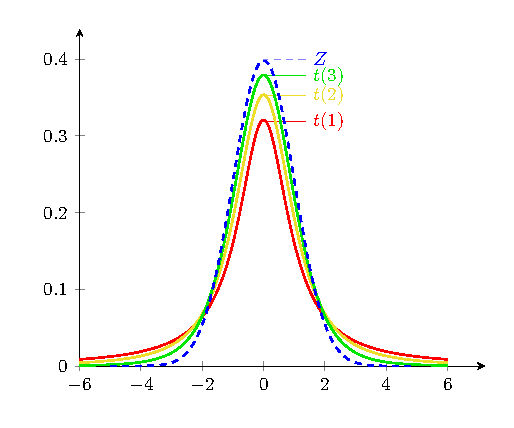
\includegraphics[width=0.5\textwidth]{../Diagrams/t-distribution/t-distributon.pdf}
  \caption{Student's \(t\)-distribution compared to the standard normal distribution.}
  \label{Fig:Student}
\end{figure}
\begin{stbox}{General Information}
  \begin{itemize}
    \item Properties of Student's \(t\)-distribution.
    \begin{enumerate}
      \item It is continuous and symmetric about the vertical axis, i.e. \(t=0\).
      \item From Figure \ref{Fig:Student}, we see that the \(t\)-distribution has a flatter peak and fatter tails, than the standard normal distribution.
      \item As \(\nu\to\infty\), we have \(t(\nu)\to\Normal(0,1)\).
    \end{enumerate}
    \item Let \(T\sim t(n-1)\) and \(t_{(n-1,1-\alpha/2)}\) be such that \(\Prob{\left(-t_{(n-1,1-\alpha/2)}<T<t_{(n-1,1-\alpha/2)}\right)}=1-\alpha\). A \((1-\alpha)100\%\) confidence interval, for the population mean \(\mu\) of \(T\), is
    \[\left( \widebar{x}-t_{(n-1,1-\alpha/2)}\frac{s}{\sqrt{n}}\,,\ \widebar{x}-t_{(n-1,1-\alpha/2)}\frac{s}{\sqrt{n}} \right).\]
    \item Suppose we are conducting the following test:
    \begin{center}
      \begin{tabular}{|ll|}
        \hline
        Test & \(H_0\colon\mu=\mu_0\)\\
        against &\(H_1\colon\mu\neq\mu_0\)\\
        \multicolumn{2}{|l|}{at a \(100\alpha\%\) significance level.}\\
        \hline
      \end{tabular}
    \end{center}
    Then, we reject \(H_0\) iff the appropriate symmetric interval (\(z\) or \(t\)-interval) does \emph{not} contain \(\mu_0\). 
  \end{itemize}
\end{stbox}
\begin{GCSkills}{}
  Calculating the symmetric \(t\)-confidence interval, for the population mean, of a random variable following Student's \(t\)-distribution.
  \begin{center}
    \texttt{stat} \(\Longrightarrow\) \texttt{TESTS} \(\Longrightarrow\) \texttt{8:TInterval\dots} 
  \end{center}
\end{GCSkills}
\section{One Sample \(t\)-Test}
\begin{stbox}{General Information}
    Again, see table \ref{Table:Summary table for one-sample hypothesis testing.} for the necessary assumptions.
    \begin{enumerate}
      \item Let [\(X\) in context] and \(\mu\) be its population mean.
      \item 
      \begin{tabular}{|ll|}
        \hline
        Test & \(H_0\colon\mu=\mu_0\)\\
        against &\(H_1\colon\) 
        \begin{enumerate*}[itemjoin={\quad}]
          \item \(\mu<\mu_0\),
          \item \(\mu \neq \mu_0\),\quad or
          \item \(\mu>\mu_0\),
        \end{enumerate*}\\
        \multicolumn{2}{|l|}{at the \(100\alpha\%\) significance level.}\\
        \hline
      \end{tabular}
      \item Under \(H_0\), the test statistic
      \[T=\frac{\widebar{X}-\mu}{s/\sqrt{n}}\sim t(n-1),\]
      where \(\widebar{x}=\rule{0.5cm}{0.01mm}\) and \(s=\rule{0.5cm}{0.01mm}\).
      \item Continue as per usual, calculating the critical region or the \(p\)-value.
    \end{enumerate}
\end{stbox}
\begin{GCSkills}{}
  Calculating, for a one sample \(t\)-test, the 
  \begin{center}
    \begin{tabular}{ll}
      \(p\)-value: & \texttt{stat} \(\Longrightarrow\) \texttt{TESTS} \(\Longrightarrow\) \texttt{2:T-Test\dots}\\
      critical region: & \texttt{2nd} \(\Longrightarrow\) \texttt{vars} \(\Longrightarrow\) \texttt{4:invT(}
    \end{tabular}
  \end{center}
\end{GCSkills}
\begin{note}
  In the GC, \texttt{invT} is always `to the \texttt{LEFT}'. That is, the output \(t\) of 
  \begin{center}
    \rowcolors{1}{white}{white}
    \begin{tabular}{|lScr|}
      \hline
      &\qquad\colorbox{black}{\textcolor{white}{\texttt{invT}}}&\\
      \texttt{area:\(A\)}&&\qquad\hphantom{\texttt{area:\(A\)}}\\
      \texttt{df:\(\nu\)}&&\\
      \texttt{Paste}&&\\
      \hline
    \end{tabular}
  \end{center}
  is such that \(\Prob(T<t)=A\).
\end{note}
\section{Two Sample \(z\)-Test}
\begin{stbox}{General Information}
    % Let \(X_1\) and \(X_2\) have population means \(\mu_1\) and \(\mu_2\); population variances \(\sigma_1^2\) and \(\sigma_2^2\) (respectively). Further suppose we have two independent random samples, from the distributions of \(X_1\) and \(X_2\), each of sizes \(n_1\) and \(n_2\) (respectively). If (i) or (ii) is true, then we carry out a two-sample \(z\)-test.
    Again, see table \ref{Table:Summary table for two-sample hypothesis testing.} for the necessary assumptions.
    % \begin{enumerate}[label=(\roman*)]
    %   \item \(\sigma_1\) and \(\sigma_2\) are known, in addition to
    %   \begin{enumerate}[label=(\arabic*)]
    %     \item \(X_1\) and \(X_2\) being normally distributed, or
    %     \item both sample sizes, \(n_1\) and \(n_2\), being large.
    %   \end{enumerate} 
    %   \item \(\sigma_1\) and \(\sigma_2\) are unknown, but \(X_1\) and \(X_2\) are normally distributed, and both samples are large (so we can use the fact that a \(t\)-distribution approximates to a normal distribution with large sample sizes).
    % \end{enumerate}
    \begin{enumerate}
      \item Let [\(X_1\), \(X_2\) in context]. Also let \(\mu_1\) and \(\mu_2\) be the population mean of \(X_1\) and \(X_2\), respectively.
      \item 
      \begin{tabular}{|ll|}
        \hline
        Test & \(H_0\colon\mu_1-\mu_2=c\)\\
        against &\(H_1\colon\)
        \begin{enumerate*}[itemjoin={\quad}]
          \item \(\mu_1-\mu_2<c\),
          \item \(\mu_1-\mu_2=c\),\quad or
          \item \(\mu_1-\mu_2>c\),
        \end{enumerate*}\\
        \multicolumn{2}{|l|}{at the \(100\alpha\%\) significance level.}\\
        \hline
      \end{tabular}
      \item Under \(H_0\), the test statistic
      \begin{enumerate}[align=parleft,label=(\roman*)]
        \item \[Z=\frac{(\widebar{X}_1-\widebar{X}_2)-(\mu_1-\mu_2)}{\sqrt{\frac{\sigma_1^2}{n_1}+\frac{\sigma_2^2}{n_2}}}\sim\Normal(0,1)\]
        where \(\widebar{x}_1=\rule{0.5cm}{0.01mm}\) and \(\widebar{x}_2=\rule{0.5cm}{0.01mm}\).
        \item[(ii)(1)]\[Z=\frac{(\widebar{X}_1-\widebar{X}_2)-(\mu_1-\mu_2)}{\sqrt{\frac{s_1^2}{n_1}+\frac{s_2^2}{n_2}}}\sim\Normal(0,1)\]
        here \(\widebar{x}_1=\rule{0.5cm}{0.01mm}\) and \(\widebar{x}_2=\rule{0.5cm}{0.01mm}\); \(s_1=\rule{0.5cm}{0.01mm}\) and \(s_2=\rule{0.5cm}{0.01mm}\).
        \item[(ii)(2)] \[Z=\frac{(\widebar{X}_1-\widebar{X}_2)-(\mu_1-\mu_2)}{s_p\sqrt{\frac{1}{n_1}+\frac{1}{n_2}}}\sim\Normal(0,1)\]
        where \(\widebar{x}_1=\rule{0.5cm}{0.01mm}\), \(\widebar{x}_2=\rule{0.5cm}{0.01mm}\), and \(s_p^2=\rule{0.5cm}{0.1mm}\).
      \end{enumerate}
      Case (ii)(2) is used when the population variances coincide, i.e. \(\sigma_1=\sigma_2\).
      \item Continue as per usual, calculating the critical region or the \(p\)-value.
    \end{enumerate}
\end{stbox}
\begin{recall}
  \[s_p^2=\frac{(n_1-1)s_1^2+(n_2-1)s_2^2}{n_1+n_2-2}.\]
\end{recall}
\section{Two Sample \(t\)-Test}
\begin{stbox}{General Information}
    % Let \(X_1\sim\Normal(\mu_1,\highlight[yellow]{\sigma^2})\) and \(X_2\sim\Normal(\mu_2,\highlight[yellow]{\sigma^2})\). Further suppose we have two independent random samples, from the distributions of \(X_1\) and \(X_2\); of small sizes \(n_1\) and \(n_2\) (respectively). Then we carry out a two-sample \(t\)-test.
    Again, see table \ref{Table:Summary table for two-sample hypothesis testing.} for the necessary assumptions.
    \begin{enumerate}
      \item Let [\(X_1\), \(X_2\) in context]. Also let \(\mu_1\) and \(\mu_2\) be the population mean of \(X_1\) and \(X_2\), respectively.
      \item 
      \begin{tabular}{|ll|}
        \hline
        Test & \(H_0\colon\mu_1-\mu_2=c\)\\
        against &\(H_1\colon\)
        \begin{enumerate*}[itemjoin={\quad}]
          \item \(\mu_1-\mu_2<c\),
          \item \(\mu_1-\mu_2=c\),\quad or
          \item \(\mu_1-\mu_2>c\),
        \end{enumerate*}\\
        \multicolumn{2}{|l|}{at the \(100\alpha\%\) significance level.}\\
        \hline
      \end{tabular}
      \item Under \(H_0\), the test statistic
      \[T=\frac{(\widebar{X}_1-\widebar{X}_2)-(\mu_1-\mu_2)}{s_p\sqrt{\frac{1}{n_1}+\frac{1}{n_2}}}\sim t(n_1+n_2-2),\]
      where \(\widebar{x}_1=\rule{0.5cm}{0.01mm}\), \(\widebar{x}_2=\rule{0.5cm}{0.01mm}\), and \(s_p^2=\rule{0.5cm}{0.1mm}\).
      \item Continue as per usual, calculating the critical region or the \(p\)-value.
    \end{enumerate}
\end{stbox}
\begin{GCSkills}{}
  Calculating the \(p\)-value for a
  \begin{center} 
    \begin{tabular}{ll}
      two-sample \(z\)-test: & \texttt{stat} \(\Longrightarrow\) \texttt{TESTS} \(\Longrightarrow\) \texttt{3:2-SampZTest\dots}\\
      two-sample \(t\)-test: & \texttt{stat} \(\Longrightarrow\) \texttt{TESTS} \(\Longrightarrow\) \texttt{4:2-SampTTest\dots} \(\Longrightarrow\) \hly{\texttt{Pooled:Yes}}
    \end{tabular}
  \end{center}
\end{GCSkills}
\section{Paired Sample \(t\)-Test}
\begin{stbox}{General Information}
    % Let \(X\) and \(Y\)be normally distributed, with population means \(\mu_1\) and \(\mu_2\); population variances \(\sigma_1^2\) and \(\sigma_2^2\). (respectively). We define \(D\coloneq X-Y\). Further suppose we have two independent random samples \(X_1,X_2,\dots,X_n\) and \(Y_1,Y_2,\dots,Y_n\), such that 
    % \begin{enumerate}[label=(\roman*)]
    %   \item \(D_1,D_2,\dots,D_n\) are normally distributed
    %   \item the data within each pair \(\{X_i,Y_i\}\) are dependent on each other, but
    %   \item pairs \(\{X_i,Y_i\}\) and \(\{X_j,Y_j\}\) are independent of each other, for \(i\neq j\).
    % \end{enumerate}
    % Then, we use a paired sample \(t\)-test. 
    Again, see table \ref{Table:Summary table for two-sample hypothesis testing.} for the necessary assumptions.
  \begin{enumerate}
    \item Let \(D=\text{[\(X\) in context]}-\text{[\(Y\) in context]}\), and \(\mu_D\) be the population mean.
    \item 
    \begin{tabular}{|ll|}
      \hline
      Test & \(H_0\colon\mu_D=\mu_0\)\\
      against &\(H_1\colon\) 
      \begin{enumerate*}[itemjoin={\quad}]
        \item \(\mu_D<\mu_0\),
        \item \(\mu_D \neq \mu_0\),\quad or
        \item \(\mu_D>\mu_0\),
      \end{enumerate*}\\
      \multicolumn{2}{|l|}{at the \(100\alpha\%\) significance level.}\\
      \hline
    \end{tabular}
    \item Under \(H_0\), the test statistic
    \[T=\frac{\widebar{D}-\mu_0}{s_D/\sqrt{n}}\sim t(n-1).\]
    \item \(d=x_1-y_1,x_2-y_2,\dots,x_n-y_n\) (insert contextual values) so
    \[\widebar{d}=\rule{0.5cm}{0.1mm}\qquad\text{and}\qquad s_d^2=\frac{1}{n-1}\left( \sum{d^2}-\frac{\left( \sum{d} \right)^2}{n} \right)=\rule{0.5cm}{0.1mm}.\]
    \item Continue as per usual, calculating the critical region or the \(p\)-value.
  \end{enumerate}
\end{stbox}
\begin{note}
  How does the question signal the use of a paired sample \(t\)-test? It would be done in one of the following ways:
  \begin{enumerate}[label=(\alph*)]
    \item Via a table
    \begin{center}
      \begin{tabular}{|Sc|Sc|Sc|Sc|Sc|}
        \hline
        \rowcolor{yellow} Index & 1 & 2 & \(\cdots\) & \(n\)\\
        \hline
        \(X\) & \(x_1\) & \(x_2\) & \(\cdots\) & \(x_n\)\\
        \hline
        \(Y\) & \(Y_1\) & \(Y_2\) & \(\cdots\) & \(Y_n\)\\
        \hline
      \end{tabular}
      \captionsetup{type=table}
      \captionof{table}{Table containing data of two paired samples.}
      \label{table:table containing data of two paired samples}
    \end{center}
    \item Stated very explicitly. For instance, ``The two sets of data are arranged according to respective students.''
  \end{enumerate}
\end{note}
\begin{note}
  Explain why a two-sample \(t\)-test would be better than a paired sample \(t\)-test.
  \begin{itemize}
    \item A two-sample \(t\)-test would be better since the \emph{samples are independent}, and we do not know if the data is organised such that each pair comes from the same column.
    \item A two-sample \(t\)-test is easier to conduct, because we need not keep track of which [contextual index] is being used for which pair and carefully order the pairs of data each in their own columns.  
    \item A two-sample \(t\)-test is faster to implement because we only need to go through a single round of data collection, rather than the two rounds needed for a paired sample \(t\)-test. 
  \end{itemize}
\end{note}
\begin{note}
  Suggest how could the data be organised if a paired sample \(t\)-test were to be used.
  \begin{center}
    \parbox{0.9\textwidth}{
      For a paired sample \(t\)-test, the data must be paired according to [the contextual indexing]. Thus, [the contextal data pair] must be recorded according to [the contextual indexing].
    }
  \end{center}
\end{note}
\begin{note}
  Explain why a paired sample \(t\)-test would be better than a two sample \(t\)-test.
  \begin{center}
    \parbox{0.9\textwidth}{
      Pairing eliminates the \emph{factor of variability} between different [the contextual indexing, e.g. ages]. Statistically, there is also no need to assume that [\(X\) in context] and [\(Y\) in context] have exactly the \emph{same population variance}, which is a necessary assumption for a two sample \(t\)-test. 
    }
  \end{center}
\end{note}
% \begin{example}{}{}
%   For a paired sample \(t\)-test, the data must be paired according to the participants. Thus, the durations before and after the programme must be recorded according to the participants.
% \end{example}
\begin{note}
  If it were required to test whether the [population mean \(\mu_1\) of \(X_1\) in context] is \(k\), give a reason, whether it would be correct to use the [pooled estimate of variance in context] or an estimate based on the [sample from the distribution of \(X_1\)].
  \begin{center}
    \parbox{0.9\textwidth}{
      It would be correct to use the estimate of variance based on [sample from the distribution of \(X_1\)], since the test statistic
      \[T=\frac{\widebar{X}_1-\mu_1}{s/\sqrt{n}}\sim t(n-1).\]
      involves only the [sample from the distribution of \(X_1\)].
    }
  \end{center}
\end{note}
\begin{note}
  What if 
  \begin{enumerate}
    \item the question does not give you a level of significance to conduct your test at?
    \item (afterwards) it asks you to explain what it indicates about the strength of the evidence?
  \end{enumerate}
  
  \vspace{-0.5\baselineskip}\rule{20cm-137.0549pt}{0.05mm}

  \begin{table}[H]
    \centering
    \begin{tabular}{|ll|}
      \hline
      Test & \(H_0\colon\)\\
      against &\(H_1\colon\)\\
      \multicolumn{2}{|l|}{at the \(\alpha\%\) significance level.}\\
      \hline
    \end{tabular}
  \end{table}
  \begin{enumerate}
    \item Since \(\text{\(p\)-value}=\rule{0.5cm}{0.01mm}\), we reject \(H_0\) if and only if \(\overbrace{\text{\(100\cdot p\)-value}}^{\text{the number}}<\alpha\leq 100\). There is sufficient evidence, at the \(\alpha\%\) level of significance, to conclude tha [\(H_1\) in context] if and only if \(\underbrace{\text{\(100\cdot p\)-value}}_{\text{the number}}<\alpha\leq 100\).
    \item Since the \(p\)-value is quite small/big, it indicates that there is strong/weak evidence that [\(H_1\) in context].
  \end{enumerate}
\end{note}
% \begin{note}
  
%   \begin{center}
%     \parbox{0.9\textwidth}{

%     }
%   \end{center}
% \end{note}

\begin{landscape}
  \section{Summary}
Throughout table \ref{Table:Summary table for one-sample hypothesis testing.}, assume that the sample used for each test is random. Square brackets indicate ``and'', while round brackets indicate ``or''. 
  \begin{table}[htbp]
      \begin{tabular}{ScSc}
        Assumptions/Reasons & Test (Statistic)\\
        \toprule
        \begin{minipage}{418.6pt}
          \begin{enumerate}[align=parleft]
            \item[{[ii]}]\ The population variance \(\sigma^2\) is known.
            \item[{[ii]}(1)]\ Sample size \(n\) is large (so CLT applies).
            \item[{[ii]}(2)]\ Sample size \(n\) is small, but we assume \(X\) is normally distributed.
          \end{enumerate}
        \end{minipage}&
        \begin{minipage}{179.4pt}
          \begin{center}
            One-sample \(z\)-test
            \[Z=\frac{\widebar{X}-\mu_0}{\sigma/\sqrt{n}}\sim\Normal(0,1)\]
            (approximately if CLT was used)
          \end{center}
        \end{minipage}\\
        \midrule
        \begin{minipage}{418.6pt}
          \begin{enumerate}[align=parleft]
            \item[{[i]}]\ The population variance \(\sigma^2\) is unknown.
            \item[{[ii]}]\ Sample size \(n\) is large.
            \item[{[iii]}(1)]\ \(X\) is known to be normally distributed.
          \end{enumerate}
          \begin{enumerate}[leftmargin=3cm,labelindent=-\leftmargin,align=parleft,labelwidth=\widthof{(H2 Math)}]
            \item[(FM)] So \(t(n-1)\) approximates to \(\Normal(0,1)\).
            \item[(H2 Math)] No specific reason, just write ``approximately.''.  
          \end{enumerate}
          \begin{enumerate}[align=parleft]
            \item[{[iii]}(2)]\ \(X\) is not known to be normally distributed.        
          \end{enumerate}
          \begin{enumerate}[leftmargin=5cm,labelindent=-\leftmargin,align=parleft,labelwidth=\widthof{(H2 Math Handwaving)}]
            \item[(H2 Math Handwaving)] CLT applies.  
          \end{enumerate}
        \end{minipage}&
        \begin{minipage}{179.4pt}
          \begin{center}
            One-sample \(z\)-test
            \[Z=\frac{\widebar{X}-\mu_0}{s/\sqrt{n}}\sim\Normal(0,1)\]
            (approximately)
          \end{center}
        \end{minipage}\\
        \midrule
        \begin{minipage}{418.6pt}
          \begin{enumerate}[label={[\roman*]},align=parleft]
            \item The population variance \(\sigma^2\) is unknown.
            \item Sample size \(n\) is small.
            \item Assume \(X\) is normally distributed.
          \end{enumerate}
        \end{minipage}&
        \begin{minipage}{179.4pt}
          \begin{center}
            One-sample \(t\)-test
            \[T=\frac{\widebar{X}-\mu_0}{s/\sqrt{n}}\sim t(n-1)\]
          \end{center}
        \end{minipage}\\
        \bottomrule
      \end{tabular}
    \caption{Summary table for one-sample hypothesis testing.}
    \label{Table:Summary table for one-sample hypothesis testing.}
  \end{table}
\end{landscape}
\begin{landscape}
  \begin{table}[htbp]
    \begin{tabular}{ScSc}
      Assumptions/Reasons & Test (Statistic)\\
      \toprule
      \begin{minipage}{418.6pt}
        \begin{enumerate}[align=parleft]
          \item[{[i]}]\ Both population variances \(\sigma_1\) and \(\sigma_2\) are known.
          \item[{[ii](1)}]\ Sample sizes \(n_1\) and \(n_2\) are large (so CLT applies).
          \item[{[ii](2)}]\ At least one sample size \(n_1\) or \(n_2\) is small, but we assume \(X_1\) and \(X_2\) are normally distributed.
        \end{enumerate}
      \end{minipage}&
      \begin{minipage}{179.4pt}
        \begin{center}
          Two-sample \(z\)-test
          \[Z=\frac{\widebar{X}_1-\widebar{X}_2-(\mu_1-\mu_2)}{\sqrt{\frac{\sigma_1^2}{n_1}+\frac{\sigma_2^2}{n_2}}}\sim\Normal(0,1)\]
          (approximately if CLT was used)
        \end{center}
      \end{minipage}\\
      \midrule
      \begin{minipage}{418.6pt}
        \begin{enumerate}[label={[\roman*]},align=parleft]
          \item Either \(\sigma_1^2\) or \(\sigma_2^2\) is unknown.
          \item Sample sizes \(n_1\) and \(n_2\) are large.
          \item The population variances \(\sigma_1^2\) and \(\sigma_2^2\) do not coincide.
          \item Assume \(X_1\) and \(X_2\) are normally distributed.
        \end{enumerate}
        So \(t(n_1+n_2-2)\) approximates to \(\Normal(0,1)\).
      \end{minipage}&
      \begin{minipage}{179.4pt}
        \begin{center}
          Two-sample \(z\)-test
          \[Z=\frac{\widebar{X}_1-\widebar{X}_2-(\mu_1-\mu_2)}{\sqrt{\frac{s_1^2}{n_1}+\frac{s_2^2}{n_2}}}\sim\Normal(0,1)\]
          approximately
        \end{center}
      \end{minipage}\\
      \midrule
      \begin{minipage}{418.6pt}
        \begin{enumerate}[label={[\roman*]},align=parleft]
          \item Either \(\sigma_1^2\) or \(\sigma_2^2\) is unknown.
          \item Sample sizes \(n_1\) and \(n_2\) are large.
          \item Both population variances \(\sigma_1^2\) and \(\sigma_2^2\) coincide.
          \item Assume \(X_1\) and \(X_2\) are normally distributed.
        \end{enumerate}
        So \(t(n_1+n_2-2)\) approximates to \(\Normal(0,1)\).
      \end{minipage}&
      \begin{minipage}{179.4pt}
        \begin{center}
          Two-sample \(z\)-test
          \[Z=\frac{\widebar{X}_1-\widebar{X}_2-(\mu_1-\mu_2)}{s_p\sqrt{\frac{1}{n_1}+\frac{1}{n_2}}}\sim\Normal(0,1)\]
          approximately
        \end{center}
      \end{minipage}\\
      \midrule
      \begin{minipage}{418.6pt}
        \begin{enumerate}[label={[\roman*]},align=parleft]
          \item Either \(\sigma_1^2\) or \(\sigma_2^2\) is unknown.
          \item At least one sample size \(n_1\) or \(n_2\) is small.
          \item Both population variances \(\sigma_1^2\) and \(\sigma_2^2\) coincide.
          \item Assume \(X_1\) and \(X_2\) are normally distributed. 
          
          (Or: Both samples come from normal populations.)
        \end{enumerate}
        Write [iii] and [iv] if the question asks for the necessary assumptions.
      \end{minipage}&
      \begin{minipage}{179.4pt}
        \begin{center}
          Two-sample \(t\)-test
          \[T=\frac{\widebar{X}_1-\widebar{X}_2-(\mu_1-\mu_2)}{s_p\sqrt{\frac{1}{n_1}+\frac{1}{n_2}}}\sim t(n_1+n_2-2)\]
        \end{center}
      \end{minipage}\\
      \midrule
      \begin{minipage}{418.6pt}
        \begin{enumerate}[label={[\roman*]},align=parleft]
          \item Assume that \(D_1,D_2,\dots,D_n\) are normally distributed.
          \item Assume that the data within each pair \((X_i,Y_i)\) are dependent on each other, but pairs \((X_i,Y_i)\) and \((X_j,Y_j)\) are independent of each other, for \(i\neq j\). 
        \end{enumerate}
      \end{minipage}&
      \begin{minipage}{179.4pt}
        \begin{center}
          Paired-sample \(t\)-test
        \[T=\frac{\widebar{D}-\mu_D}{s_D/\sqrt{n}}\sim t(n-1).\]
        \end{center}
      \end{minipage}\\
      \bottomrule
    \end{tabular}
  \caption{Summary table for two-sample hypothesis testing.}
  \label{Table:Summary table for two-sample hypothesis testing.}
\end{table}
\end{landscape}

\chapter{Chi-Squared \(\chi^2\) Tests}
\section{The \(\chi^2\)-Distribution}
\begin{definition}{}{}
  A random variable \(X\) is said to follow a \(\chi^2\)-distribution, with degree of freedom \(\nu\), iff its probability density function is given by
  \[f(x)=\begin{cases}
    \frac{1}{2^{\nu/2}\Gamma(\nu/2)}x^{(\nu/2)-1}e^{-x/2} &\text{if \(x>0\)},\\
    0 &\text{otherwise}.
  \end{cases}\]
\end{definition}
\begin{figure}[H]
  \centering
  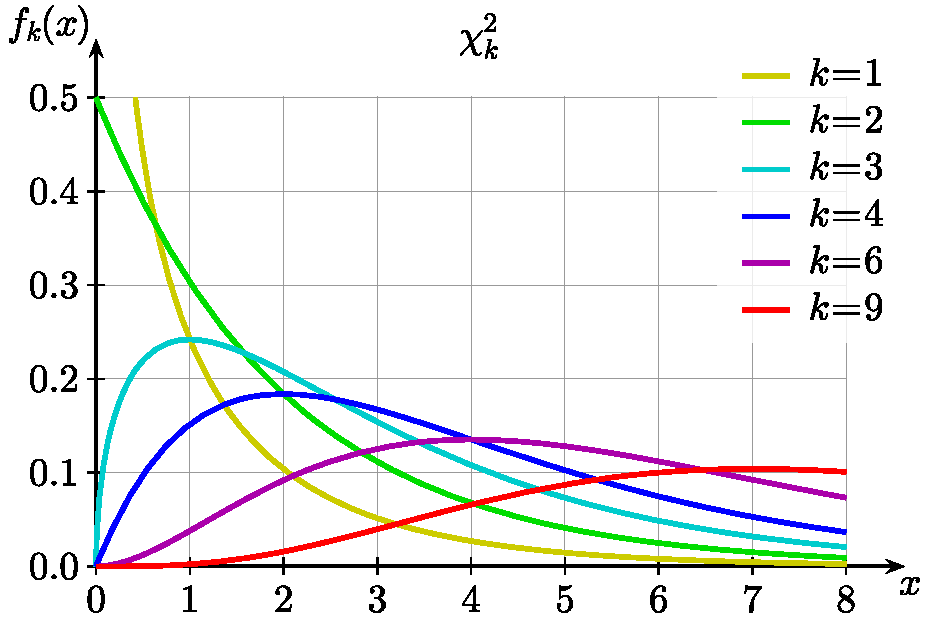
\includegraphics[width=0.7\textwidth]{../Diagrams/Chi-square.pdf}
  \caption{\ref{source:chi-squared} Illustration of how the \(\chi_{(\nu)}^2\) distribution looks with increasing degree of freedom \(\nu\).}
  \label{fig:chi-square}
\end{figure}
\begin{stbox}{General Information}
  \begin{itemize}
    \item Properties of chi-squared distributions.
    \begin{itemize}
      \item \(\E(X)=\nu\) and \(\Var(X)=2\nu\).
      % , and the mode of \(X\) is \(\max\{k-2,0\}\).
      \item The \(\chi_{(\nu)}^2\) distribution tends to a normal distribution as \(\nu\to\infty\).
      \item Suppose \(Z_i\sim\Normal(0,1)\) are independent. Then, \(Z_1^2+\dots+Z_n^2\sim\chi^2_{(n)}\).
      \item If \(X\sim\chi_{(\nu)}^2\) and \(Y\sim\chi_{(\upsilon)}^2\), then \(X+Y\sim\chi_{(\nu+\upsilon)}^2\).
    \end{itemize}
  \end{itemize}
\end{stbox}
\section{A Goodness-of-Fit Test}
\begin{stbox}{General Information}
    \begin{enumerate}
      \item Let [\(X\) in context].
      \item \emph{Note.} Use a pen to draw any necessary tables.

      \begin{tabular}{|ll|}
        \hline
        Test & \(H_0\colon\text{[\(X\) follows the distribution in context]}\)\\
        against &\(H_1\colon\text{[\(X\) does not follows the distribution in context]}\)\\
        \multicolumn{2}{|l|}{at the \(100\alpha\%\) significance level.}\\
        \hline
      \end{tabular}
      \item ~
      \begin{table}[H]
        \centering
        \begin{tabular}{|Sc|Sc|Sc|Sc|Sc|}
          \hline
          \(x\) & \(\leq x_1<\) & \(\leq x_2<\) & \(\cdots\) & \(\leq x_n<\)\\
          \hline
          \(f_i\) & \(f_1\) & \(f_2\) & \(\cdots\) & \(f_n\)\\
          \hline
          \(e_i\) & \(e_1\) & \(e_2\) & \(\cdots\) & \(e_n\)\\
          \hline
          \(\dfrac{(f_i-e_i)^2}{e_i}\) & \(\dfrac{(f_1-e_1)^2}{e_1}\) & \(\dfrac{(f_2-e_2)^2}{e_2}\) & \(\cdots\) & \(\dfrac{(f_n-e_n)^2}{e_n}\)\\
          \hline
        \end{tabular}
        \caption{Observed and expected frequencies for a goodness-of-fit test}
        \label{table:goodness-of-fit-test}
      \end{table}
      \item Check whether \(e_i\geq 5\) for each of the \(n\) classes. If it isn't, we need to combine \emph{just enough} adjacent classes, till they do. Working-wise, use some underbraces/overbraces to indicate the combined values. 
      \item Under \(H_0\), the test statistic is
      \[\chi^2=\sum{\frac{(F_i-E_i)^2}{E_i}}\sim\chi_{(\nu)}^2.\]
      Here, \(n\coloneq\#\text{classes}\) and \(\nu=(\#\text{classes}-\#\text{estimated parameters})-1\).
      \item Continue as per usual, calculating the critical region \(\chi_{(\nu)}^2>\chi^2_{(\nu,1-\alpha)}\) or the \(p\)-value.
    \end{enumerate}
\end{stbox}
\begin{GCSkills}{}
  \begin{itemize}
    \item To find the value of \(\chi^2_{(\nu,1-\alpha)}\), which satisfies \(\Prob\left(X>\chi^2_{(\nu,1-\alpha)}\right)=\alpha\), we use the table in the \href{https://www.seab.gov.sg/docs/default-source/national-examinations/syllabus/alevel/2022syllabus/List_MF26_y22_sy.pdf}{MF26 formula sheet (Page 9)}. Unfortunately, there is no inverse \(\chi^2\) function available.
    \item For the \(p\)-value:
    \begin{center}
      \texttt{stat} \(\Longrightarrow\) \texttt{TESTS} \(\Longrightarrow\) \texttt{D:\(\chi^2\)GOF-Test\dots}
    \end{center}
  \end{itemize}
\end{GCSkills}
\begin{note}
  If \(X\) follows a \emph{discrete} uniform distribution, we must state it out in words. We cannot write \(X\sim\operatorname{U}(\mu,\sigma^2)\) as this would denote that \(X\) is a \emph{continuous} random variable. But if \(X\sim\Binom(n,p)\) (or \(X\sim\Poisson(\lambda)\), etc), then we can just denote it as such. 
\end{note}
\begin{example}{\(\#\text{estimated parameters}=0\)}{}
  Given \(X\sim\Normal(0,1)\) (note how the \emph{population parameters} that define the distribution are \emph{known}), the degree of freedom \(\nu=n-1\).
\end{example}
\begin{example}{\(\#\text{estimated parameters}=1\)}{}
  Consider when \(X\sim\Binom(m,p)\), such that the expected frequency for each of the \(n\) classes is at least 5, but we do not know the exact value of \(p\). So, we \emph{estimate} it according to the sample given. Then, the degree of freedom is \(\nu=n-1-1=n-2\).
\end{example}
\begin{example}{\(\#\text{estimated parameters}=2\)}{}
  Similarly, suppose \(X\sim\Normal(\mu,\sigma^2)\), such that the expected frequency of each of the \(n\) classes is at least 5, and the true values of \(\mu\) and \(\sigma^2\) are unknown. In this case, the degree of freedom \(\nu=n-2-1=n-3\). 
\end{example}
\begin{note}
  Consider when we are testing 
\begin{center}
    \begin{tabular}{|ll|}
      \hline
      Test & \(H_0\colon X\sim\Normal(\mu,\sigma^2)\)\\
      against &\(H_1\colon X\not\sim\Normal(\mu,\sigma^2)\)\\
      \multicolumn{2}{|l|}{at the \(100\alpha\%\) significance level.}\\
      \hline
    \end{tabular} 
\end{center}
So, we want to fill up the values of \(e_i\) below.
\begin{table}[H]
  \centering
  \begin{tabular}{|Sc|Sc|Sc|Sc|Sc|}
    \hline
    \(x\) & \(a_1\leq x< a_2\) & \(a_2\leq x< a_3\) & \(\cdots\) & \(a_n\leq x\leq a_{n+1}\)\\
    \hline
    \(f_i\) & \(f_1\) & \(f_2\) & \(\cdots\) & \(f_n\)\\
    \hline
    \(e_i\) & \cellcolor{yellow} \(e_1\) & \(e_2\) & \(\cdots\) & \cellcolor{yellow} \(e_n\)\\
    \hline
  \end{tabular}
  \caption{Observed and expected frequencies when testing goodness-of-fit with a normal distribution.}
  \label{table:gof-normal} 
\end{table}
Let the sample size \(\sum f_i\) be \(m\). Then, we should calculate \(e_1=m\Prob(\highlight[green!50]{-\infty}<X< a_2)\) and \(e_n=m\Prob(a_n\leq X\leq \highlight[green!50]{\infty})\), instead of \(e_1=m\Prob(\highlight[red!30]{a_1}\leq X< a_2)\) or \(e_n=m\Prob(a_n\leq X\leq \highlight[red!30]{a_{n+1}})\). Similarly, for goodness-of-fit tests with Poisson and Geometric distributions, we must also be careful in ensuring that we account for \emph{all} possible values which \(X\) can take on, in calculating \(e_i\).
\end{note}
\begin{note}
  Suppose we are given a question of the following form.

  \vspace{-0.5\baselineskip}\rule{20cm-137.0549pt}{0.05mm}

  Some context\dots 
  \begin{table}[H]
    \centering
    \begin{tabular}{|Sc|Sc|Sc|Sc|Sc|}
      \hline
      \(x_i\) & \(x_1\) & \(x_2\) & \(\cdots\) & \(x_n\)\\
      \hline
      \(f_i\) & \(f_1\) & \(f_2\) & \(\cdots\) & \(f_n\)\\
      \hline
    \end{tabular}
    \caption{Some data.}
    \label{table:some-chi-data}
  \end{table}
  \begin{enumerate}[label=(\roman*)]
    \item Show, at the \(100\alpha\)\% significance level, that the data does not support the hypothesis of \(X\sim\operatorname{Geo}(p)\) with \(p=0.5\).
    \item State how the test in (i) would have to be amended to test the hypothesis of a geometric distribution for an \emph{unspecified value of \(p\)}.
  \end{enumerate}

  \rule{20cm-137.0549pt}{0.05mm}
  Then, for (ii), two main changes have to be made:
  \begin{enumerate}
    \item Estimate the value of \(p\) by computing the sample mean \(\widebar{x}\) and letting \(p=1/\widebar{x}\).
    \item Adjust the degree of freedom from 4 to \(4-1=3\), as there is one more restriction, that the mean must agree.
  \end{enumerate}
  (The phrasing is similar for gof tests for other distributions; simply use the appropriate estimators for the unknown population parameters.)
\end{note}
\begin{note}
  The \(\chi^2\) goodness-of-fit test showed that there is strong evidence for \(X\sim\Poisson(\lambda)\). Suggest a possible reason.

  % \rule{20cm-137.0549pt-25pt}{0.05mm}
  % \vspace{0.5\baselineskip}
  \[s^2=\rule{0.5cm}{0.05mm} \qquad \widebar{x}=\rule{0.5cm}{0.05mm}\]
  Since \(\widebar{x}\approx s^2\), the population mean and population variance of the [\(X\) in context] may be approximately equal. This made the data a good fit to the Poisson distribution.
\end{note}
\begin{note}
  Explain why a test based on a normal distribution might still be valid, despite the \(\chi^2\) test-of-independence implying that \(X\not\sim\Normal(\mu,\sigma^2)\).
  \begin{enumerate}
    \item The sample size of \rule{0.5cm}{0.01mm} is small. Hence, the result of the test may not accurately represent the population.
    \item{} [\(X\) in context] might still be normally distributed, but with \(\E(X)\neq\mu\) and/or \(\Var(X)\neq\sigma^2\).
  \end{enumerate} 
\end{note}
\section{Tests of Independence}
\begin{stbox}{General Information}
  \begin{enumerate}
    \item Let [\(X\) in context].
    \item 
    \begin{tabular}{|ll|}
      \hline
      Test & \(H_0\colon\text{[\(X\) in context] is independent of [\(Y\) in context]}\)\\
      against &\(H_1\colon\text{[\(X\) in context] is dependent on [\(Y\) in context]}\)\\
      \multicolumn{2}{|l|}{at the \(100\alpha\%\) significance level.}\\
      \hline
    \end{tabular}
    \item \emph{Note}. Unless the question asks for it, we do not need to write \(\left[ \frac{(f_i-e_i)^2}{e_i} \right]\) or its corresponding values, in the following table.
    \begin{table}[H]
      \hypertarget{table:tests-of-indepedence}{}
      \centering
      \begin{tabular}{ScSc|Sc|Sc|Sc|Sc|Sc}
        \cline{1-6}
        % &&\multicolumn{4}{Sc|}{\(X\)}&\\
        % \cline{3-7}
        % && \(x_1\) & \(x_2\) & \(\cdots\) & \(x_n\) & \multicolumn{1}{Sc|}{Total}\\
        \multicolumn{2}{|Sc|}{\multirow{2}{*}{\(f_i\) \((e_i)\) \(\left[ \frac{(f_i-e_i)^2}{e_i} \right]\)}} &\multicolumn{4}{Sc|}{\(X\)}&\\
        \cline{3-7}
        \multicolumn{2}{|Sc|}{}& \(x_1\) & \(x_2\) & \(\cdots\) & \(x_n\) & \multicolumn{1}{Sc|}{Total}\\
        \hline
        \multicolumn{1}{|Sc|}{\multirow{4}{*}{\(Y\)}}&\(y_1\)&&&&&\multicolumn{1}{Sc|}{\(t_{r_1}\)}\\ 
        \cline{2-7}
        \multicolumn{1}{|Sc|}{}&\(y_2\)&&&&&\multicolumn{1}{Sc|}{\(t_{r_2}\)}\\ 
        \cline{2-7}
        \multicolumn{1}{|Sc|}{}&\(\vdots\)&&&&&\multicolumn{1}{Sc|}{\vdots}\\
        \cline{2-7}
        \multicolumn{1}{|Sc|}{}&\(y_m\)&&&&&\multicolumn{1}{Sc|}{\(t_{r_m}\)}\\  
        \hline
        \multicolumn{1}{Sc|}{}& Total & \(t_{c_1}\) & \(t_{c_2}\) & \(\cdots\) & \(t_{c_n}\) & \multicolumn{1}{Sc|}{\(S=\sum{t_{r_i}}+\sum{t_{c_i}}\)}\\ 
        \cline{2-7}
      \end{tabular}
      \caption{\emph{Expected} frequencies for a test of independence.}
      \label{table:tests-of-indepedence}
    \end{table}
    % \Bigg(The expected frequencies are given by \(e_{ij}=\dfrac{\text{row total}\cdot\text{column total}}{\text{total number of observations}}=\dfrac{t_{r_i}t_{c_j}}{S}\).\Bigg)
    \vspace{-1em}
    \begin{minipage}{0.825\textwidth}
      \begin{remark}
        \hypertarget{test-of-independence-expected-frequencies}{}
        The expected frequencies are given by \(e_{ij}=\dfrac{\text{row total}\cdot\text{column total}}{\text{total number of observations}}=\dfrac{t_{r_i}t_{c_j}}{S}\).
      \end{remark}
    \end{minipage}
    \item Check whether \(e_i\geq 5\) for each of the \(mn\) cells. If it isn't, we need to combine \emph{just enough} adjacent classes, till they do. Working-wise, use some underbraces/overbraces/side braces to indicate the combined values. 
    \item Under \(H_0\), the test statistic is
    \[\chi^2=\sum{\frac{(F_i-E_i)^2}{E_i}}\sim\chi_{(\nu)}^2.\]
    Here, \(n\coloneq\#\text{cols}\) and \(\nu=(\#\text{rows}-1)(\#\text{cols}-1)\).
    \item Continue as per usual, calculating the critical region \(\chi_{(\nu)}^2>\chi^2_{(\nu,1-\alpha)}\) or the \(p\)-value.
  \end{enumerate}
\end{stbox}
\begin{GCSkills}{}
  Key in the matrix of observed frequencies: 
  \begin{center}
    \texttt{2nd} \(\Longrightarrow\) \(\texttt{x}^{-1}\) \(\Longrightarrow\) \texttt{EDIT} \(\Longrightarrow\) \texttt{[A]}.
  \end{center}
  Then, conduct the test for independence:
  \begin{center}
    \texttt{stat} \(\Longrightarrow\) \texttt{TESTS} \(\Longrightarrow\) \texttt{C:\(\chi^2\)-Test\dots}
  \end{center}
\end{GCSkills}
\begin{note}
  If it's unclear as to what is to be stated as independent/dependent in the hypotheses, consider the expected values and how they relate to the context.  
\end{note}
\begin{example}{}{}
  \label{eg:infering-independence-relation}
  Consider the following context:
  \begin{table}[H]
    \centering
    \begin{tabular}{ScSc}
      \toprule
      Statement & \textcolor{green!70!black}{Independent}/\textcolor{red}{Dependent}?\\
      \midrule
      There is consistency in the marking of the two T.A.s. & ?\\
      There is no consistency in the marking of the two T.A.s. & ?\\
      \bottomrule  
    \end{tabular}
    \caption{Two statements on the relationship between the marks awarded and the T.A. marking.}
    % , which can be confusing to interpret
    \label{table:NOT-FILLED-infering-independence-relation-hypotheses}
  \end{table}
  Then, under \(H_0\) --- the independence claim --- the expected frequencies are as stated below.
  \begin{table}[H]
    \centering
    \begin{tabular}{ScScScScSc}
      \toprule  
      \multicolumn{2}{Sc}{\multirow{2}{*}{\(e_{ij}\)}} & \multicolumn{3}{Sc}{Grade}\\
      && \(A\) & \(B\) & \(C\)\\
      \midrule
      \multirow{2}{*}{\rotatebox[origin=c]{90}{T.A.}} & \(X\) & \(a\) & \(b\) & \(c\)\\
      & \(Y\) & \(a\) & \(b\) & \(c\)\\
      \bottomrule
    \end{tabular}
    \caption{Expected frequencies.}
    \label{table:infering-independence-relation-data}
  \end{table}
  Since \(e_{1j}=e_{2j}\) for all \(1\leq j\leq 3\), we infer the following.
  \begin{table}[H]
    \centering
    \begin{tabular}{ScSc}
      \toprule
      Statement & \textcolor{green!70!black}{Independent}/\textcolor{red}{Dependent}?\\
      \midrule
      There is consistency in the marking of the two T.A.s. & \textcolor{green!70!black}{Independent}\\
      There is no consistency in the marking of the two T.A.s. & \textcolor{red}{Dependent}\\
      \bottomrule  
    \end{tabular}
    \caption{Which statement corresponds to independence and which coresponds to dependence.}
    \label{table:FILLED-infering-independence-relation-hypotheses}
  \end{table}
\end{example}
\begin{note}
  If the question says to ``use an approximate \(\chi^2\)-statistic\dots'', then we must use the critical region method. It is incorrect to use the \(p\)-value.
\end{note}
\begin{note}
  Consider when we are asked to state which cells correspond to the highest contributions to the test statistic, and relate that back to the context of the question. Then:
  \begin{enumerate}
    \item State the cells in the form (\rule{0.5cm}{0.05mm},\ \rule{0.5cm}{0.05mm}). E.g. (High, Good) and (Low, Good).
    \item In table \ref{table:tests-of-indepedence}, add an asterisk to each of these cells. E.g. 
    \begin{tabular}{|Sc|}
      \hline
      1 \((5)\) \([10.1]^{*}\)\\
      \hline
    \end{tabular}\ .
    \item Use words that imply correlation and \emph{not} causation. E.g. directly associated, correlates with, etc.
  \end{enumerate}
\end{note}
\begin{note}
  On a similar note, if the question asks ``Can it can be concluded that\dots'', but is unclear about whether it's implying correlation or causation, it may be safer to explain both ways. i.e. what correlation is there and why is there no causation. 
\end{note}
\begin{note}
  Explain why we cannot conclude any casual relationships from a test of independence.
  \begin{center}
    \parbox{0.9\textwidth}{
      No, the above test does not reflect the actual casual relationship between the two factors, if it exists. Rather, it merely suggests that they are not independent.
    }
  \end{center}
\end{note}
\begin{note}
  Explain why we cannot apply a \(\chi^2\)-test for independence using the data given.
  \begin{center}
    \parbox{0.9\textwidth}{
      The expeceted frequency for (\rule{0.5cm}{0.05mm},\ \rule{0.5cm}{0.05mm}) is \(\rule{0.5cm}{0.05mm}<5\). If we combine the columns, the degree of freedom \(\nu=1\cdot 0=0\). If we combine the rows, \(\nu=0\cdot 1=0\). Thus, we cannot apply a \(\chi^2\)-test for independence. 
    }
  \end{center}
\end{note}
\begin{note}
  Don't be intimidated when a question gives unknown \(f_i\)'s for multiple cells. By using the \hyperlink{test-of-independence-expected-frequencies}{formula} for \(e_i\), we should be able to rewrite them in terms of one unknown --- the observed frequency for one cell. Additional information should be provided, if this is not possible.
\end{note}
\chapter{Correlation and Linear Regression}
\section{Scatter Diagrams}
\begin{note}
  Guidelines for drawing a scatter diagram
  \begin{itemize}
    \item The relative position of each point on the scatter diagram should be clearly shown.
    \item The range of values for the set of data should be clearly shown by marking out the extreme \(x\) and \(y\) values on the corresponding axis.
    \item The axes should be labeled clearly with the variables.
  \end{itemize}
  \begin{figure}[H]
    \centering
    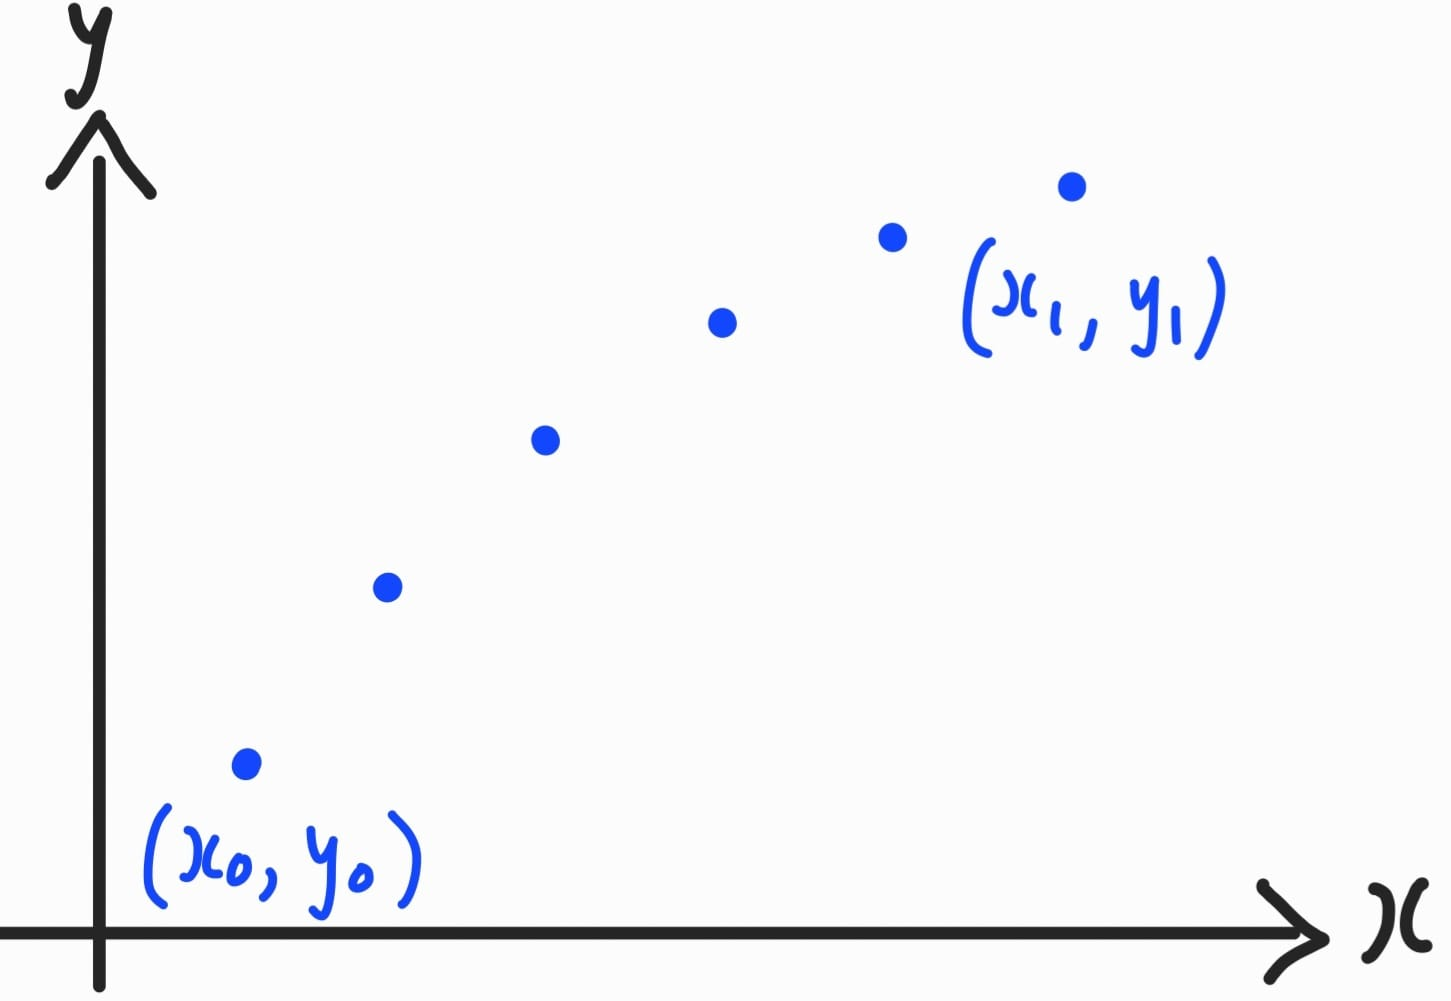
\includegraphics[width=0.4\textwidth]{../images/scatter-plot-example.jpg}
    \caption{\ref{Me} An illustration of a scatter plot.}
    \label{fig:example-scatter-plot-how-to-draw}
  \end{figure}
  \emph{Note.} We do not need to start from the origin.
\end{note}
\begin{GCSkills}{}
  To show a scatter plot on the G.C.:
  \begin{center}
    \texttt{2nd} \(\Longrightarrow\) \texttt{y=} \(\Longrightarrow\)  \texttt{1:Plot1\dots on} \(\Longrightarrow\) \texttt{enter} \(\Longrightarrow\)  \texttt{on}.
  \end{center} 
  \emph{Note.} When we no longer need a scatter plot, turn the scatter plot(s) \emph{off} in the G.C., lest it erroneously interferes with other functionalities of the G.C.
\end{GCSkills}
\begin{example}{}{}
  % N2008/II/8(iii)
  One of the values of \(t\) appears to be incorrect. Indicate the corresponding point on your diagram by labelling it \(P\) and explain why the scatter diagram for the remaining points may be consistent with a model of the form \(y=a+bf(x)\). 
  \begin{center}
    \parbox{0.9\textwidth}{
      With \(P\) removed, the remaning points seem to lie, on a curve that [e.g. increases at a decreasing rate], suggesting consistency with the model \(y=a+bf(x)\).
    }
  \end{center}
\end{example}
\section{Product Moment Correlation Coefficient \(r\)}
\begin{definition}{}{}
  The Product Moment Correlation Coefficient is a measure of the linear correlation between two variables. It is defined by
    \[r\coloneq\frac{\sum{(x-\widebar{x})(y-\widebar{y})}}{\sqrt{\sum{(x-\widebar{x})^2}\sum{(y-\widebar{y})^2}}}=\frac{\sum{xy}-\dfrac{\sum{x}\sum{y}}{n}}{\sqrt{\left[\sum{x^2}-\dfrac{\left(\sum{x}\right)^2}{n}\right]\left[\sum{y^2}-\dfrac{\left(\sum{y}\right)^2}{n}\right]}},\]
    and takes on a value from 0 to 1. See Figure \ref{fig:scatter-plot-r-value-examples} for some scatter plots of various \(r\) values.
    % \item When \(r=0\), there is no linear relationship. But, a nonlinear relationship may be present. Additionally, the regression lines are perpendicular.
    % \item The closer the value of \(r\) is to 1 (or \(-1\)), the stronger the positive (or negative) linear correlation. Furthermore, the regression lines coincide when \(\lvert r \rvert=1\).
\end{definition}
\begin{figure}[htbp]
  \centering
  \begin{subfigure}[c]{0.4\textwidth}
    \centering
    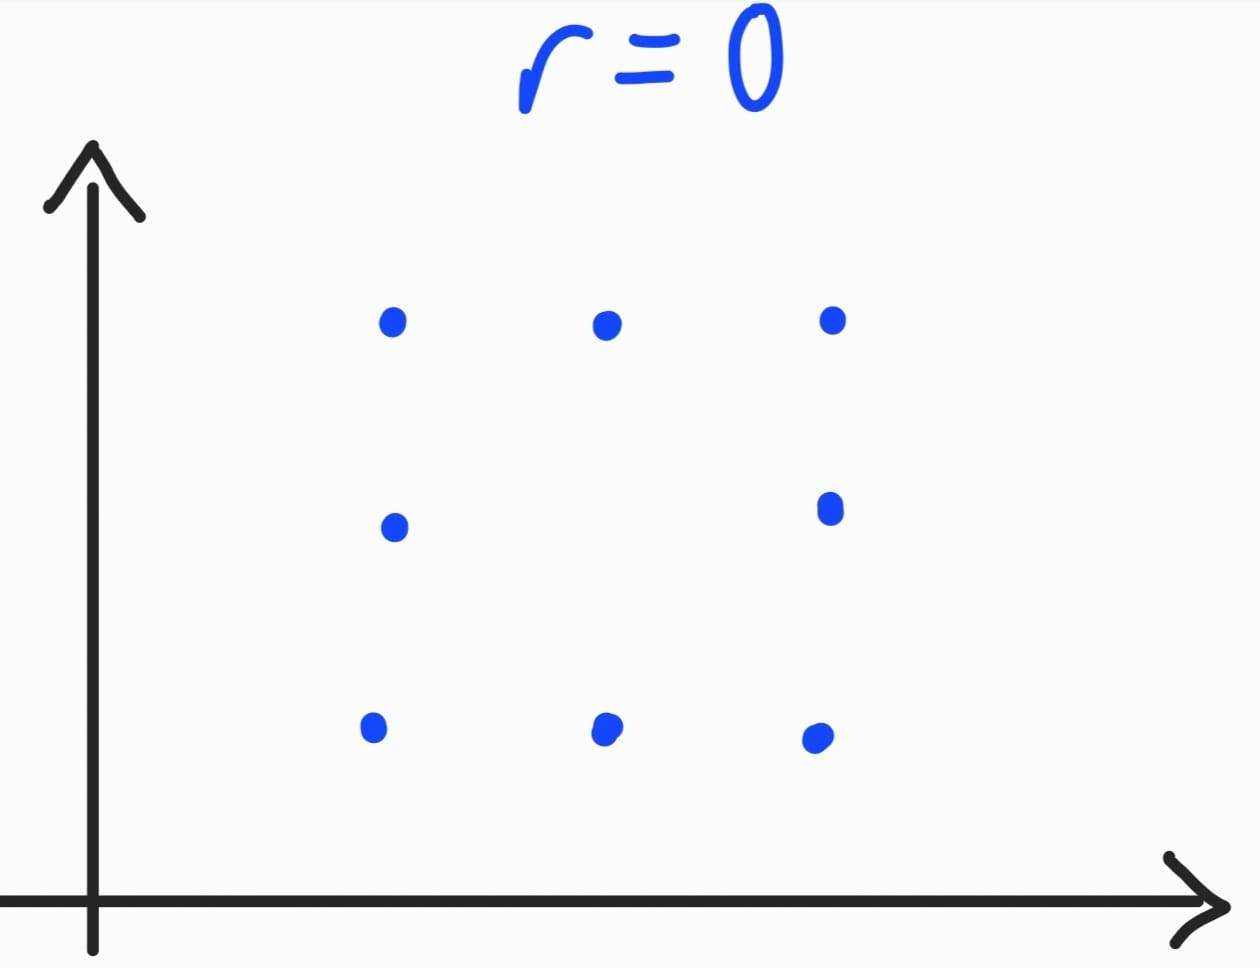
\includegraphics[width=\textwidth]{../images/product-moment-correlation-coefficient/r-is-0.jpg}
    \caption{No \emph{linear} relationship.}
  \end{subfigure}

  \begin{subfigure}[c]{0.4\textwidth}
      \centering
      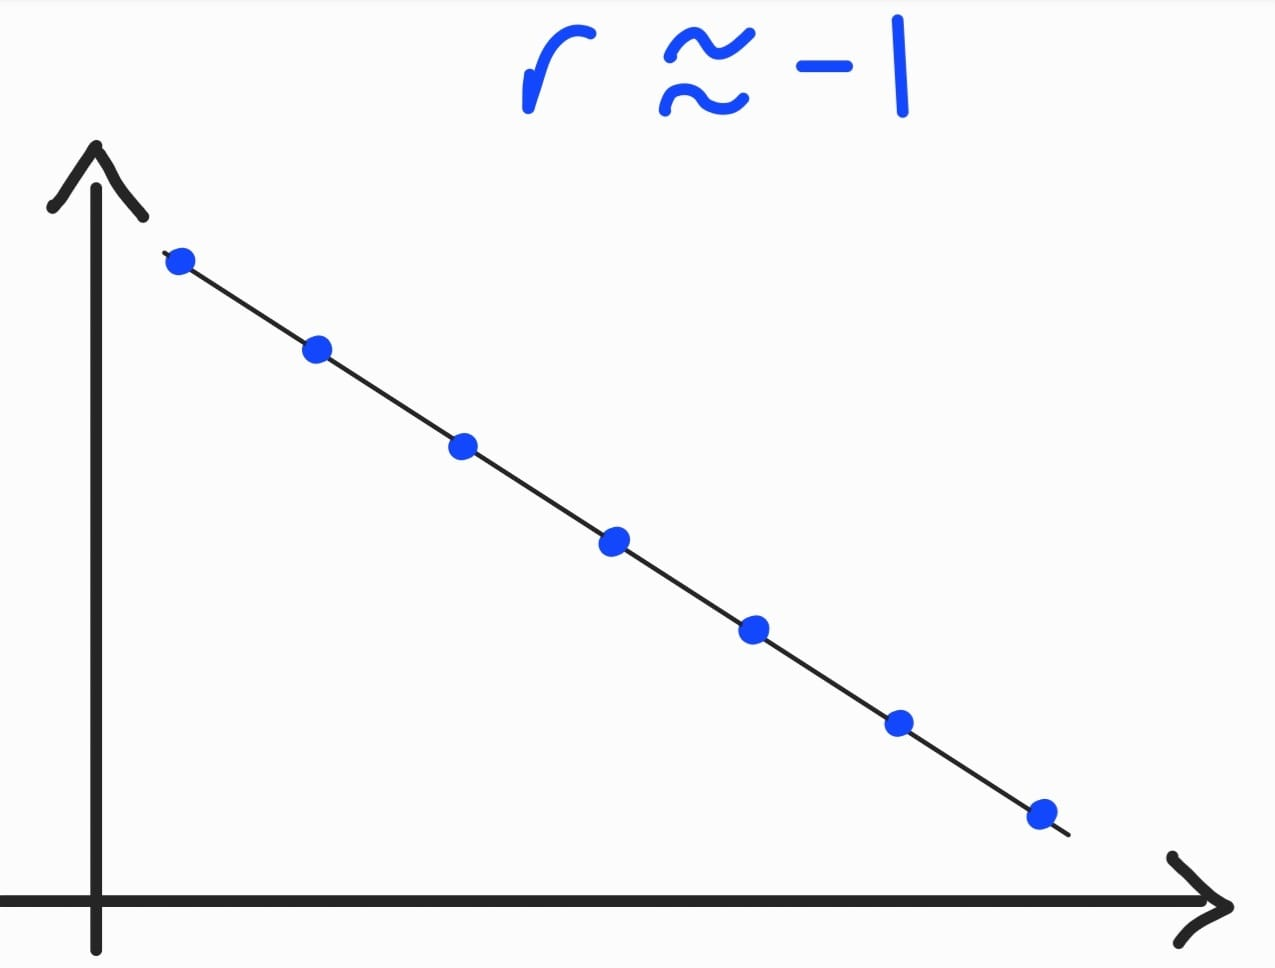
\includegraphics[width=\textwidth]{../images/product-moment-correlation-coefficient/r-is--neg-1.jpg}
      \caption{Strong negative linear relationship.}
  \end{subfigure}\hspace{0.06666666666667\textwidth}
  \begin{subfigure}[c]{0.4\textwidth}
      \centering
      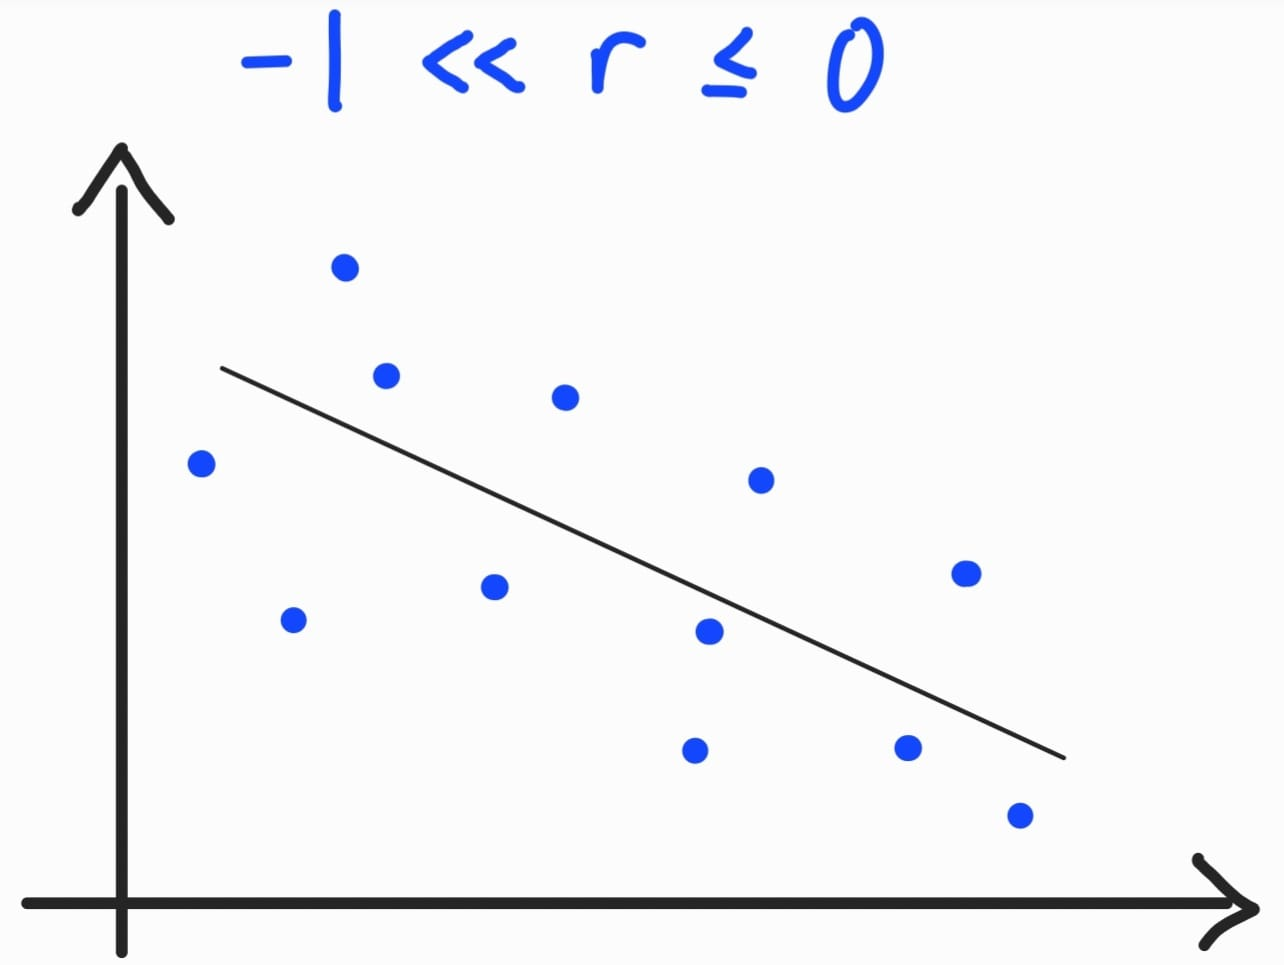
\includegraphics[width=\textwidth]{../images/product-moment-correlation-coefficient/small-negative-r.jpg}
      \caption{Weak negative linear relationship.}
  \end{subfigure}

  \begin{subfigure}[c]{0.4\textwidth}
      \centering
      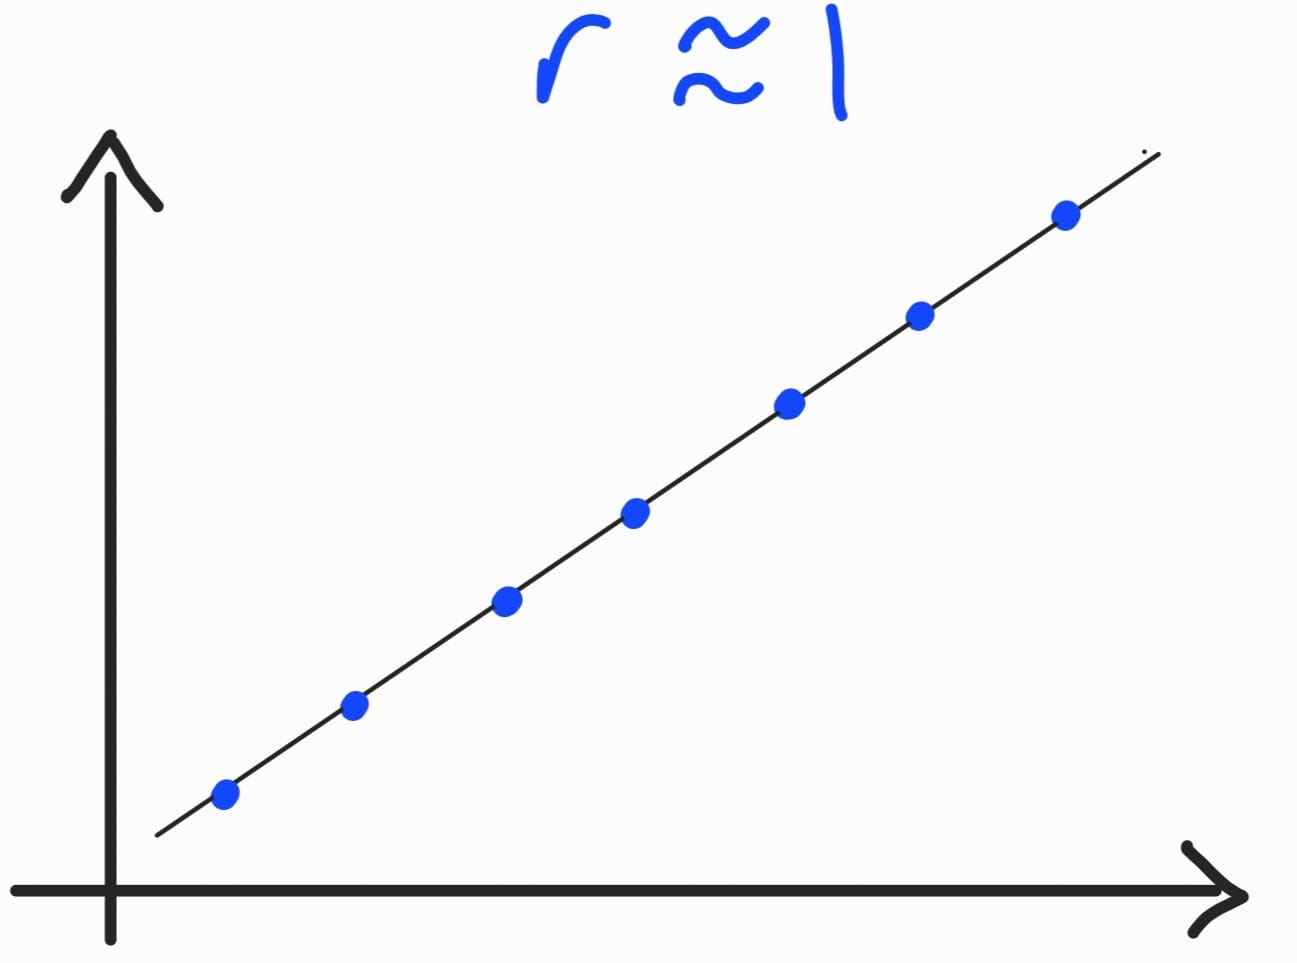
\includegraphics[width=\textwidth]{../images/product-moment-correlation-coefficient/r-is-1.jpg}
      \caption{Strong positive linear relationship.}
  \end{subfigure}\hspace{0.06666666666667\textwidth}
  \begin{subfigure}[c]{0.4\textwidth}
      \centering
      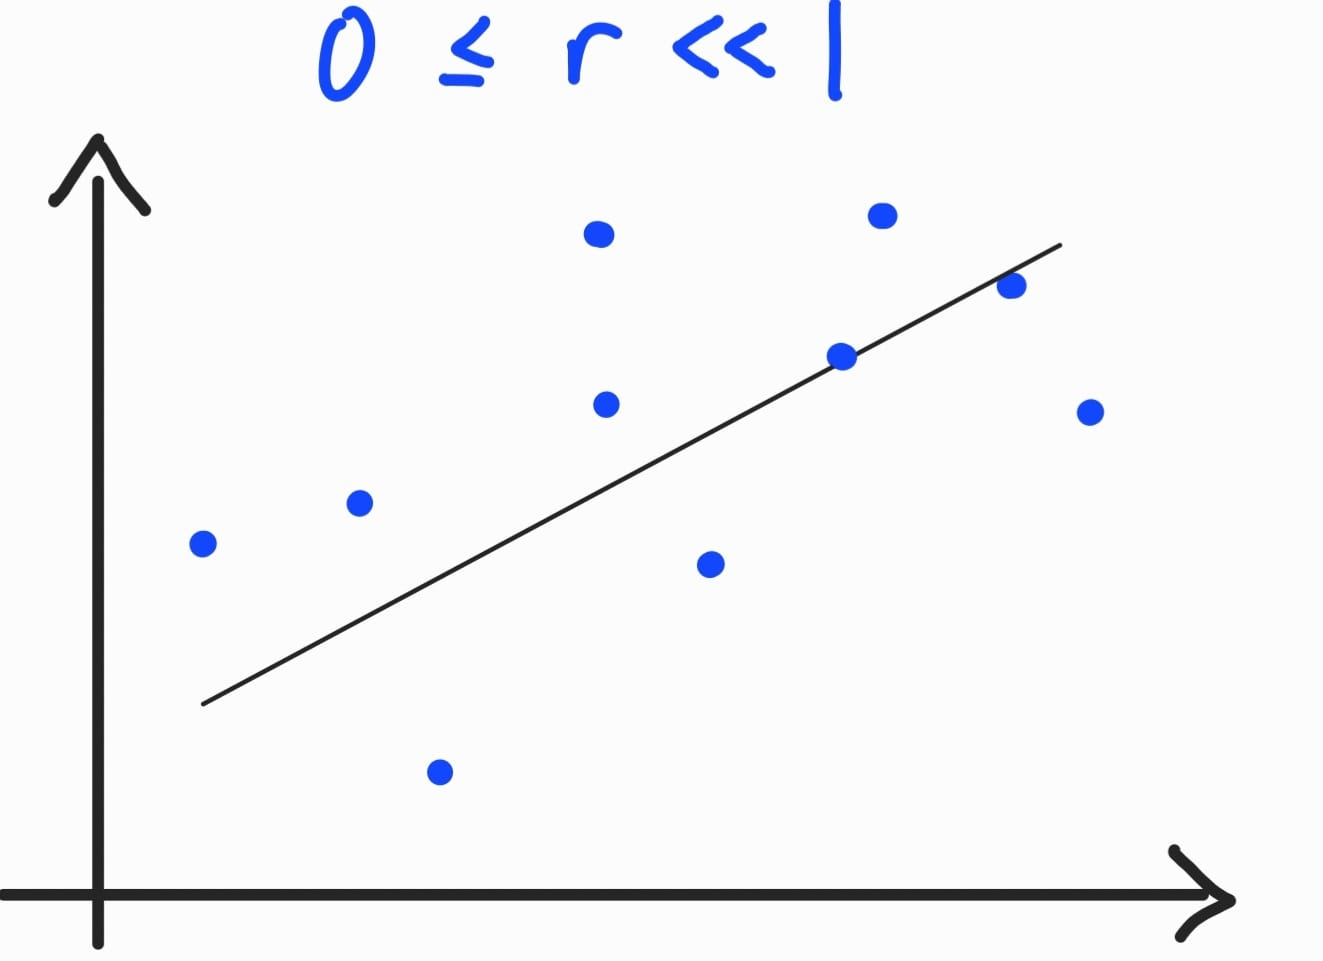
\includegraphics[width=\textwidth]{../images/product-moment-correlation-coefficient/small-positive-r.jpg}
      \caption{Weak positive linear relationship.}
  \end{subfigure}

  \begin{subfigure}[c]{0.4\textwidth}
    \centering
    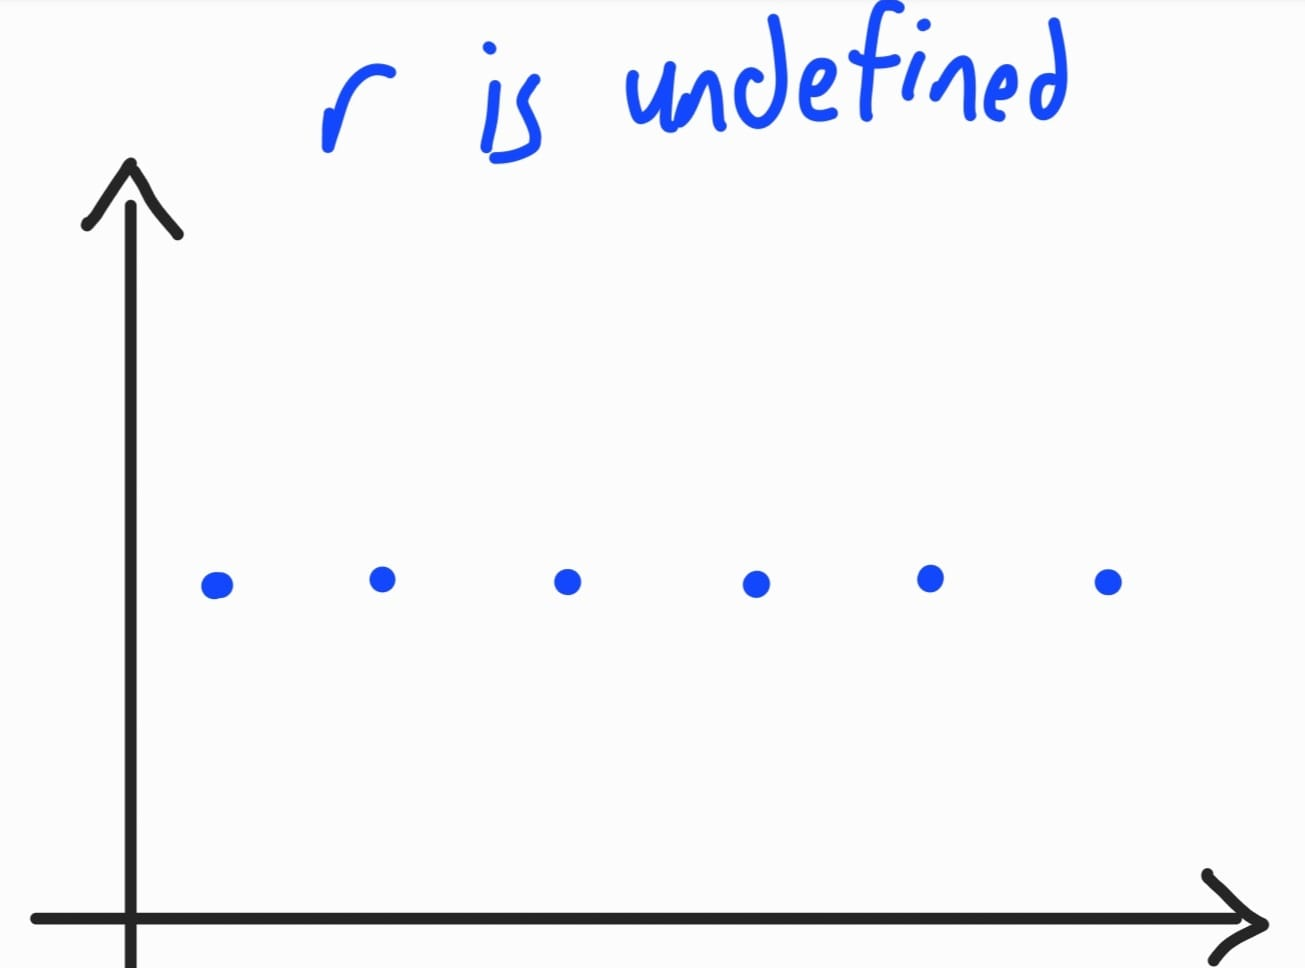
\includegraphics[width=\textwidth]{../images/product-moment-correlation-coefficient/r-is-undefined-horizontal-points.jpg}
    \caption{\(\sum{(y-\widebar{y})^2}=0\).}
  \end{subfigure}\hspace{0.06666666666667\textwidth}
  \begin{subfigure}[c]{0.4\textwidth}
    \centering
    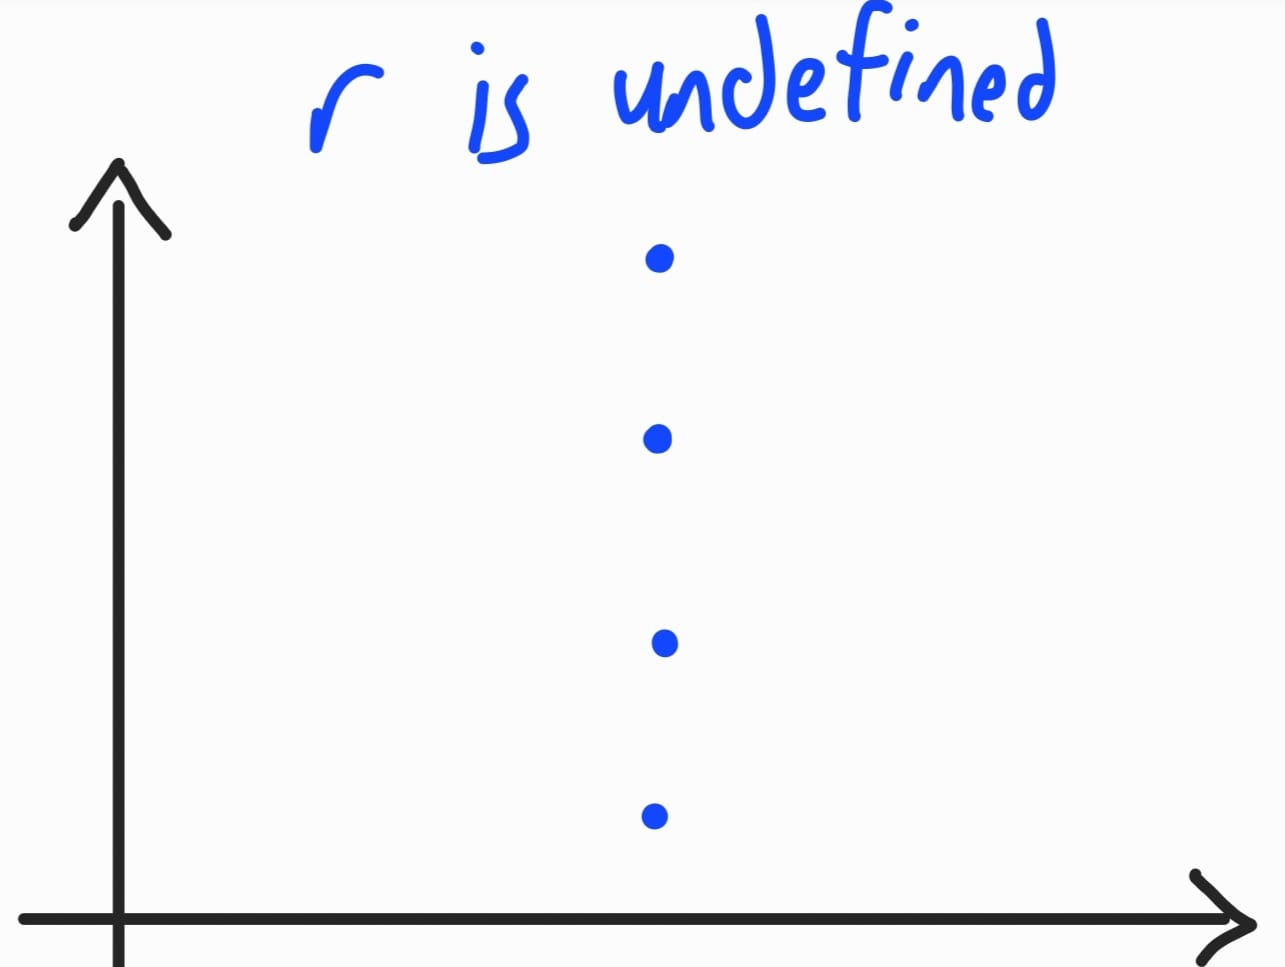
\includegraphics[width=\textwidth]{../images/product-moment-correlation-coefficient/r-is-undefined-vertical-points.jpg}
    \caption{\(\sum{(x-\widebar{x})^2}=0\).}
  \end{subfigure}
  \caption{\ref{Me} Example scatter plots with different values of \(r\).}
  \label{fig:scatter-plot-r-value-examples}
  \begin{flushleft}
    \emph{Note.} Even though there is no \emph{linear} relationship when \(r=0\), there might be a \emph{nonlinear} relationship present. 
  \end{flushleft}
\end{figure}
\begin{note}
  Explain whether your estimate using the regression line of \(y\) on \(x\) is reliable.
  \begin{center}
    \parbox{0.9\textwidth}{
      Since the \(\lvert r \rvert\) value of \rule{0.5cm}{0.01mm} is close to 1, \emph{and} \(x=\rule{0.5cm}{0.01mm}\) is within the data range of \(\rule{0.5cm}{0.01mm}\leq x\leq \rule{0.5cm}{0.01mm}\), the estimate is reliable.
    }
  \end{center}
\end{note}
\begin{note}
  Explain why the estimate using the regression line \(y\) on \(x\) is not reliable.
  \begin{center}
    \parbox{0.9\textwidth}{
      Since \(x=\rule{0.5cm}{0.01mm}\) falls outside of the range of data \(\rule{0.5cm}{0.01mm}\leq x\leq \rule{0.5cm}{0.01mm}\), we would be extrapolating the observed data points. This makes the estimate of the value of \(y\) at \(x=\rule{0.5cm}{0.01mm}\) unreliable.
    }
  \end{center}
\end{note}
\begin{note}
  Explain which dataset would result in a larger absolute value of the product moment correlation coefficient.
  \begin{itemize}
    \item Set \(A\) will have a larger \(\lvert r \rvert\) value, because its data points lie relatively \emph{closer to a straight line} (with positive/negative gradient), suggesting a stronger linear correlation.
    \item Set \(B\)'s \(\lvert r \rvert\) value will be closer to zero, since its data points are \emph{more scattered}, suggesting a weaker linear correlation. 
  \end{itemize}
\end{note}
\section{Regression Lines}
\begin{stbox}{General Information}
  The regression line of \(y\) on \(x\) minimises the sum of squares deviation (error) in the \(y\)-direction --- we assume that \(x\) is the independent variable whose values are known exactly. It is given by
  \[y=\widebar{y}+b(x-\widebar{x}),\qquad\text{where}\qquad b\coloneq\frac{\sum{(x-\widebar{x})(y-\widebar{y})}}{\sum{(x-\widebar{x})^2}}=\frac{\sum{xy}-\dfrac{\sum{x}\sum{y}}{n}}{\sum{x^2}-\dfrac{\left(\sum{x}\right)^2}{n}}.\] 
\end{stbox}
\begin{GCSkills}{}
  To find the \(r\)-value, or the regression line of \(y\) on \(x\), for a given dataset:
  \begin{center}
    \texttt{stat} \(\Longrightarrow\) \texttt{CALC} \(\Longrightarrow\) \texttt{4:LinReg(ax+b)}\quad or\quad \texttt{8:LinReg(a+bx)}
  \end{center}
\end{GCSkills}
\begin{note}
  With the aid of diagrams, explain the difference between the least square regression lines of \(y\) on \(x\) and that of \(x\) on \(y\).
  
  \rule{20cm-137.0549pt}{0.05mm}

  \begin{minipage}{0.475\textwidth}
    \begin{figure}[H]
      \centering
      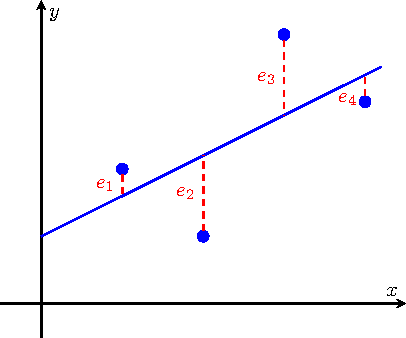
\includegraphics[width=\textwidth,page=1]{../Diagrams/least-square-regression-line/regression-line.pdf}
      \caption{\ref{Me} \ref{source:conics2} Regression line of \(y\) on \(x\).}
      \label{fig:y-on-x}
    \end{figure}
    The regression line of \(y\) on \(x\) assumes that the values of \(x\) are known exactly and to perfect accuracy. As such, it minimises the sum of squared \textcolor{red}{distances}, \(\sum{\textcolor{red}{e_i}^2}\) in the \(y\)-direction, as shown above.
  \end{minipage}\hfill
  \begin{minipage}{0.475\textwidth}
    \begin{figure}[H]
      \centering
      \includegraphics[width=\textwidth,page=2]{../Diagrams/least-square-regression-line/regression-line.pdf}
      \caption{\ref{Me} \ref{source:conics2} Regression line of \(x\) on \(y\).}
      \label{fig:x-on-y}
    \end{figure}
    The regression line of \(x\) on \(y\) assumes that the values of \(y\) are known exactly and to perfect accuracy. As such, it minimises the sum of squared \textcolor{red}{distances}, \(\sum{\textcolor{red}{e_i}^2}\) in the \(x\)-direction, as shown above.
  \end{minipage}
\end{note}
\begin{example}{}{}
  Show on the scatter diagram in part (d) the distances which are used in drawing the least squares regression line of \(y\) on \(x\). Explain why these distances are squared, and why this is referred to as the `method of least squares'.

  \rule{20cm-137.0549pt}{0.05mm}
  \begin{figure}[H]
      \centering
      \includegraphics[width=0.475\textwidth,page=3]{../Diagrams/least-square-regression-line/regression-line.pdf}
      \caption{\ref{Me} \ref{source:conics2} Regression line of \(y\) on \(x\).}
      \label{fig:least-squares}
  \end{figure}
  \begin{itemize}
    \item The \textcolor{red}{distances} are signed, i.e. can be positive or negative. 
    \item So, squaring the \textcolor{red}{distances} ensures the sum will not become zero (unless the plotted points are collinear) or negative.
    \item The least squares regression line is the line for which the sum of squared \textcolor{red}{distances} is minimised. Hence, this is referred to as the `method of least squares'
  \end{itemize} 
\end{example}
\begin{example}{}{}
  % N2003/II/11
  Suppose that we are given pairs of data for \(x\) and \(y\), as shown below:
  \begin{table}[H]
    \centering
    \begin{tabular}{ScScScScSc}
      \toprule
      \(x\) & \(x_1\) & \(x_2\) & \(\cdots\) & \(x_n\)\\
      \midrule
      \(y\) & \(y_1\) & \(y_2\) & \(\cdots\) & \(y_n\)\\
      \bottomrule
    \end{tabular}
    \caption{A dataset of \(n\) pairs of \(x\) and \(y\) values.}
  \end{table} 
  Let \(Y\) be the value obtained by substituting a sample value of \(x\) into the equation of the regression line of \(y\) on \(x\), given by \(Y=ax+b\). Consider any \(Y'=\alpha x+\beta\). What can you say about the value of \(\sum{(y-Y')^2}\)?

  \rule{\textwidth}{0.05mm}\vspace{0.5\baselineskip}
  Since \(\sum{(y-Y')^2}\) is minimised when \(Y'=ax+b\), we see that \(\sum{(y-Y')^2}\geq\sum{(y-Y)^2}\) for any \(Y'=\alpha x+\beta\).
\end{example}
\begin{note}
  The regression lines of \(y\) on \(x\) and \(x\) on \(y\) intersect at \((\widebar{x},\widebar{y})\).
\end{note}
\begin{note}
  To estimate the value of a variable \(y\), given a the value of another variable \(x\), we always use the regression line of the \hl[green!25]{\emph{dependent} variable} on the \hl[blue!15]{\emph{independent} variable}.
  \begin{table}[H]
    \centering
    \begin{tabular}{>{\columncolor{blue!15}}Sc>{\columncolor{green!25}}ScSc}
      \toprule
      Independent variable & Dependent variable & Regression line\\
      \midrule
      \(x\) & \(y\) & \(\highlight[green!25]{y}\) on \(\highlight[blue!15]{x}\)\\
      \(y\) & \(x\) & \(\highlight[green!25]{x}\) on \(\highlight[blue!15]{y}\)\\
      \bottomrule
    \end{tabular}
    \caption{Regression line to use for estimations.}
    \label{table:regression-line-indepedent-dependent-variable}
  \end{table}
\end{note}
\begin{note}
  Explain why a linear model would not be appropriate. Choose any relevant ones.
    \begin{itemize}
      \item The scatter diagram/data indicates that, as \(x\) increases, \(y\) [e.g. increases at a decreasing rate], which is \emph{not} a linear relationship.
      \item A linear model will increase \emph{indefinitely} with more [\(x\) in context]. This is contextually \emph{unrealistic}, as [reason in context]. 
      \item A linear model would imply that, in the long run, the [e.g. time taken] would be negative, which is impossible.
    \end{itemize}
\end{note}
\begin{note}
  By calculating the product moment correlation coefficients, explain whether model \(y=ax+b\) or model \(\mathbf{y}=\mathbf{a}\mathbf{x}+\mathbf{b}\) is more appropriate.
  \begin{center}
    \parbox{0.9\textwidth}{
      The \(\lvert r \rvert\) value for the model \(y=ax+b\) is higher at \rule{0.5cm}{0.01mm}, compared to \rule{0.5cm}{0.01mm} for the model \(\mathbf{y}=\mathbf{a}\mathbf{x}+\mathbf{b}\). Thus, there is a stronger (positive/negative) correlation between \(x\) and \(y\). As such, the model \(y=ax+b\) is more appropriate.
    }
  \end{center}
\end{note}
\begin{note}
  Let \(x\) be in unit\(_x\) and \(\mathbf{x}\) be in unit\(_{\mathbf{x}}\). Suppose that the \(c\text{ unit}_x=1\text{ unit}_\mathbf{x}\), where \(c\) is a constant. Then, if \(y=ax+b\), we have \(y=ac\mathbf{x}+b\).
\end{note}
\section{Other Notes}
\begin{note}
  Explain whether it is valid to conclude that a higher value of \(x\) will \emph{result in} a lower/higher value of \(y\).
  
  \begin{center}
    \parbox{0.9\textwidth}{
      No. While a higher value of \(x\) is \emph{correlated} with a higher value of \(y\), this does not imply any \emph{causal} relationship between \(x\) and \(y\).
    }
  \end{center}
  \emph{Note.} ``result in'' tends to refer to a \emph{causal} relationship.
\end{note}
\begin{example}{}{}
  Suggest an improvement to the data collection process so that the results could provide a fairer gauge of the expected outcome.
  \begin{center}
    \parbox{0.9\textwidth}{
      The randomly selected [members of population] might have been of different [category 1; e.g. gender] and [category 2; e.g. age]. To make the results fairer, the data could have been separated based on [category 1] and [category 2].
    }
  \end{center}
\end{example}
\chapter{Non-Parametric Tests}
\section{Sign Test}
\begin{stbox}{General Information}
  \begin{itemize}
    \item A \emph{sign test}.
    \begin{enumerate}
      \item Let \(m\) be the population median of \(D=\rule{1.5cm}{0.01mm}-\rule{1.5cm}{0.01mm}\).
      \item 
      \begin{tabular}{|ll|}
        \hline
        Test & \(H_0\colon m=m_0\)\\
        against &\(H_1\colon\) 
        \begin{enumerate*}[itemjoin={\quad}]
          \item \(m<m_0\),
          \item \(m\neq m_0\),\quad or
          \item \(m>m_0\),
        \end{enumerate*}\\
        \multicolumn{2}{|l|}{at the \(100\alpha\%\) significance level.}\\
        \hline
      \end{tabular}
      \item ~
      \begin{table}[H]
        \centering
        \begin{tabular}{|Sc|Sc|Sc|Sc|Sc|Sc|}
          \hline
          [label in context] & 1 & 2 & 3 & \(\cdots\) & \(N\)\\
          \hline 
          Sign & \(+\) & \(0\) & \(-\) & \(\cdots\) & \(+\)\\
          \hline
        \end{tabular}
        \caption{The signs of \(d_1,d_2,\dots,d_N\), for a sign test. Instead of \(1,2,\dots,N\) the labeling/column headers can differ in the given context. E.g. \(A,B,\dots,K\). Similarly, the signs here are mere examples; the \(i\)th sign cell should be filled with \(+\) (\(-\)) [0] if \(\operatorname{sgn}(d_i)=1\) (\(=-1\)) [\(=0\)].}
        \label{table:sign-test-working-table}
      \end{table}
      \item Let \(X_{+}\) be the number of \(`+'\). Under \(H_0\), \(X_{+}\sim\Binom(\hyperlink{non-parametric-tests-n-value}{n},1/2)\), \(x_{+}=\rule{0.5cm}{0.01mm}\). (Alternatively, \(X_{-}\) can also be used.)
      \item Since \(p\text{-value}=\rule{1cm}{0.01mm}<100\alpha\%\) (\(\geq 100\alpha\%\)), there is sufficient (insufficient) evidence, at the \(100\alpha\%\) significance level, to conclude that [\(H_1\) in context].
    \end{enumerate}
    \item \emph{Note.} The \(p\)-value for a sign test is given by
    \begin{table}[H]
      \centering
      \begin{tabular}{ScScScSc}
        \toprule
        \(H_1\) & \(m<m_0\) & \(m>m_0\) & \(m\neq m_0\)\\
        \midrule
        \(X_{+}\) & \(\Prob(X_{+}\leq x_{+})\) & \(\Prob(X_{+}\geq x_{+})\) & \(2\min\{\Prob(X_{+}\geq x_{+}),\Prob(X_{+}\leq x_{+})\}\)\\
        \midrule
        \(X_{-}\) & \(\Prob(X_{-}\geq x_{-})\) & \(\Prob(X_{-}\leq x_{-})\) & \(2\min\{\Prob(X_{-}\geq x_{-}),\Prob(X_{-}\leq x_{-})\}\)\\
        \bottomrule
      \end{tabular}
      \caption{The \(p\)-value for a sign test.}
      \label{table:sign-test-p-value}
    \end{table}
  \end{itemize}
\end{stbox}
\begin{note}
  Sign test. Suppose we have \(H_1\colon m\neq m_0\). To find the range of values of \(x_{+}\) that result in the rejection of \(H_0\), use GC to compute the following tables.
  \begin{table}[H]
    \centering
    \begin{tabular}{|Sc|Sc|}
      \hline
      \(x_{+}\) & \(\alpha/2-2\Prob(X_{+}\leq x_{+})\)\\
      \hline
      \(n-1\) & \(\rule{0.5cm}{0.01mm}>0\)\\
      \hline
      \(n\) & \(\rule{0.5cm}{0.01mm}>0\)\\
      \hline
      \(n+1\) & \(\rule{0.5cm}{0.01mm}<0\)\\
      \hline
    \end{tabular}\hspace{1cm}
    \begin{tabular}{|Sc|Sc|}
      \hline
      \(x_{+}\) & \(\alpha/2-2\Prob(X_{+}\geq x_{+})\)\\
      \hline
      \(N-1\) & \(\rule{0.5cm}{0.01mm}<0\)\\
      \hline
      \(N\) & \(\rule{0.5cm}{0.01mm}<0\)\\
      \hline
      \(N+1\) & \(\rule{0.5cm}{0.01mm}>0\)\\
      \hline
    \end{tabular} 
  \end{table}
  Then, we conclude that \(x_{+}\leq n\) or \(x_{+}\geq N\).
\end{note}
\section{Wilcoxon Matched-Pairs Signed Rank Test}
\begin{note}
  Assumptions needed for the Wilcoxon Matched-Pairs Signed Rank Test:
  \begin{enumerate}
    \item The data within each pair are dependent on each other, but pairs are independent of each other.
    \item The distribution of the differences is continuous and symmetrical.
  \end{enumerate}
\end{note}
\begin{stbox}{General Information}
  \begin{itemize}
    \item A Wilcoxon matched-pairs signed rank test. 
    \begin{enumerate}
      \item Let \(m\) be the population median of \(D=\rule{1.5cm}{0.01mm}-\rule{1.5cm}{0.01mm}\).
      \item 
      \begin{tabular}{|ll|}
        \hline
        Test & \(H_0\colon m=0\)\\
        against &\(H_1\colon\) 
        \begin{enumerate*}[itemjoin={\quad}]
          \item \(m<\highlight[yellow]{0}\),
          \item \(m\neq \highlight[yellow]{0}\),\quad or
          \item \(m>\highlight[yellow]{0}\),
        \end{enumerate*}\\
        \multicolumn{2}{|l|}{at the \(100\alpha\%\) significance level.}\\
        \hline
      \end{tabular}
      \item ~
      \begin{table}[H]
        \centering
        \begin{tabular}{|Sc|Sc|Sc|Sc|Sc|Sc|}
          \hline
          [label in context] & 1 & 2 & 3 & \(\cdots\) & \(N\)\\
          \hline 
          \(d\) & \(d_1\) & \(0\) & \(d_3\) & \(\cdots\) & \(d_N\)\\
          \hline
          Rank & \(1\) & \(0\) & \(5\) & \(\cdots\) & \(2\)\\
          \hline
        \end{tabular}
        \caption{The value of the differences \(d_1,d_2,\dots,d_N\), which are then ranked according to their absolute size \(\lvert d_i \rvert\). For our syllabus, each \(d_i\) is always distinct.
        % When the absolute difference is identical across two or more columns, \protect\hyperlink{tied-ranks-example}{take the average rank}.
        }
        \label{table:wilcoxon-working-table}
      \end{table}
    \end{enumerate}
    \begin{minipage}{0.6\textwidth}
      \begin{enumerate}
        \setcounter{enumi}{3}
        \item
        \begin{itemize}[label=\(\circ\)]
          \item \(t_{-}=\rule{0.5cm}{0.01mm}+\rule{0.5cm}{0.01mm}+\dots+\rule{0.5cm}{0.01mm}=\rule{0.5cm}{0.01mm}\)
          \item \(t_{+}=\rule{0.5cm}{0.01mm}+\rule{0.5cm}{0.01mm}+\dots+\rule{0.5cm}{0.01mm}=\rule{0.5cm}{0.01mm}\)
          \item The test statistic is \(T\coloneq\min\{T_{-},T_{+}\}=\rule{0.5cm}{0.01mm}\).
          \item Reject \(H_0\) if \(T=\rule{0.5cm}{0.01mm}\). (see table \ref{table:wilcoxon-critical-region})
        \end{itemize}
      \end{enumerate}
    \end{minipage}%
    \hspace{0.15cm}
    \begin{minipage}{0.3\textwidth}
      \begin{remark}
        \[\frac{\hyperlink{non-parametric-tests-n-value}{n}(\hyperlink{non-parametric-tests-n-value}{n}+1)}{2}=t_{-}+t_{+}.\]
      \end{remark}
      \vspace{0.7cm}
    \end{minipage}
    \begin{enumerate}
      \setcounter{enumi}{4}
      \item Since \(t=\rule{0.5cm}{0.01mm}\,\square\, \rule{0.5cm}{0.01mm}\), there is sufficient/insufficient evidence, at the \(100\alpha\%\) significance level, to conclude that [\(H_1\) in context].
    \end{enumerate}
    \item The test statistics \(T_{+}\) and \(T_{-}\) can also be used, depending on our preference.
      \item The critical regions for a Wilcoxon test, for each alternative hypothesis and test statistic \(T_{-}\) or \(T_{+}\). The value of \(c\) is obtained from MF26\(^{\hyperlink{non-parametric-tests-n-value}{*}}\). 
      
      \emph{Note.} the value of \(c\) may differ for a one-tail vs a two-tail test, so look at the table carefully, to obtain the correct value.
      \begin{table}[H]
        \centering
        \setlength{\tabcolsep}{12pt}
        \begin{tabular}{ScScScSc}
          \toprule
          \(H_1\) & \(m<0\) & \(m>0\) & \(m\neq 0\)\\
          \midrule
          \(T_{+}\) & \(T_{+}\leq c\) & \(T_{+}\geq \dfrac{n(n+1)}{2}-c\) & \(T_{+}\leq c\)\quad or\quad\(T_{+}\geq \dfrac{n(n+1)}{2}-c\)\\
          \midrule
          \(T_{-}\) & \(T_{-}\geq \dfrac{n(n+1)}{2}-c\) & \(T_{-}\leq c\) & \(T_{-}\leq c\)\quad or\quad\(T_{-}\geq \dfrac{n(n+1)}{2}-c\)\\
          \midrule
          \(T\) & \multicolumn{2}{Sc}{\(T\leq c^{\hyperlink{wilcoxson-T=min-note}{1}}\)} & \(T\leq c\)\quad or\quad\(T\geq \dfrac{n(n+1)}{2}-c\)\\
          \bottomrule
        \end{tabular}
        \caption{The critical regions for Wilcoxon tests.}
        \label{table:wilcoxon-critical-region}
      \end{table}
      \begin{footnotesize}
        {}\(^{\protect\hypertarget{wilcoxson-T=min-note}{1}}\)Assuming \(T_{-}\geq T_{+}\) for \(m<0\), and \(T_{+}\geq T_{-}\) for \(m>0\).
      \end{footnotesize}
      \setlength{\tabcolsep}{6pt}
      \item For large sample sizes \(n\geq 21\), we use the approximation 
      \[T\sim\Normal\left( \frac{n(n+1)}{4},\frac{n(n+1)(2n+1)}{24} \right)\]
      and conduct a one/two-tailed \(z\)-test.
  \end{itemize}
\end{stbox}
\begin{GCSkills}{}
  After calculating our list of differences \texttt{L\(_3\)}, we can calculate \(\texttt{L}_4=\lvert \texttt{L}_3 \rvert\) and use the G.C. to rank this list in ascending order:
  \begin{center}
    \texttt{stat} \(\Longrightarrow\) \texttt{2:SortA} \(\Longrightarrow\) \(\texttt{L}_4\).
  \end{center}
  This allows us to easily compute the ranks associated with each difference.
\end{GCSkills}
% \begin{note}
%   \hypertarget{tied-ranks-example}{}
%   Suppose wlog that \(0<\lvert d_1 \rvert<\lvert d_2 \rvert<\dots<\lvert d_p \rvert<\lvert d \rvert<\lvert d_{q+1} \rvert<d_{q+2}<\dots<d_n\) in the following table. Then, the rank assigned to the columns with identical absolute difference \(d\) is \(\highlight[black!15]{r\coloneq\frac{1}{q-p}\sum_{i=p+1}^{q}{i}}\):
%   % that \(\lvert d \rvert,\lvert d_1 \rvert,\lvert d_2 \rvert,\dots\) are unique and nonzero. Further assume that there is a one-to-one correspondence between \(\{r_1,r_2,\dots,r_p\}\cup\{r_{q+1},r_{q+2},\dots,r_n\}\) and \(\{1,2,\dots,s-1\}\cup\{s-p+q,s-p+q+1,\dots,n\}\). Then, for \(r\coloneq\frac{s+s+1+}{}\)
%   \begin{table}[H]
%     \centering
%     \begin{tabular}{|Sc|Sc|Sc|Sc|Sc|>{\columncolor[gray]{0.85}}Sc|>{\columncolor[gray]{0.85}}Sc|>{\columncolor[gray]{0.85}}Sc|>{\columncolor[gray]{0.85}}Sc|Sc|Sc|Sc|}
%       \hline
%       [label] & 1 & 2 & \(\cdots\) & \(p\) & \(p+1\) & \(p+2\) & \(\cdots\) & \(q\) & \(q+1\) & \(\cdots\) & \(n\)\\
%       \hline
%       \(D\) & \(d_1\) & \(d_2\) & \(\cdots\) & \(d_p\) & \(\pm d\) & \(\pm d\) & \(\cdots\) & \(\pm d\) & \(d_{q+1}\) & \(\cdots\) & \(d_n\)\\
%       \hline
%       Rank & \(r_1\) & \(r_2\) & \(\cdots\) & \(r_p\) & \(r\) & \(r\) & \(\cdots\) & \(r\) & \(r_{q+1}\) & \(\cdots\) & \(r_n\)\\
%       \hline
%     \end{tabular}
%     \caption{Identical absolute differences}
%     \label{table:tied-ranks-example}
%   \end{table}
% \end{note}
\begin{note}\hypertarget{non-parametric-tests-n-value}{}
  The value of \(n\) for the test statistic/MF26 critical region in both tests should be the number of columns with nonzero difference \(d\). i.e.
  \[n\coloneq\#\{i \,\vert\, d_i\neq 0\}=\#\text{cols}-\#\{i \,\vert\, d_i=0\}.\]
\end{note}
\begin{note}
  If we need to use both the sign test and a Wilcoxon test on the same sample, then consider creating just a single table, as shown below. 
  \begin{table}[H]
    \centering
    \begin{tabular}{|Sc|Sc|Sc|Sc|Sc|Sc|}
      \hline
      [label in context] & 1 & 2 & 3 & \(\cdots\) & \(n\)\\
      \hline 
      \(d\) & \(d_1\) & \(0\) & \(d_3\) & \(\cdots\) & \(d_n\)\\
      \hline
      Sign & \(+\) & \(0\) & \(-\) & \(\cdots\) & \(+\)\\
      \hline
      Rank & \(1\) & \(0\) & \(5\) & \(\cdots\) & \(2\)\\
      \hline
    \end{tabular}
    \caption{Combined table for both the sign test and Wilcoxon test.}
    \label{table:sign-Wilcoxon-combined}
  \end{table}
\end{note}
\begin{note}
  How do you improve the Wilcoxon test used in [the previous part]?
  \begin{center}
    Increase the sample size for the test.
  \end{center}
\end{note}
\begin{note}
  State the circumstances under which a non-parametric test would be used rather than a parametric test.
  \begin{center}
    \parbox{0.9\textwidth}{
      We use a non-parametric test, rather than a parametric test, when:
      \begin{enumerate}
        \item The population is not known to be normally distributed.
        \item The population mean is not the best way to measure central tendency.
        \item The measurement scale has no predetermined rank or ordering. 
      \end{enumerate}
    }
  \end{center}
\end{note}
\begin{note}
  \hypertarget{wilcoxon>t}{}
  Why is it not appropriate to use a paired-sample \(t\)-test? 
  \begin{center}
    \parbox{0.9\textwidth}{
      There is no contextual evidence to support the assumption that \(D_1,D_2,\dots,D_n\) are normally distributed. So, conducting a paired-sample \(t\)-test may result in unreliable results, given our small sample size \(n\). 
    }
  \end{center}
\end{note}
\begin{note}
  State the precautions that should be taken to avoid (statistical) bias. 
  \begin{center}
    \parbox{0.9\textwidth}{
      Choose any approperate ones.
      \begin{enumerate}
        \item The test should be \emph{`blind'}. [Testers in context] should not know which of the [two variations involved in the test, in context] they are [tasting/wearing/etc, in context]. If the [testers] knew, their preconceptions may affect \rule{2cm}{0.01mm}.
        \item Pick a random sample of \(n\) [testers].
        \item The \emph{order} of the test --- whether the [first variation] or [second variation] comes first --- should be randomised.
        \item The [testers] should not communicate with each other.
        \item There should be sufficient rest time between the two runs, so that the running timing of the second run would not be affected due to fatigue.
      \end{enumerate}
    }
  \end{center}
\end{note}
\begin{note}
  \hypertarget{wilcoxson>sign}{}
  Explain why it is better to conduct a \textcolor{green!70!black}{Wilcoxon} test than a \textcolor{red}{sign} test.
  \begin{center}
    \parbox{0.9\textwidth}{
     While a sign test only considers the sign of the differences, a Wilcoxon test takes into account both the sign and \emph{magnitude} of the differences. Therefore, a Wilcoxon test is more reliable, as it incorporates more (relevant) information about the data.
    }
  \end{center}
  % \begin{center}
  %   \parbox{0.9\textwidth}{
      
  %   }
  % \end{center}
\end{note}
% \begin{note}
%   Explain why it might be better to conduct a sign test, rather than a Wilcoxon test. 
%   \begin{center}
%     \parbox{0.9\textwidth}{
      
%     }
%   \end{center}
% \end{note}
\begin{note}
  Explain why it is appropriate use a Wilcoxon test in this situation.
  \begin{enumerate}
    \item[\textcolor{green!70!black}{\checkmark}] Explain why a Wilcoxon test is better than other tests (\hyperlink{wilcoxon>t}{\(t\)-test}, \hyperlink{wilcoxson>sign}{sign test}).
    \item[\textcolor{red}{\(\times\)}] Explain why the assumptions of the Wilcoxon test hold true, and hence, the test can be carried out to reach a reliable conclusion. 
  \end{enumerate}
\end{note}
\begin{note}
  Explain why a sign test is more suitable/a \textcolor{red}{Wilcoxon} test is inappropriate.
  \begin{center}
    \parbox{0.9\textwidth}{
      Choose any approperiate ones
      \begin{enumerate}
        \item The data here is non-numeric and is not measured on an ordinal scale. Hence, it is inappropriate to conduct a Wilcoxon test. A sign test is better, as the data can still be represented by positive and negative responses --- denoting \rule{1cm}{0.01mm} and \rule{1cm}{0.01mm}, respectively.
        \item The magnitude of the differences is irrelevant because \rule{1cm}{0.01mm}. So, a sign test --- which only accounts for the sign of the differences --- is more appropriate.
        \item In this case, the data has too many \emph{tied ranks}. Thus, the conclusion obtained from a Wilcoxon test may not be reliable.
        \item An additional assumption that the distribution of the differences \(D=\rule{0.5cm}{0.01mm}-\rule{0.5cm}{0.01mm}\) must be continuous and symmetric about the median. 
      \end{enumerate}
    }
  \end{center}
\end{note}
\begin{example}{A tricker question, involving an unknown in the data provided.}{}
  Let \(m\) be the median of \(D\colon X-Y\). For the data in Table \ref{table:wilcoxon-unknown-variable-raw-data}, assume that there are no tied ranks, and \(x_i\neq y_i\) for each \(1\leq i\leq 7\). Carry out a Wilcoxon test, at the \(5\%\) significance level, to determine if the data supports the alternative hypothesis \(H_1\colon m>0\).
  \begin{table}[H]
    \centering
    \begin{tabular}{ScScScScScScScSc}
      \toprule
      Index & \(1\) & \(2\) & \(3\) & \(4\) & \(5\) & \(6\) & \(7\)\\
      \midrule
      \(x_i\) & \(4\) & \(8\) & \(7\) & \(7\) & \(1\) & \(9\) & \(9\)\\
      \(y_i\) & \(6\) & \(9\) & \(3\) & \(4\) & \(a\) & \(1\) & \(2\)\\
      \bottomrule
    \end{tabular}
    \caption{Data with an unknown variable \(a\in {\mathbb{Z}^{+}}\).}
    \label{table:wilcoxon-unknown-variable-raw-data}
  \end{table}
  \rule{20cm-137.0549pt}{0.05mm}
  First, we calculate the differences. Since \(x_i\neq y_i\), we have \(a\neq 1\). In fact, \(a\neq 1,2,3,4,7,8\) because \(d_i\neq d_j\), for \(i\neq j\). Thus, \(a=6,7\) or \(a\geq 10\). The corresponding rank \(r_5\) is hence \(5\) or \(7\). 
  \begin{table}[H]
    \centering
    \begin{tabular}{Sc>{\columncolor[gray]{0.85}}Sc>{\columncolor[gray]{0.85}}ScScSc>{\columncolor[gray]{0.85}}ScScSc}
      \toprule
      Index & \(1\) & \(2\) & \(3\) & \(4\) & \(5\) & \(6\) & \(7\)\\
      \midrule
      \(d_i\) & \(-2\) & \(-1\) & \(4\) & \(3\) & \(1-a\) & \(8\) & \(7\)\\
      \(\lvert d_i \rvert\) & \(2\) & \(1\) & \(4\) & \(3\) & \(a-1\) & \(8\) & \(7\)\\
      rank \(r_i\) & \(2\) & \(1\) & \(4\) & \(3\) & \(r_5\) & \(r_6\) & \(r_7\)\\
      \bottomrule
    \end{tabular}
    \caption{The values of the differences \(d_i\) and the associated ranks. The columns highlighted in grey are those with negative differences \(d_i\).}
    \label{table:wilcoxon-unknown-variable-proceessed-data-with-calculated-differences}
  \end{table}
  Now,
  \[t_{-}=2+1+r_5=8,10 \qquad\text{and}\qquad t_{+}=7(7+1)/2-t_{-}=25-r_5=20,18.\]
  Hence, the test statistic \(T\coloneq\min\{T_{-},T_{+}\}=T_{-}\), where we reject \(H_0\) if \(T\leq 3\). So, since \(t_{-}=3+r_5>3\), we do not reject \(H_0\). 
\end{example}

\chapter{Bibliography}
\begin{enumerate}[label={[\arabic*]}]
  \item\label{Me} Made by me, by hand, in my iPad, phone, Desmos, or tikz/pgfplots. Figures 
  \ref{fig:RR-identiy-function-comparison}, 
  \ref{fig:surface-area}, 
  \ref{fig:simpson's-rule-overestimate-prelims}, 
  \ref{fig:roots-of-unity}, 
  \ref{fig:circle-locus}, 
  \ref{fig:locus-max-distance-and-angle-circle}, 
  \ref{fig:perpendicular-bisector-locus}, 
  \ref{fig:half-line-locus}, 
  \ref{fig:complex-clarity-improvements}, 
  \ref{fig:RVFM-CT-2024-Complex}, 
  \ref{fig:rotated-conic}, 
  \ref{fig:newton's-method-prelims}, 
  \ref{fig:linear-interpolation}, 
  \ref{fig:fixed-point-iteration}, 
  \ref{fig:newton's-method}, 
  \ref{fig:conics2},
  \ref{fig:logistics-curve},
  \ref{fig:CRV-cosine},
  \ref{fig:inverse-norm},
  \ref{fig:exp-bounds-note-example}.
  \item\label{source:disc} The disc method (Figure \ref{fig:disc}) 
  
  \url{https://tex.stackexchange.com/a/391013}
  \item\label{source:shell} The shell method (Figure \ref{fig:shell}) 
  
  \url{https://tex.stackexchange.com/a/404849}
  \item\label{source:trapzium-rule} Trapezium Rule (Figures \ref{fig:trapzium-rule} and \ref{fig:trapezium-overestimate}) 

  \url{https://tex.stackexchange.com/a/110618}
  \item\label{source:simpson's-rule} Simpson's rule (Figure \ref{fig:simpson's-rule}) 
  
  \url{https://tex.stackexchange.com/a/439119}
  \item\label{source:complex-polar} The polar representation of a complex number (Figure \ref{fig:complex-polar}) 
  
  \url{https://tex.stackexchange.com/a/466846}
  \item\label{source:polar-coordinates} Polar coordinates (Figure \ref{fig:polar-coordinates})
  
  \url{https://tikz.net/polar_1/}
  \item\label{source:conics2} The reflective property of conics, their directrices, and foci (Figure \ref{fig:conics2}). 
  
  A parabolic pdf (Figure \ref{fig:parabolic-pdf}). 
  
  Regression lines (Figures \ref{fig:y-on-x}, \ref{fig:x-on-y} and \ref{fig:least-squares}).

  \begin{tabular}{lSc}
    (ellipse) & \url{https://tex.stackexchange.com/a/305225}\\
    (tangent) & \url{https://tex.stackexchange.com/a/599565}\\
    (bisector command) & \url{https://tex.stackexchange.com/a/253010}\\
    (hyperbola) & \url{https://tex.stackexchange.com/a/158979}
  \end{tabular}
  \item\label{source:euler's-methods} The Euler's Method and the Improved Euler's Method (Figure \ref{fig:euler's-methods})
  
  \url{https://tex.stackexchange.com/a/639280}
  \item\label{source:oscillatory-behavior} Oscillatory behavior of DEs modelling physical phenomena (Figure \ref{fig:oscillatory-behavior})
  
  \url{https://tikz.net/dynamics_oscillator/}
  \item\label{source:binomial-distribution} Mode of a binomial distribution (Figure \ref{fig:binomial-distribution})

  \url{https://tex.stackexchange.com/a/209658}
  \item\label{source:Student} Student's \(t\)-distribution (Figure \ref{fig:Student})

  \url{https://tex.stackexchange.com/a/120455}
  \item\label{source:chi-squared} Chi-squared \(\chi^2\) distribution (Figure \ref{fig:chi-square})

  \url{https://commons.wikimedia.org/wiki/File:Chi-square_pdf.svg}
  \item I Used some inspiration from the beautiful preamble by tearfox and det.uwu from Discord, to make my environments look better (still a mess of preamble but I'm too lazy to fix it :3).
\end{enumerate}

\end{document}